%%------------------------------------
%% Digital Design by Christopher Coulston
%%------------------------------------

%%------------------------------------------------------
%% Document formatting standards.
%%
%% States names bold
%% Vector circuit signals are uppercase $math$
%% single-bit signals are upper case $math$
%% Individual components of a vector are lower case $math$
%% $clk$ and $reset$ are always lower case
%% literal program statements are \verb
%% "if/then/else" and "for loop" are regular font
%% The name of a hardware component is regular font, e.g. MBR
%% 4-bit register, ``4" always arabic
%% four bits of input, spell out when less than 10
%% Use `` quotes at beginning and " at end
%% 2's-complement number or using 2's complement.
%% If you italicize the first usage, it should also appear in the index
%% No "we", "you", "let's", "our",
%% Boolean Algebra
%% ``Don't care"
%% all time reference are regular font and use "=", e.g. time=20
%% Hz, or MHz
%% figure order, caption then label
%%------------------------------------------------------

%%------------------------------------------------------
%% To check for missing reference:
%%        Edit -> preferences
%%        In Typesetting tab, click Processing tools
%%            pdfLaTeX+MakeIndex+BibTex select Edit...
%%            Remove --clean
%%        Typeset document
%%        open .log file search for ``LaTeX Warning:''
%%------------------------------------------------------

%%\documentclass[11pt,psfig]{book}
\documentclass[letterpaper, 10pt]{memoir}
\chapterstyle{ger}
\settrims{0pt}{0pt}
\semiisopage[9]        % [N] is spine margin is 1/Nth pf page

% To keep the book.tex file clean, I pulled all the formatting and package
% includes into the preamble.tex file
%%------------------------------------------------------
%% Document formatting standards.
%% references labels      figure:<camelCase>
%%                       \tableofcontents:<camelCase>
%%                        section:<dash seperated>
%%                        index:<camelCase>
%%                        example:<camelCase>
%%                        equ:<camelCase>
%%------------------------------------------------------

\usepackage{graphicx}
\usepackage[export]{adjustbox}   % Allows greater control over the placement and sizing of graphics
\usepackage{imakeidx}            % Enables Index functionality
\usepackage{wrapfig}
\usepackage{listings}

%% Lots of packages needed for tables
\usepackage[x11names]{xcolor}    % Enable colors in tables
\usepackage{colortbl}
\usepackage{mdframed}           % Enables framed boxes

\usepackage{multirow}           % Allows rows to span multiple rows
%\usepackage{array}              % Allows for more control over table columns
\usepackage{hhline}             % allows partial hlines in multirow tables
\usepackage{longtable}          % Enables multipage tables
\usepackage{makecell}           % deal with parboxes inside tables
\usepackage{marginfit}          % Fixes some of the margin issues with tables. Not the issue we're fighting with

\usepackage{amsmath}            % Enables a range of useful math notation
\usepackage{mathtools}          % Extends amsmath
%\usepackage{breqn}             % Enables breaking long equations (loading before amssymb is recommended)
\usepackage{amssymb}

\usepackage{soul}               % Enables underlining and highlighting

\usepackage{tikz}               % Enable drawing simples shapes over text
\usepackage{subcaption}         % Enables tables to not have a caption but to increment the table counter

% This allows conditional formatting of the problem/solution manual
%    \showanswers
%    \hideanswers
\usepackage{probsoln}        % For problems and solutions
\usepackage{dirtree}         % For the body of knowledge

% Table of contents for processes
\usepackage{tocloft}
\usepackage{multicol}

\usepackage{pdflscape}            % enables landscape pages
\usepackage{pdfpages}             % allows pdfs to be included as pages

\usepackage{xr-hyper}             % external references library for refs across files. Links unfortunately don't work right now. Most corrections on branch for approval
\externaldocument[1-]{chapter01/chapter1} % avoid namespace collisions (guaranteed as files are included into themselves)
\externaldocument[2-]{chapter02/chapter2}
\externaldocument[3-]{chapter03/chapter3}
\externaldocument[4-]{chapter04/chapter4}
\externaldocument[5-]{chapter05/chapter5}
\externaldocument[6-]{chapter06/chapter6}
\externaldocument[7-]{chapter07/chapter7}
\externaldocument[8-]{chapter08/chapter8}

\usepackage{hyperref}             % Enable hyperlinks to email and URLs
\hypersetup{
    colorlinks=true,
    linkcolor=red,
    filecolor=black,
    menucolor=blue,
    pdftitle={Digital Design, A Datapath and Control Approach}
}

%\newcommand{\ul}{\underline}    %superceeded by soul package
\definecolor{Gray}{gray}{0.85}
\newcolumntype {g} {>{\columncolor{Gray}}c}

% Draws a item list bullet, helps create fake lists in table (tightens up the list)
\newcommand{\tabitem}{~~\llap{\textbullet}~~}

%Adding this before the "\\" in a table line will give you some more room below
\newcommand\B{\rule[-2.5ex]{0pt}{0pt}}         % Bottom strut
%Adding this before the first row item will give you some room above
\newcommand\T{\rule{0pt}{4ex}}       % Top strut

% I want all quotes to be in italics
\newenvironment{itquote}
{
\begin{quote}\itshape}
    {
\end{quote}}

\newcounter{helpfulStuffcounter}
\newcommand{\helpfulStuff}[1]{\refstepcounter{helpfulStuffcounter}\label{#1}}

% Based on the ideas: https://tex.stackexchange.com/questions/241013/mdframed-or-shaded-inside-mdframed

% Credit to: https://tex.stackexchange.com/questions/270598/creating-list-of-examples-using-tocloft-in-memoir-class
\newcounter{processcounter}
\newcommand\listprocessesname{List of Processes}
\newlistof{listofprocesses}{lop}{\listprocessesname}
\newlistentry[chapter]{processcounter}{lop}{0}
\newcommand{\pdescription}[1]{%
\par\noindent\textbf{Process \theprocesscounter~(#1).} }

\newenvironment{process}[1]  {
    \par%
    \addvspace{\baselineskip}
    \refstepcounter{processcounter}
    \addcontentsline{lop}{section}{\protect\numberline{\thechapter.\theprocesscounter} #1}
    \begin{mdframed}[
            frametitle={ \textbf{Process \thechapter.\theprocesscounter}: #1 \vspace{12pt} },
            frametitlerule=false,
            innertopmargin=-0.7em, innerleftmargin=0.4em,
            hidealllines=true, leftline=true,
            linewidth=10pt,
            linecolor=gray!80,
            backgroundcolor=blue!10
        ]
    }{
    \end{mdframed}
}

% Credit to: https://tex.stackexchange.com/questions/270598/creating-list-of-examples-using-tocloft-in-memoir-class
\newcounter{buildingblockcounter}
\newcommand\listbuildingblockname{List of Basic Building Blocks}
\newlistof{listofbuildingblocks}{lobb}{\listbuildingblockname}
\newlistentry[chapter]{buildingblockcounter}{lobb}{0}
\newcommand{\bdescription}[1]{%
\par\noindent\textbf{BuildingBlock \thebuildingblockcounter~(#1).} }

\newenvironment{buildingblock}[1]  {
    \par%
    \addvspace{\baselineskip}
    \refstepcounter{buildingblockcounter}
    \addcontentsline{lobb}{section}{\protect\numberline{\thechapter.\thebuildingblockcounter} #1}
    \begin{mdframed}[
            frametitle={ \textbf{Building Block}: #1 \vspace{12pt} },
            frametitlerule=false,
            innertopmargin=-0.7em, innerleftmargin=0.4em,
            hidealllines=true, leftline=true,
            linewidth=10pt,
            linecolor=gray!80,
            backgroundcolor=green!10
        ]
    }{
    \end{mdframed}
}

% This allows you to fake a figure environment inside
% the example environment
\newcommand{\fakefigure}[1]% #1 = label name
{\refstepcounter{figure}\label{#1}}

\newcommand{\faketable}[1]% #1 = label name
{\refstepcounter{table}\label{#1}}

% Margins need to be wider when you put a kmap in them
\def\changemargin#1#2{\list{}{\rightmargin#2\leftmargin#1}
\item[]}
\let\endchangemargin=\endlist

\newcommand{\SOPmin}{$\text{ SOP}_\text{ min} \ $}
\newcommand{\POSmin}{$\text{ POS}_\text{ min} \ $}
\newcommand{\Tplh}{$\text{ T}_\text{ plh} \ $}
\newcommand{\Tphl}{$\text{ T}_\text{ phl} \ $}
\newcommand{\VCC}{$\text{ V}_\text{ CC} \ $}
\newcommand{\VIH}{$\text{ V}_\text{ IH} \ $}
\newcommand{\VIL}{$\text{ V}_\text{ IL} \ $}
\newcommand{\IOH}{$\text{ I}_\text{ OH} \ $}
\newcommand{\IOL}{$\text{ I}_\text{ OL} \ $}
\newcommand{\TA}{$\text{ T}_\text{ A} \ $}
\newcommand{\VOH}{$\text{ V}_\text{ OH} \ $}
\newcommand{\VOL}{$\text{ V}_\text{ OL} \ $}
\newcommand{\IIH}{$\text{ I}_\text{ IH} \ $}
\newcommand{\IIL}{$\text{ I}_\text{ IL} \ $}
\newcommand{\Ra}{$\text{ R}_\text{ a} \ $}
\newcommand{\Rb}{$\text{ R}_\text{ b} \ $}

% Spacing macros
\newcommand{\1}{\ensuremath{1\phantom{0}}} % width of a one with a blank after it; for formatting addition
\newcommand{\0}{\ensuremath{\phantom{0}}} % width of zero; for formatting addition
\newcommand{\9}{\ensuremath{\,\phantom{0}}} % Zero with a large grouping space after.
\newcommand{\nquad}{\ensuremath{\hspace*{-18mu}}}
\newcommand{\mathcolorbox}[2]{\colorbox{#1}{$\displaystyle #2$}}


\makeindex

\begin{document}

\frontmatter
\title{}
\includegraphics{./Fig/colorCover}
\maketitle

\include{copyright}
\tableofcontents
\listofprocesses
\listofbuildingblocks

%\showanswers
\hideanswers

\mainmatter

\include{./chapter01/chapter1}
\section{Exercises}
\label{section:chap01Exercises}

\begin{enumerate}
    \item \textbf{ (1 pt. each)} Syllabus:
        \begin{enumerate}
            \item What is the late penalty for homework?

                \begin{onlysolution}
                    \itshape
                    There is a 33\% deduction per day.
                \end{onlysolution}

            \item True or False: Calculators can be used during exams.

                \begin{onlysolution}
                    \itshape
                    You cannot use calculators at my exams.
                \end{onlysolution}

            \item True of False: University ID is required during exams.

                \begin{onlysolution}
                    \itshape
                    I check ID at the exams.  After I learn
                    your names its not such a big
                    deal, but bring it to be safe.
                \end{onlysolution}

            \item What is my thesis regarding grades?
                {
                    \begin{onlysolution}
                        \fcolorbox{red}{yellow}{lorem ipsum}
                \end{onlysolution}}
            \item Bob L. Student has the following grades.  Determine his final
                overall course percentage and grade.

                \begin{tabular}{l|l}
                    Component & Percentage \\ \hline \hline
                    Homework & $60\%$ \\ \hline
                    Exam 1     & $90\%$ \\ \hline
                    Exam 2     & $80\%$ \\ \hline
                    Final     & $70\%$ \\
                \end{tabular}

                \begin{onlysolution}
                    \itshape
                    \begin{tabular}{l|l|l}
                        Component & Percentage & Weight \\ \hline \hline
                        Homework & $60\%$    & 60*0.35 = 21\\ \hline
                        Exam 1   & $90\%$    & 90*0.20 = 18\\ \hline
                        Exam 2   & $80\%$    & 80*0.20 = 16\\ \hline
                        Final    & $70\%$    & 70*0.25 = 17.5 \\ \hline
                        Total    & $72.5\%$ & C \\
                    \end{tabular}
                \end{onlysolution}

            \item How should you prepare for the 43$^{rd}$ lecture?

                \begin{onlysolution}
                    \itshape
                    Look over homework problem 8.10, page 165
                \end{onlysolution}

        \end{enumerate}

    \item \textbf{ (1 pt. each)} Convert the following numbers to decimal.
        Show work, or receive 1/2 credit.
        \begin{enumerate}
            \item $100_2$
                \begin{onlysolution}    \itshape $100_2 = 2^2 = 4_{10}$
                \end{onlysolution}

            \item $1000_2$
                \begin{onlysolution}    \itshape $1000_2 = 2^3 = 8_{10}$
                \end{onlysolution}

            \item $10000_2$
                \begin{onlysolution}    \itshape $10000_2 = 2^4 = 16_{10}$
                \end{onlysolution}

            \item $100000_2$
                \begin{onlysolution}    \itshape $100000_2 = 2^5 = 32_{10}$
                \end{onlysolution}

            \item $111111_2$
                \begin{onlysolution}    \itshape $111111_2 = 2^5+2^4+2^3+2^2+2^1+2^0=63_{10}$
                \end{onlysolution}

            \item $1000100101000101_2$
                \begin{onlysolution}    \itshape $1000100101000101_2=2^{15}+2^{11}+2^8+2^6+2^5+2^0=35141_{10}$
                \end{onlysolution}

            \item $3EA_{16}$
                \begin{onlysolution}    \itshape$3EA_{16}=0011 1110 1010 =
                    2^9+2^8+2^7+2^6+2^5+2^3+2^1=1002_{10}$\\ {\color{blue} $3EA_{16} = 3*16^2 +14*16^1 + 10 *
                    16^0 = 1002_{10} $}
                \end{onlysolution}

        \end{enumerate}

    \item \textbf{ (1 pt. each)} Convert the following number to binary. Show
        work, or receive 1/2 credit.
        \begin{enumerate}
            \item $44_{16}$
                \begin{onlysolution}    \itshape $44_{16} =0100 0100_2$
                \end{onlysolution}

            \item $44_{10}$
                \begin{onlysolution}    \itshape $44_{10} = 32+8 = 2^5+2^3=101100_2$
                \end{onlysolution}

            \item $1023_{10}$
                \begin{onlysolution}    \itshape$1023_{10} = 512+256+128+64+32+16+8+4+2+1=
                    2^9+2^8+2^7+2^6+2^5+2^4+2^3+2^2+2^1+2^0=1111111111_2$
                \end{onlysolution}

        \end{enumerate}

    \item \textbf{ (1 pt. each)} Convert the following number to hex. Show work, or receive 1/2 credit.
        \begin{enumerate}

            \item $101011101_2$
                \begin{onlysolution}    {\color{blue} \itshape$0001\, 0101\, 1101_2 = 15D_{16}$}
                \end{onlysolution}

            \item $77_{10}$
                \begin{onlysolution}    \itshape $77_{10} = 64+8+4+1=2^6+2^3+2^2+2^0=100\, 1101_2=4D_{16}$
                \end{onlysolution}

        \end{enumerate}

    \item \textbf{ (2 pts. each)} Toughies:
        \begin{enumerate}
            \item Convert $123_5$ to base-12
                \begin{onlysolution}     \itshape
                    $123_5 = 1*5^2 + 2*5^1 + 3*5^0 = 25+10+3=38_{10}=
                    3*12^1 + 2*12^0 = 32_{12}$
                \end{onlysolution}

            \item Convert $789_{12}$ to base-5
                \begin{onlysolution}
                    \itshape    $789_{12} = 7*12^2+8*12^1+9*12^0=1008+96+9=1113_{10}= \\
                    1*5^4+3*5^3 + 4*5^2 + 2*5^1 + 3*5^0 = 13423_5$
                \end{onlysolution}

            \item What is the largest base-10 quantity that can be represented
                using 5 digits in base 12?

                \begin{onlysolution}
                    \itshape $BBBBB_{12} = 11*12^4+11*12^3+11*12^2+11*12^1+11*12^0=248831_{10}$
                \end{onlysolution}

        \end{enumerate}

    \item \textbf{ (1 pt. each)} Perform the following additions, assume a word
        size of four bits. Determine if overflow occurs.
        \begin{enumerate}
                { \color{blue} % every answer changed, questions un-changed
                    {\color{black}
                \item $0110_2 + 0101_2$}
                    \begin{onlysolution}
                        \begin{align*}
                            1\0\0\0 &\\
                            0110 &\\
                            +\:0101 &\\[-2ex]
                            \rule{9ex}{1pt}\hspace{-1ex}&\\[-1ex]
                            1011&
                        \end{align*}
                    \end{onlysolution}

                    {\color{black}
                \item $0010_2 + 0110_2$}
                    \begin{onlysolution}
                        \begin{align*}
                            11\0\0 &\\
                            0010 &\\
                            +\:0110 &\\[-2ex]
                            \rule{9ex}{1pt}\hspace{-1ex}&\\[-1ex]
                            1000 &
                        \end{align*}
                    \end{onlysolution}

                    {\color{black}
                \item $0111_2 + 0011_2$}
                    \begin{onlysolution}
                        \begin{align*}
                            111\0&\\
                            0111&\\
                            +\:0011&\\[-2ex]
                            \rule{9ex}{1pt}\hspace{-1ex}&\\[-1ex]
                            1010 &
                        \end{align*}
                    \end{onlysolution}

                    {\color{black}
                \item $0010_2 + 0101_2$}
                    \begin{onlysolution}
                        \begin{align*}
                            0010&\\
                            +\:0101&\\[-2ex]
                            \rule{9ex}{1pt}\hspace{-1ex}&\\[-1ex]
                            0111 &
                        \end{align*}
                    \end{onlysolution}

                    {\color{black}
                \item $0010_2 + 1010_2$} % the fact the centering is different between pages bothers me, but I
                    % can't fix it
                    \begin{onlysolution}
                        \begin{align*}
                            1\0\0&\\
                            0010&\\
                            +\:1010&\\[-2ex]
                            \rule{9ex}{1pt}\hspace{-1ex}&\\[-1ex]
                            1101&
                        \end{align*}
                    \end{onlysolution}

                    {\color{black}
                \item $0101_2 + 1011_2$}
                    \begin{onlysolution}
                        \begin{align*}
                            1111\0&\\
                            0101&\\
                            +\:1011&\\[-2ex]
                            \rule{9ex}{1pt}\hspace{-1ex}&\\[-1ex]
                            0000&\rlap{\quad\text{\textit{Overflow}}}
                        \end{align*}
                    \end{onlysolution}

                    {\color{black}
                \item $0011_2 + 1001_2$}
                    \begin{onlysolution}
                        \begin{align*}
                            11\0&\\
                            0011&\\
                            +\:1001&\\[-2ex]
                            \rule{9ex}{1pt}\hspace{-1ex}&\\[-1ex]
                            1100&
                        \end{align*}
                \end{onlysolution} }
        \end{enumerate}
\end{enumerate}


\include{./chapter02/chapter2}
\section{Exercises}
\label{section:representationsExercises}
\graphicspath{ {./chapter02/FigHw} }

\begin{enumerate}
    \item \textbf{(2 pts. each)} Given: $F(A,B,C,D) = (AB' + (C+(AD)')(BD))'$

        \begin{enumerate}
            \item Determine the truth table for $F(A,B,C,D)$

                \begin{onlysolution}  \textbf{Solution} \itshape

                    Let T1 = AB'\\
                    T2 = (AD)'\\
                    T3 = C+(AD)'\\
                    T4 = BD\\
                    T5 = T3 $\cdot$ T4\\

                    \begin{tabular}{l|l|l|l|l|l|l|l|l|l|l}
                        A &  B &  C &  D & AB' & (AD)' & C+(AD)' & BD & T3*T4 & T1+T5  &  F  \\ \hline \rowcolor{gray!15}
                        0 &  0 &  0 &  0 &  0 &  1     &  1      &  0 &  0    &  0     &  1  \\ \hline
                        0 &  0 &  0 &  1 &  0 &  1     &  1      &  0 &  0    &  0     &  1  \\ \hline \rowcolor{gray!15}
                        0 &  0 &  1 &  0 &  0 &  1     &  1      &  0 &  0    &  0     &  1  \\ \hline
                        0 &  0 &  1 &  1 &  0 &  1     &  1      &  0 &  0    &  0     &  1  \\ \hline \rowcolor{gray!15}
                        0 &  1 &  0 &  0 &  0 &  1     &  1      &  0 &  0    &  0     &  1  \\ \hline
                        0 &  1 &  0 &  1 &  0 &  1     &  1      &  1 &  1    &  1     &  0  \\ \hline \rowcolor{gray!15}
                        0 &  1 &  1 &  0 &  0 &  1     &  1      &  0 &  0    &  0     &  1  \\ \hline
                        0 &  1 &  1 &  1 &  0 &  1     &  1      &  1 &  1    &  1     &  0  \\ \hline \rowcolor{gray!15}
                        1 &  0 &  0 &  0 &  1 &  1     &  1      &  0 &  0    &  1     &  0  \\ \hline
                        1 &  0 &  0 &  1 &  1 &  0     &  0      &  0 &  0    &  1     &  0  \\ \hline \rowcolor{gray!15}
                        1 &  0 &  1 &  0 &  1 &  1     &  1      &  0 &  0    &  1     &  0  \\ \hline
                        1 &  0 &  1 &  1 &  1 &  0     &  1      &  0 &  0    &  1     &  0  \\ \hline \rowcolor{gray!15}
                        1 &  1 &  0 &  0 &  0 &  1     &  1      &  0 &  0    &  0     &  1  \\ \hline
                        1 &  1 &  0 &  1 &  0 &  0     &  0      &  1 &  0    &  0     &  1  \\ \hline \rowcolor{gray!15}
                        1 &  1 &  1 &  0 &  0 &  1     &  1      &  0 &  0    &  0     &  1  \\ \hline
                        1 &  1 &  1 &  1 &  0 &  0     &  1      &  1 &  1    &  1     &  0  \\
                    \end{tabular}
                \end{onlysolution}

            \item Draw a schematic of the logic circuit which realizes $F$ as
                shown, i.e. do not use Boolean Algebra on $F$.

                \begin{onlysolution}  \textbf{Solution} \itshape
                    \begin{figure}[ht]
                        \includegraphics{Sol2-1}
                    \end{figure}
                \end{onlysolution}
        \end{enumerate}

    \item \textbf{(2 pts. each)} For the circuit in Figure~\ref{fig:representationsHwCir2Bool}
        \begin{enumerate}
            \item Write a Boolean expression for the function.

                \begin{onlysolution}  \textbf{Solution} \itshape
                    F(A,B,C,D) = (AB+C)D'+ABD'
                \end{onlysolution}
                \filbreak
            \item Draw the truth table for the function.\penalty0

                \begin{onlysolution}  \textbf{Solution} \itshape

                    \begin{tabular}{l|l|l|l|l|l|l|l}
                        A &  B &  C &  D & AB+C  & (AB+C)D' & ABD'  &  F    \\ \hline \rowcolor{gray!15}
                        0 &  0 &  0 &  0 &  0 &  0 &  0 &  0                \\ \hline
                        0 &  0 &  0 &  1 &  0 &  0 &  0 &  0                \\ \hline \rowcolor{gray!15}
                        0 &  0 &  1 &  0 &  1 &  0 &  0 &  1                \\ \hline
                        0 &  0 &  1 &  1 &  1 &  1 &  0 &  0                \\ \hline \rowcolor{gray!15}
                        0 &  1 &  0 &  0 &  0 &  0 &  0 &  0                \\ \hline
                        0 &  1 &  0 &  1 &  0 &  0 &  0 &  0                \\ \hline \rowcolor{gray!15}
                        0 &  1 &  1 &  0 &  1 &  0 &  0 &  1                \\ \hline
                        0 &  1 &  1 &  1 &  1 &  1 &  0 &  0                \\ \hline \rowcolor{gray!15}
                        1 &  0 &  0 &  0 &  0 &  0 &  0 &  0                \\ \hline
                        1 &  0 &  0 &  1 &  0 &  0 &  0 &  0                \\ \hline \rowcolor{gray!15}
                        1 &  0 &  1 &  0 &  1 &  0 &  0 &  1                \\ \hline
                        1 &  0 &  1 &  1 &  1 &  1 &  0 &  0                \\ \hline \rowcolor{gray!15}
                        1 &  1 &  0 &  0 &  1 &  0 &  1 &  1                \\ \hline
                        1 &  1 &  0 &  1 &  1 &  1 &  0 &  0                \\ \hline \rowcolor{gray!15}
                        1 &  1 &  1 &  0 &  1 &  0 &  1 &  1                \\ \hline
                        1 &  1 &  1 &  1 &  1 &  0 &  0 &  0                \\
                    \end{tabular}
                \end{onlysolution}
        \end{enumerate}
        \begin{figure}[ht]
            \includegraphics{Prob2-3}
            \caption{The circuit for Problems 2 and 3.}
            \label{fig:representationsHwCir2Bool}
        \end{figure}

    \item \textbf{ (2 pts. each)} For the functions F,G,H,I defined by the
        truth table shown below:
        \begin{enumerate}
            \item Determine the canonical SOP and POS realization for $F,G,H,I$.

                {
                    \begin{onlysolution}\textbf{Solution}\vspace{-1em}

                        \hspace*{-47pt}\vbox{
                            \begin{align*} % The width of H spills into the right margin. To fix it, we move
                                % the entire block over by the width it overflowed the hbox by. However, an
                                % align environment is a floating environment, so we need to use a vbox to move it over.
                                F(A,B,C) &= (A+B+C)(A+B'+C')(A'+B+C')(A'+B'+C)  \\
                                &= \phantom{(}A'B'C + A'BC' + AB'C' + ABC \\[0.2ex] % The phantom is used to
                                    % align the first term between SOP and POS. the 0.2ex is used to add a
                                    % little extra space between each set of answers
                                    G(A,B,C) &= (A'+B+C)(A'+B'+C') \\
                                    &= \phantom{(}A'B'C' + A'B'C + A'BC' + A'BC + AB'C + ABC'  \\[0.2ex]
                                        H(A,B,C) &= (A+B'+C)(A+B'+C')(A'+B+C)(A'+B+C')(A'+B'+C') \\
                                        &= \phantom{(}A'B'C' + A'B'C + ABC' \\[0.2ex]
                                            I(A,B,C) &= (A+B+C)(A+B'+C)(A'+B+C)(A'+B'+C) \\
                                            &= \phantom{(}A'B'C + A'BC + AB'C + ABC
                                        \end{align*}}
                                \end{onlysolution}}

                            \item Draw the circuit diagram for the canonical SOP and POS
                                realization.
                                \begin{onlysolution}
                                    \begin{figure}[htp]
                                        \textbf{Solution}\\
                                        \includegraphics[max width=0.95\linewidth]{Sol2-4}
                                    \end{figure}
                                \end{onlysolution}
                        \end{enumerate}
                        Treat each output independently of the other.  For example when
                        working with function $I$, cover up the columns $F,G$ and $H$.

                        $$
                        \begin{array}{c|c|c||c|c|c|c}
                            A & B & C & F & G & H & I \\ \hline \rowcolor{gray!15}
                            0 & 0 & 0 & 0 & 1 & 1 & 0 \\ \hline
                            0 & 0 & 1 & 1 & 1 & 1 & 1 \\ \hline \rowcolor{gray!15}
                            0 & 1 & 0 & 1 & 1 & 0 & 0 \\ \hline
                            0 & 1 & 1 & 0 & 1 & 0 & 1 \\ \hline \rowcolor{gray!15}
                            1 & 0 & 0 & 1 & 0 & 0 & 0 \\ \hline
                            1 & 0 & 1 & 0 & 1 & 0 & 1 \\ \hline \rowcolor{gray!15}
                            1 & 1 & 0 & 0 & 1 & 1 & 0 \\ \hline
                            1 & 1 & 1 & 1 & 0 & 0 & 1 \\ \hline
                        \end{array}$$

                    \item  \textbf{ (2 pts. each)} Prove the validity of the following
                        statements using the laws of Boolean Algebra. For each step of
                        the proof, identify which law was used.
                        \begin{enumerate}
                            \item $X'Y' + XY + X'Y = X' + Y$

                                \begin{onlysolution}  \textbf{Solution}
                                    \begin{align*}
                                        &X'Y' + XY + X'Y =          & 3D\\
                                        &X'Y' + X'Y + XY+ X'Y =     & 8 \\
                                        &X'(Y' + Y )+ Y(X+ X')Y=    & 5 \\
                                        &X' + Y                     & \textbf{{QED}} \\
                                    \end{align*}
                                \end{onlysolution}

                            \item $(X+Y')X'Y' = X'Y'$

                                \begin{onlysolution}  \textbf{Solution}
                                    \begin{align*}
                                        &(X+Y')X'Y' =     & 8 \\
                                        &XX'Y + X'Y'Y' =  & 5D \\
                                        &0+X'Y'=          & 1 \\
                                        &X'Y'             & \textbf{{QED}} \\
                                    \end{align*}
                                \end{onlysolution}

                            \item $(X+Y)(X'+Z) = XZ + X'Y$

                                \begin{onlysolution}  \textbf{Solution}
                                    \begin{align*}
                                        &(X+Y)(X'+Z) =             & 8     \\
                                        &(X+Y)X' + (X+Y)Z =        & 8     \\
                                        &XX' + YX' + XZ + YZ =     & 1D,5  \\
                                        &YX' + XZ + YZ(X+X') =     & 8     \\
                                        &YX' + XZ + XYZ + X'YZ =   & 6     \\
                                        &X'Y + X'YZ + XZ + XYZ =   & 1D, 8 \\
                                        &X'Y(1+Z) + XZ(1+Y) =      & 2, 1D \\
                                        &X'Y + XZ                  & \textbf{{QED}}   \\
                                    \end{align*}
                                \end{onlysolution}
                                \filbreak
                            \item $X'Y' + (X+Y)Z = X'Y' + Z$

                                \begin{onlysolution}  \textbf{Solution}
                                    \begin{align*}
                                        &X'Y' + (X+Y)Z =                                & 8\\
                                        &X'Y' + XZ + YZ =                               & 1D,5 \\
                                        &X'Y'*(Z+Z') + XZ + YZ(X+X') =                  & 8 \\
                                        &X'Y'Z' + X'Y'Z + XZ + XYZ + X'YZ =             & 3 \\
                                        &X'Y'Z' + X'Y'Z + X'Y'Z + XZ + XYZ + X'YZ =     & 8 \\
                                        &X'Y'(Z+Z') + XZ(1+Y) + X'Z(Y'+Y) =             & 5,1D \\
                                        &X'Y' + XZ + X'Z  =                             & 8 \\
                                        &X'Y' + Z(X+X') =                               & 5, 1D\\
                                        &X'Y' + Z                                       & \textbf{{QED}} \\
                                    \end{align*}
                                \end{onlysolution}

                            \item $A'C+BC+AB = A'C+AB$
                                \begin{onlysolution}  \textbf{Solution}
                                    \begin{align*}
                                        &A'C + BC+AB =                          & 1D, 5 \\
                                        &A'C + (A+A')BC + AB(C+C')              & 8  \\
                                        &A'C + ABC + A'BC + ABC + ABC'=         & 3\\
                                        &A'C + A'BC + ABC + ABC'=               & 8\\
                                        &A'C(1+B) + AB(C+C')=                   & 5, 1D\\
                                        &A'C + AB                               & \textbf{{QED}} \\
                                    \end{align*}
                                \end{onlysolution}
                            \item $A(B+C)=AB+AB'C$

                                \begin{onlysolution}  \textbf{Solution}
                                    \begin{align*}
                                        &AB+AB'C=                           & 1D,5  \\
                                        &AB(C+C') + AB'C=                   & 8     \\
                                        &ABC+ABC'+AB'C=                     & 3     \\
                                        &ABC + ABC + ABC' + AB'C=           & 6     \\
                                        &ABC + ABC' + ABC + AB'C=           & 8     \\
                                        &AB(C+C'+C) + AB'C =                & 8     \\
                                        &AB + AB'C=                         & \textbf{{QED}}   \\
                                    \end{align*}
                                \end{onlysolution}

                                \filbreak
                            \item $(A+B+C)(A+B+C')(A'+B+C')(A'+B'+C') = (A+B)(A'+C')$

                                \begin{onlysolution}  \textbf{Solution}
                                    \begin{align*}
                                        &(A+B+C)(A+B+C')(A'B+C')(A'+B'+C')=             & 4\\
                                        &((A+B+C)(A+B+C')(A'B+C')(A'+B'+C'))''=         & 9D\\
                                        &(A'B'C + A'B'C' + AB'C + ABC)'=                & 8\\
                                        &(A'B'(C+C') + AC(B'+B))'=                      & 5, 1D\\
                                        &(A'B' + AC)'=                                  & 9 \\
                                        &(A+B)(A'+C')=                                  & \textbf{{QED}}  \\
                                    \end{align*}
                                \end{onlysolution}
                        \end{enumerate}

                    \item \textbf{ (4 pts.)} Design a circuit called MUX2.  MUX2 has three bits
                        of input $S, y_0, y_1$ and one bit of output $F$.  If $S=0$, then
                        $F=y_0$; else if $S=1$, then $F=y_1$.
                        \begin{enumerate}
                            \item Write down the truth table for the MUX2 function.

                                \begin{onlysolution}  \textbf{Solution} \itshape

                                    \begin{tabular}{l|l|l|l}
                                        S & $y_0$ &  $y_1$ & F  \\ \hline \rowcolor{gray!15}
                                        0 & 0  &  0  & 0        \\ \hline
                                        0 & 0  &  1  & 0        \\ \hline \rowcolor{gray!15}
                                        0 & 1  &  0  & 1        \\ \hline
                                        0 & 1  &  1  & 1        \\ \hline \rowcolor{gray!15}
                                        1 & 0  &  0  & 0        \\ \hline
                                        1 & 0  &  1  & 1        \\ \hline \rowcolor{gray!15}
                                        1 & 1  &  0  & 0        \\ \hline
                                        1 & 1  &  1  & 1        \\
                                    \end{tabular}
                                \end{onlysolution}

                            \item Determine the canonical SOP realization for MUX2;
                                do not simplify.

                                \begin{onlysolution}  \textbf{Solution}
                                    $F = S' y_0 y_1' + S' y_0 y_1 + S y_0' y_1 + S y_0 y_1$
                                \end{onlysolution}
                        \end{enumerate}

                    \item \textbf{ (6 pts.)} Design a circuit called MUX4.  MUX4 has six bits of input
                        $S_1 S_0, y_0, y_1, y_2, y_3$ and one bit of output $F$.  \\
                        If      $S_1 S_0 = 00$ then $F=y_0$  \\
                        else if $S_1 S_0 = 01$ then $F=y_1$ \\
                        else if $S_1 S_0 = 10$ then $F=y_2$ \\
                        else if $S_1 S_0 = 11$ then $F=y_3$ \\
                        Without writing down the truth table determine a SOP expression
                        to realize F by listing all possible inputs which will cause F to equal 1.
                        Then try to simplify your expression using Boolean Algebra.

                        \begin{onlysolution}  \textbf{Solution} \itshape

                            The output F only equals one in the following cases.
                            \begin{description}
                                \item S1=0 S0=0 and y0=1
                                \item S1=0 S0=1 and y1=1
                                \item S1=1 S0=0 and y2=1
                                \item S1=1 S0=1 and y3=1
                            \end{description}

                            With this information we can form four product terms, one for each input,
                            that equal 1 only for that input.  ORing together these product terms
                            will give us the solution to the problem.

                            $F = S_1'S_0'y_0 + S_1'S_0 y_1 + S_1 S_0'y_2 + S_1 S_0 y_3$
                        \end{onlysolution}

                    \item  \textbf{ (4 pts.)} Design a logic circuit called \textit{MAJ} which
                        has three inputs $A,B,C$ and one output $Z$. The output equals 1
                        when a majority of the inputs are equal to 1, otherwise the output is 0.
                        \begin{enumerate}
                            \item Write the truth table for the MAJ function.

                                \begin{onlysolution}  \textbf{Solution} \itshape

                                    \begin{tabular}{l|l|l||l}
                                        A & B & C &  F \\ \hline \rowcolor{gray!15}
                                        0 & 0 & 0 &  0 \\ \hline
                                        0 & 0 & 1 &  0 \\ \hline \rowcolor{gray!15}
                                        0 & 1 & 0 &  0 \\ \hline
                                        0 & 1 & 1 &  1 \\ \hline \rowcolor{gray!15}
                                        1 & 0 & 0 &  0 \\ \hline
                                        1 & 0 & 1 &  1 \\ \hline \rowcolor{gray!15}
                                        1 & 1 & 0 &  1 \\ \hline
                                        1 & 1 & 1 &  1 \\
                                    \end{tabular}
                                \end{onlysolution}

                            \item Determine the canonical SOP realization for the MAJ
                                function, do not simplify.

                                \begin{onlysolution}  \textbf{Solution}
                                    $F = A'BC + AB'C+ABC'+ABC$
                                \end{onlysolution}
                        \end{enumerate}

                    \item \textbf{ (4 pts.)} Let $X$ and $Y$ each be 2-bit signals whose
                        elements are $x_1 x_0$ and $y_1 y_0$ respectively.  Determine the
                        $\sum m$ and $\prod M$ expression for a circuit whose 1-bit
                        output $z$ is defined by the following statement.
\begin{verbatim}
        if (X == Y) then z = 1 else z = 0
\end{verbatim}
                        \begin{onlysolution}  \textbf{Solution} \itshape
                            $$
                            \begin{array}{c|c|c|c||c|c||c}
                                a_1 & a_0 & b_1 & b_0 & A  & B & z  \\ \hline \rowcolor{gray!15}
                                0 & 0 & 0 & 0 & 0 & 0 & 1           \\ \hline
                                0 & 0 & 0 & 1 & 0 & 1 & 0           \\ \hline \rowcolor{gray!15}
                                0 & 0 & 1 & 0 & 0 & 2 & 0           \\ \hline
                                0 & 0 & 1 & 1 & 0 & 3 & 0           \\ \hline \rowcolor{gray!15}
                                0 & 1 & 0 & 0 & 1 & 0 & 0           \\ \hline
                                0 & 1 & 0 & 1 & 1 & 1 & 1           \\ \hline \rowcolor{gray!15}
                                0 & 1 & 1 & 0 & 1 & 2 & 0           \\ \hline
                                0 & 1 & 1 & 1 & 1 & 3 & 0           \\ \hline \rowcolor{gray!15}
                                1 & 0 & 0 & 0 & 2 & 0 & 0           \\ \hline
                                1 & 0 & 0 & 1 & 2 & 1 & 0           \\ \hline \rowcolor{gray!15}
                                1 & 0 & 1 & 0 & 2 & 2 & 1           \\ \hline
                                1 & 0 & 1 & 1 & 2 & 3 & 0           \\ \hline \rowcolor{gray!15}
                                1 & 1 & 0 & 0 & 3 & 0 & 0           \\ \hline
                                1 & 1 & 0 & 1 & 3 & 1 & 0           \\ \hline \rowcolor{gray!15}
                                1 & 1 & 1 & 0 & 3 & 2 & 0           \\ \hline
                                1 & 1 & 1 & 1 & 3 & 3 & 1           \\
                            \end{array}$$

                            Yielding

                            $z = \sum m(0,5,10,15) = \prod M(1,2,3,4,6,7,8,9,11,12,13,14)$
                        \end{onlysolution}

                    \item \textbf{ (4 pts.)} Let $X$ and $Y$ each be 2-bit signals whose
                        elements are $x_1 x_0$ and $y_1 y_0$, respectively.  Determine the
                        $\sum m$ and $\prod M$ expressions for a circuit whose 1-bit
                        output $z$ is defined by the following statement.
\begin{verbatim}
        if (X + Y > 3) then z = 0 else z = 1
\end{verbatim}

                        \begin{onlysolution}  \textbf{Solution}
                            $$
                            \begin{array}{c|c|c|c||c|c||c}
                                a_1 & a_0 & b_1 & b_0 & A  & B & z  \\ \hline \rowcolor{gray!15}
                                0 & 0 & 0 & 0 & 0 & 0 & 1           \\ \hline
                                0 & 0 & 0 & 1 & 0 & 1 & 1           \\ \hline \rowcolor{gray!15}
                                0 & 0 & 1 & 0 & 0 & 2 & 1           \\ \hline
                                0 & 0 & 1 & 1 & 0 & 3 & 1           \\ \hline \rowcolor{gray!15}
                                0 & 1 & 0 & 0 & 1 & 0 & 1           \\ \hline
                                0 & 1 & 0 & 1 & 1 & 1 & 1           \\ \hline \rowcolor{gray!15}
                                0 & 1 & 1 & 0 & 1 & 2 & 1           \\ \hline
                                0 & 1 & 1 & 1 & 1 & 3 & 0           \\ \hline \rowcolor{gray!15}
                                1 & 0 & 0 & 0 & 2 & 0 & 1           \\ \hline
                                1 & 0 & 0 & 1 & 2 & 1 & 1           \\ \hline \rowcolor{gray!15}
                                1 & 0 & 1 & 0 & 2 & 2 & 0           \\ \hline
                                1 & 0 & 1 & 1 & 2 & 3 & 0           \\ \hline \rowcolor{gray!15}
                                1 & 1 & 0 & 0 & 3 & 0 & 1           \\ \hline
                                1 & 1 & 0 & 1 & 3 & 1 & 0           \\ \hline \rowcolor{gray!15}
                                1 & 1 & 1 & 0 & 3 & 2 & 0           \\ \hline
                                1 & 1 & 1 & 1 & 3 & 3 & 0           \\
                            \end{array}$$
                            Leading to the answer
                            $ z = \sum m(0,1,2,3.4,5,6,8,12) = \prod M(7,9,10,11,13,14,15)$
                        \end{onlysolution}

                    \item \textbf{ (3 pts.)} Determine the canonical SOP and POS expression for
                        $F(A,B,C) = \prod M (0,1,4,5)$  Hint, compose the truth table for $F$.

                        \begin{onlysolution}  \textbf{Solution}
                            \begin{align*}
                                F(A,B,C)&=A'BC' + A'BC +ABC' +ABC  \\
                                F(A,B,C)&=(A+B+C)(A+B+C')(A'+B+C)(A'+B+C')
                            \end{align*}
                        \end{onlysolution}

                    \item \textbf{ (3 pts.)} Determine the canonical SOP and POS expression for
                        $F(A,B,C,D) = \sum m(0,4,12,15)$ Hint, write out the truth table for $F$.

                        \begin{onlysolution}  \textbf{Solution}
                            \begin{align*}
                                F(A,B,C)=&A'B'C'D' + A'BC'D' + ABC'D' + ABCD  \\
                                F(A,B,C)=&(A+B+C+D')(A+B+C'+D)(A+B+C'+D') (A+B'+C+D') \\
                                &(A+B'+C'+D)(A+B'+C'+D')(A'+B+C+D)(A'+B+C+D')\\
                                &(A'+B+C'+D)(A'+B+C'+D')(A'+B'+C+D')(A'+B'+C'+D)
                            \end{align*}
                        \end{onlysolution}

                        \filbreak
                    \item \textbf{ (4 pts.)} For the function $F(A,B,C)= BC+AB'C'$,  draw
                        a timing diagram for an input sequence that follows the same order
                        as the rows of the truth table.  Assume a propagation delay for NOT,
                        AND and OR gate are all 10nS.
                        \begin{onlysolution}  \textbf{Solution} \\
                            \includegraphics{Sol2-12.pdf}
                        \end{onlysolution}

                    \item \textbf{ (4 pts.)} Complete the timing diagram in Figure~\ref{fig:HWtime}
                        for the functions
                        $F(A,B,C) = AB' + BC + ABC'$ and $G(A,B,C) = (A+B')C + (BC')'$

                        \begin{figure}[ht]
                            \begin{onlyproblem}
                                \includegraphics{wavedromFunctionToTimeProblem}
                            \end{onlyproblem}
                            \begin{onlysolution}  \textbf{Solution}\\
                                \includegraphics{Sol2-13}
                            \end{onlysolution}
                            \caption{The timing diagram for two functions, $F(A,B,C)$ and $G(A,B,C)$.}
                            \label{fig:HWtime}
                        \end{figure}
                        \filbreak
                    \item\textbf{ (16 pts.)} Design a circuit to control
                        the water pump of a washing machine.  The pump will not pump
                        water if
                        \begin{description}
                            \item The lid is closed and the cycle is not fill
                            \item The cycle is fill and the detergent level is empty
                            \item The detergent is not empty and the lid is open
                        \end{description}

                        The variables for this problem are:
                        \begin{description}
                            \item L = lid is closed
                            \item C = cycle is fill
                            \item D = detergent is empty
                            \item P = pump will pump water
                        \end{description}

                        Create a truth table which describes when the pump will not
                        pump water.  Call this output P'.  Determine the canonical SOP
                        expression for P'.  Use this canonical SOP expression to generate
                        a circuit diagram for P.  This can be done by inserting an
                        inverter onto the output of the circuit.

                        Take the P' column from truth table and invert all the entries
                        to generate a new output column called P (because
                        the negation of P' is P).  Determine the canonical SOP
                        realization for P using this new column.

                        {\color{blue}
                            \begin{onlysolution}
                                \begin{enumerate}
                                    \item
                                        \begin{tabular}{l|l|l||l|l}
                                            C & D & L &  P'& P \\ \hline \rowcolor{gray!15}
                                            0 & 0 & 0 &  1 & 0 \\ \hline
                                            0 & 0 & 1 &  1 & 0 \\ \hline \rowcolor{gray!15}
                                            0 & 1 & 0 &  0 & 1 \\ \hline
                                            0 & 1 & 1 &  1 & 0 \\ \hline \rowcolor{gray!15}
                                            1 & 0 & 0 &  1 & 0 \\ \hline
                                            1 & 0 & 1 &  0 & 1 \\ \hline \rowcolor{gray!15}
                                            1 & 1 & 0 &  1 & 0 \\ \hline
                                            1 & 1 & 1 &  1 & 0 \\
                                        \end{tabular}
                                    \item $P'=LC'+CD+D'L'$
                                    \item \includegraphics[scale=0.8]{Sol2-14-1}
                                    \item $P=C'DL'+CD'L$
                                \end{enumerate}
                        \end{onlysolution}}
                    \item\textbf{Lab}
                        Design a hexadecimal-to-seven-segment display (hex2SevenSegment) digital circuit.
                        The hex2SevenSegment circuit
                        converts a 4-bit input that represents a hexadecimal digit to  a 7-bit output that
                        displays the hexadecimal
                        digit on a 7-segment display as shown in Figure~\ref{figure:he2SevenToDisplay}.  A
                        7-segment display is an
                        figure-8 shaped arrangement of 7 LEDs that can be individually illuminated.

                        \begin{figure}[ht]
                            \includegraphics{hex2SevenToDisplay}
                            \caption{The connection beteen the 4-bit input nd the 7-segment display. }
                            \label{figure:he2SevenToDisplay}
                        \end{figure}

                        Each of the 7 LEDs is associated with the output from the hex2SevenSegment circuit
                        as shown in Figure~\ref{figure:dataPathControlSevenSegmentLayout}A.  Active high LEDs
                        illuminate when
                        their input is logic 1 and turn-off when their input of logic 0.  If the LEDs of a
                        7-segment display are active
                        then a binary input of 1100110 would display the pattern shown in
                        Figure~\ref{figure:dataPathControlSevenSegmentLayout}B

                        \begin{figure}[ht]
                            \includegraphics{sevenSegmentLayout}
                            \caption{A) The individual segments of a 7-segment display and their bit position
                            in the 7-bit
                            output from the he2SevenSegment circuit.
                    b) The illumination patter for the digit ``4'' }
                    \label{figure:dataPathControlSevenSegmentLayout}
                \end{figure}

                Since there are many different ways to illuminate the 7 segments to form the characters 0
                \ldots F, we will
                standardize our
                pattern to those shown in Figure~\ref{figure:dataPathControlSevenSegmentPatterns}.

                \begin{figure}[ht]
                    \includegraphics{sevenSegmentPatterns}
                    \caption{The illuminated patterns for all 16 inputs. }
                    \label{figure:dataPathControlSevenSegmentPatterns}
                \end{figure}

                The truth table for the hex2SevenSegment circuit is started below.  Complete the
                truth table by filling the outputs for the seg column.  Note that the number inside the
                square brackets is the bit index in the 7-bit output.  The relationship between the
                bit index and the segments is shown in Figure~\ref{figure:he2SevenToDisplay}.
                \begin{onlysolution}

                    {\color{blue}
                        \begin{tabular}{l|l|l|l|l|l|l|l}
                            x    & seg{[}6{]} & seg{[}5{]} & seg{[}4{]} & seg{[}3{]} & seg{[}2{]} & seg{[}1{]} & seg{[}0{]} \\ \hline
                            0000 & 1          & 0          & 0          & 0          & 0          & 0          & 0          \\ \hline
                            0001 & 1          & 1          & 1          & 1          & 0          & 0          & 1          \\ \hline
                            0010 & 0          & 1          & 0          & 0          & 1          & 0          & 0          \\ \hline
                            0011 & 0          & 1          & 1          & 0          & 0          & 0          & 0          \\ \hline
                            0100 & 0          & 0          & 1          & 1          & 0          & 0          & 1          \\ \hline
                            0101 & 0          & 0          & 1          & 0          & 0          & 1          & 0          \\ \hline
                            0110 & 0          & 0          & 0          & 0          & 0          & 1          & 0          \\ \hline
                            0111 & 1          & 1          & 1          & 1          & 0          & 0          & 0          \\ \hline
                            1000 & 0          & 0          & 0          & 0          & 0          & 0          & 0          \\ \hline
                            1001 & 0          & 0          & 1          & 0          & 0          & 0          & 0          \\ \hline
                            1010 & 0          & 0          & 0          & 1          & 0          & 0          & 0          \\ \hline
                            1011 & 0          & 0          & 0          & 0          & 0          & 1          & 1          \\ \hline
                            1100 & 1          & 0          & 0          & 0          & 1          & 1          & 0          \\ \hline
                            1101 & 0          & 1          & 0          & 0          & 0          & 0          & 1          \\ \hline
                            1110 & 0          & 0          & 0          & 0          & 1          & 1          & 0          \\ \hline
                            1111 & 0          & 0          & 0          & 1          & 1          & 1          & 0
                        \end{tabular}

                        Now determine the \SOPmin expression for each of the 7 outputs.
                        \begin{gather*}
                            seg_6 = x_3'x_2'x_1' + x_3x_2x_1'x_0' + x_3'x_2x_1x_0\\
                            seg_5 = x_3'x_2'x_0  + x_3'x_1x_0 + x_3'x_2'x_1 + x_3x_2x_1'x_0\\
                            seg_4 = x_3'x_2'x_1  + x_3'x_2x_1' + x_3x_2'x_1' + x_3x_2x_1\\
                            seg_3 = x_2x_1x_0    + x_3'x_2x_1'x_0' + x_3'x_2'x_1'x_0 + x_3x_2'x_1x_0'\\
                            seg_2 = x_3x_2x_1 + x_3x_2x_0' + x_3'x_2'x_1x_0' \\
                            seg_1 = x_3x_1x_0 + x_2x_1x_0' + x_3x_2x_0' + x_3'x_2x_1'x_0\\
                            seg_0 = x_3'x_2x_1'x_0' + x_3'x_2'x_1'x_0 + x_3x_2x_1'x_0' + x_3x_2'x_1x_0
                    \end{gather*} }
                \end{onlysolution}
        \end{enumerate}


\chapter{Minimization of Logical Functions}
\addcontentsline{lop}{chapter}{\thechapter \hspace{0.2cm} Minimization of Logical Functions}
\label{chapter:Minimization of Logical Functions}
\graphicspath{ {./chapter03/Fig} }

The intent of this chapter is to explore how to realize
circuits efficiently.  Efficiency can be measured in
many different ways; number of gates, speed, power
dissipation, and layout size, being just a few. A generally
accepted meaning of minimization is to
minimize the number of gates required to realize
a function in SOP or POS form.  It should be clear that
any logic function can be realized in an SOP or an POS form.
For all but the simplest digital systems, the OR gate cannot
be eliminated from the SOP realization.  Hence, the focus should
be on eliminating as many AND gates as possible.
To do this, similar minterms are combined together
using a trick from Boolean Algebra.

Consider the function $F(A,B,C,D)$ defined by the truth table
below.
$$
\begin{array}{c|c|c||c}
    A & B & C & F(A,B,C)  \\ \hline
    0 & 0 & 0 & 0 \\ \hline
    0 & 0 & 1 & 0 \\ \hline
    0 & 1 & 0 & 1 \\ \hline
    0 & 1 & 1 & 1 \\ \hline
    1 & 0 & 0 & 0 \\ \hline
    1 & 0 & 1 & 0 \\ \hline
    1 & 1 & 0 & 0 \\ \hline
    1 & 1 & 1 & 0 \\
\end{array} $$

The canonical SOP expression for this function is $F(A,B,C)=A'BC' + A'BC$.
This digital circuit requires two NOT gates, two AND gates and one OR gate.
This realization, however, is not the most minimal one for $F$.  Consider
the following Boolean Algebra manipulations:

$$
\begin{array}{cl}
    1 & A'BC' + A'BC = \\
    2 & A'B(C' + C) = \\
    3 & A'B(1) = \\
    4 & A'B
\end{array}$$

This realization of $F$ requires one NOT gate, one AND gate and
zero OR gates.  Clearly, this realization requires fewer gates then the
first realization.  Hence, it is a more efficient solution.

The minterms used to realize $F(A,B,C)$ are $A'BC'$ and $A'BC$, corresponding
to the inputs $010$ and $011$ respectively.  The factoring in Line
2 takes advantage of the fact that each of the minterms has two
variables in common, $A'$ and $B$. This factoring could also be viewed
as a result of the fact that the binary inputs
of the two minterms have two bits in common $A=0$ and $B=1$ (see
the truth table for $F$).  The input variable changing between
the two minterms, $C$, is factored out in Steps 2 and 3 in the above
derivation.  This observation forms the basis of the simplification trick:

\begin{quote}
    \index{trick!simplification}
    \textbf{Simplification Trick:} Two minterms whose inputs differ by a single bit
    may be replaced by
    a single product term that contains the variables which are the same in
    both minterms and excludes the variable which changes.
\end{quote}

The simplification trick is used to obtain a simplified form
for the function $G$ defined by the truth table below.
$$
\begin{array}{c|c|c||c}
    A & B & C & G(A,B,C)  \\ \hline
    0 & 0 & 0 & 0 \\ \hline
    0 & 0 & 1 & 1 \\ \hline
    0 & 1 & 0 & 1 \\ \hline
    0 & 1 & 1 & 0 \\ \hline
    1 & 0 & 0 & 0 \\ \hline
    1 & 0 & 1 & 1 \\ \hline
    1 & 1 & 0 & 1 \\ \hline
    1 & 1 & 1 & 0 \\
\end{array} $$

$G$ has four minterms; the main task is to identify which
pairs differ by a single bit.  Inputs 001 and 101 differ by
a single bit, $A$.  Thus, with the simplification trick,
the product term derived for this pair of minterms is: $B'C$.
Likewise, the inputs 010 and 110 differ in the $A$ bits, hence
their product term is $BC'$.  Since the product terms are
ORed together in the SOP realization, the reduced product
terms generated by the simplification trick are ORed together,
hence $G(A,B,C)=B'C+BC'$.  Trying to use Boolean Algebra on
this expression will not produce a more minimal SOP form.

This simplification trick works fine for small examples.
However, when the number of inputs to the function
increases by 1, the number of rows in the truth table
doubles.  Identifying pairs of inputs which differ
by a single bit would quickly become tedious and error-prone.
A more efficient technique requires rearranging the
truth table to make executing the simplification trick easier.

In order to accomplish this goal, the truth table is
arranged so that rows of the truth table whose inputs differ
by a single bit are adjacent to one another.  With this
accomplished, the simplification trick can be invoked by
looking for adjacent 1s.  Such a rearranged truth table
is called a \textit{Karnaugh-map} or Kmap for short.  A
Kmap for a function with three input variables $A,B,C$ is
shown in the leftmost Kmap.

\begin{figure}
    \label{figure:minimiztionThreeVarKmapShell}
    \caption{A) The empty shell for a 3-variable kmap.   Note it has
    8 empty cells for the output of the function for the corresponding
input. B) The 8 cells of the kmap filled in with the decimal equivalent
of the 3-bit input corresponding to that cell.  Note the bit order is
A as the MSB and C as the LSB.}

$$
\begin{array}{ccc}
\begin{array} {c||c|c|c|c}
    A \bs BC & 00 & 01 & 11 & 10 \\ \hline \hline
    0        &    &    &    &    \\ \hline
    1        &    &    &    &    \\
\end{array}$$
& &
\begin{array} {c||c|c|c|c}
    A \bs BC & 00 & 01 & 11 & 10 \\ \hline \hline
    0        & 0  & 1  & 3  & 2  \\ \hline
    1        & 4  & 5  & 7  & 6  \\
\end{array} \\
A & & B \\
\end{array}
$$

\end{figure}

Each of the cells in the Kmap corresponds to a row of the truth
table and consequently has a unique combination of $A,B,C$
variables.  The $A,B,C$ value of a cell is determined by reading
off the $A$ bit from the row index on the left and reading the
$B,C$ bits from the column index at the top.  The Kmap to the
right has the decimal representation of $ABC$ placed in each
cell.  This numbering of the cells make the placement of
the 1s of a function easier when specified in the $\sum m$ form.

Most importantly, notice that, given any cell, the cells
to the left, right, up, and down all differ by a single
bit.  For example, the neighbors of the cell for the
value 5 (``cell 5") are 1, 4, 7,
each differing from 5 in the $A,C,B$ variable, respectively.
Cells 0 and 3 are not considered neighbors of cell 5 because
they differ by two bits.  Finally, notice that cell 4 and cell 6
differ by a single bit $B$, so they should be placed adjacent
to one another, but are separated on the Kmap.  To do this,
imagine a 3-variable Kmap residing on the surface of a
torus (doughnut) \index{doughnut}.  The process of manipulating a
3-variable Kmap onto the surface of a torus is shown in
Figure~\ref{fig:minimizationTorus}.

\begin{figure}[ht]
\center{\includegraphics{Torus}}
\caption{The folding and stretching required to transform
a 3-variable Kmap onto the surface of a torus.  The shaded
numbers are on the back side of the surface.}
\label{fig:minimizationTorus}
\end{figure}

When a Kmap is solved correctly the resulting SOP expression
uses the minimum number of gates to realize the circuit
in SOP form.  Such a minimal SOP expression is referred
to as a \SOPmin \index{SOP!\SOPmin} expression.

\section{Karnaugh Maps}
Using a Kmap to determine a \SOPmin realization of a function
is a 4-step process.

\begin{process}{Solving a Kmap}
\label{process:minimizationKmap}

This process is examined by
determining the \SOPmin expression for the function
$G(A,B,C)=\sum m(1,2,5,6)$.  Note, this expression is the
same function minimized earlier.

\textbf{Step 1: Draw an empty kmap}
The first step is to draw an empty Kmap using the input variables of the function $A,B,C$.
Since there are three input variables, this will be a three-variable kmap and
look exactly like that in Table~\ref{figure:minimiztionThreeVarKmapShell}.
Note that you should draw \textul{all} 3-variable kmaps using this rectangular tabular format with
the variables o the function in question in the upper left corner of the table.
$$
\begin{array} {c||c|c|c|c}
A \bs BC & 00 & 01 & 11 & 10 \\ \hline \hline
0        &    &    &    &    \\ \hline
1        &    &    &    &    \\
\end{array} $$

\textbf{Step 2: Place 1s in the Kmap for those inputs for which the function is to equal 1.}
Typically, the 0s of the function are omitted from the Kmap.  It is understood that if
you see a blank space in a Kmap, the function equals 0 for that input.  The Kmap
below shows the Kmap for $G$.

$$
\begin{array} {c||c|c|c|c}
A \bs BC & 00 & 01 & 11 & 10 \\ \hline \hline
0        &    & 1  &    & 1  \\ \hline
1        &    & 1  &    & 1  \\
\end{array} $$

\textbf{Step 3: Identify and circle pairs of adjacent 1s in the Kmap}
By adjacent, we mean cells whose inputs differ by a single
bit.  Since these neighbors lie up, down, let and right, we
sometimes call these Manhattan neighbors, because in the
epynomiously named city, streets are laid out in a clean grid
and blocks consider neighboring when they share a street.
Once you have found a pair of adjacent cells, circle them.
Let's circle the pair of 1's in cell 1 and 5 as well as the pair
of 1's in cell 2 and 6.

$$
\begin{array} {c||c|c|c|c}
A \bs BC & 00 & 01 & 11 & 10 \\ \hline \hline
\begin{tikzpicture}[overlay]
    \draw[red,ultra thick,rounded corners]          (1.6,0.3) rectangle (2.2,-0.5);
    \draw[blue,ultra thick,rounded corners]          (3.1,0.3) rectangle (3.7,-0.5);
\end{tikzpicture}
0        &    & 1  &    & 1  \\ \hline
1        &    & 1  &    & 1  \\
\end{array} $$

\textbf{Step 4: Write the Boolean expression for the circled cells.}
The Boolean expression for a pair of adjacent 1 is formed by applying
the simplification trick.  Remember that this
technique asks us to write down the input variables which do
not change and discard the input variable which does change.

For the 1's in the red circle, $B=0$ and $C=1$ for
both cells and the $A$ variable changes.  Hence, the
Boolean expression for this grouping is $B'C$.

For the 1's in the blue circle, $B=1$ and $C=0$ for
both cells and the $A$ variable changes.  Hence, the
Boolean expression for this grouping is $BC'$.

\textbf{Step5: OR together the circled Boolean expressions.}
Since we OR together the minterms when forming a canonical SOP
expression, it makes sense that we should OR together the product
terms found using the simplification trick.
In our example, this step yields the \SOPmin expression  $G(A,B,C) = B'C + BC'$.
\end{process}

\marginparsep=-1cm
\begin{changemargin}{1.5cm}{1.5cm}

To explore more fully how to solve Kmaps, consider the
following truth table which lists seven functions $F \ldots M$
each having three inputs.  The \SOPmin expression is derived
for each of these functions, along the way
illustrating many of the properties needed to solve Kmaps.

\begin{tabular}{c|c|c||c|c|c|c|c|c|c|c}
A & B & C & F & G & H & I & J & K & L & M  \\ \hline
0 & 0 & 0 & 0 & 0 & 0 & 1 & 1 & 1 & 1 & 0  \\ \hline
0 & 0 & 1 & 0 & 0 & 1 & 1 & 0 & 1 & 1 & 0  \\ \hline
0 & 1 & 0 & 0 & 1 & 0 & 0 & 1 & 1 & 0 & 0  \\ \hline
0 & 1 & 1 & 1 & 1 & 1 & 0 & 0 & 0 & 1 & 0  \\ \hline
1 & 0 & 0 & 1 & 0 & 0 & 0 & 1 & 0 & 1 & 0  \\ \hline
1 & 0 & 1 & 1 & 0 & 1 & 1 & 1 & 1 & 1 & 0  \\ \hline
1 & 1 & 0 & 0 & 0 & 0 & 0 & 0 & 1 & 0 & 0  \\ \hline
1 & 1 & 1 & 0 & 1 & 1 & 1 & 0 & 1 & 1 & 0
\end{tabular}

\begin{description}
\item [$F= AB' + A'BC$]
    \marginpar{ \tiny $$
        \begin{array} {c||c|c|c|c}
            A \bs BC & 00 & 01 & 11 & 10 \\ \hline \hline
            0        &    &    & 1  &    \\ \hline
            1        & 1  & 1  &    &    \\
        \end{array} $$
    \text{Kmap for }F }
    The grouping of cell 4 and cell 5 yields the product term $AB'$.
    Cell 5 and cell 3 cannot be combined because they differ in two bits.
    What is to do be done with the single cell 3?  Since this cell
    cannot be combined
    with another cell, it is just a minterm by itself.  Sad perhaps,
    but perfectly legal.  Hence, $F(A,B,C) = AB' + A'BC$.

\item [$G=A'B + BC$]
    \marginpar{ \tiny $$
        \begin{array} {c||c|c|c|c}
            A \bs BC & 00 & 01 & 11 & 10 \\ \hline \hline
            0        &    &    & 1  & 1  \\ \hline
            1        &    &    & 1  &    \\
        \end{array} $$
        \text{ Kmap for }G
    \vspace{0.5cm}}

    \marginpar{ \tiny $$
        \begin{array} {c||c|c|c|c}
            A \bs BC & 00 & 01 & 11 & 10 \\ \hline \hline
            0        &    & 1  & 1  &    \\ \hline
            1        &    & 1  & 1  &    \\
        \end{array} $$
        \text{ Kmap for }H
    \vspace{0.5cm}}

    \marginpar{ \tiny $$
        \begin{array} {c||c|c|c|c}
            A \bs BC & 00 & 01 & 11 & 10 \\ \hline \hline
            0        & 1  & 1  &    &    \\ \hline
            1        &    & 1  & 1  &    \\
        \end{array} $$
        \text{ Kmap for }I
    \vspace{0.5cm}}

    \marginpar{ \tiny $$
        \begin{array} {c||c|c|c|c}
            A \bs BC & 00 & 01 & 11 & 10 \\ \hline \hline
            0        & 1  &    &    & 1  \\ \hline
            1        & 1  & 1  &    &    \\
        \end{array} $$
        \text{ Kmap for }J
    \vspace{0.5cm}}

    \marginpar{ \tiny $$
        \begin{array} {c||c|c|c|c}
            A \bs BC & 00 & 01 & 11 & 10 \\ \hline \hline
            0        & 1  & 1  &    & 1  \\ \hline
            1        &    & 1  & 1  & 1  \\
        \end{array} $$
        \text{ Kmap for }K
    \vspace{0.5cm}}

    \marginpar{ \tiny
        $$
        \begin{array} {c||c|c|c|c}
            A \bs BC & 00 & 01 & 11 & 10 \\ \hline \hline
            0        & 1  & 1  & 1  &    \\ \hline
            1        & 1  & 1  & 1  &    \\
        \end{array} $$
        \text{ Kmap for }L
    \vspace{0.5cm}}

    \marginpar{ \tiny
        $$
        \begin{array} {c||c|c|c|c}
            A \bs BC & 00 & 01 & 11 & 10 \\ \hline \hline
            0        &    &    &    &    \\ \hline
            1        &    &    &    &    \\
        \end{array} $$
    \text{ Kmap for }M }

    The natural question arising from this Kmap is, ``Can
    cell 3 be reused in two different groups?"  The answer is ``Yes," and the reason
    can be demonstrated by performing some Boolean Algebra on the canonical
    SOP expression for $G$.
    $$
    \begin{array}{ll}
        G(A,B,C) =    & A'BC' + A'BC + ABC = \\
        & A'BC' + A'BC + A'BC + ABC = \\
        & A'B(C' + C) + BC(A'+A) = \\
        & A'B(1) + BC(1) = \\
        & A'B + BC
    \end{array}$$
    In the second line, the minterm $A'BC$ was duplicated using Law 3 of Boolean
    Algebra.  Note, this is the same minterm covered twice in the
    Kmap.  Consequently, if a cell of the Kmap is covered by three different
    groupings then it would have to be replicated three times in the Boolean
    Algebra simplification.

    The grouping of cell 2 and cell 3 yields the product term $A'B$.  The
    grouping of cell 3 and cell 7 yield the product term $BC$.
    Consequently, $G(A,B,C) = A'B + BC$.  It is now possible to relate what
    happens in the symbolic expression when $(A,B,C) = (0,1,1)$ to the method
    used to solve the Kmap.

\item [$H=C$]
    Grouping can be of size four.  This can be explained by performing Boolean
    Algebra on the canonical SOP expression for $H$.

    $$
    \begin{array}{ll}
        H(A,B,C) =     & A'B'C + A'BC + AB'C + ABC = \\
        & (B+B')A'C + (B'+B)AC =  \\
        & A'C + AC = \\
        & (A'+A)C = \\
        & C
    \end{array}$$
    In general, grouping can be of size $2^i \times 2^j$ for integer $i$ and $j$.
    It is a common mistake of students to make a grouping of size 3x2 --  3 is not
    a power of 2!

\item [$I=A'B'+AC$]
    One does not have to form every possible grouping.  It is
    a common error for students to include the term $B'C$ in the expression
    for $I$.  The expression $B'C'$  does not cause the function to output
    an incorrect value. Rather, this expression is not necessary for the
    circuit to function properly.  Hence, including the expression $B'C'$
    would make the circuit larger by one more AND gate than necessary.

\item [$J=A'C'+AB'$]
    Grouping can be made over the edge of the Kmap using the doughnut
    \index{doughnut} (torus) property illustrated in Figure~\ref{fig:minimizationTorus}.
    Notice, the minterms in the grouping on the upper row
    differ in the $B$ bit.

\item [$K=A'B'+AC+BC'$ or $K=A'C'+B'C+AB$]
    A Kmap may have more than one correct solution.

\item [$L=B'+C$]
    Avoid the temptation to make a grouping of size $3 \times 2$.
    Instead, make two groupings of size $2 \times 2$ which overlap
    in two cells.  Yes, overlapping big groupings is legal, too.

\item [$M=0$]
    This trivial function can be confusing when first encountered.
    Notice that regardless of the input, the output of the function
    is always 0.  Hence, $M=0$.
\end{description}
\end{changemargin}

The process of ``solving" a Kmap correctly leads to a minimal 2-level
SOP expression (abbreviated \SOPmin).  SOP expressions are composed
of two main levels of gates. A set of AND gates (level 1) leading
into an OR gate (level 2).  The NOT gates are ignored because they are
both small and fast compared to AND and OR gates.  The term ``minimal"
refers to the fact that the realization of the function requires
the fewest possible gates among any 2-level SOP realizations.

In order to understand how to most efficiently solve a Kmap, some
notation needs to be defined.
An \textit{implicant} \index{Implicant} is a legal grouping of 1s in
a Kmap.  An implicant which is not contained in any other implicant
is called a \textit{prime implicant} \index{Implicant!Prime}.  An
\textit{essential prime implicant} \index{Implicant!Essential Prime}
is a prime implicant which covers a minterm not covered by any other
prime implicant. For example, $ABC$ is an implicant in the function
$L(A,B,C)$, but it is not a prime implicant because it is contained in
the essential prime implicant $C$.

When solving a Kmap, look for essential prime implicants and
remove them from consideration.  Removing the 1s from consideration does not
mean removing the 1s from the problem.  If needed, the 1s in an essential
prime implicant can be used to form other groupings.
After the essential prime implicants
have been removed, look for \textit{secondary essential prime implicants},
the essential largest groupings covering the remaining 1s.
This identification of essential
prime implicants goes on until either all the 1s are covered or
a situation like the $K$ function results.  The $K$ function has no
essential prime implicants.  At this point, resort to intuition
(or brute force search) to minimize the number of groupings
to cover the remaining 1s in the Kmap.  Kmaps can be used to
minimize functions in a variety of ways.  One such use is discussed below.

\begin{changemargin}{1.5cm}{1.5cm}
Determine the \SOPmin expression for $F(A,B,C) = B'C' + BC' + ABC$.  The
\label{page:SymbToSymb} term \SOPmin implies that a Kmap is
required to solve the problem. In this case, figure out a way
determine which region of the Kmap is described by each product term.
For example, the product term $B'C'$ is equal to 1 when $(B,C) = (0,0)$.
Thus, 1s are placed in cell 0 and cell 4 of the Kmap. The product term $BC'$
results in 1s being placed in cell 2 and cell 6.  The product term $ABC$
requires a 1 to be placed in cell 7.  The resulting Kmap is shown in the
margin.
\marginpar{\tiny
$$
\begin{array} {c||c|c|c|c}
    A \bs BC & 00 & 01 & 11 & 10 \\ \hline \hline
    0        & 1  &    &    & 1  \\ \hline
    1        & 1  &    & 1  & 1  \\
\end{array} $$
}
This Kmap can now be solved to determine the \SOPmin expression;
$F(A,B,C) = C'+AB$.  Incidentally, the grouping of cells 0, 2, 4, 6
in the Kmap above is affectionately referred to as a
\index{doughnut!Texas} \textit{Texas doughnut} because it has a big 2x2
grouping straddling the ends of the Kmap.
\end{changemargin}

\section{4-Variable Kmaps}
The Kmap method can be adapted to work with functions of more than three
variables.  These larger Kmaps must be constructed so that adjacent
cells differ by a single bit in order for the simplification trick
to work.  For example, a 4-variable Kmap is shown below with the
decimal equivalent of the binary inputs shown in each cell.

$$
\begin{array} {c||c|c|c|c}
AB \bs CD & 00 & 01 & 11 & 10 \\ \hline \hline
00        & 0  & 1  & 3  & 2  \\ \hline
01        & 4  & 5  & 7  & 6  \\ \hline
11        & 12 & 13 & 15 & 14 \\ \hline
10        & 8  & 9  & 11 & 10 \\
\end{array} $$

It is easy to verify that adjacent cells differ by a single bit.
In addition, notice that adjacencies run across the top/bottom
and left/right margins of the Kmap.  In order to better
understand this new structure, determine the \SOPmin
expressions for the following functions.

\begin{itemize}
\item $F(A,B,C,D) = \sum m(0,1,4,5,8,9)$
\item $G(A,B,C,D) = \sum m(0,5,7,10,11,14,15)$
\item $H(A,B,C,D) = \sum m(0,2,3,5,6,7,8,10,11,14,15)$
\end{itemize}

\begin{changemargin}{1.5cm}{1.5cm}

\begin{description}
\item [$F=A'C'+B'C'$]
    \marginpar{ \tiny $$
        \begin{array} {c||c|c|c|c}
            AB \bs CD & 00 & 01 & 11 & 10 \\ \hline \hline
            00        &  1 &  1 &    &    \\ \hline
            01        &  1 &  1 &    &    \\ \hline
            11        &    &    &    &    \\ \hline
            10        &  1 &  1 &    &    \\
        \end{array} $$
    \text{ Kmap for} F}
    Resist the temptation to make a grouping of size $3 \times 2$;
    3 is not a power of 2.  Notice, one of the $2 \times 2$
    groupings, $B'C'$ spans the edge of the Kmap (Texas doughnut style).

\item [$G=A'B'C'D'+A'BD+AC$]
    \marginpar{ \tiny $$
        \begin{array} {c||c|c|c|c}
            AB \bs CD & 00 & 01 & 11 & 10 \\ \hline \hline
            00        &  1 &    &    &    \\ \hline
            01        &    &  1 &  1 &    \\ \hline
            11        &    &    &  1 & 1  \\ \hline
            10        &    &    &  1 & 1  \\
        \end{array} $$
    \text{ Kmap for} G}
    This example demonstrates an interesting point: The size of the
    grouping determines the number of variables in the \SOPmin expression.
    For example, the grouping for covering one cell, $A'B'C'D'$, has four
    variables, the grouping covering two cells, $A'BD$, has three variables
    and the grouping covering four cells, $AC$, has two variables.  The
    larger the grouping, the fewer variables that are required to describe
    the grouping, and consequently requires a smaller AND gate.

\item [$H=B'D'+A'BD+C$]
    \marginpar{ \tiny $$
        \begin{array} {c||c|c|c|c}
            AB \bs CD & 00 & 01 & 11 & 10 \\ \hline \hline
            00        &  1 &    &  1 &  1 \\ \hline
            01        &    &  1 &  1 &  1 \\ \hline
            11        &    &    &  1 &  1 \\ \hline
            10        &  1 &    &  1 &  1 \\
        \end{array} $$
    \text{ Kmap for} H}
    This solution is notable because it contains the
    \textit{HyperDoughnut} \index{Doughnut!Hyper} grouping -- the cells
    0,2,8,10 forming the product $B'D'$.  The only other notable
    feature in this Kmap is the large grouping of size 8, $C$.
\end{description}
\end{changemargin}

\section{5-Variable Kmaps}
A 5-variable Kmap is a rearrangement of the rows of a 5-variable
truth table such that adjacent cells of the Kmap differ by a single
input bit.  This rearrangement is accomplished by floating two, 4-variable
Kmaps one above the other.  A cell in a 5-variable Kmap can be combined with
the cell to its left, right, below, above, up or down!  That is, the three
perpendicular directions along which adjacencies lie must be checked.

Determine the \SOPmin expression for \\
$F(A,B,C,D,E) = \sum m(0,1,2,5,7,8,10,15,16,18,23,24,26,28,29,31)$.
Each of the 4-variable Kmaps is labeled with one of the two possible
values of $A$, 0, or 1.  The decimal values of the inputs can be formed
by converting the binary input $ABCDE$ for each cell into decimal.  The
4-variable Kmap with $A=0$ is labeled just like an ordinary 4-variable
Kmap.  The 4-variable Kmap with $A=1$ is labeled in the same order as a
regular 4-variable Kmap, except the numbering starts at 16 because the MSB
is 1.

$$
\begin{array}{cc}
\begin{array} {c||c|c|c|c}
BC \bs DE & 00 & 01 & 11 & 10 \\ \hline \hline
00        & 1  & 1  &    & 1  \\ \hline
01        &    & 1  & 1  &    \\ \hline
11        &    &    & 1  &    \\ \hline
10        & 1  &    &    & 1  \\
\end{array}
&
\begin{array} {c||c|c|c|c}
BC \bs DE & 00 & 01 & 11 & 10 \\ \hline \hline
00        & 1  &    &    & 1  \\ \hline
01        &    &    & 1  &    \\ \hline
11        & 1  & 1  & 1  &    \\ \hline
10        & 1  &    &    & 1  \\
\end{array} \\
A=0 & A=1 \\
\end{array}
$$

This Kmap is notable because it contains the granddaddy of all the
border jumping groupings, the \index{Doughnut!Ultra} \textit{ultra-doughnut}.
This grouping occupies the eight corners of the 5-variable Kmap.
A grouping of size four jumps between the two Kmaps.
Other than this aspect, the solution is fairly straightforward.
$F(A,B,C,D,E)=C'E'+A'B'D'E+CDE+ABCD'$

To conclude the Kmap concept, a few trends
should be noted.  First, there is a relationship between the
number of variables in a Kmap and the number of neighbors.
\\ \\
\begin{tabular}{l|l}
Variables & Neighbors    \\ \hline
3      &  3        \\ \hline
4      &  4        \\ \hline
5      &  5        \\
\end{tabular}
\\ \\
The relationship is linear, that is a cell in a Kmap with
$N$ variables should have $N$ neighbors.   By considering
the simplification trick, this relationship should make sense. Two cells
are adjacent if their binary representations differ by a single
bit.  An $N$-bit number has $N$ positions where a single bit
could be changed, thus it has $N$ neighbors in the Kmap.

Also there is a relationship between the number of 1s in a
grouping and the number of variables appearing in the grouping's
product term.  For example, in the $G(A,B,C,D)$ function
above, the grouping of a single minterm was described by the
product term $A'B'C'D'$ containing four variables.  The largest
grouping of four  minterms was described by the product term
$AC$ containing two variables.  The following table describes
this relationship for a 5-variable function.
\\ \\
\begin{tabular}{l|l}
Number of 1's    & Variables  \\ \hline
32        &    0    \\ \hline
16        &    1    \\ \hline
8        &    2    \\ \hline
4        &    3    \\ \hline
2        &    4    \\ \hline
1        &    5    \\
\end{tabular}
\\ \\
This table demonstrates why making the groupings as large
as possible is desirable, large groupings have smaller AND gates.

\section{Multiple Output Circuits}
In the previous chapter, digital systems with more than one output
were considered.  Multiple output functions are realized by
realizing each output independently of the others. For example,
consider a digital system with three inputs $A,B,C$ and two outputs
$F(A,B,C)$ and $G(A,B,C)$ shown in the truth table below:

$$
\begin{array}{c|c|c||c|c}
A & B & C & F & G \\ \hline
0 & 0 & 0 & 0 & 0 \\ \hline
0 & 0 & 1 & 0 & 0 \\ \hline
0 & 1 & 0 & 0 & 1 \\ \hline
0 & 1 & 1 & 1 & 1 \\ \hline
1 & 0 & 0 & 1 & 0 \\ \hline
1 & 0 & 1 & 1 & 0 \\ \hline
1 & 1 & 0 & 0 & 0 \\ \hline
1 & 1 & 1 & 0 & 1 \\
\end{array}$$

\begin{changemargin}{1.5cm}{1.5cm}
If the functions are solved independently of one another,
$F(A,B,C)=AB'+A'BC$ and $G(A,B,C) = BC + A'BC'$.  The only
connection the two circuits have to each other is their inputs, both
share the same $(A,B,C)$.  Thus, when $(A,B,C) = (1,0,1)$
$F=1$ and $G=0$ just as expected according to
the truth table.  The circuit diagram of the $F$ and $G$
functions is shown in Figure~\ref{fig:minimizationMultiOut}.

\marginpar{ \tiny
$$
\begin{array} {c||c|c|c|c}
    A \bs BC & 00 & 01 & 11 & 10 \\ \hline \hline
    0        &    &    & 1  &    \\ \hline
    1        & 1  & 1  &    &    \\
\end{array} $$
$F(A,B,C) = AB' + A'BC$

$$
\begin{array} {c||c|c|c|c}
    A \bs BC & 00 & 01 & 11 & 10 \\ \hline \hline
    0        &    &    & 1  & 1  \\ \hline
    1        &    &    & 1  &    \\
\end{array} $$
$G(A,B,C) = BC + A'BC'$
}
\end{changemargin}

\begin{figure}[ht]
\center{\includegraphics{MultiOut}}
\caption{Two functions, $F$ and $G$, which share inputs.}
\label{fig:minimizationMultiOut}
\end{figure}

\begin{changemargin}{1.5cm}{1.5cm}
However, when you a design circuit that has multiple
outputs which share the same inputs, there are efficiencies
that you can extract if you share product terms.
\index{product term: shared}
A shared product term is an AND
gate that can be used in the realization of more than one
function.  For example, consider the two functions
$H(A,B,C) = \sum m(1,4,5,6)$ and $I(A,B,C) = \sum m(1,2,3,5)$.
\label{page:DualFnc}
\marginpar{ \tiny
$$
\begin{array} {c||c|c|c|c}
    A \bs BC & 00 & 01 & 11 & 10 \\ \hline \hline
    0        &    & 1  &    &    \\ \hline
    1        & 1  & 1  &    & 1  \\
\end{array} $$
$H(A,B,C) = \sum m(1,4,5,6) = B'C + AC'$

$$
\begin{array} {c||c|c|c|c}
    A \bs BC & 00 & 01 & 11 & 10 \\ \hline \hline
    0        &    & 1  & 1  & 1  \\ \hline
    1        &    & 1  &    &    \\
\end{array} $$
$I(A,B,C) = \sum m(1,2,3,5) = B'C + A'B$
}

The Kmaps and the solutions for these two functions are shown in
the margins.  Notice that the grouping $B'C$ appears in both
\SOPmin expressions.  This AND gate need appear only once in the
circuit diagram because its output can be directed to both OR gates
which form the outputs for $H$ and $I$.  The circuit diagram for
these two functions is shown in Figure~\ref{fig:minimizationShare}.

\begin{figure}[ht]
\center{\includegraphics{Share}}
\caption{Two functions which share the product term $B'C$.}
\label{fig:minimizationShare}
\end{figure}

\newpage
\section{``Don't Cares"}
There are situations when engineers ``don't care" what the output of a
digital system is for certain inputs.  This situation often happens when
a particular input will never occur.  For example, consider the
a digital system which classifies its inputs as either even or
odd.  It has four bits of input $a_3 a_2 a_1 a_0$, and one bit
of output, $F$.  The 4-bit input represents a decimal number,
$0 \le A \le 9$, the inputs $10 \le A \le 15$ should never be
applied.  The output equals 1 when $A$ is even ( 0 is considered
an even number) and outputs 0 when $A$ is odd.

As a first attempt to solve this problem, ignore the inputs
corresponding to $10 \le A \le 15$ and leave the
corresponding outputs blank.  The outputs are to be defined
for inputs $0 \le A \le 9$. The resulting Kmap and its solution
is shown in the margins.

\marginpar{ \tiny
$$
\begin{array} {c||c|c|c|c}
    a_3 a_2 \bs a_1 a_0 & 00 & 01 & 11 & 10 \\ \hline \hline
    00          & 1  &    &    & 1  \\ \hline
    01          & 1  &    &    & 1  \\ \hline
    11          &    &    &    &    \\ \hline
    10          & 1  &    &    &    \\
\end{array} $$
$F(a_3,a_2,a_1,a_0)=a_3'a_0'+ a_2'a_1'a_0'$
}

The solution shown in the margin will certainly work correctly,
since the outputs are correctly defined for the legitimate inputs.
However, the realization could have been made more efficient
if the fact that the inputs $10 \le A \le 15$ will never be applied
had been taken into consideration. Then, it does not matter what the
circuit outputs when $10 \le A \le 15$.  Notice, that in the first
solution, implicitly
the illegal inputs were treated as odd numbers; the circuit would
output a 0 for $10 \le A \le 15$. Since these are illegal inputs,
they are assigned any convenient value with an eye on making
the final realization as
efficient as possible.  To denote this freedom in assigning the
output of the function either value, an ``X" is placed in any
cell of the Kmap where the output doesn't matter.  These
Xs are referred to as ``don't cares".

The utility of ``don't cares" lies in the fact that they can be
used to make groupings larger and consequently the realization
of the function more efficient.  If an X can be used to make a
grouping larger, then it should be included in that grouping.
Including ``don't cares" in a group will cause the circuit to
output 1 for the input corresponding to the ``don't care".
If, on the other hand,
an X cannot be used in any grouping, then leave it uncovered.
The circuit will output a 0 for the uncovered ``don't care".

To better understand how ``don't cares" are used, they are included
into the even/odd function for inputs $10 \le A \le 15$ and the
resulting Kmap shown in the margin is solved.

\marginpar{ \tiny
$$
\begin{array} {c||c|c|c|c}
    a_3 a_2 \bs a_1 a_0 & 00 & 01 & 11 & 10 \\ \hline \hline
    00          & 1  &    &    & 1  \\ \hline
    01          & 1  &    &    & 1  \\ \hline
    11          & X  & X  & X  & X  \\ \hline
    10          & 1  &    & X  & X  \\
\end{array} $$
$F(a_3,a_2,2_1,a_0)=a_0'$
}

By using the ``don't cares" in cells 10, 12, and 14, a grouping of
size eight is formed.  This grouping reduces the cost of the solution
to a single inverter.

``Don't cares" are included in the abbreviated canonical SOP form by
writing a ``$d$" followed by a list of inputs for which the output is
unimportant.  For example, the even/odd function is described
as $F(A,B,C,D) = \sum m(0,2,4,6,8) + \sum d(10,11,12,13,14,15)$.
\end{changemargin}

``Don't cares" can be used on the input variables of a truth table
in order to compress the size of the truth table.  Two rows can
be combined when their outputs are the same and their inputs are
adjacent (in the Kmap sense) to one another.  A single ``don't care"
on an input of a row of a truth table generates two rows; one
with the ``don't care" set to 1 and another with the ``don't care"
set to 0.  For example, the following two truth tables describe
the same function.

\begin{tabular}{ll}
\begin{tabular}{c|c|c||c}
A & B & C & F(A,B) \\ \hline
x & 0 & x & 0 \\ \hline
x & 1 & 0 & 1 \\ \hline
0 & 1 & 1 & 0 \\ \hline
1 & 1 & 1 & 1 \\
\end{tabular}

&

\begin{tabular}{c|c|c||c}
A & B & C & F(A,B) \\ \hline
0 & 0 & 0 & 0 \\ \hline
0 & 0 & 1 & 0 \\ \hline
0 & 1 & 0 & 1 \\ \hline
0 & 1 & 1 & 0 \\ \hline
1 & 0 & 0 & 0 \\ \hline
1 & 0 & 1 & 0 \\ \hline
1 & 1 & 0 & 1 \\ \hline
1 & 1 & 1 & 1 \\

\end{tabular}  \\
Compressed Truth Table & Full Truth Table \\
\end{tabular}

The row $(x,1,0)$ generates two rows in the full truth
table, $(0,1,0)$ and $(1,1,0)$.
The row $(A,B,C)=(x,0,x)$ has two ``don't cares".  Since
the values of these ``don't cares" can be selected
independent of one another, this row generates four
rows in the full truth table, $(0,0,0)$, $(0,0,1)$,
$(1,0,0)$, and $(1,0,1)$. In general, a row with $N$
``don't cares" generates $2^N$ rows in the full
truth table.  The motivation for using ``don't cares"
will become more clear in later chapters when digital
systems with six or more inputs are encountered.

\section{Minimizing to POS}
So far, the chapter has focused on finding efficient
\SOPmin realizations of circuits.  However,
Section~\ref{2-sec:representationsTTtoSymb} provided a function whose POS
realization was less costly than the SOP realization.
It is not difficult to imagine functions
for which the \POSmin realization is less costly than
the \SOPmin realization. In order to derive the
\POSmin realization of a function $F$, the function
is transformed -- put into a Kmap, a \SOPmin realization
found, and then the \SOPmin realization transformed
into a \POSmin realization for $F$.  In order for this
process to work, the two transformations of the function
will have to ``undo" one another so they have no net
effect on the function.

In order to cover all possibilities, the transform from any of
the starting forms into one of the ending forms is investigated.

\begin{tabular}{lcr}
$\sum m$   &                    &       \\
$\prod M$  & $\longrightarrow$  & \SOPmin  \\
SOP        &                    & \POSmin \\
POS        &                    &           \\ \hline
Starting   &                    &  Ending \\
Form       &                    &  Form   \\
\end{tabular}
\\ \\
Eight potential transforms need to be explored.  For each transformation, a plan is developed;
a series of steps.  The following five helpful facts become the steps in all these plans.

\textbf{Helpful Facts}

\begin{description}
\item [1]
\helpfulStuff{helpful:negateKmap}
Negating a Kmap for $F$ negates $F$.  If all the
bits in a Kmap for a function $F$ are flipped, then it is
the same as negating the output of $F$.

\item [2] \helpfulStuff{helpful:negateSOP}
Negating a SOP expression for $F$ yields a POS
\label{page:second} expression for $F'$.  This statement is
based on Law 9 and Law 9D of Boolean Algebra.  Law 9 states that
$(x+y)' = x'y'$.  Law 9D states that $(xy)' = x'+y'$.
The transformation from SOP to POS is illustrated
in the following example.

\begin{tabular}[ht]{ll}
    $F  = A'B'C' + A'BC + AB' + C$      & negate F \\
    $F' = (A'B'C' + A'BC + AB' + C)'$   & Law 9 \\
    $F' = (A'B'C')'(A'BC)'(AB')'(C)'$   & Law 9D \\
    $F' = (A+B+C)(A+B'+C')(A'+B)(C')$  \\
\end{tabular}

The shortcut typically used to determine the POS expression
is to replace all ANDs and ORs and negate each variable.

\item [3] \helpfulStuff{helpful:negatePOS}
Negating a POS expression for $F$ yields a SOP
expression for $F'$.  The proof of this statement is
derived by examining the previous algebraic example from
bottom to top.

\item [4] \helpfulStuff{helpful:prodToSum}
$\sum m(list) = \prod M(list')$.  $list'$
denotes the decimal numbers not in $list$.  Since $list$
describes those inputs for which the function equals 1,
$list'$ describes those inputs for which the function
equals 0.

\item [5] $F'' = F$.  \helpfulStuff{helpful:doubleNegate}
This expression is just Law 4 of Boolean Algebra.
\end{description}
% 1 \label{helpful:negateKmap}
% 2 \label{helpful:negateSOP}
% 3 \label{helpful:negatePOS}
% 4 \label{helpful:prodToSum}
% 5 \label{helpful:doubleNegate}

The plans used to transform between forms consist
of a sequence of steps.  At each step, the function
(or its complement) is represented in one
of its various forms (Kmap, SOP, $\sum m$, etc..).
Step 1 always describes the given form of the function.
Likewise, the last step always describes the desired form
of the function.  The action between the steps is implicit
from the beginning and ending forms.

To better understand how a plan is put together and how the
transformations are performed, consider a plan for the
transformation of a $\sum m$ expression into a \SOPmin realization.

\begin{process}{Determine \SOPmin given a $\sum m(\ldots)$ expression.}
\label{process:minimizationSumToSOP}
This should be the (by now) familiar process of drawing a kmap
with the correct number of variable and putting 1's in the cells
where the function equals 1 and then solving the kmap.

\textbf{The Plan:}

\begin{tabular}{|c|c|c|c|}\hline
Step      & 1  & 2  & 3   \\ \hline
Function  & F  & F  & F \\ \hline
Form      & $\sum m(\ldots)$ & Kmap & \SOPmin \\ \hline
\end{tabular}
\\ \\
The plan consists of three steps.  The function in all three steps is $F$.
In Step 1, the function $F$ is written in the $\sum m(\ldots)$
notation.  In the second step, the function is placed into
a Kmap using the process outlined in this chapter. In the
third step, the \SOPmin expression is derived from the Kmap.
\end{process}

Another familiar transform is handled next.
\begin{process}{Determine  \SOPmin given a SOP expression.}
\label{process:minimizationSOPToSOP}
The only difference in this transformation is the beginning
form.  The discussion on page~\pageref{page:SymbToSymb}
illustrates how to put a SOP Boolean expression into a Kmap.
Once in a Kmap, the remaining steps should be clear.

\textbf{The Plan:}

\begin{tabular}{|c|c|c|c|}\hline
Step      & 1  & 2  & 3   \\ \hline
Function  & F  & F  & F \\ \hline
Form      & SOP & Kmap & \SOPmin \\ \hline
\end{tabular}
\end{process}

The next transformation has a worked out solution to guide
you through the steps of the process.

\begin{process}{Determine \POSmin given a $\sum m(\ldots)$ expression.}
\label{process:minimizationSumToPOS}
\textbf{The Plan:}

\begin{tabular}{|c|c|c|c|c|c|}\hline
Step      & 1  & 2  & 3  & 4  & 5   \\ \hline
Function  & F  & F  & F' & F' & F''=F \\ \hline
Form      & $\sum m(\ldots)$ & Kmap & Kmap' & \SOPmin & \POSmin \\ \hline
\end{tabular}
\vspace{0.2cm}

An example shows how this plan is put into practice.
Determine the \POSmin expression for $F(A,B,C) = \sum m(3,4,5)$.

\textbf{Step 1} $F(A,B,C) = \sum m(3,4,5)$.

\textbf{Step 2} The Kmap for $F$
$$
\begin{array} {c||c|c|c|c}
A \bs BC & 00 & 01 & 11 & 10 \\ \hline \hline
0        &    &    & 1  &    \\ \hline
1        & 1  & 1  &    &    \\
\end{array} $$

\textbf{Step 3} This step relies on helpful fact~\ref{helpful:negateKmap},
inverting the entries in a kmap, negates the function.  Thus, the Kmap for $F'$
$$
\begin{array} {c||c|c|c|c}
A \bs BC & 00 & 01 & 11 & 10 \\ \hline \hline
0        & 1  & 1  &    & 1  \\ \hline
1        &    &    & 1  & 1  \\
\end{array} $$

\textbf{Step 4} Requires that we solve the kmap for F' yielding:
$$F'(A,B,C)= A'B'+AB+BC'$$

\textbf{Step 5} Relies on helpful fact~\ref{helpful:negateSOP},
negating a SOP expression for $F$ yields a POS expression
for $F'$.  We will work through the steps here as a review.

\begin{tabular}[ht]{ll}
$F''(A,B,C) = F(A,B,C)$        &     $= (A'B'+AB+BC')'$            \\
&    $= (A'B')'(AB)'(BC')'        $        \\
&    $= (A'' + B'')(A' + B')(B' + C'')$        \\
&    $= (A+B)(A'+B')(B'+C) $            \\
\end{tabular}
\end{process}
% 1 \label{helpful:negateKmap}
% 2 \label{helpful:negateSOP}
% 3 \label{helpful:negatePOS}
% 4 \label{helpful:prodToSum}
% 5 \label{helpful:doubleNegate}

If you have doubts about this process, I invite you to plug in values
for (A,B,C), evaluate the \POSmin expression for $F$ and compare
your answers to the kmap you produced in Step 2.  This process will
bolster your confidence that these very different looking forms produce
the same logical output for all A,B,C combinations.

\begin{process}{Determine \POSmin given a SOP expression.}
\label{process:minimizationSOPToPOS}
\textbf{The Plan:}

\begin{tabular}{|c|c|c|c|c|c|}\hline
Step      & 1  & 2  & 3  & 4  & 5  \\ \hline
Function  & F  & F  & F'  & F' &  F''=F \\ \hline
Form      & SOP & Kmap & Kmap' & \SOPmin & \POSmin \\ \hline
\end{tabular}
\vspace{0.2cm}

This transformation is the same as the $\sum m(\ldots)$ to \POSmin,
process~\ref{process:minimizationSumToPOS} from Step 2 onward.
\end{process}

\begin{process}{Determine the \SOPmin given a $\prod M(\ldots)$ expression.}
\label{process:minimizationProdToSOP}
\textbf{The Plan:}

\begin{tabular}{|c|c|c|c|c|}\hline
Step      & 1  & 2  & 3  & 4     \\ \hline
Function  & F  & F  & F  & F  \\ \hline
Form      & $\prod M(\ldots)$ & $\sum m(\ldots)$ & Kmap & \SOPmin \\ \hline
\end{tabular}
\vspace{0.2cm}

This transformation utilizes the fourth helpful fact.  The swapping of the
list of 0s for a list of 1s.  This step confuses many first time students so
lets work an example to show how this plan is put into practice.
Determine the \POSmin expression for $F(A,B,C) = \prod M(0,1,2,6,7)$.

\textbf{Step 1} $F(A,B,C) = \prod M(0,1,2,6,7)$.

\textbf{Step 2} $F(A,B,C) = \sum m(3,4,5)$.

\textbf{Step 3} Follow steps 2 onward in process~\ref{process:minimizationSumToSOP}.
\end{process}

\begin{process}{Determine the \POSmin given a $\prod M(\ldots)$ expression.}
\label{process:minimizationProdToPOS}
\textbf{The Plan:}

\begin{tabular}{|c|c|c|c|c|c|c|}\hline
Step      & 1  & 2  & 3  & 4  & 5  & 6\\ \hline
Function  & F  & F  & F  & F' & F' & F''=F \\ \hline
Form      & $\prod M(\ldots)$ & $\sum m(\ldots)$ & Kmap & Kmap' & \SOPmin & \POSmin \\ \hline
\end{tabular}
\vspace{0.2cm}

In Step 2, the list of maxterms, given in Step 1, is transformed into a list
of minterms.  The Kmap is negated in Step 4 so that the \SOPmin description
of $F'$ can be negated, yielding a \POSmin expression for $F$.
\end{process}

\begin{process}{Determine \SOPmin given a POS expression.}
\label{process:minimizationPOSToSOP}
\textbf{The Plan:}

\begin{tabular}{|c|c|c|c|c|c|}\hline
Step      & 1  & 2  & 3  & 4  & 5  \\ \hline
Function  & F  & F'  & F'  & F''=F &  F \\ \hline
Form      & POS & SOP & Kmap & Kmap' & \SOPmin \\ \hline
\end{tabular}
\vspace{0.2cm}

This is an interesting transformation because $F$ must be negated
before being placed into a Kmap.  Since $F'$ is in the Kmap, the
Kmap must be negated so that the solution to the Kmap
yields a \SOPmin expression for $F$.
\end{process}

\begin{process}{Determine the \POSmin given a POS expression.}
\label{process:minimizationPOSToPOS}
\textbf{The Plan:}

\begin{tabular}{|c|c|c|c|c|c|}\hline
Step      & 1  & 2  & 3  & 4  & 5  \\ \hline
Function  & F  & F'  & F'  & F' &  F''=F \\ \hline
Form      & POS & SOP & Kmap & \SOPmin & \POSmin \\ \hline
\end{tabular}
\vspace{0.2cm}

An example shows how this plan is put into practice.
Determine the \POSmin expression for $F(A,B,C) = (A'+B+C)(A+C')B'$.

\textbf{Step 1} $F(A,B,C) = (A'+B+C)(A+C')B'$.

\textbf{Step 2} Relies on helpful fact~\ref{helpful:negatePOS},
negating a POS expression for $F$ yields a SOP expression
for $F'$.

\begin{tabular}[ht]{ll}
$F'(A,B,C) $        &  $= ((A'+B+C)(A+C')B')'   $  \\
&  $= (A'+B+C)' + (A+C')' + B''$ \\
&  $= A''B'C' + A'C'' + B     $ \\
&  $= AB'C' + A'C + B $ \\
\end{tabular}

\textbf{Step 3} The Kmap for $F'$
$$
\begin{array} {c||c|c|c|c}
A \bs BC & 00 & 01 & 11 & 10 \\ \hline \hline
0             &      &  1  &  1  &  1  \\ \hline
1             &  1  &      &  1   & 1    \\
\end{array} $$

\textbf{Step 4} $F'(A,B,C)= AC' + A'C + B$

\textbf{Step 5} Relies on helpful facts~\ref{helpful:doubleNegate}
and \ref{helpful:negateSOP}.

\begin{tabular}[ht]{ll}
$F''(A,B,C) = F(A,B,C)$        &     $= (AC' + A'C + B)'$            \\
&    $= (AC')'(A'C)'B'         $        \\
&    $= (A' + C'')(A'' + C')B'$        \\
&    $=(A' + C)(A + C')B' $            \\
\end{tabular}
\end{process}

\section{Espresso}
The Kmap minimization method can be applied to problems with up to
eight variables.  Beyond eight variable, the process becomes too tedious and error-prone to
be practical.  Functions with 20 variables are not uncommon, but
would require a truth table containing over a million rows!  An
algorithmic approach is needed to handle such large instances.
Espresso \url{https://en.wikipedia.org/wiki/Espresso_heuristic_logic_minimizer}
is a 2-level logic minimization tool, that while not
guaranteed to find a minimal solution, does a good job on most
functions.  Since Espresso was written before the days
of visual interfaces, it is a small program, run from a command line interface.
(A command line interface
is a text interface to the programs and operating services
available to the user of a computer.) The operating system prompts
the user by displaying a ``$>$" character in a window. The user
then types in the name of the program or service they want to
access.  Typing ``espresso" at the command
line prompt invokes the Espresso program.

Espresso is simple to use, just create the truth table for
a function in a text editor, then run Espresso on the file.
The input file for Espresso contains:
\begin{enumerate}
\item \textbf{ Comments.}  Comments are always preceded with
the \# symbol.  If a comment is encountered, Espresso
ignores the rest of the line.

\item \textbf{ The number of inputs.}
The number of inputs is
described by the statement \verb+.i+ followed by a
number describing the number of inputs to the function.
The \verb+.i+  must be included in an Espresso file.

\item \textbf{ The number of outputs.}
The number of outputs
is described by the statement \verb+.o+ followed by
a number describing the number of outputs from the function.
The \verb+.o+ must be included in an Espresso file.

\item \textbf{ The labels for the inputs.}
The labels for the inputs are described by the statement \verb+.ilb+
followed by a list of names of the inputs separated by spaces.
The \verb+.ilb+ does not have to be included in an
Espresso file.  If not included, then Espresso assigns its
own names to the inputs.

\item \textbf{ The labels for the output(s).}
The labels for the outputs are described by the statement \verb+.ob+
followed by a list of names of the outputs separated by spaces.
The \verb+.ob+ does not have to be included in an
Espresso file.  If not included, then Espresso assigns its
own names to the outputs.

\item \textbf{ The truth table.}
The truth table is organized with the input bits on the left and the
output(s) bit(s) on the right.  ``Don't cares" in the inputs or outputs
are denoted with a minus sign -.  The order of the rows in the truth
table is unimportant.

\end{enumerate}

The following is an example Espresso input file for the function
$F(a,b,c) = \sum m(1,3,6,7)$.

\begin{verbatim}
        # File: simple.txt
        # Name: <your name>
        #       <course name>
        # Date: <semester>
        # Desc: F(a,b,c) = sum m(1,3,6,7)
        .i 3
        .o 1
        .ilb a b c
        .ob F

        000 0
        001 1
        010 0
        011 1
        100 0
        101 0
        110 1
        111 1
\end{verbatim}

This file must be created in text format -- do not create this document
in a ``word processor" such as MS Word or WordPerfect.  NotePad, Edit,
emacs, or vi are preferable choices for creating this file.  Save
the example Espresso file as \verb+simple.txt+.  The command
line

Running
Espresso on the example file produces the following output.

\begin{verbatim}
        > espresso simple.txt
        # File:    simple.txt
        # Name: <your name>
        #       <course name>
        # Date: <semester>
        # Desc:    F(a,b,c) = minterms (1,3,6,7)
        .i 3
        .o 1
        .ilb a b c
        .ob F
        .p 2
        11-     1
        0-1     1
        .e
\end{verbatim}

Espresso echoes back comments, the number of inputs, outputs,
and labels defined in the input file,  and identifies the number of product
terms used in the realization.  In the example, the
\verb+.p 2 + statement means that the solution found by Espresso
required two product terms.  The two lines after the \verb+.p 2 +
statement describe the realization in a programmable logic
array (PLA) format.  In the PLA format, each row represents a
product term.  The left three columns of each row represent the
state of the inputs variable in the product term.  The variables
are in the same order as they were defined in the truth table.
The state of a variable can be ``1", ``0", or ``-".
\begin{itemize}
\item 1 means, include the variable in the product.
\item 0 means, include the negated variable in the product.
\item - means, exclude the variable from the product.
\end{itemize}

Thus, the row ``11-" represents the product term $AB$ and the row ``0-1"
represents the product term $A'C$.  The column of 1s to the right
of these bits describes which product terms to use in the realization
of the function.  A 1 means to include the product term in the
function, 0 means exclude the product term from the function --
and is seen only for two or more outputs.

\begin{changemargin}{1.5cm}{1.5cm}
Putting both of Espresso's product terms together yields the
optimal solution $F=A'C+AB$.  The Kmap for this function and
its \SOPmin solution is shown in the margin.

\marginpar{ \tiny
$$
\begin{array} {c||c|c|c|c}
    A \bs BC & 00 & 01 & 11 & 10 \\ \hline \hline
    0        &    & 1  & 1  &    \\ \hline
    1        &    &    & 1  & 1  \\
\end{array}$$
$F(A,B,C) = A'C + AB$}

Command line parameters can be included to specify options,
changing the behavior of Espresso.
All options consist of a minus sign, a letter, and a command,
placed between ``espresso" and the name of the input file. As an
example the \verb+-o eqntott+ option will force Espresso to generate a
symbolic output instead of the default PLA output.
\end{changemargin}

\begin{verbatim}
        > espresso -o eqntott simple.txt
        #comments
        F = (a&b) | (!a&c);
\end{verbatim}

The entire set of options is listed by typing
\verb+espresso -help+ at the command prompt. The \verb+-epos+ option
inverts the truth table, yielding a SOP solution for
$F'$.  The POS solution is generated by inverting Espresso's
output using the second helpful fact on page~\pageref{page:second}.
This option allows a digital designer to quickly compare the
cost of a SOP and POS realization.

Generated output can be saved by Espresso by redirecting standard
output to a file.  This option is indicated by putting a ``greater than" symbol after a
command, followed by the name of the output file.
Think of the ``greater than" symbol as a funnel, taking
the streaming output of the Espresso program and funneling it into
the output file.  For example, the output of the previous Espresso example can
be saved into a file called \verb+simple.out+ using the following command.

\begin{verbatim}
        a:\> espresso -o eqntott simple.txt > simple.out
\end{verbatim}

Espresso can solve design problems involving multiple outputs. The
following Espresso file describes the example on
page~\pageref{page:DualFnc}, where
$F(A,B,C) = \sum m(1,4,5,6)$ and $G(A,B,C) = \sum m(1,2,3,5)$.

\begin{verbatim}
        # File: harder.txt
        # Name: <your name>
        #       <course name>
        # Date: Fall 2020
        # Desc: F(a,b,c) = minterms(1,4,5,6)
        #       G(a,b,c) = minterms(1,2,3,5)

        .i 3
        .o 2
        .ilb a b c
        .ob F G

        000 00
        001 11
        010 01
        011 01
        100 10
        101 11
        110 10
        111 00
        .e
\end{verbatim}

The output from Espresso is:
\begin{verbatim}
        a:\> espresso harder.txt
        # Comments
        .i 3
        .o 2
        .ilb a b c
        .ob F G
        .p 3
        1-0 10
        01- 01
        -01 11
        .e
\end{verbatim}

Espresso used three product terms to realize the functions $AC'$, $A'B$,
and $B'C$.  The two columns to the right of the product terms
describe which product terms are used to realize each outputs.
Symbolically, the solution found by Espresso is:
\begin{itemize}
\item $F(A,B,C)= AC' + B'C$
\item $G(A,B,C)= A'B + B'C $
\end{itemize}

The circuit diagram of the realization for the three functions is
shown in Figure~\ref{fig:minimizationShare}.  Notice, the connections --
denoted by dots -- between the inputs and the AND gates has a pattern
which is similar to the PLA description of the product terms by
Espresso.  Likewise, the pattern formed by the connections of the AND
gates and OR gates is similar to the rightmost three columns of the
Espresso output.  This similarity is no accident; the designers of Espresso
used a generalized layout of the of the circuit diagram in
Figure~\ref{fig:minimizationShare} as a template to describe the output.

%\section{Minimizing Multiple Output Functions}

\section{Exercises}
\label{section:minimizationExercises}
\graphicspath{ {./chapter03/FigHw} }

\begin{enumerate}
    \item \textbf{ (6 pts.)} Design a circuit called DECODE.  DECODE has two bits of
        input $S, D$ and two bit of output $y_1 y_0$.  If $S=0$ then $y_0=D$ and
        $y_1=0$ else if $S=1$ then $y_0=0$ and $y_1 = D$.
        \begin{enumerate}
            \item Write down the truth table for the DECODE function.

                \begin{onlysolution}  \textbf{Solution} \itshape{
                        \begin{tabular}{l|l||l|l}
                            S & D & $y_1$ & $y_0$ \\ \hline
                            0 & 0 & 0   & 0   \\ \hline
                            0 & 1 & 0   & 1   \\ \hline
                            0 & 0 & 0   & 0   \\ \hline
                            1 & 1 & 1   & 0   \\
                        \end{tabular}
                    }
                \end{onlysolution}
            \item Determine the \SOPmin realization for DECODE.

                \begin{onlysolution}  \textbf{Solution} \itshape{
                        $y_0 = S'D$\\
                        $y_1 = S D$
                    }
                \end{onlysolution}
        \end{enumerate}

    \item \textbf{ (6 pts.)} Design a circuit called FULLADD.  FULLADD has
        three bits of input $a,b,c$ and two bits of output $s_1 s_0$.  The output
        represents the sum of the three bits.
        \begin{enumerate}
            \item Write down the truth table for the FULLADD function.

                \begin{onlysolution}  \textbf{Solution} \itshape{
                        \begin{tabular}{l|l|l|l|l}
                            a & b & c & $s_1$ & $s_0$ \\ \hline
                            0 & 0 & 0 & 0   & 0   \\ \hline
                            0 & 0 & 1 & 0   & 1   \\ \hline
                            0 & 1 & 0 & 0   & 0   \\ \hline
                            0 & 1 & 1 & 1   & 1   \\ \hline
                            1 & 0 & 0 & 0   & 0   \\ \hline
                            1 & 0 & 1 & 1   & 1   \\ \hline
                            1 & 1 & 0 & 1   & 0   \\ \hline
                            1 & 1 & 1 & 1   & 1   \\
                        \end{tabular}
                    }
                \end{onlysolution}
            \item Determine the \SOPmin realization for FULLADD.

                \begin{onlysolution}  \textbf{Solution} \itshape{
                        $s_1 = ab + ac + bc $ \\
                        $s_0 = a'b'c + a'bc' + ab'c' + abc $
                    }
                \end{onlysolution}
        \end{enumerate}

    \item  \textbf{ (4 pts.)} Determine \SOPmin expression for the following circuit
        and draw the circuit using the fewest number of gates possible.
        \begin{figure}[ht]
            %% scalebox
            \center{\includegraphics{Prob3-3}}
            \label{fig:Hw3}
        \end{figure}

        \begin{onlysolution}  \textbf{Solution} \itshape{
                From the circuit we have:
                F(A,B,C,D) = A'B'C'D' + A'C'D + AC'D + A'B'C
                $$
                \begin{array} {c||c|c|c|c}
                    AB \bs CD & 00 & 01 & 11 & 10 \\ \hline \hline
                    00        & 1  & 1  & 1  & 1  \\ \hline
                    01        &    & 1  &    &    \\ \hline
                    11        &    & 1  &    &    \\ \hline
                    10        &    & 1  &    &    \\
                \end{array} $$
                From this it follows that
                F(A,B,C,D) =  A'B' + C'D
            }
        \end{onlysolution}

    \item  \textbf{ (8 pts.)} Design a digital system with four bits of inputs
        $I_3 I_2 I_1 I_0$ and two bits of outputs $O_1 O_0$.  At least one
        of the inputs is always equal to 1.  The output encodes the
        index of the most significant 1 in the input.
        For example, if $I_3 I_2 I_1 I_0 = 0101$, then the index
        of the most significant 1 is 2, hence $O_1 O_0 = 10$.  Submit:
        \begin{itemize}
            \item The truth table.

                \begin{onlysolution}  \textbf{Solution} \itshape{
                        \begin{tabular}{l|l|l|l||l|l}
                            $I_3$ & $I_2$ & $I_1$ & $I_0$ & $O_1$ & $O_0$ \\ \hline
                            0 & 0 & 0 & 0 &  x & x \\ \hline
                            0 & 0 & 0 & 1 &  0 & 0 \\ \hline
                            0 & 0 & 1 & 0 &  0 & 1 \\ \hline
                            0 & 0 & 1 & 1 &  0 & 1 \\ \hline
                            0 & 1 & 0 & 0 &  1 & 0 \\ \hline
                            0 & 1 & 0 & 1 &  1 & 0 \\ \hline
                            0 & 1 & 1 & 0 &  1 & 0 \\ \hline
                            0 & 1 & 1 & 1 &  1 & 0 \\ \hline
                            1 & 0 & 0 & 0 &  1 & 1 \\ \hline
                            1 & 0 & 0 & 1 &  1 & 1 \\ \hline
                            1 & 0 & 1 & 0 &  1 & 1 \\ \hline
                            1 & 0 & 1 & 1 &  1 & 1 \\ \hline
                            1 & 1 & 0 & 0 &  1 & 1 \\ \hline
                            1 & 1 & 0 & 1 &  1 & 1 \\ \hline
                            1 & 1 & 1 & 0 &  1 & 1 \\ \hline
                            1 & 1 & 1 & 1 &  1 & 1 \\
                        \end{tabular}
                    }
                \end{onlysolution}
            \item \SOPmin expression for $O_1$ and $O_0$.

                \begin{onlysolution}  \textbf{Solution} \itshape{
                        \begin{tabular}{ll}
                            $
                            \begin{array} {c||c|c|c|c}
                                I3 I2 \bs I1 I0 & 00 & 01 & 11 & 10 \\ \hline \hline
                                00        & x  &    &    &    \\ \hline
                                01        & 1  & 1  & 1  & 1  \\ \hline
                                11        & 1  & 1  & 1  & 1  \\ \hline
                                10        & 1  & 1  & 1  & 1  \\
                            \end{array} $ &
                            $
                            \begin{array} {c||c|c|c|c}
                                I3 I2 \bs I1 I0 & 00 & 01 & 11 & 10 \\ \hline \hline
                                00        & x  &    & 1  & 1  \\ \hline
                                01        &    &    &    &    \\ \hline
                                11        & 1  & 1  & 1  & 1  \\ \hline
                                10        & 1  & 1  & 1  & 1  \\
                            \end{array} $ \\
                            $O_1 = I_3 + I_2$ & $O_0=I_3 + I_2'I_1$ \\
                        \end{tabular}
                    }
                \end{onlysolution}
        \end{itemize}

    \item \textbf{ (8 pts.)}
        Design a 4-input $a_1 a_0 b_1 b_0$, 4 -output $O_3 O_2 O_1 O_0$
        digital system.  $A=a_1 a_0$ and $B=b_1 b_0$ represent 2-bit binary
        numbers.  The output should be the product (multiplication) of the inputs,
        that is $O = A*B$.  In addition to determining the output, determine the
        number of bits of output. Submit:
        \begin{itemize}
            \item Truth tables.

                \begin{onlysolution}  \textbf{Solution} \itshape{
                        \begin{tabular}{l|l|l|l||l|l|l|l}
                            $a_1$ & $a_0$ & $b_1$ & $b_0$ & $O_3$ & $O_2$ & $O_1$ & $O_0$ \\ \hline
                            0&0&0&0 &0&0&0&0 \\ \hline
                            0&0&0&1 &0&0&0&0 \\ \hline
                            0&0&1&0 &0&0&0&0 \\ \hline
                            0&0&1&1 &0&0&0&0 \\ \hline
                            0&1&0&0 &0&0&0&0 \\ \hline
                            0&1&0&1 &0&0&0&1 \\ \hline
                            0&1&1&0 &0&0&1&0 \\ \hline
                            0&1&1&1 &0&0&1&1 \\ \hline
                            1&0&0&0 &0&0&0&0 \\ \hline
                            1&0&0&1 &0&0&1&0 \\ \hline
                            1&0&1&0 &0&1&0&0 \\ \hline
                            1&0&1&1 &0&1&1&0 \\ \hline
                            1&1&0&0 &0&0&0&0 \\ \hline
                            1&1&0&1 &0&0&1&1 \\ \hline
                            1&1&1&0 &0&1&1&0 \\ \hline
                            1&1&1&1 &1&0&0&1 \\
                        \end{tabular}
                    }
                \end{onlysolution}

            \item Minimal SOP expression for the outputs.

                \begin{onlysolution}  \textbf{Solution} \itshape{
                        \begin{tabular}{ll}
                            $
                            \begin{array} {c||c|c|c|c}
                                a1 a0 \bs b1 b0 & 00 & 01 & 11 & 10 \\ \hline \hline
                                00        &    &    &    &    \\ \hline
                                01        &    &    &    &    \\ \hline
                                11        &    &    & 1  &    \\ \hline
                                10        &    &    &    &    \\
                            \end{array}$ &
                            $
                            \begin{array} {c||c|c|c|c}
                                a1 a0 \bs b1 b0 & 00 & 01 & 11 & 10 \\ \hline \hline
                                00        &    &    &    &    \\ \hline
                                01        &    &    &    &    \\ \hline
                                11        &    &    &    & 1  \\ \hline
                                10        &    &    & 1  & 1  \\
                            \end{array} $ \\
                            $O_3 = a_1a_0b_1b_0$ & $O_2 = a_1a_0'b_1 + a_1b_1b_0'$\\
                        \end{tabular}
                    }
                \end{onlysolution}

                \begin{onlysolution}  \textbf{Solution} \itshape{
                        \begin{tabular}{ll}
                            $
                            \begin{array} {c||c|c|c|c}
                                a1 a0 \bs b1 b0 & 00 & 01 & 11 & 10 \\ \hline \hline
                                00        &    &    &    &    \\ \hline
                                01        &    &    & 1  & 1  \\ \hline
                                11        &    & 1  &    & 1  \\ \hline
                                10        &    & 1  & 1  &    \\
                            \end{array}$ &
                            $
                            \begin{array} {c||c|c|c|c}
                                a1 a0 \bs b1 b0 & 00 & 01 & 11 & 10 \\ \hline \hline
                                00        &    &    &    &    \\ \hline
                                01        &    & 1  & 1  &    \\ \hline
                                11        &    & 1  & 1  &    \\ \hline
                                10        &    &    &    &    \\
                            \end{array}$ \\
                            $O_1 = a_1b_1'b_0 + a_1a_0'b_0 + a_1'a_0b_1+a_0b_1b_0'$ & $O_0 = a_0b_0$ \\
                        \end{tabular}
                    }
                \end{onlysolution}

        \end{itemize}

    \item  \textbf{ (8 pts.)}
        Design a 4-bit Gray-code to binary converter.  A 4-bit gray-code is a
        sequence of 4-bit values where successive values differ by a single
        bit.  For this problem use the sequence: 0000, 0001, 0011, 0010,
        0110, 0111, 0101, 0100, 1100, 1101, 1111, 1110, 1010, 1011, 1001,
        1000.  The index of the 4-bit gray code is its binary value.  For
        example, the 4-bit gray code 0111 is at index 5, therefore when
        presented with 0111 on its input, the converter should output 0101.
        Submit:
        \begin{itemize}
            \item A truth table for the converter.

                \begin{onlysolution}  \textbf{Solution} \itshape{
                        \begin{tabular}{l|l|l|l||l|l|l|l}
                            $a_3$ & $a_2$ & $a_1$ & $a_0$ & $f_3$ & $f_2$ & $f_1$ & $f_0$ \\ \hline
                            0&0&0&0 &0&0&0&0 \\ \hline
                            0&0&0&1 &0&0&0&1 \\ \hline
                            0&0&1&0 &0&0&1&1 \\ \hline
                            0&0&1&1 &0&0&1&0 \\ \hline
                            0&1&0&0 &0&1&1&0 \\ \hline
                            0&1&0&1 &0&1&1&1 \\ \hline
                            0&1&1&0 &0&1&0&1 \\ \hline
                            0&1&1&1 &0&1&0&0 \\ \hline
                            1&0&0&0 &1&1&0&0 \\ \hline
                            1&0&0&1 &1&1&0&1 \\ \hline
                            1&0&1&0 &1&1&1&1 \\ \hline
                            1&0&1&1 &1&1&1&0 \\ \hline
                            1&1&0&0 &1&0&1&0 \\ \hline
                            1&1&0&1 &1&0&1&1 \\ \hline
                            1&1&1&0 &1&0&0&1 \\ \hline
                            1&1&1&1 &1&0&0&0 \\
                        \end{tabular}
                    }
                \end{onlysolution}

            \item Four k-maps for the converter.

                \begin{onlysolution}  \textbf{Solution} \itshape{
                        \begin{tabular}{ll}
                            $
                            \begin{array} {c||c|c|c|c}
                                a3 a2 \bs a1 a0 & 00 & 01 & 11 & 10 \\ \hline \hline
                                00        &    &    &    &    \\ \hline
                                01        &    &    &    &    \\ \hline
                                11        & 1  & 1  & 1  & 1  \\ \hline
                                10        & 1  & 1  & 1  & 1  \\
                            \end{array}$ &
                            $
                            \begin{array} {c||c|c|c|c}
                                a3 a2 \bs a1 a0 & 00 & 01 & 11 & 10 \\ \hline \hline
                                00        &    &    &    &    \\ \hline
                                01        & 1  & 1  & 1  & 1  \\ \hline
                                11        &    &    &    &    \\ \hline
                                10        & 1  & 1  & 1  & 1  \\
                            \end{array} $ \\
                            $f_3 = a_3$ & $f_2 = a_3a_2'+a_3'a_2$\\
                        \end{tabular}
                    }
                \end{onlysolution}

                \begin{onlysolution}  \textbf{Solution} \itshape{
                        \begin{tabular}{ll}
                            $
                            \begin{array} {c||c|c|c|c}
                                a3 a2 \bs a1 a0 & 00 & 01 & 11 & 10 \\ \hline \hline
                                00        &    &    & 1  & 1  \\ \hline
                                01        & 1  & 1  &    &    \\ \hline
                                11        & 1  & 1  &    &    \\ \hline
                                10        &    &    & 1  & 1  \\
                            \end{array}$ &
                            $
                            \begin{array} {c||c|c|c|c}
                                a3 a2 \bs a1 a0 & 00 & 01 & 11 & 10 \\ \hline \hline
                                00        &    & 1  &    & 1  \\ \hline
                                01        &    & 1  &    & 1  \\ \hline
                                11        &    & 1  &    & 1  \\ \hline
                                10        &    & 1  &    & 1  \\
                            \end{array}$ \\
                            $f_1 = a_2a_1'+a_2'a_1$ & $f_0 = a_1'a_0+a_1a_0'$ \\
                        \end{tabular}
                    }
                \end{onlysolution}

            \item \SOPmin expression for the outputs, no product sharing please
                (use the \verb+-Dso+ command line option).
                \begin{onlysolution}
                    \textbf{Solution}\\
                    $f_3 = a_3$\\
                    $f_2 = a_3a_2'+a_3'a_2$\\
                    $f_1 = a_2a_1'+a_2'a_1$\\
                    $f_0 = a_1'a_0+a_1a_0'$
                \end{onlysolution}
            \item Espresso file for the converter
                {\color{blue}
                    \begin{onlysolution}
                        \textbf{Solution} \lstinputlisting{./chapter03/FigHw/prob3-6-4.txt}
                    \end{onlysolution}
                \item Espresso output in PLA format
                    \begin{onlysolution}
                        \textbf{Solution} \lstinputlisting{./chapter03/FigHw/prob3-6-5.txt}
                    \end{onlysolution}
                \item Compare the number of gates required in your solution
                    versus the number of gates required by Espresso.
                    \begin{onlysolution}
                        \textbf{Solution}\\
                        They are equivalent.
                \end{onlysolution}}
        \end{itemize}

    \item \textbf{ (4 pts. each)} Determine \SOPmin expression for:
        \begin{enumerate}
            \item $F(A,B,C)=\sum m(0,1,3,4,5)$

                \begin{onlysolution}  \textbf{Solution} \itshape{
                        $
                        \begin{array} {c||c|c|c|c}
                            A   \bs B C  & 00 & 01 & 11 & 10 \\ \hline \hline
                            0        &  1 & 1  & 1  &    \\ \hline
                            1        &  1 & 1  &    &    \\
                        \end{array}$ \\
                        F(A,B,C)= B'+A'C
                    }
                \end{onlysolution}
            \item $F(A,B,C,D)=\sum m(1,5,6,7,11,12,13,15)$

                \begin{onlysolution}  \textbf{Solution} \itshape{
                        $
                        \begin{array} {c||c|c|c|c}
                            A B \bs C D   & 00 & 01 & 11 & 10 \\ \hline \hline
                            00        &    & 1  &    &    \\ \hline
                            01        &    & 1  & 1  & 1  \\ \hline
                            11        & 1  & 1  & 1  &    \\ \hline
                            10        &    &    & 1  &    \\
                        \end{array}$  \\
                        F(A,B,C)= ABC'+A'C'D+ACD+A'BC
                    }
                \end{onlysolution}
            \item $F(A,B,C,D)=\sum m(0,2,5,6,8,11,12,13,14,15)$

                \begin{onlysolution}  \textbf{Solution} \itshape{
                        $
                        \begin{array} {c||c|c|c|c}
                            A B \bs C D   & 00 & 01 & 11 & 10 \\ \hline \hline
                            00        & 1  &    &    & 1  \\ \hline
                            01        &    & 1  &    & 1  \\ \hline
                            11        & 1  & 1  & 1  & 1  \\ \hline
                            10        & 1  &    & 1  &    \\
                        \end{array}$  \\
                        F(A,B,C,D) =  AB + BC'D + ACD + B'C'D' + A'CD'
                    }
                \end{onlysolution}
            \item $F(A,B,C,D,E)=\sum m(0,8,9,10,13,15,22,26,29,30,31)$

                \begin{onlysolution}  \textbf{Solution} \itshape{
                        \begin{tabular}{cc}
                            $
                            \begin{array} {c||c|c|c|c}
                                B C \bs D E   & 00 & 01 & 11 & 10 \\ \hline \hline
                                00        & 1  &    &    &    \\ \hline
                                01        &    &    &    &    \\ \hline
                                11        &    & 1  & 1  &    \\ \hline
                                10        & 1  & 1  &    & 1  \\
                            \end{array}$ &
                            $
                            \begin{array} {c||c|c|c|c}
                                B C \bs D E   & 00 & 01 & 11 & 10 \\ \hline \hline
                                00        &    &    &    &    \\ \hline
                                01        &    &    &    & 1  \\ \hline
                                11        &    & 1  & 1  & 1  \\ \hline
                                10        &    &    &    & 1  \\
                            \end{array}$ \\
                            A=0 & A=1 \\
                        \end{tabular} \\
                        F(A,B,C,D,E) = BCE + A'C'D'E' + BC'DE + ACDE' + A'BD'E or \\
                        F(A,B,C,D,E) = BCE + A'C'D'E' + BC'DE + ACDE' + A'BC'D'
                    }
                \end{onlysolution}

            \item $F(A,B,C,D,E)=\sum m(0,2,4,5,7,10,13,15,18,21,24,26,28,29)$

                \begin{onlysolution}  \textbf{Solution} \itshape{
                        \begin{tabular}{cc}
                            $
                            \begin{array} {c||c|c|c|c}
                                B C \bs D E   & 00 & 01 & 11 & 10 \\ \hline \hline
                                00        & 1  &    &    & 1  \\ \hline
                                01        & 1  & 1  & 1  &    \\ \hline
                                11        &    & 1  & 1  &    \\ \hline
                                10        &    &    &    & 1  \\
                            \end{array}$ &
                            $
                            \begin{array} {c||c|c|c|c}
                                B C \bs D E   & 00 & 01 & 11 & 10 \\ \hline \hline
                                00        &    &    &    & 1  \\ \hline
                                01        &    & 1  &    &    \\ \hline
                                11        & 1  & 1  &    &    \\ \hline
                                10        & 1  &    &    & 1  \\
                            \end{array}$ \\
                            A=0 & A=1 \\
                        \end{tabular} \\
                        F(A,B,C,D,E) = A'B'D'E' + CD'E+C'DE'+ABD'E'+A'CE
                    }
                \end{onlysolution}

        \end{enumerate}

    \item \textbf{ (4 pts. each)} Determine \SOPmin expression for:
        \begin{enumerate}
            \item $F(A,B,C,D)=\sum m(4,7,9,12,13,15)+\sum d(0,1,2,3,10,14)$

                \begin{onlysolution}  \textbf{Solution} \itshape{
                        $
                        \begin{array} {c||c|c|c|c}
                            A B \bs C D   & 00 & 01 & 11 & 10 \\ \hline \hline
                            00        & x  & x  & x  &    \\ \hline
                            01        & 1  &    & 1  &    \\ \hline
                            11        & 1  & 1  & 1  & x  \\ \hline
                            10        &    & 1  &    & x  \\
                        \end{array}$  \\
                        F(A,B,C,D) = BC'D'+AC'D+BCD
                    }
                \end{onlysolution}

            \item $F(A,B,C,D)=\sum m(0,1,5,7,10,14,15)+\sum d(2,8)$

                \begin{onlysolution}  \textbf{Solution} \itshape{
                        $
                        \begin{array} {c||c|c|c|c}
                            A B \bs C D   & 00 & 01 & 11 & 10 \\ \hline \hline
                            00        & 1  & 1  &    & x  \\ \hline
                            01        &    & 1  & 1  &    \\ \hline
                            11        &    &    & 1  & 1  \\ \hline
                            10        & x  &    &    & 1  \\
                        \end{array}$ \\
                        F(A,B,C,D) = B'D'+A'C'D+BCD+ABC
                    }
                \end{onlysolution}
            \item $F(A,B,C,D)=\sum m(0,1,3,4,15)+\sum d(10,12)$

                \begin{onlysolution}  \textbf{Solution} \itshape{

                        $
                        \begin{array} {c||c|c|c|c}
                            A B \bs C D   & 00 & 01 & 11 & 10 \\ \hline \hline
                            00        & 1  & 1  & 1  &    \\ \hline
                            01        & 1  &    &    &    \\ \hline
                            11        & x  &    & 1  &    \\ \hline
                            10        &    &    &    & x  \\
                        \end{array}$ \\
                        F(A,B,C,D)=ABCD+A'C'D'+A'B'D
                    }
                \end{onlysolution}
            \item $F(A,B,C,D,E)=\sum m(2,3,5,7,11,13,17,19,29,31)+\sum d(1,4,9,16,25)$

                \begin{onlysolution}  \textbf{Solution} \itshape{

                        \begin{tabular}{cc}
                            $
                            \begin{array} {c||c|c|c|c}
                                B C \bs D E   & 00 & 01 & 11 & 10 \\ \hline \hline
                                00        &    & x  & 1  & 1  \\ \hline
                                01        & x  & 1  & 1  &    \\ \hline
                                11        &    & 1  &    &    \\ \hline
                                10        &    & x  & 1  &    \\
                            \end{array}$ &
                            $
                            \begin{array} {c||c|c|c|c}
                                B C \bs D E   & 00 & 01 & 11 & 10 \\ \hline \hline
                                00        & x  & 1  & 1  &    \\ \hline
                                01        &    &    &    &    \\ \hline
                                11        &    & 1  & 1  &    \\ \hline
                                10        &    & x  &    &    \\
                            \end{array}$ \\
                            A=0 & A=1 \\
                        \end{tabular} \\
                        F(A,B,C,D,E)=A'D'E+A'C'E+A'B'C'D+B'C'E+ABCE +A'B'E
                    }
                \end{onlysolution}

            \item $F(A,B,C,D,E)=\sum m(2,3,6,10,12,13,14,18,25,26,28,29)+\sum d(11,27)$

                \begin{onlysolution}  \textbf{Solution} \itshape{

                        \begin{tabular}{cc}
                            $
                            \begin{array} {c||c|c|c|c}
                                B C \bs D E   & 00 & 01 & 11 & 10 \\ \hline \hline
                                00        &    &    & 1  & 1  \\ \hline
                                01        &    &    &    & 1  \\ \hline
                                11        & 1  & 1  &    & 1  \\ \hline
                                10        &    &    & x  & 1  \\
                            \end{array}$ &
                            $
                            \begin{array} {c||c|c|c|c}
                                B C \bs D E   & 00 & 01 & 11 & 10 \\ \hline \hline
                                00        &    &    &    & 1  \\ \hline
                                01        &    &    &    &    \\ \hline
                                11        & 1  & 1  &    &    \\ \hline
                                10        &    & 1  & x  & 1  \\
                            \end{array}$ \\
                            A=0 & A=1 \\
                        \end{tabular} \\
                        F(A,B,C,D,E)=A'C'D+C'DE'+A'DE' +BCD' + ABC'E
                    }
                \end{onlysolution}

        \end{enumerate}

    \item \textbf{ (8 pts. each)} Determine \SOPmin and \POSmin expressions for:
        \begin{enumerate}
            \item  $F(A,B,C,D) = \sum m(0,1,2,5,8,10,13,15)$

                \begin{onlysolution}  \textbf{Solution} \itshape{

                        \begin{tabular}{cc}
                            $
                            \begin{array} {c||c|c|c|c}
                                A B \bs C D   & 00 & 01 & 11 & 10 \\ \hline \hline
                                00        & 1  & 1  &    & 1  \\ \hline
                                01        &    & 1  &    &    \\ \hline
                                11        &    & 1  & 1  &    \\ \hline
                                10        & 1  &    &    & 1  \\
                            \end{array}$ &
                            $
                            \begin{array} {c||c|c|c|c}
                                A B \bs C D   & 00 & 01 & 11 & 10 \\ \hline \hline
                                00        &    &    & 1  &    \\ \hline
                                01        & 1  &    & 1  & 1  \\ \hline
                                11        & 1  &    &    & 1  \\ \hline
                                10        &    & 1  & 1  &    \\
                            \end{array}$ \\
                            F  & F' \\
                        \end{tabular} \\
                        \SOPmin F(A,B,C,D) =  B'D'+A'C'D+ABD\\
                        \POSmin F(A,B,C,D) =  (B'+D)(A+C'+D')(A'+B+D')
                    }
                \end{onlysolution}

            \item  $F(A,B,C,D) = \prod M(0,4,6,10,11,12)$

                \begin{onlysolution}  \textbf{Solution} \itshape{

                        \begin{tabular}{cc}
                            $
                            \begin{array} {c||c|c|c|c}
                                A B \bs C D   & 00 & 01 & 11 & 10 \\ \hline \hline
                                00        &    & 1  & 1  & 1  \\ \hline
                                01        &    & 1  & 1  &    \\ \hline
                                11        &    & 1  & 1  & 1  \\ \hline
                                10        & 1  & 1  &    &    \\
                            \end{array}$ &
                            $
                            \begin{array} {c||c|c|c|c}
                                A B \bs C D   & 00 & 01 & 11 & 10 \\ \hline \hline
                                00        & 1  &    &    &    \\ \hline
                                01        & 1  &    &    & 1  \\ \hline
                                11        & 1  &    &    &    \\ \hline
                                10        &    &    & 1  & 1  \\
                            \end{array}$ \\
                            F  & F' \\
                        \end{tabular} \\
                        \SOPmin F(A,B,C,D) = AB'C'+A'B'C+ABC+C'D+A'D  or \\
                        \SOPmin F(A,B,C,D) = AB'C'+A'B'C+ABC+C'D+BD  or \\
                        \SOPmin F(A,B,C,D) = AB'C'+A'B'C+ABC+A'D+BD \\
                        \POSmin F(A,B,C,D) =  (A+C+D)(B'+C+D)(A+B'+D)(A'+B+C')
                    }
                \end{onlysolution}
            \item  $F(A,B,C,D) = \sum m(0,5,7,10,11,14) + \sum d(3,12,15)$

                \begin{onlysolution}  \textbf{Solution} \itshape{

                        \begin{tabular}{cc}
                            $
                            \begin{array} {c||c|c|c|c}
                                A B \bs C D   & 00 & 01 & 11 & 10 \\ \hline \hline
                                00        & 1  &    & x  &    \\ \hline
                                01        &    & 1  & 1  &    \\ \hline
                                11        & x  &    & x  & 1  \\ \hline
                                10        &    &    & 1  & 1  \\
                            \end{array}$ &
                            $
                            \begin{array} {c||c|c|c|c}
                                A B \bs C D   & 00 & 01 & 11 & 10 \\ \hline \hline
                                00        &    & 1  & x  & 1  \\ \hline
                                01        & 1  &    &    & 1  \\ \hline
                                11        & x  & 1  & x  &    \\ \hline
                                10        & 1  & 1  &    &    \\
                            \end{array}$ \\
                            F  & F' \\
                        \end{tabular} \\
                        \SOPmin F(A,B,C,D) =  A'B'C'D'+A'BD+AC\\
                        \POSmin F(A,B,C,D) =  (A'+C)(A+C'+D)(A+B+D')(B'+C+D) or \\
                        \POSmin F(A,B,C,D) =  (A'+C)(A+C'+D)(B+C+D')(B'+C+D) or \\
                        \POSmin F(A,B,C,D) =  (A'+C)(A+C'+D)(A+B+D')(A+B'+D) or \\
                        \POSmin F(A,B,C,D) =  (A'+C)(A+C'+D)(B+C+D')(A+B'+D)  \\
                    }
                \end{onlysolution}
            \item  $F(A,B,C,D) = \prod M(2,6,7,9,15) * \prod d(4,12,13) $

                \begin{onlysolution}  \textbf{Solution} \itshape{

                        \begin{tabular}{cc}
                            $
                            \begin{array} {c||c|c|c|c}
                                A B \bs C D   & 00 & 01 & 11 & 10 \\ \hline \hline
                                00        & 1  & 1  & 1  &    \\ \hline
                                01        & x  & 1  &    &    \\ \hline
                                11        & x  & x  &    & 1  \\ \hline
                                10        & 1  &    & 1  & 1  \\
                            \end{array}$ &
                            $
                            \begin{array} {c||c|c|c|c}
                                A B \bs C D   & 00 & 01 & 11 & 10 \\ \hline \hline
                                00        &    &    &    & 1  \\ \hline
                                01        & x  &    & 1  & 1  \\ \hline
                                11        & x  & x  & 1  &    \\ \hline
                                10        &    & 1  &    &    \\
                            \end{array}$ \\
                            F  & F' \\
                        \end{tabular} \\
                        \SOPmin F(A,B,C,D) =  A'C'+AD'+A'CD\\
                        \POSmin F(A,B,C,D) =  (A+C'+D)(B'+C'+D')(A'+C+D')
                    }
                \end{onlysolution}
            \item  $F(W,X,Y,Z) = WX'Z' + X'YZ + W'Y'Z + XYZ + WXY'$

                \begin{onlysolution}  \textbf{Solution} \itshape{
                        \begin{tabular}{cc}
                            $
                            \begin{array} {c||c|c|c|c}
                                W X \bs Y Z   & 00 & 01 & 11 & 10 \\ \hline \hline
                                00        &    & 1  & 1  &    \\ \hline
                                01        &    & 1  & 1  &    \\ \hline
                                11        & 1  & 1  & 1  &    \\ \hline
                                10        & 1  &    & 1  & 1  \\
                            \end{array}$ &
                            $
                            \begin{array} {c||c|c|c|c}
                                W X \bs Y Z   & 00 & 01 & 11 & 10 \\ \hline \hline
                                00        & 1  &    &    & 1  \\ \hline
                                01        & 1  &    &    & 1  \\ \hline
                                11        &    &    &    & 1  \\ \hline
                                10        &    & 1  &    &    \\
                            \end{array}$ \\
                            F  & F' \\
                        \end{tabular} \\
                        \SOPmin F(W,X,Y,Z) =  W'Z+XZ+WY'Z'+WX'Y\\
                        \POSmin F(W,X,Y,Z) = (W+Z)(X'+Y'+Z)(W'+X+Y+Z')
                    }
                \end{onlysolution}

            \item  $F(W,X,Y,Z) = (W + X'+Y')(W'+Z')(W+Y')$

                \begin{onlysolution}  \textbf{Solution} \itshape{

                        We have that $F'(W,X,Y,Z) = W'XY+ WZ+ W'Y$

                        \begin{tabular}{cc}
                            $
                            \begin{array} {c||c|c|c|c}
                                W X \bs Y Z   & 00 & 01 & 11 & 10 \\ \hline \hline
                                00        &    &    & 1  & 1  \\ \hline
                                01        &    &    & 1  & 1  \\ \hline
                                11        &    & 1  & 1  &    \\ \hline
                                10        &    & 1  & 1  &    \\
                            \end{array}$ &
                            $
                            \begin{array} {c||c|c|c|c}
                                W X \bs Y Z   & 00 & 01 & 11 & 10 \\ \hline \hline
                                00        & 1  & 1  &    &    \\ \hline
                                01        & 1  & 1  &    &    \\ \hline
                                11        & 1  &    &    & 1  \\ \hline
                                10        & 1  &    &    & 1  \\
                            \end{array}$ \\
                            F'  & F \\
                        \end{tabular} \\
                        \SOPmin F(W,X,Y,Z) =  W'Y'+WZ'\\
                        \POSmin F(W,X,Y,Z) = (W'+Z')(W+Y')
                    }
                \end{onlysolution}
        \end{enumerate}
        Hint, the negation of a ``Don't care" is a ``Don't care".

    \item \textbf{ (3 pts.)} While grading homework for a digital design class
        the following question/answer pair is encountered.  What is
        the problem with the answer given?

        \begin{tabular}{l}
            Question: Generate the \POSmin expression for $F(A,B,C) = \sum m(2,3,4,5)$ \\
            Answer: $F(A,B,C) = (A+B')(A'+B)$ \\
        \end{tabular}\\
        \begin{onlysolution}
            \textbf{Solution}
            {\color{blue} The correct \SOPmin expression is $F(A,B,C)~=~AB'\,+\,A'B$. Negating the incorrect answer yields the correct answer.  Therefore, the incorrect answer is for $F'$, not $F$.
        \end{onlysolution}
    \item \textbf{ (6 pts.)} Determine the \SOPmin realization of the following
        function.

        \begin{tabular}{c|c|c|c||c}
            A & B & C & D & F(A,B,C,D) \\ \hline
            x & 1 & 1 & x & 0 \\ \hline
            0 & x & 0 & 1 & 0 \\ \hline
            x & x & 0 & 0 & x \\ \hline
            x & 0 & 1 & x & 1 \\ \hline
            1 & x & 0 & 1 & 1 \\
        \end{tabular}

        \begin{onlysolution}  \textbf{Solution} \itshape{
                $
                \begin{array} {c||c|c|c|c}
                    A B \bs C D   & 00 & 01 & 11 & 10 \\ \hline \hline
                    00        & x  & 0  & 1  & 1  \\ \hline
                    01        & x  & 0  & 0  & 0  \\ \hline
                    11        & x  & 1  & 0  & 0  \\ \hline
                    10        & x  & 1  & 1  & 1  \\
                \end{array}$  \\
                F(A,B,C) = AC'+B'C
            }
        \end{onlysolution}

    \item \textbf{ (6 pts.)} What is the worst function \SOPmin of 3 variable
        that can be created?  That is, define a function whose minimal SOP form
        has the largest possible number of product terms.  What is the largest
        number of product terms that a 4-variable \SOPmin expression can
        have?  How about $N$ variables?

        \begin{onlysolution}  \textbf{Solution} \itshape{
                The worst function of three variable is shown in the Kmap below:

                $
                \begin{array} {c||c|c|c|c}
                    A \bs B C   & 00 & 01 & 11 & 10 \\ \hline \hline
                    0        & 1  &    & 1  &    \\ \hline
                    1        &    & 1  &    & 1  \\
                \end{array}$

                This function requires four product terms.  Any additional minterm added to
                this Kmap would create a grouping with neighboring minterms, perhaps not
                decreasing the
                the number of product terms, but certainly making the product terms simpler.
                Its important to note that this configuration looks like a checkerboard.
                The worst function of four variables looks like:

                $
                \begin{array} {c||c|c|c|c}
                    A B \bs B C   & 00 & 01 & 11 & 10 \\ \hline \hline
                    00        & 1  &    & 1  &    \\ \hline
                    01        &    & 1  &    & 1  \\ \hline
                    11        & 1  &    & 1  &    \\ \hline
                    10        &    & 1  &    & 1  \\
                \end{array}$

                This function requires 8 product terms, each containing every variable.  Boy that's
                one bad realization.  In a general, the worst realization of an $N$ variable function
                requires $2^{N-1}$ product terms.  This is because the checkerboard configuration can
                be applied to any Kmap, with half of the cells containing 1's.  Since a function with
                $N$ variables has $2^{N}$ cells, then 1/2 of these cells works out to $2^{N-1}$.
            }
        \end{onlysolution}

    \item \textbf{ (16 pts.)} Sometimes a logic circuit needs to output
        a logic 0 in order to produce some behavior.  For example, an LED can be
        attached to a digital circuit output so that it lights up when the circuit
        outputs a 0.  This response is called an active low output; the output
        device is \textit{ active} then the digital output is \textit{ low}.

        Build a digital circuit that takes as input two 2-bit numbers,
        A and B.  The circuit has three outputs which drive three
        LEDs labeled G, L, and E.
        The G LED should be illuminated when A$>$B.
        The L LED should be illuminated when A$<$B.
        The E LED should be illuminated when A=B.
        The LEDs are illuminated when the circuit outputs a 0, otherwise
        they are turned off.

        Determine \SOPmin expression for the G, L and E outputs.
        {\color{blue}
            \begin{onlysolution}
                \begin{gather*}
                    G(A_1, A_0, B_1, B_0) = A1'A0' + A1'B0 + A1'B1 + A0'B1 + B1B0\\
                    L(A_1, A_0, B_1, B_0) = B1'B0' + B1'A0 + B1'A1 + B0'A1 + A1A0\\
                    E(A_1, A_0, B_1, B_0) = A0'B0 + A1'B1 + A0B0' + A1B1'
                \end{gather*}
            \end{onlysolution}
            {\color{black}        Determine \POSmin expression for the G, L and E outputs.}
            \begin{onlysolution}
                \begin{align*}
                    G(A_1, A_0, B_1, B_0) =& (A0'+ B1+B0) (A1'+B1) (A1'+A0'+B0)\\
                    L(A_1, A_0, B_1, B_0) =& (B0'+ A1+A0) (B1'+A1) (B1'+B0'+A0)\\
                    E(A_1, A_0, B_1, B_0) =& (A1 + A0 + B1 + B0)(A1 + A0' + B1 + B0') \times\\
                    &\,(A1' + A0 + B1' + B0)(A1' + A0' + B1' + B0')
                \end{align*}
        \end{onlysolution}}
\end{enumerate}


\chapter{Combinational Logic Building Blocks}
\addcontentsline{lobb}{chapter}{\thechapter \hspace{0.2cm} Combinational Logic Building Blocks}
\label{chapter:Combinational Building Blocks}
\graphicspath{ {./chapter04/Fig} }

In Chapter 1, Figure~\ref{1-fig:numberingSys}, a digital system was defined
as a box that transforms binary inputs to binary output.  This definition
of a digital system was sufficient to introduce  a wide variety of
concepts but is a handicap, now. Following is a more detailed
definition of a digital system.
\begin{quote}  A digital system transforms the data inputs into
    data outputs.  The transformation performed by the digital system is
    specified by the control inputs.  The status outputs indicate any
    exceptional events occurring during the processing of the data.
\end{quote}

Figure~\ref{fig:comboBBAsys} shows a digital system with these four types
of input and output, namely, data input, control input, data output, status output.
This classification of inputs and outputs aids in the
construction of complex digital systems using the datapath and
control methodology.

\begin{figure}[ht]
    \center{\includegraphics{Asys}}
    \caption{A modified diagram of a digital system showing the classification
    of the inputs and outputs.}
    \label{fig:comboBBAsys}
\end{figure}

Some basic building blocks of digital systems are introduced.
While a wide variety of blocks can be considered, those
proven to be most useful in the construction
of digital circuits are presented.  If the right block for a particular
task does not exist, create a new block using the methods presented
in the last chapter.  First in the examination of basic building
blocks is a device that routes one bit of data to one of several
outputs based on an address.

\section{Decoder}

\begin{buildingblock}{Decoder}
    \label{buildingblock:decoder}
    \index{decoder|(}
        \begin{tabular}{|l|p{3.5in}|} \hline
            Nomenclature:  & N:M decoder                \\ \hline
            Data Input:    & 1-bit D        \\ \hline
            Data Output:   & M-bit vector $y = y_{M-1} \ldots y_1 y_0$    \\ \hline
            Control:       & N-bit vector $s = s_{N-1} \ldots s_1 s_0$    \\ \hline
            Status:        & none                    \\ \hline
            Behavior:      & $y_s = D$ all other outputs equal 0    \\ \hline
        \end{tabular}
        \label{page:dec}
    \end{buildingblock}

    To understand this definition, examine an
    instance of a 3:8 decoder shown at left in Figure~\ref{fig:comboBB3:8}.
    Normally, the arrows indicating the direction of the information
    flow in to and out from the decoder are not drawn.
    To understand the behavior of the decoder, its
    truth table is shown to the right of Figure~\ref{fig:comboBB3:8}.
    Due to space constraints, only part of the entire truth
    table is shown.

    \begin{figure}[ht]
        \begin{tabular}[b]{p{1.0in}p{0.5in}l}
            \includegraphics[0mm,20mm][12mm,12mm]{3_8} & &
            $
            \begin{array}{c|c|c|c||c|c|c}
                s_2 & s_1 & s_0 & D & y_0 & y_1 & y_2\\ \hline
                0 & 0 & 0 & 0     & 0  &   0 &   0\\ \hline
                0 & 0 & 0 & 1     & 1  &   0 &   0\\ \hline
                0 & 0 & 1 & 0     & 0  &   0 &   0\\ \hline
                0 & 0 & 1 & 1     & 0  &   1 &   0\\ \hline
                0 & 1 & 0 & 0     & 0  &   0 &   0\\ \hline
                0 & 1 & 0 & 1     & 0  &   0 &   1\\ \hline
                0 & 1 & 1 & 0     & 0  &   0 &   0\\ \hline
                0 & 1 & 1 & 1     & 0  &   0 &   0\\ \hline
                1 & 0 & 0 & 0     & 0  &   0 &   0\\ \hline
                1 & 0 & 0 & 1     & 0  &   0 &   0\\
            \end{array}$ \\
        \end{tabular}
        \caption{A 3:8 decoder (left) and part of its truth table (right).}
        \label{fig:comboBB3:8}
    \end{figure}

    From the behavior listed in the description of the decoder,
    see that the $i^{th}$ output equals the data input, where
    $i$ is the binary code of the select inputs.  In other
    words, when $S=s_2 s_1 s_0 = 011_2 = 3_{10}$ and $D=1$,
    then $y_7 y_6 y_5 y_4 y_3 y_2 y_1 y_0 = 00001000$.  If
    $S= s_2 s_1 s_0 = 011_2 = 3_{10}$ and $D=0$, then
    $y_7 y_6 y_5 y_4 y_3 y_2 y_1 y_0 = 00000000$.

    The utility of this second case might be questionable because
    all the outputs are the same and consequently one cannot
    ``see" where the output is being routed.  The resolution
    to this dilemma requires considering the outputs
    through time.  A decoder is a box which sends a ``stream" of
    bits to some destination determined by the select lines.
    If the destination knows that it is receiving the stream, then it
    will be expecting both 1s and 0s through time.

    The internal organization of a 3:8 decoder must process its four bits
    of input, consisting of a 3-bit select and a 1-bit data input, and
    eight bits of outputs.  In
    the previous chapter, each bit of the output could
    be solved independently of the others. Hence, let's examine the $y_0$
    output first.  Examination of the truth table and the behavior of
    the decoder shows $y_0$ only equals 1 when
    $(s_2, s_1, s_0) = (0, 0, 0)$ and $D=1$.  Borrowing the minterm
    trick from page~\pageref{page:MinTrick}, $y_0=s_2's_1's_0'D$ results.
    Every other output shares the characteristic that its output is
    equal to 1 for a single input. Thus, each output is represented
    by a minterm as shown in Figure~\ref{fig:comboBB3:8Guts}.

    \begin{figure}[ht]
        %% scalebox
        \center{\scalebox{0.5}{\includegraphics{3_8Guts}}}
        \caption{The internal organization of a 3:8 decoder.}
        \label{fig:comboBB3:8Guts}
    \end{figure}

    In some digital applications, the need arises to build a larger decoder
    from multiple smaller decoders.  This is done by fanning-out the data input
    in a tree-like structure.  The following 4:16 decoder shows how a larger decoder is
    built from several smaller 2:4 decoders.

    In order to accommodate the 16 outputs, four 2:4 decoders are stacked
    on top of one another as shown in Figure~\ref{fig:comboBBBigDecoder}.  These
    four 2:4 decoders have a total of four bits of input.  These four bits
    are sourced by the output of a single 2:4 decoder.  The
    single data input of this decoder is the input of the overall 4:16
    decoder.

    \begin{figure}[ht]
        \center{\scalebox{0.7}{\includegraphics{BigDecoder}}}
        \caption{A 4:16 decoder built from 2:4 decoders.}
        \label{fig:comboBBBigDecoder}
    \end{figure}

    Having organized the structure of the 2:4 decoders, all that remains
    is to route the select lines.  The outputs of the decoder labeled
    \textbf{ 3} in Figure~\ref{fig:comboBBBigDecoder} corresponds to outputs
    $y_{15} y_{14} y_{13} y_{12}$
    of the 4:16 decoder.  Each of these outputs requires four bits of
    select with the form $s_3 s_2 s_1 s_0 = 11xx$.  Hence, $s_3 s_2 = 11$
    must route the data input, $D$, to decoder \textbf{ 3}.  Hence, $s_3 s_2$
    must be the select to the first level decoder in
    Figure~\ref{fig:comboBBBigDecoder}.   A similar argument for the 2:4 decoders
    labeled \textbf{ 0,1,2} reinforces the fact that $s_3 s_2$ must be the select
    to the first level decoder.

    Data routed to output $y_{12}$ has $s_3 s_2 s_1 s_0 = 1100$.  Thus, routing
    at the second level of 2:4 decoders seems to be controlled by $s_1 s_0$.
    Examining all the other outputs reinforces this assumption for all
    the outputs.
\index{decoder|)}

\section{Multiplexer}
A multiplexer, often referred to as a mux, is data routing device
which behaves exactly opposite of a decoder.  Its structure and
behavior is defined in the following table.

\begin{buildingblock}{Multiplexer}
    \label{buildingblock:multiplexer}
    \index{multiplexer|(}
        \begin{tabular}{|l|p{3.5in}|} \hline
            Nomenclature:  & N:1 multiplexer                        \\ \hline
            Data Input:    & M-bit vector $y=y_{M-1} \ldots y_1 y_0$    \\ \hline
            Data Output:   & 1-bit F          \\ \hline
            Control:       & $log_2(N)$-bit vector $s = s_{log_2(N)} \ldots s_1 s_0$    \\ \hline
            Status:        & none                                   \\ \hline
            Behavior:      & $F = y_s$                \\ \hline
        \end{tabular}
        \label{page:mux}
    \end{buildingblock}

    To understand this definition, examine an
    instance of an 8:1 mux shown on the left in Figure~\ref{fig:comboBB8:1}.
    From the behavior listed in the description of the multiplexer,
    the $i^{th}$ data input is routed to the data
    output where the binary code of the select inputs is $i$.
    For example, if $S=s_2 s_1 s_0 = 101_2 = 5_{10}$  and
    $y_7 y_6 y_5 y_4 y_3 y_2 y_1 y_0 = 00100000$, then
    $F=1$.
    \\ \\
    \begin{figure}[ht]
        \begin{tabular}{p{1.5in}p{0.5in}l}
            \includegraphics[0mm,20mm][12mm,12mm]{8_1} & &
            $
            \begin{array}{c|c|c||c}
                s_2 & s_1 & s_0 & F \\ \hline
                0 & 0 & 0 & y_0 \\ \hline
                0 & 0 & 1 & y_1 \\ \hline
                0 & 1 & 0 & y_2 \\ \hline
                0 & 1 & 1 & y_3 \\ \hline
                1 & 0 & 0 & y_4 \\ \hline
                1 & 0 & 1 & y_5 \\ \hline
                1 & 1 & 0 & y_6 \\ \hline
                1 & 1 & 1 & y_7 \\
            \end{array}$
        \end{tabular}
        \caption{An 8:1 mux (left) and its truth table (right).}
        \label{fig:comboBB8:1}
    \end{figure}

    The unusual form of the truth table shown in Figure~\ref{fig:comboBB8:1}
    results from the fact that an 8:1 mux has a total of 11
    inputs.  There are a total of $2^{11}$ rows in this truth table
    making it infeasible to list every combination of the inputs.
    Consequently, in order to build an 8:1 mux, the structure of the truth table
    must be determined without
    listing every combination of inputs.  Observe the $y_0$ input is routed
    to the output when
    $s_2 s_1 s_0 = 000$.  Consequently, $F=s_2' s_1' s_0' y_0$
    for this input.  Each of the other outputs has a similar
    minterm form.  Since only one of these ``minterms" can equal
    1 for a particular select input, the minterms are ORed
    together to form the output. The resulting internal
    organization of an 8:1 mux is shown in Figure~\ref{fig:comboBB8:1Guts}.

    \begin{figure}[ht]
        %% scalebox
        \center{\scalebox{0.5}{\includegraphics{8_1Guts}}}
        \caption{The internal organization of an 8:1 mux.}
        \label{fig:comboBB8:1Guts}
    \end{figure}

    As with decoders, situations arise when a larger
    mux is built from smaller muxes.  The key idea is to funnel down the many data
    inputs from smaller muxes to a single output.  For example, construct
    a 16:1 mux from several 4:1 muxes.

    In order to accommodate the 16 inputs, four 4:1 muxes are stacked
    on top of one another as shown in Figure~\ref{fig:comboBBBigMux}.  These
    four 4:1 muxes have a total of four bits of output.  These four bits
    can nicely be routed by the inputs of a single 4:1 mux.  The
    single data output of this mux is the input of the overall 16:1 mux.

    \begin{figure}[ht]
        \center{\scalebox{0.7}{\includegraphics{BigMux}}}
        \caption{The construction of a 16:1 mux from 4:1 muxes.}
        \label{fig:comboBBBigMux}
    \end{figure}

    The select lines are assigned to the 4:1 muxes based on the following
    argument.  The inputs of the mux labeled \textbf{ 3} in
    Figure~\ref{fig:comboBBBigMux} corresponds to inputs $y_{15} y_{14} y_{13} y_{12}$
    of the 16:1 mux.  Each of these inputs requires four bits of
    select with the form $s_3 s_2 s_1 s_0 = 11xx$.  Hence, $s_3 s_2 = 11$
    must be the select for the output mux \textbf{ 4}.
    A similar argument for the 4:1
    muxes labeled \textbf{ 0,1,2} reinforces the fact that $s_3 s_2$ must be
    the select to the output mux.

    In order to route $y_{12}$ to the output, the select must equal
    $s_3 s_2 s_1 s_0 = 1100$.  Thus, routing at the input level of 4:1
    muxes is controlled by $s_1 s_0$.  Examining all the other
    inputs reinforces this assumption.

    Occasionally the need arises to construct a mux to handle
    ``wide" data inputs, that is data inputs which consist of more than
    a single bit.  A mux that can handle many bits is referred to
    as a \textit{ multibit mux}.  \label{multibit mux} A M-bit N:1 mux is
    defined as a N:1 mux whose data inputs and data outputs are M-bits
    wide.  For example, the 4-bit 2:1 mux shown in Figure~\ref{fig:comboBB4x2x1mux}
    has two data inputs and one data output each 4-bits wide.  The internal
    organization of this mux is shown on the right-hand side of
    Figure~\ref{fig:comboBB4x2x1mux}.  Four, 2:1 muxes are needed to
    accommodate all the data.  Since the data inputs are to
    be handled as a single whole, they must be routed to the
    same input on each of the 2:1 muxes.
    \label{page:wmu}

    \begin{figure}[ht]
        %% scalebox
        \center{\includegraphics{4x2x1mux}}
        \caption{The organization of a 4-bit 2:1 mux.  The slash labeled ``4"
        denotes the fact that these signals are 4-bits wide.}
        \label{fig:comboBB4x2x1mux}
    \end{figure}
\index{multiplexer|)}

\section{The Adder}
An N-bit adder is a circuit which adds two N-bit binary numbers
$A,B$ together generating an N-bit sum $S$ and an overflow
indication, Ovf.

\begin{buildingblock}{Adder}
    \label{buildingblock:adder}
    \index{adder|(}
        \begin{tabular}{|l|p{3.5in}|} \hline
            Nomenclature:  & N-bit adder                \\ \hline
            Data Input:    & two N-bit vectors $A$ and $B$        \\ \hline
            Data Output:   & N-bit vector sum            \\ \hline
            Control:       & none                    \\ \hline
            Status:        & 1-bit ovf                 \\ \hline
            Behavior:      & $sum = A+B$                \\ \hline
        \end{tabular}
    \end{buildingblock}

    The behavior of the adder is exactly as expected after reading
    page~\pageref{page:addition}.  Furthermore, the overflow output is asserted
    when the adder output is greater than or equal to $2^N$.  The construction
    of an adder illustrates an approach that can be utilized for circuits
    whose function can be broken down into modular pieces.

    Approaching the design of a 4-bit adder ($N=4$) using the design
    philosophy introduced in Chapter 2, the truth table has eight bits
    of inputs, 256 rows, and five bits of outputs.  The task would be tedious,
    error-prone, producing a realization with a large number of
    gates.  Instead of building the circuit as one monolithic piece, a module
    is designed that adds one set of bits together.  Four of these modules are
    then connected in series to add four bits together.
    For example, in Figure~\ref{fig:comboBBadd} $A=1011$ and $B=0001$ are added
    together using the approach of page~\pageref{page:addition}.

    \begin{figure}[ht]
        \center{\includegraphics{add}}
        \caption{An addition problem and the values of one of its
        bit slices placed on a full adder.}
        \label{fig:comboBBadd}
    \end{figure}

    This addition problem contains four \textit{ bit-slices} \index{bit-slice}.
    Each bit-slice adds one bit's worth of the overall addition problem.
    The addition circuit is then constructed by stringing together four
    of these bit-slice adders (called full-adders).  In the example shown
    in Figure~\ref{fig:comboBBadd}, the second bit-slice of the addition problem
    is outlined.  The inputs and outputs of this bit-slice are placed on
    a full adder.  The full adder has three bits of input and two bits of output.
    To build a 4-bit adder, four full adders are strung together in series
    using the carry lines.  The truth table for the full adder is created
    by enumerating every combination of inputs and determining the sum and
    carry-out for each.  The carry-out and sum together are the 2-bit sum
    created by adding together the three input bits.

    \begin{tabular}{lp{0.5in}l}
        $
        \begin{array}{c|c|c||c|c}
            a & b & c & cout & sum \\ \hline
            0 & 0 & 0 & 0 & 0 \\ \hline
            0 & 0 & 1 & 0 & 1 \\ \hline
            0 & 1 & 0 & 0 & 1 \\ \hline
            0 & 1 & 1 & 1 & 0 \\ \hline
            1 & 0 & 0 & 0 & 1 \\ \hline
            1 & 0 & 1 & 1 & 0 \\ \hline
            1 & 1 & 0 & 1 & 0 \\ \hline
            1 & 1 & 1 & 1 & 1 \\
        \end{array}$
        &
        {\footnotesize
            \begin{tabular}{ll}
                $
                \begin{array} {c||c|c|c|c}
                    a \bs bc & 00 & 01 & 11 & 10 \\ \hline \hline
                    0          &    &    & 1  &    \\ \hline
                    1          &    & 1  & 1  & 1  \\
                \end{array}$                    &
                $
                \begin{array} {c||c|c|c|c}
                    a \bs bcin & 00 & 01 & 11 & 10 \\ \hline \hline
                    0          &    & 1  &    & 1  \\ \hline
                    1          & 1  &    & 1  &    \\
                \end{array}$                     \\
                cout = bc + a b + ac                &
                sum=a b' c' + a'b'c + abc + a'bc'        \\
        \end{tabular}    }
    \end{tabular}

    The \SOPmin expression for the outputs is arrived at by
    solving Kmaps for each of the outputs.  Once, the internal
    organization of a full adder is complete, four of them
    are connected together as shown in Figure~\ref{fig:comboBBadder}
    to build a 4-bit adder.

    \begin{figure}[ht]
        \center{\includegraphics{adder}}
        \caption{The arrangement of full adders to create a multi-bit
        adder.}
        \label{fig:comboBBadder}
    \end{figure}
    \label{page:add}

    The carry-out of each bit-slice becomes the carry-in of the
    next, more significant, full adder.  This sequence is necessarily
    broken at the beginning and end of the chain of full
    adders.  Since there is no carry-in to the least significant
    bit of an addition problem, the carry-in to the least significant
    full adder is set to 0.  Since overflow occurs when the result
    of the addition process requires more bits than the word size, a
    carry-out from the most significant full adder indicates overflow.
\index{adder|)}

\section{The Adder Subtractor}

As its name implies, an adder subtractor can perform two separate
functions.  From a black-box perspective, the only difference between
this module and an adder is the presence of a control input to select
which function the adder subtractor performs.

\begin{buildingblock}{Adder Subtractor}
    \label{buildingblock:adderSubtractor}
    \index{adder subtractor|(}
        \begin{tabular}{|l|p{3.5in}|} \hline
            Nomenclature:  & N-bit adder subtractor                 \\ \hline
            Data Input:    & two N-bit vectors $A$ and $B$           \\ \hline
            Data Output:   & N-bit vector  $s$               \\ \hline
            Control:       & 1-bit $f$                     \\ \hline
            Status:        & 1-bit ovf                 \\ \hline
            Behavior:      & if c=0 then $s = A+B$ else $s=A-B$     \\ \hline
        \end{tabular}
    \end{buildingblock}

    For now, assume the inputs and output of an adder subtractor are
    2's-complement numbers.  Addition of 2's-complement numbers proceeds
    like the addition of regular binary numbers.  For now,
    ignore overflow conditions.  The subtraction process
    for 2's-complement numbers, described on page~\pageref{page:2sub}, rewrites
    the subtraction problem $A-B$ as an addition problem $A+(-B)$.  The caveat
    is that $B$ must be negated.  Since both the addition and the subtraction
    problem
    require an adder, all that is required is to pass either $B$ or $-B$ to the
    adder depending on which operation is to be performed.  This idea is
    presented in Figure~\ref{fig:comboBBAddSub}.

    \begin{figure}[ht]
        \center{\includegraphics{AddSub}}
        \caption{The idea behind the creation of an adder subtractor circuit.}
        \label{fig:comboBBAddSub}
    \end{figure}

    The ``Complement or Pass" box in Figure~\ref{fig:comboBBAddSub} produces
    either $B$ when $f=0$ (addition) or $-B$ when $f=1$ (subtraction).
    The process of complementing $B$ is to flip the bits and to add 1.
    To avoid adding a second adder to perform the ``add 1"
    operation the adder shown in Figure~\ref{fig:comboBBAddSub} performs
    both $A+B$ and the ``add 1".  This little piece of magic is
    accomplished by hijacking the carry-in to the least significant
    bit of the full adder chain shown Figure~\ref{fig:comboBBadder}.  Instead
    of hardwiring $cin$ shown in Figure~\ref{fig:comboBBAddSub} to 0, $cin$ is
    connected to $f$.
    When $f=1$, an extra 1 will be added to sum. The 2's-complement of
    $B$ is computed in two separate steps: The ``Complement or Pass" box
    negates the bits of $B$ (when $f=1$) and the adder adds 1
    (when $f=1$). Hence, the circuit performs a subtraction when $f=1$.
    When $f=0$, the ``Complement or Pass" box will pass through $B$
    unchanged, the adder does not add anything extra to the inputs and,
    consequently, the circuit performs $A+B$.

    The ``Complement or Pass" box is broken down into bit-slices, each
    bit of $B$ is sent to its own slice along with the $f$ control
    bit.  If $f=0$, then the slice outputs the input $B$ bit.  If $f=1$,
    then the slice outputs the complement of the $B$ bit.
    The truth table is shown below.

    $$
    \begin{array}{c|c||c}
        b & f & out \\ \hline
        0 & 0 & 0 \\ \hline
        0 & 1 & 1 \\ \hline
        1 & 0 & 1 \\ \hline
        1 & 1 & 0 \\
    \end{array}$$

    Solving the truth table yields $out = b'f + bf' = b \oplus f$.
    Each of these bit-slices is organized along with the components
    in Figure~\ref{fig:comboBBAddSub} yielding the circuit diagram in
    Figure~\ref{fig:comboBBTotalAddSub}.

    \begin{figure}[ht]
        \center{\includegraphics{TotalAddSub}}
        \caption{The construction of 4-bit adder subtractor.}
        \label{fig:comboBBTotalAddSub}
    \end{figure}
    \label{page:as}

    According to page~\pageref{page:Ovf}, overflow in a 2's-complement
    operation occurs when the carry-in and carry-out to the most
    significant bit-slice of the addition disagree.  In order to
    build a circuit to check this condition, the ``Adder" box shown in
    Figure~\ref{fig:comboBBTotalAddSub} must be opened revealing
    the chain of full adders as shown in Figure~\ref{fig:comboBBAddSub}.
    The derivation of the truth table and the circuit realization
    is left as an exercise at the end of the chapter.
\index{adder subtractor|)}

\section{The Comparator}
\index{comparator|(}
    A comparator is a device which determines the relative magnitude
    of its two inputs.

    \begin{buildingblock}{Comparator}
        \label{buildingblock:comparator}

        \begin{tabular}{|l|p{3.5in}|} \hline
            Nomenclature:  & N-bit comparator                \\ \hline
            Data Input:    & two N-bit vectors $X$ and $Y$           \\ \hline
            Data Output:   & none               \\ \hline
            Control:       & none                      \\ \hline
            Status:        & 1-bit $G,L,E$ \\ \hline
            Behavior:      &
            $$
            \begin{array}{l|l|l|l}
                cond  & E & L & G \\ \hline
                X = Y & 1 & 0 & 0 \\ \hline
                X < Y & 0 & 1 & 0 \\ \hline
                X > Y & 0 & 0 & 1 \\
            \end{array}$$            \\ \hline
        \end{tabular}
        \label{page:com}
        \index{comparator!truth table}
    \end{buildingblock}

    Comparators are rather unique because they lack data output.  That is
    not to say, comparators do not have any output. Rather, their status outputs are quite
    useful.  The comparator examines its two $N$-bit inputs, denoted $X$ and
    $Y$, and outputs three bits describing their relative magnitudes.
    Each of these three bits, $E,L,G$, is asserted when $X$ equals $Y$,
    $X$ is less than $Y$, or $X$ is greater than $Y$, respectively.

    Much like the adder circuit the truth table method is not very
    useful for designing large comparators.  For example, a 16-bit
    comparator has two 16-bit inputs, or 32 bits of inputs, for an
    astounding $2^{32}$ rows in the truth table.

    The construction of large comparators is based on the method that
    employed to determine the relative magnitude of two numbers $X$
    and $Y$, working from the most to least significant
    bits.  At each step, compare a bit of $X$ and $Y$.  If the bits
    are equal, then continue to the next least significant bit.  Otherwise,
    either $X$ or $Y$ is larger, and the comparison is over.

    Large comparators are constructed by stringing together a series
    of modified 1-bit comparators as shown in Figure~\ref{fig:comboBBCompare}.
    Each bit-slice has as input a pair
    of bits from $X$ and $Y$, and $Ein$, $Gin$ and $Lin$ signals from a
    more significant bit-slice.  $Ein$, $Lin$ and $Gin$ tell a bit-slice the
    status of the magnitude of $X$ and $Y$ in the bit positions to
    its left.  Each bit-slice has three bits of output, $Eout$, $Lout$, and
    $Gout$, communicating the relative magnitude of the inputs so far.

    \begin{figure}[ht]
        \center{\includegraphics{Compare}}
        \caption{The arrangement of the bit-slices for the comparator.}
        \label{fig:comboBBCompare}
    \end{figure}

    The truth table for a bit-slice of the comparator has five inputs,
    $x, y, Ein, Lin$ and $Gin$.  Each bit-slice has three outputs,
    $Eout, Lout$ and $Gout$.  A portion of the truth table is shown below.

    $$
    \begin{array}{c|c|c|c|c||c|c|c}
        x & y & Ein & Lin & Gin & Eout & Lout & Gout    \\ \hline
        0 & 0 & 0   & 0   & 0     & x    & x    & x    \\ \hline
        0 & 0 & 0   & 0   & 1     & 0    & 0    & 1    \\ \hline
        0 & 0 & 0   & 1   & 0     & 0    & 1    & 0    \\ \hline
        0 & 0 & 0   & 1   & 1     & x    & x    & x    \\ \hline
        0 & 0 & 1   & 0   & 0     & 1    & 0    & 0    \\
    \end{array}$$

    With five bits of input, the truth table has a total of 32 rows, only
    five of which are shown above.  Two rows have their outputs set to
    ``don't cares" because they represent impossible situations.  The inputs
    in the first row, state that the two numbers have no relative
    magnitude relative to one another.  The inputs on the fourth row
    claim that $X<Y$ and $X>Y$ simultaneously, an impossible situation.
    The second row states that it has already been determined that $X>Y$,
    so it does not matter what $x$ and $y$ are because their value cannot
    effect a decision that has occurred
    in a more significant bit-slice.  Similarly, the third row states
    that $X<Y$, so the outputs just propagate this fact, regardless
    of $x$ and $y$, because the bits of this slice are less significant
    than those which decided $X<Y$.  The fifth row states that
    so far $X=Y$ and since the bit-slice inputs are equal, the
    two inputs are still equal.  The remainder of the truth table will
    be completed in an exercise at the end of the chapter.

    The final question that must be answered is ``What should $Ein$, $Lin$,
    and $Gin$, on the far left of the Figure~\ref{fig:comboBBCompare}, be assigned?"
    The answer is that the $Ein, Lin,Gin$ inputs to the most significant bit-slice
    should be set to 1,0,0 because $X$ and $Y$ are initially assumed to be equal.
    From the preceding paragraph, observe that whenever it is determined
    that $X>Y$ or $X<Y$, the comparator bit-slices will not change this
    fact.  Hence, starting the circuit off from any other initial condition
    would cause an irreversible bias.  Another way to view this situation
    is to realize that any binary number can be considered to have an infinite
    number of leading 0s, all of which are equal.
\index{comparator|)}

\section{Wire Logic}
\index{wire logic|(}
    When  designing a digital system which contains a device
    such as an adder which manipulates a pair of N-bit inputs representing
    binary numbers, it is easy to forget that those N bits are really
    N separate wires being grouped together.  As a
    digital designer, one has access to each of these wires
    and can manipulate them as necessary.  This point is important
    to remember when designing with the basic building
    blocks in this chapter because the number of bits representing a
    value must match the size of the device input.  For example,
    a 4-bit value cannot be run into an 8-bit-wide input and
    expected to work without some consideration of how to
    handle the four, remaining bit positions.

    For example, assume a 4-bit binary number
    needs to be added to an 8-bit number.  In order to
    accommodate the 8-bit number, an 8-bit
    adder needs to be used.  Unfortunately, this decision creates a
    problem with the
    4-bit operand because the upper four bits of its input
    are unoccupied.  The solution is to fill in the upper
    four bits with 0s.  This solution is called padding with 0s
    because just like when padding is placed around an item
    being shipped in a container to prevent it
    from moving around, padding a binary number with 0s
    keeps it aligned in its word-sized container. Further, the padding operation does not
    change the value of the 4-bit number.

    Padding a 2's-complement number, a process called sign-extension,
    is slightly more complex. Consider the problem of adding or
    subtracting a 4-bit 2's-complement number to an 8-bit 2's-complement
    number using an 8-bit adder subtractor.  The important
    point to keep in mind is that the value of the original, 4-bit,
    2's-complement must be the same as the value of the sign-extended
    8-bit 2's-complement value.  If the 4-bit value were 1111,
    representing -1 in decimal, then padding the upper four
    bits with 0s would yield 00001111, which represents +15
    in 8-bit 2's-complement.  This approach is not the correct way to proceed
    because the original value of -1 was converted into +15
    through the sign-extension process.  Instead, the value should have been padded
    with 1s yielding 11111111, which represents -1 in an
    8-bit 2's-complement number.  To show
    that any negative 4-bit value padded with 1s retains its value,
    show that the values of original and sign-extended
    numbers are the same when the bits are flipped and 1 is added.
    Further,  any positive 4-bit value should
    be padded with 0s to retain its value.  In general, the 4-bit
    value needs to be padded with four copies of the most significant
    bit.

    When representing a decimal value, using the base-10 numbering system,
    multiplication of a
    number by 10 can be accomplished by moving all the digits
    one position to the left and inserting a 0 in the vacated
    digit position.  With binary-represented values,
    multiplication by 2 can be accomplished by moving all the
    bits one position to the left and inserting a 0 in the
    vacated position.  This manipulation can be handled by padding the least
    significant bit position with a 0.

    Another useful manipulation is to combine signals together.  For
    example, consider a pair of 4-bit binary numbers
    are to be added together, and their 5-bit sum is to be reported.
    One alternative might be to pad each of the 4-bit inputs with a 0 and
    pass them along to a 5-bit adder.  Alternatively,
    the numbers could be used unmodified as inputs to a 4-bit adder,
    and combine the overflow output
    of the 4-bit adder to the 4-bit sum output, producing a 5-bit result.
    Though unconventional, this manipulation is perfectly legal and perfectly
    correct because, the overflow signal is just the
    carry-out from the most significant full adder.

\index{wire logic|)}

\section{Combinations}
The devices introduced in this section have limited utility when
used by themselves. Their real potential is realized when combined together.
When connecting two components, the data
outputs of one device are typically connected to the data inputs
of other.  Likewise, the status outputs are typically connected
to control inputs of another device.  But how are the components arranged?
A useful starting point is to phrase the solution
of the design problem in terms of a simple algorithm.  Algorithms
are composed of statements. The algorithms to be constructed
have several different types of statements.

\subsection{Arithmetic Statements}
Arithmetic statements perform the data manipulations required by
design problems.  An arithmetic statement consists of two parts,
a left-hand side (LHS) and a right-hand side (RHS), related to one
another by an equal sign.  The RHS describes the operation and its
inputs, while the LHS represents the variable denoting the output
of the arithmetic operation.  For example, the following line of
code describes the addition of two values.

\begin{verbatim}
    x = y + 3
\end{verbatim}

The hardware realization of this line of code is an adder with \verb+y+
and 3 as inputs and \verb+x+ as its output.  The algorithm does not
specify the width of the \verb+x+ and \verb+y+ signals. These must
be determined from accompanying information.

\subsection{Conditional Statements}
Conditional statements arise in programming languages in the
form of \verb+if/then/else+ statements.  All conditional statements consist
of three parts, the condition to be checked (the \verb+if+ clause), the
statement to be evaluated when the condition is true (the \verb+then+ clause),
and the statement to be evaluated when the condition is false (the
\verb+else+ clause).

Typically, the condition being evaluated seeks the relative
magnitude of two binary numbers.  For example, consider checking whether
\verb+(a<4)+.  This comparison can be
realized by routing \verb+a+ and \verb+4+ into the $x$ and
$y$ inputs of a comparator and using the $L$ output.

The consequence of the condition is to cause the evaluation either of
the \verb+then+ clause or of the \verb+else+ clause.  For now, these
clauses will
be arithmetic statements.  In order to illustrate the hardware
realization of a conditional statement, consider the following
example.

\begin{verbatim}
    if (a<4) then x=y+3 else x=y+7
\end{verbatim}

The solution to the conditional assignment statement utilizes
a comparator to determine the relative magnitudes of \verb+a+
and \verb+4+.  It is important to note in the solution shown in
Figure~\ref{fig:comboBBcond} which of the
comparator's inputs is $x$ and $y$.  Of the three status outputs,
the $L$ signal is used as the select on the multiplexer's inputs.  The
other two comparator outputs should not be shown since they are
not used.

\begin{figure}[ht]
    \center{\includegraphics{cond}}
    \caption{A combination of components to realize a conditional assignment
    statement.}
    \label{fig:comboBBcond}
\end{figure}

Each of the arithmetic operations in the algorithm is realized
by its own adder. Notice in Figure~\ref{fig:comboBBcond} that both
adders compute their values, and the job of the multiplexer is to
select one of the adder outputs based on the results of the $L$ output
from the comparator.    Since the LHS of both assignment statements
involved the same variable, the output of the mux is labeled with
$x$.  When \verb+a<4+, then
$L=1$ and, consequently, the $y_1$ output of the mux is routed to the
output.  According to the algorithm, when \verb+a<4+, then $x=y+3$.
Consequently, $y+3$ should be routed to the $y_1$ input of the mux.
Now, only $y+7$ is left to be routed to the $y_0$ input of the mux.  It is
important to annotate the mux inputs with $y_1$ and $y_0$ in order
demonstrate that the solution works correctly.

The previous solution is more complex than it needs to be. An adder
can be removed from the circuit by noting that in the RHS of both
assignments, the variable $y$ has either 3 or 7 added to it.
Consequently, a mux can be used to switch through either a 3 or
7 and then to add this mux's output to $y$ as shown in
Figure~\ref{fig:comboBBcond2}.

\begin{figure}[ht]
    \center{\includegraphics{cond2}}
    \caption{A better realization of the conditional assignment statement.}
    \label{fig:comboBBcond2}
\end{figure}

Make it a habit to identify ways to reduce the complexity
of a circuit whenever possible.  After all, one of the core
principles of engineering is always endeavor to do the most with
the least.

% !TeX root = ..\Digital Design Homework Solutions.tex
\section{Exercises}
\label{section:comboBbExercises}
\graphicspath{ {./chapter04/FigHw} }

\begin{enumerate}
    \item \textbf{(2 pts. each)}Short answer:
        \begin{enumerate}
            \item How many 3:8 decoders would it take to build a 9:512 decoder?

                \begin{onlysolution} \textbf{Solutions} \itshape{A total of 73 decoders are required.  There
                        are 512/8 = 64 on
                    the output layer, 64/8 = 8 in the middle layer and 1 on the input.}
                \end{onlysolution}
            \item How many AND gates are there in a $2^N$:1 mux?

                \begin{onlysolution} \textbf{Solutions} \itshape{ Each input requires 1 AND gate, hence $2^N$
                    AND gates.}
                \end{onlysolution}
            \item How many AND gates are there in a $2^N:1$ mux which is
                constructed out of 2:1 muxes?

                \begin{onlysolution} \textbf{Solutions} \itshape{ A $2^N$ Mux requires the following number
                        of 2:1 muxes:
                        $$ 2^N/2 + 2^N/4 + ... + 2^N/2^N = $$
                        $$ 2^N(1/2 + 1/4 + ... + 1/2^N) = $$
                        $$ 2^N(1-1/2^(N+1)) =  $$
                        $$ 2^N - 1  $$
                        Since each 2:1 mux contains 2 AND gates, the total number of AND gates is
                        $2^(N+1) - 2$.
                    }
                \end{onlysolution}

            \item How many AND gates are there in a $2^N$:1 mux which is
                constructed out of $2^L$:1 muxes, assume that
                $2^N$ is an integer multiple of $2^L$?

                \begin{onlysolution} \textbf{Solutions} \itshape{
                        A $2^N$ Mux requires the following number of $2^L:1$ muxes:
                        $$ 2^N/2^L + 2^N/2^(2L) + ... 2^N/2^(kL) $$
                        $$ 2^N(1/2^L + 1/2^(2L) + ... 1/2^(kL)) $$
                        Where $k = N/L$.  Each $2^L:1$ mux requires $2^L$ AND gates for its construction,
                        so the number of AND gates is the product of the number of $2^L:1$ muxes and the
                        number of AND gates in a single $2^L:1$ mux, or:
                        $$ 2^N * 2^L(1/2^L + 1/2^(2L) + ... 1/2^(kL)) $$
                        $$ 2^N (1 + 1/2 + ... 1/2^k) $$
                        $$ 2^N (2-1/2^(k+1)) $$
                        $$ 2^N (2-1/2^(N/L+1) $$
                            $$ 2^(N+1) - 2^(N-N/L-1) $$
                        }
                    \end{onlysolution}

            \end{enumerate}

        \item \textbf{ (6 pts.)}Determine the \SOPmin expression for each of the
            three outputs of a bit-slice of the comparator.

            \begin{onlysolution} \textbf{Solutions} \itshape{
                    The following five variable Kmap describes $E_{out}$

                    \begin{tabular}{cc}
                        $
                        \begin{array} {c||c|c|c|c}
                            L_{in} G_{in}  \bs x  y & 00 & 01 & 11 & 10 \\ \hline \hline
                            00       & x  & x  & x  &  x \\ \hline
                            01       & 0  & 0  & 0  &  0 \\ \hline
                            11       & x  & x  & x  &  x \\ \hline
                            10       & 0  & 0  & 0  &  0 \\
                        \end{array}$
                        &
                        $
                        \begin{array} {c||c|c|c|c}
                            L_{in} G_{in}  \bs x  y & 00 & 01 & 11 & 10 \\ \hline \hline
                            00       & 1  & 0  & 1  & 0  \\ \hline
                            01       & x  & x  & x  & x  \\ \hline
                            11       & x  & x  & x  & x  \\ \hline
                            10       & x  & x  & x  & x  \\
                        \end{array}$  \\
                        $E_{in}=0$ & $E_{in}=1$ \\
                        \multicolumn{2}{c}{$E_{out} = L_{in}'G_{in}'x'y' + L_{in}'G_{in}'xy $} \\
                    \end{tabular}

                    The following five variable Kmap describes $G_{out}$

                    \begin{tabular}{cc}
                        $
                        \begin{array} {c||c|c|c|c}
                            L_{in} G_{in}  \bs x  y & 00 & 01 & 11 & 10 \\ \hline \hline
                            00       & x  & x  & x  & x  \\ \hline
                            01       & 1  & 1  & 1  & 1  \\ \hline
                            11       & x  & x  & x  & x  \\ \hline
                            10       & 0  & 0  & 0  & 0  \\
                        \end{array}$
                        &
                        $
                        \begin{array} {c||c|c|c|c}
                            L_{in} G_{in}  \bs x  y & 00 & 01 & 11 & 10 \\ \hline \hline
                            00       & 0  & 0  & 0  & 1  \\ \hline
                            01       & x  & x  & x  & x  \\ \hline
                            11       & x  & x  & x  & x  \\ \hline
                            10       & x  & x  & x  & x  \\
                        \end{array}$  \\
                        $E_{in}=0$ & $E_{in}=1$ \\
                        \multicolumn{2}{c}{$G_{out} = G_{in} + L_{in}'xy'$} \\
                    \end{tabular}

                    The following five variable Kmap describes $L_{out}$

                    \begin{tabular}{cc}
                        $
                        \begin{array} {c||c|c|c|c}
                            L_{in} G_{in}  \bs x  y & 00 & 01 & 11 & 10 \\ \hline \hline
                            00       & x  & x  & x  & x  \\ \hline
                            01       & 0  & 0  & 0  & 0  \\ \hline
                            11       & x  & x  & x  & x  \\ \hline
                            10       & 1  & 1  & 1  & 1  \\
                        \end{array}$
                        &
                        $
                        \begin{array} {c||c|c|c|c}
                            L_{in} G_{in}  \bs x  y & 00 & 01 & 11 & 10 \\ \hline \hline
                            00       & 0  & 1  & 0  & 0  \\ \hline
                            01       & x  & x  & x  & x  \\ \hline
                            11       & x  & x  & x  & x  \\ \hline
                            10       & x  & x  & x  & x  \\
                        \end{array}$  \\
                        $E_{in}=0$ & $E_{in}=1$ \\
                        \multicolumn{2}{c}{$L_{out} = L_{in} + G_{in}'x'y$} \\
                    \end{tabular}
                }
            \end{onlysolution}

        \item \textbf{ (2 pts.)}Show how to connect together four 4-bit comparators to
            construct a 16-bit comparator.

            \begin{onlysolution} 
                  %\filbreak\textbf{Solutions}\\ \itshape{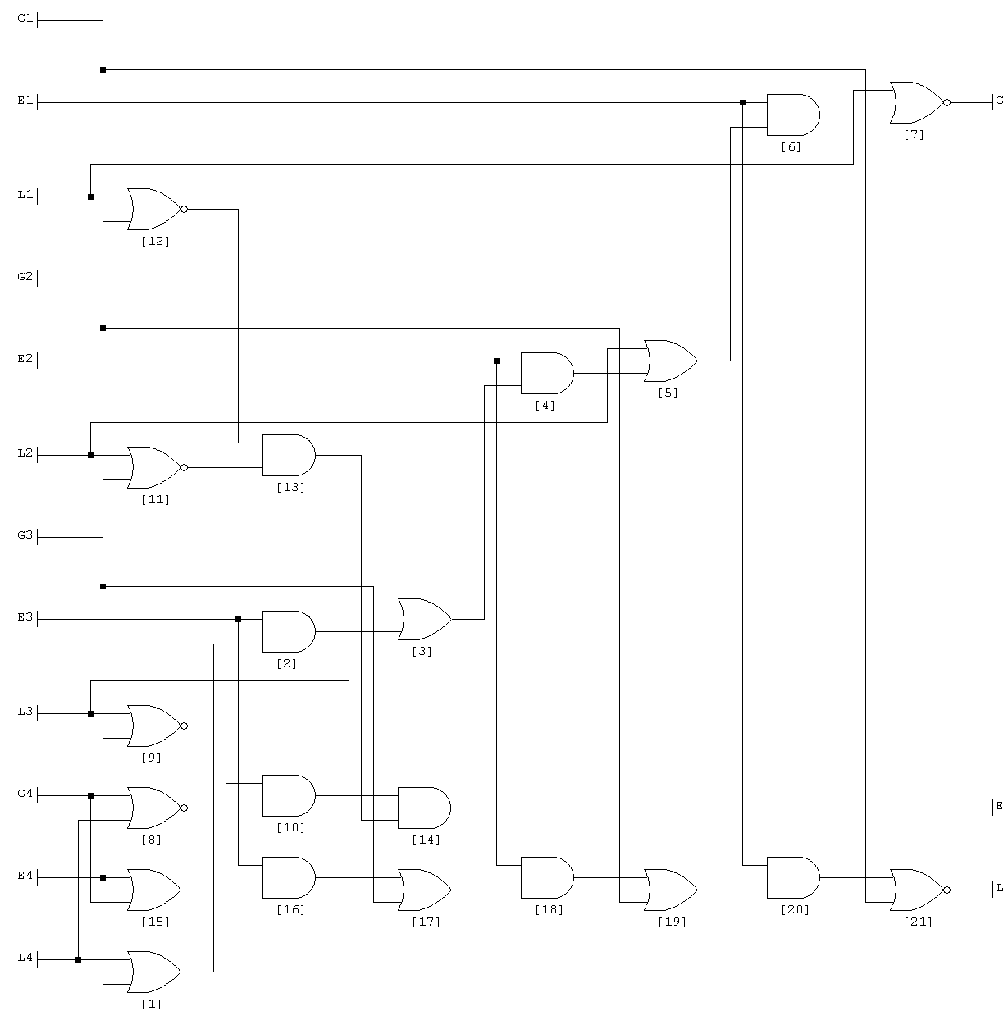
\includegraphics[max width = 0.95\textwidth]{Sol4-3} With L1, G1, E1 as the outputs from the highest four bits, and G4, E4, L4 as the output from the low bits.
                    % This is found via the truth table \lstinputlisting{./chapter04/FigHw/sol4-3.txt}
                    Connect four comparators in a daisy chain with the 16-bit inputs $X$ and $Y$ divided into four 4-bit sub-vectors sent to one of the 4-bit comparators.  The connect
                    the $G_{out}$, $L_{out}$, and $E_{out}$ signals of the more significant comparator to the $G_{in}$, $L_{in}$, and $E_{in}$ of the less significant comparator.
                    Hardwire the $G_{in}$, $L_{in}$, and $E_{in}$ inputs of the most significant comparator (the one with $X(15\ldots12)$ and $Y(15\ldots12)$ as the data inputs)
                    to $0,0,1$ respectively.  Use the  $G_{out}$, $L_{out}$, and $E_{out}$ of the leaqst significant comparator as the  $G_{out}$, $L_{out}$, and $E_{out}$ of the 
                    16-bit comparator.
                }
            \end{onlysolution}

        \item \textbf{ (2 pts.)}Determine the circuitry for the overflow detection
            circuit for a 2's-complement adder subtractor.  See page~\pageref{4-page:Ovf}.

            \begin{onlysolution} \textbf{Solutions} \itshape{
                    $
                    \begin{array} {c||c|c} \\
                        c_{in}  \bs c_{out} & 0 & 1 \\ \hline
                        0    &   & 1 \\ \hline
                        1    & 1 &   \\
                    \end{array}$   \\
                    Thus $ovf = c_{in}' c_{out} + c_{in} c_{out}' =  c_{in} \oplus c_{out} $
                }
            \end{onlysolution}

        \item \textbf{ (10 pts.)}Build a BCD to 7-Segment Display converter using
            Espresso.

            \begin{buildingblock}{BCD to 7-segment}
                \index{bcd to 7-segment}
                \label{page:7seg}
                \begin{tabular}{|l|p{3.5in}|} \hline
                    Nomenclature:  & BCD to 7-segment converter                \\ \hline
                    Data Input:    & 4-bit vector $D=d_3 d_2 d_1 d_0$  \\ \hline
                    Data Output:   & 7-bit vector $Y=y_6 \ldots y_1 y_0$    \\ \hline
                    Control:       & none                                   \\ \hline
                    Status:        & none                                   \\ \hline
                    Behavior:      & The output drives a 7-segment display pattern
                    representing the BCD digit.  \\ \hline
                \end{tabular}
            \end{buildingblock}

            A binary coded digit (BCD) is a 4-bit binary number that is constrained
            to assume the values of 0-9. That is, 1010 ... 1111 are illegal BCD digits.

            A 7-segment display is a box with seven inputs and seven output LED bars.
            Each input is wired to an LED bar that is illuminated when a 1 is applied
            to its input.
            Each of the seven LED segments is numbered according to the pattern shown
            on the left-hand side of Figure~\ref{fig:BCD}.

            \begin{figure}[ht]
                \center{\scalebox{0.7}{\includegraphics{Prob4-5}}}
                \caption{The numbering of the segments in a 7-segment display.
                The patterns of the BCD digits.}
                \label{fig:BCD}
            \end{figure}

            The pattern of LEDs to illuminate for each BCD digit is shown on the
            right-hand side of Figure~\ref{fig:BCD}.  A BCD to 7-segment converter
            has four inputs, $d_3 d_2 d_1 d_0$ and seven outputs $S_7 \ldots S_1$.
            Complete the design using Espresso.  Make sure to include ``Don't cares"
            in the truth table specification.
            \begin{enumerate}
                \item Use Espresso to determine the \SOPmin expression for the outputs
                    $S_7 \ldots S_1$.  Underline product terms that are shared.
                    Submit the Espresso source file.

                    \definecolorseries{BCD7-Table}{hsb}{step}[hsb]{0.35,0.42,1}{.368,0,-0.01} \resetcolorseries[10]{BCD7-Table}
                    \begin{onlysolution} \textbf{Solutions} \itshape{
                            The following is the source file for the BCD to 7-segment converter.\lstinputlisting{./chapter04/FigHw/sol4-5-a.txt}
                            This produces the following gates:\newpage
                            \begin{table}[t]
                                \centering
                                \begin{tabular}{llllll}
                                    s7 =&      \mathcolorbox{BCD7-Table!![0]}{(!d2\&!d1\&!d0)}        & +        \mathcolorbox{BCD7-Table!![2]}{(d1\&!d0)}                & +        \mathcolorbox{BCD7-Table!![6]}{(d2\&!d1\&d0)}         & +        \mathcolorbox{BCD7-Table!![9]}{(!d2\&d1)}                                                                               \\
                                    s6 =&      \mathcolorbox{BCD7-Table!![1]}{(d1\&d0)}               & +        \mathcolorbox{BCD7-Table!![3]}{(!d2\&!d1)}               & +        \mathcolorbox{BCD7-Table!![7]}{(d2\&!d1\&!d0)}        & +        \mathcolorbox{BCD7-Table!![5]}{(d2\&d1)}          & +        \mathcolorbox{BCD7-Table!![6]}{(d2\&!d1\&d0)}              \\
                                    s5 =&      \mathcolorbox{BCD7-Table!![0]}{(!d2\&!d1\&!d0)}        & +        \mathcolorbox{BCD7-Table!![2]}{(d1\&!d0)}                                                                                                                                                                                                                    \\
                                    s4 =&      \mathcolorbox{BCD7-Table!![2]}{(d1\&!d0)}              & +        \mathcolorbox{BCD7-Table!![4]}{(d2\&!d1\&!d0)}           & +        \mathcolorbox{BCD7-Table!![6]}{(d2\&!d1\&d0)}         & +        \mathcolorbox{BCD7-Table!![9]}{(!d2\&d1)}         & +        \mathcolorbox{BCD7-Table!![10]}{(d3)}                       \\
                                    s3 =&      \mathcolorbox{BCD7-Table!![1]}{(d1\&d0)}               & +        \mathcolorbox{BCD7-Table!![3]}{(!d2\&!d1)}               & +        \mathcolorbox{BCD7-Table!![7]}{(d2\&!d1\&!d0)}        & +        \mathcolorbox{BCD7-Table!![9]}{(!d2\&d1)}                                                                               \\
                                    s2 =&      \mathcolorbox{BCD7-Table!![0]}{(!d2\&!d1\&!d0)}        & +        \mathcolorbox{BCD7-Table!![4]}{(d2\&!d1\&!d0)}           & +        \mathcolorbox{BCD7-Table!![5]}{(d2\&d1)}              & +        \mathcolorbox{BCD7-Table!![6]}{(d2\&!d1\&d0)}     & +        \mathcolorbox{BCD7-Table!![10]}{(d3)}                       \\
                                    s1 =&      \mathcolorbox{BCD7-Table!![0]}{(!d2\&!d1\&!d0)}        & +        \mathcolorbox{BCD7-Table!![5]}{(d2\&d1)}                 & +        \mathcolorbox{BCD7-Table!![6]}{(d2\&!d1\&d0)}         & +        \mathcolorbox{BCD7-Table!![9]}{(!d2\&d1)}         & +        \mathcolorbox{BCD7-Table!![10]}{(d3)}               %
                                \end{tabular}
                            \end{table}

                        }
                    \end{onlysolution}

                \item Use Espresso to determine the \POSmin expression for the outputs
                    $S_7 \ldots S_1$.  Underline sum terms that are shared.
                    Submit the Espresso source file
                    \begin{onlysolution} \textbf{Solutions} \itshape {
                        If we run the same file as part a with the -epos flag, it will preform a minimization on the off-set of our functions. If we take this output and invert it, we will have our \POSmin expression.} \\
                        \begin{table}[h]
                            \centering
                            \begin{tabular}{*{7}{l}}
                                s7 =& \mathcolorbox{BCD7-Table!![0]}{(d3 + d2 + d1 + !d0)}  &$\&$ \mathcolorbox{BCD7-Table!![3]}{(!d2 + d1 + d0)}       &$\&$ \mathcolorbox{BCD7-Table!![5]}{(!d3 + !d0)}       &$\&$ \mathcolorbox{BCD7-Table!![4]}{(!d2 + !d1 + !d0)} & ~ & ~ \\
                                s6 =& \mathcolorbox{BCD7-Table!![1]}{(d2 + !d1 + d0)}       & ~                     & ~ & ~ & ~ & ~ \\
                                s5 =& \mathcolorbox{BCD7-Table!![2]}{(!d2 + d1 + !d0)}      &$\&$ \mathcolorbox{BCD7-Table!![0]}{(d3 + d2 + d1 + !d0)}  &$\&$ \mathcolorbox{BCD7-Table!![6]}{(d2 + !d1 + !d0)}  &$\&$ \mathcolorbox{BCD7-Table!![3]}{(!d2 + d1 + d0)}   &$\&$ \mathcolorbox{BCD7-Table!![5]}{(!d3 + !d0)} &$\&$ \mathcolorbox{BCD7-Table!![4]}{(!d2 + !d1 + !d0)} \\
                                s4 =& (d3 + d2 + d1)        &$\&$ \mathcolorbox{BCD7-Table!![4]}{(!d2 + !d1 + !d0)}     & ~ & ~ & ~ & ~ \\
                                s3 =& (!d2 + !d1 + d0)      &$\&$ \mathcolorbox{BCD7-Table!![2]}{(!d2 + d1 + !d0)}      & ~ & ~ & ~ & ~ \\
                                s2 =& \mathcolorbox{BCD7-Table!![1]}{(d2 + !d1 + d0)}       &$\&$ \mathcolorbox{BCD7-Table!![0]}{(d3 + d2 + d1 + !d0)}  &$\&$ \mathcolorbox{BCD7-Table!![6]}{(d2 + !d1 + !d0)}  & ~ & ~ & ~ \\
                                s1 =& \mathcolorbox{BCD7-Table!![0]}{(d3 + d2 + d1 + !d0)}  &$\&$ \mathcolorbox{BCD7-Table!![3]}{(!d2 + d1 + d0)}       & ~ & ~ & ~ & ~ \\
                            \end{tabular}
                        \end{table}
%% \begin{verbatim}
%% # BCD to 7-segment display
%% #
%% .i 4
%% .o 7
%% .ilb b3 b2 b1 b0
%% .ob s7 s6 s5 s4 s3 s2 s1
%% #.phase 0000000
%% .p 9
%% 000- 0001000
%% -110 0000100
%% -010 0100010
%% -101 0010100
%% 0001 1010011
%% -011 0010010
%% -100 1010001
%% 1--1 1010000
%% -111 1011000
%% .e
%% \end{verbatim}
                    \end{onlysolution}
            \end{enumerate}

            \filbreak % Strongly suggest page break
        \item \textbf{(10 pts.)} Build a box which has one 4-bit input called A and
            one 4-bit output called T. The output T is the 2's-complement value
            of the input A.  Use the bit slice paradigm to solve this
            problem.  That is, create a building block for one bit of the problem
            then string four of them together to solve the problem.
            For the problem at hand this can be done as follows:
            \begin{enumerate}
                \item Start at the LSB of A.
                \item If this is the first, least significant, 1, flip all bits
                    to the left.
                \item If this is not the first 1, leave the bit alone.
                \item Move one bit to the left.
                \item Goto Step b.
            \end{enumerate}
            A bit-slice should communicate whether there has been a 1 to the right,
            to the more significant bit.  Submit:
            \begin{itemize}
                \item How the above "algorithm" behaves when presented with
                    the inputs A=1100
                    \begin{onlysolution}
                        \textit{\color{blue}
                            \begin{enumerate}
                                \item Move one bit to the left
                                \item Move one bit to the left
                                \item Flip. Move one bit to the left
                                \item Flip. Move one bit to the left
                            \end{enumerate}}
                    \end{onlysolution}
                \item The truth table for one bit slice
                    \begin{onlysolution}

                    \end{onlysolution}
                \item \SOPmin expression and circuit diagram for a bit slice.
                    \begin{onlysolution}

                    \end{onlysolution}
                \item The organization of four bit slices to solve the problem
                    \begin{onlysolution}

                    \end{onlysolution}
            \end{itemize}

            \begin{onlysolution} \textbf{Solutions} \itshape{
                    The key to the begin solution  is to figure out the structure
                    of the begin solution  and then give meaning to the signals involved.
                    The problem will be sliced into four bit-slices; each handled
                    but its own complement box.  Thus, there will be four complement
                    box in the begin solution.  Each box will have 2 inputs, one being
                    a bit of A and the other being a "carry in" from the less
                    significant less, immediately to the right.  Each box
                    will have two bits of output, a bit of T and a "carry out".
                    The carry bits (both into and out of a box will convey
                    information regarding the rightmost 1 in the number A.)

                    If the carry in is equal 1 then there is a one to the right.
                    If the carry in is equal 0 then there is not a one to the right.
                    The truth table for a box is then

                    \begin{table}[h]
                        \begin{tabular}{l|l||l|l|l}
                            $A$ & $c_{in}$  & $T$ & $c_{out}$ & comment \\ \hline
                            0   & 0       &   0 & 0          & There is no 1 to the right \\ \hline
                            0   & 1       &   1 & 1          & There is a 1 to the right, flip A \\ \hline
                            1   & 0       &   1 & 1          & There is is no 1 to the right, but we've
                            created one \\ \hline
                            1   & 1       &   0 & 1          & There is a 1 to the right, flip A \\
                        \end{tabular}
                    \end{table}

                    From this it follows that: \\
                    $T=A'c_{in} + A c_{in}'=A \oplus c_{in}$ \\
                    $c_{out} = A + c_{in}$
                }
            \end{onlysolution}
        \item \textbf{(4 pts.)} Build a 7:128 decoder using a minimum number of
            4:16, 2:4 and 1:2 decoders. Describe the wiring of the select lines.

            \begin{onlysolution} \textbf{Solutions}
                \begin{figure}[h]
                    \centering
                    \includegraphics[height=0.8\textheight]{Sol4-7}
                    \caption{A 7:128 decoder built from 4:16, 2:4 and 1:2 decoders.}
                    \label{fig:bighwdec}
                \end{figure}
                \filbreak
            \end{onlysolution}
        \item \textbf{(4 pts. each)} Design a circuit with two 8-bit inputs $X,Y$, an
            8-bit output $Z$ and a 1-bit input $sel$.  Construct a circuit that yields the
            correct value of $Z$ using only the basic building blocks presented in this
            chapter; do NOT show the internal organization of these building blocks.  If
            a mux is used, denote which input is the $y_0$ and which is $y_1$.
            If a comparator is used denote which input is $X$ and which is $Y$.
            Do not use any AND or OR gates; it will tempting in the later problems.
            \begin{enumerate}
                \item \verb^ if (sel==0) then Z = X else Z = Y ^

                    \begin{onlysolution} \textbf{Solutions} \itshape{
                            \includegraphics{Sol4-8a}
                        }
                    \end{onlysolution}

                \item \verb^ if (sel==0) then Z = X+Y else Z = Y ^

                    \begin{onlysolution} \textbf{Solutions} \itshape{
                            \includegraphics{Sol4-8b}
                        }
                    \end{onlysolution}

                \item \verb^ if (sel==0) then Z = X+Y else Z = X-Y ^

                    \begin{onlysolution} \textbf{Solutions} \itshape{
                            \includegraphics{Sol4-8c}
                        }
                    \end{onlysolution}

                \item \verb^ if (X==0) then Z = X else Z = Y ^

                    \begin{onlysolution} \textbf{Solutions} \itshape{
                            \includegraphics{Sol4-8d}
                        }
                    \end{onlysolution}

                \item \verb^ if (X==Y) then Z = X-Y else Z = Y ^

                    \begin{onlysolution} \textbf{Solutions} \itshape{
                            \includegraphics{Sol4-8e}
                        }
                    \end{onlysolution}

                \item \verb^ if (X==Y) then Z = X+Y else Z = X-Y ^

                    \begin{onlysolution} \textbf{Solutions} \itshape{
                            \includegraphics{Sol4-8f}
                        }
                    \end{onlysolution}

                \item \verb^ if (X < Y) then Z = X else Z = Y ^

                    \begin{onlysolution} \textbf{Solutions} \itshape{
                            \includegraphics{Sol4-8g}
                        }
                    \end{onlysolution}

                \item \verb^ if (X <= Y) then Z = X else Z = Y ^

                    \begin{onlysolution} \textbf{Solutions} \itshape{
                            \includegraphics{Sol4-8h}
                        }
                    \end{onlysolution}

                \item \verb^ if (X > Y) then Z = X else Z = Y ^

                    \begin{onlysolution} \textbf{Solutions} \itshape{
                            \includegraphics{Sol4-8i}
                        }
                    \end{onlysolution}

                \item \verb^ if (X > Y) then Z = X+X else Z = Y+Y ^

                    \begin{onlysolution} \textbf{Solutions} \itshape{
                            \includegraphics{Sol4-8j}
                        }
                    \end{onlysolution}

            \end{enumerate}

        \item \textbf{ (10 pts.)} Build a 4-bit priority encoder.

            \begin{buildingblock}{Priority Encoder}
                \index{priority encoder}
                \begin{tabular}{|l|p{3.5in}|} \hline
                    Nomenclature:  & N-bit priority encoder                \\ \hline
                    Data Input:    & N-bit vectored  $D=d_{N-1} \ldots d_1 d_0$  \\ \hline
                    Data Output:   & $\log_2(N)$-bit vector $Y=y_{log_2(N)} \ldots y_1 y_0$    \\ \hline
                    Control:       & none                    \\ \hline
                    Status:        & none                                   \\ \hline
                    Behavior:      & $F = i$ where $i$ is the highest indexed input
                    which equals 1.  When all inputs equal
                    0, the output is a ``don't care".  \\ \hline
                \end{tabular}
                \label{page:prior}
            \end{buildingblock}

            The idea is for the outputs to represent (in binary code) the highest
            input index which equals 1.  For example, a 4-bit priority encoder
            with input $D=1010$ has inputs $d_3=1$ and $d_0=1$.  Of these two
            inputs, the index of $d_3$ is greater than the index of $d_0$ so the
            output, $F$ is equal to 3, or in binary $11$.  If the input were
            $D=0111$ then $F=10$.

            \begin{enumerate}
                \item Write down the truth table for a 4-bit priority encoder.  Hint,
                    the truth table could be structured so that it contains only five rows
                    by using ``don't cares" on the inputs.

                    \begin{onlysolution} \textbf{Solutions} \itshape{
                            \begin{tabular}{l|l|l|l||l|l}
                                $d_3$ & $d_2$ & $d_1$ & $d_0$ & $f_1$ & $F_0$ \\ \hline
                                0  &    0  &    0  &    0  &    x  &    x  \\ \hline
                                0  &    0  &    0  &    1  &    0  &    0  \\ \hline
                                0  &    0  &    1  &    x  &    0  &    1  \\ \hline
                                0  &    1  &    x  &    x  &    1  &    0  \\ \hline
                                1  &    x  &    x  &    x  &    1  &    1  \\
                            \end{tabular}
                        }
                    \end{onlysolution}

                \item An \SOPmin realization of the circuit.
                    \begin{onlysolution} \textbf{Solutions} \itshape{
                            $f_1 = d_3 + d_2$ \\
                            $f_0 = d_3 + d_2'd_1$
                        }
                    \end{onlysolution}
            \end{enumerate}

        \item \textbf{ (10 pts.)} Build a 4-bit saturation adder.  A
            saturation adder performs normal 4-bit addition when the
            resulting sum is less than 15.  If the sum is
            greater than 15, the saturation adders outputs 15.  The
            following table summarizes.

            \begin{buildingblock}{Saturation Adder}
                \index{saturation adder}
                \label{page:saturation}
                \begin{tabular}{|l|p{3.5in}|} \hline
                    Nomenclature:  & 4-bit saturation adder                \\ \hline
                    Data Input:    & 2, 4-bit vectors \verb+A, B+  \\ \hline
                    Data Output:   & 4-bit vector \verb+sum+    \\ \hline
                    Control:       & none                                   \\ \hline
                    Status:        & none                                   \\ \hline
                    Behavior:      &
                \begin{verbatim}
                if (A+B > 15) sum = 15
                else sum = A+B
                \end{verbatim}
                    \\ \hline
                \end{tabular}
            \end{buildingblock}

            Submit a schematic showing the basic building blocks, their
            data status, and control interconnections.  Show any truth
            tables used to build glue logic.

            \begin{onlysolution} \textbf{Solutions} \itshape{
                    All we need to do is to determine when the sum is greater then
                    15 and output 15 when it is.  The comparator/mux combo mentioned
                    several times in the chapter should do the trick.

                    \includegraphics{Sol4-10}

                }
            \end{onlysolution}

        \item \textbf{ (10 pts.)} Build a mod-6 adder.  The mod-6 adder
            takes as input two 3-bit (mod 6) numbers and adds them together
            modulus 6.

            \index{modular arithmetic}
            \label{page:mod}
            Modular arithmetic only operates with a limited portion of the
            integers.  The range of numbers is $\{0,1,2, \ldots ,m-1\}$ where
            $m$ is called the \textit{ modulus}; note there are $m$ different
            integers because counting started at 0.  For example, when working
            in mod-6 arithmetic use the integers $\{0,1,2,3,4,5\}$.
            To solve any addition problem in modular arithmetic, it is only
            necessary to perform regular addition with the special rule that
            the addition process rolls over from the largest number, $m-1$ to 0
            when the result is larger than $m-1$.  For
            example, in mod-6 arithmetic $(5+1) \mod 6 = 0$.  The statement
            ``$\mod 6$" is always included in the addition problem to indicate
            to the reader that mod-6 arithmetic is being performed.  Here
            are a few more examples to help

            \begin{tabular}{l}
                $2+3~\mod 6 = 5$ \\
                $3+3~\mod 6 = 0$ \\
                $4+3~\mod 6 = 1$ \\
                $5+5~\mod 6 = 4$
            \end{tabular}

            \index{modular adder}
            \label{page:modadder}
            \begin{tabular}{|l|p{3.5in}|} \hline
                Nomenclature:  & 3-bit mod 6 adder                \\ \hline
                Data Input:    & two, 3-bit (mod-6) vectors \verb+A, B+  \\ \hline
                Data Output:   & 3-bit (mod-6) vector \verb+sum+    \\ \hline
                Control:       & none                                   \\ \hline
                Status:        & none                                   \\ \hline
                Behavior:      &
                \begin{verbatim}
                sum = A+B mod 6
                \end{verbatim}
                \\ \hline
            \end{tabular}

            Submit a schematic showing the basic building blocks, their
            data status, and control interconnections.  Show any truth
            tables used to build glue logic.  Be careful that the word
            size of the result is handled correctly.

            \begin{onlysolution} \textbf{Solutions} \itshape{
                    Since the inputs are mod 6 numbers then the inputs can be in the
                    range [0-5].  Adding two such values will yield a value in the
                    range [0-10].  Hence a simple adjustment of the sum when its larger
                    that 5 is required.

                    \includegraphics{Sol4-11}

                }
            \end{onlysolution}

        \item \textbf{ (1pt. each)}Convert the following to 2's-complement
            assuming a word size of eight bits.
            \begin{enumerate}
                \item -35

                    \begin{onlysolution} \textbf{Solutions} \itshape{
                            $35 = 32+2+1 = 100011 = 00100011$, thus $-35=11011101$
                        }
                    \end{onlysolution}

                \item  -128

                    \begin{onlysolution} \textbf{Solutions} \itshape{
                            This is a special case, see page 10 for more information.
                            $-128 = 10000000$
                        }
                    \end{onlysolution}

                \item  67

                    \begin{onlysolution} \textbf{Solutions} \itshape{
                            $67=64+2+1 = 100 0011 = 0100 0011$
                        }
                    \end{onlysolution}

                \item  128

                    \begin{onlysolution} \textbf{Solutions} \itshape{
                            There are not enough bits to represent this positive number; hence
                            the 8-bit representation does not exist.
                        }
                    \end{onlysolution}

            \end{enumerate}
            \filbreak
        \item \textbf{ (1 pt. each)} Perform the following operations for the given
            2's-complement numbers. Assume a word size of eight bits
            in all cases. Indicate where overflow occurs. If there is no overflow,
            convert the result to decimal.
            \begin{enumerate}

                \item 01011101 + 00110111

                    \begin{onlysolution} \textbf{Solutions}
                        \begin{align*}
                            {\color{gray}
                            1111\,111\0 }&\\[-1.5ex]
                            0101\,1101&\\
                            +\:0011\,0111&\\[-2ex]
                            \rule{12ex}{1pt}\hspace{-1ex}&\\[-1ex]
                            1001\,0100&\quad  overflow
                        \end{align*}
                    \end{onlysolution}

                \item 11101011 + 11110001

                    \begin{onlysolution} \textbf{Solutions}
                        \begin{align*}
                            {\color{gray}
                            111\0\0\911\0 }&\\[-1.5ex]
                            1110\,1011&\\
                            +\:1111\,0001&\\[-2ex]
                            \rule{12ex}{1pt}\hspace{-1ex}&\\[-1ex]
                            1101\,1100&
                        \end{align*}
                    \end{onlysolution}

                \item 01011101 + 10101011

                    \begin{onlysolution} \textbf{Solutions}
                        \begin{align*}
                            {\color{gray}
                            11111\,111\0}&\\[-1.5ex]
                            0101\,1101&\\
                            +\:1010\,1011&\\[-2ex]
                            \rule{12ex}{1pt}\hspace{-1ex}&\\[-1ex]
                            0000\,1000&
                        \end{align*}
                    \end{onlysolution}

                \item 10111011 - 11110001

                    \begin{onlysolution} \textbf{Solutions}
                        \begin{alignat*}{3}
                            &&{\color{gray}
                            1\,111\0 }\\[-1.5ex]
                            1110\,1011&   &1110\,1011\\
                            -\:1111\,0001&&+\:0000\,1111\\[-2ex]
                            \rule{12ex}{1pt}\hspace{-1ex}&\ \raisebox{3.5ex}[0pt][0pt]{$\xLongrightarrow{\phantom{80em}}$}\ &\rule{12ex}{1pt}\hspace{-1ex}\\[-1ex]
                            & &1101\,1010
                        \end{alignat*}
                    \end{onlysolution}

                \item 01011101 - 00110111

                    \begin{onlysolution} \textbf{Solutions}
                        \begin{alignat*}{3}
                            &&{\color{gray}
                            11\011\9\01\0 }\\[-1.5ex]
                            0101\,1101&&   0101\,1101\\
                            -\:0011\,0111&&+\:1100\,1001\\[-2ex]
                            \rule{12ex}{1pt}\hspace{-1ex}&\ \raisebox{3.5ex}[0pt][0pt]{$\xLongrightarrow{\phantom{80em}}$}\ &\rule{12ex}{1pt}\hspace{-1ex}\\[-1ex]
                            &&   0010\,0110
                        \end{alignat*}
                    \end{onlysolution}

                \item 01011101 - 10101111

                    \begin{onlysolution} \textbf{Solutions}
                        \begin{alignat*}{3}
                            &&{\color{gray}
                            \1 1\9\0\01\0 }\\[-1.5ex]
                            0101\,1101&&   0101\,1101\\
                            -\:1010\,1111&&+\:0101\,0001\\[-2ex]
                            \rule{12ex}{1pt}\hspace{-1ex}&\ \raisebox{3.5ex}[0pt][0pt]{$\xLongrightarrow{\phantom{80em}}$}\ &\rule{12ex}{1pt}\hspace{-1ex}\\[-1ex]
                            &&1010\,1110&\ \textit{overflow}
                        \end{alignat*}
                    \end{onlysolution}

            \end{enumerate}

        \item \textbf{ (10 pts.)}
            \label{page:flipbox}
            Build a flip box.  A flip box is defined by the following input,
            output, and behavior definition.

            \begin{tabular}{|l|p{3.5in}|} \hline
                Nomenclature:  & 8-bit flip box.                    \\ \hline
                Data Input:    & 8-bit $D=d_7 \ldots d_0$          \\ \hline
                Data Output:   & 8-bit $F=f_7 \ldots f_0$          \\ \hline
                Control:       & 3-bit $S=s_2 s_1 s_0$            \\ \hline
                Status:        & none                                   \\ \hline
                Behavior:      & The output is the same as the input except for
                one bit which is inverted.  The index of the inverted
                bit is given by $S$. \\ \hline
            \end{tabular}

            The flip box takes the 8-bit data input, flips a single bit identified
            by $S$, then sends the new 8-bit value to the output.
            For example, if $D=11110000$ and $S=010$ then
            $F=11110100$.  If $D=11110000$ and $S=101$ then $F=11010000$.  The solution
            should rely heavily on the basic building blocks.

            \begin{onlysolution} \textbf{Solutions} \itshape{
                    Arrange 8, 2:1 muxes with $d_i$ and $d_i'$ going into the data inputs.
                    Run the select into a 3:8 decoder and route the data outputs to the
                    individual selects of the 2:1 muxes.
                }
            \end{onlysolution}

        \item \textbf{(10 pts.)}
            \label{page:IsScan}
            Build a box which recognizes some keyboard scancode.  When a key is
            pressed on a keyboard, the keyboard transmits (among other things)
            an 8-bit scancode of the pressed key.  Each key has its own scancode
            listed in Table~\ref{table:scancodes}.  The relationship between the
            keys and their scancode is not based on ASCII.

            \begin{table}[h]
                \begin{tabular}{|l|l||l|l||l|l||l|l|} \hline
                    Key & scancode & Key & scancode & Key & scancode & Key & scancode \\ \hline \hline
                    0 & $45_{16}$ & 1 & $16_{16}$ & 2 & $1E_{16}$ & 3 & $26_{16}$ \\ \hline
                    4 & $25_{16}$ & 5 & $2E_{16}$ & 6 & $36_{16}$ & 7 & $3D_{16}$ \\ \hline
                    8 & $3E_{16}$ & 9 & $46_{16}$ & A & $1C_{16}$ & B & $32_{16}$ \\ \hline
                    C & $21_{16}$ & D & $23_{16}$ & E & $24_{16}$ & F & $2B_{16}$ \\ \hline
                    P & $4D_{16}$ & L & $4B_{16}$ & M & $3A_{16}$ & I & $43_{16}$ \\ \hline
                \end{tabular}
                \caption{IBM 6450225 Keyboard scancodes.}%\footnote{it is based on an \href{https://www.seasip.info/VintagePC/ibm_6450225.html}{IBM 6450225 Keyboard}}
                \label{table:scancodes}
            \end{table}
            \label{page:scanclass}
            \begin{tabular}{|l|p{3.5in}|} \hline
                Nomenclature:  & scancode classifier                   \\ \hline
                Data Input:    & 8-bit $D=d_7 \ldots d_0$          \\ \hline
                Data Output:   & IsP, IsL, IsM, IsI, IsS \\ \hline
                Control:       & none             \\ \hline
                Status:        & none                                   \\ \hline
                Behavior:      & IsP =1 when $D$ is the scan code for the letter ``P".
                IsL =1 when $D$ is the scan code for the letter ``L".
                IsM =1 when $D$ is the scan code for the letter ``M".
                IsI =1 when $D$ is the scan code for the letter ``I".\\ \hline
                %IsS =1 when $D$ is the scan code for the letter ``S".{\color{blue}($1B_{16}$)}  \\ \hline
            \end{tabular}\\
            \begin{onlysolution} \textbf{Solution:}
                \textit{\color{blue} We would simply need 4 comparators testing if the incoming scan code is equal to $4D_{16}$ (IsP), $4B_{16}$ (IsL), $3A_{16}$ (IsM), or $43_{16}$ (IsI).}\\
                \includegraphics[max width = 0.8\textwidth]{sol4-15}

            \end{onlysolution}
            \filbreak
        \item \textbf{(10 pts.)}
            \label{page:ScanDecode}
            Build a box which converts an 8-bit scancode for a hexadecimal digit into a 4-bit hexadecimal values.

            \label{page:scanconv}
            \begin{tabular}{|l|p{3.5in}|} \hline
                Nomenclature:  & scancode classifier                   \\ \hline
                Data Input:    & 8-bit $D=d_7 \ldots d_0$          \\ \hline
                Data Output:   & 4-bit $H=h_3h_2h_1h_0$ \\ \hline
                Control:       & none             \\ \hline
                Status:        & none                                   \\ \hline
                Behavior:      & Converts the scancode $D$, representing a the
                key of a hexadecimal character, into its 4-bit
                value $H$.
                \\ \hline
            \end{tabular}

            For example, if $D=25_{16}$, the scancode for the "4" key, then the converter
            should output $H=0100_2$.  Assume that the inputs are always
            legal hexadecimal scancodes.
            \begin{onlysolution}
                {\color{blue}

                    \begin{table}[!ht]
                        \centering
                        {\color{blue}
                            \lstinputlisting{./chapter04/FigHw/sol4-16.txt   }
                            \lstinputlisting{./chapter04/FigHw/sol4-16-ex.txt}
                        }
                \end{table}}
            \end{onlysolution}
    \end{enumerate}


\include{./chapter05/chapter5}
\section{Exercises}
\label{section:sequentialCircuitsExercises}
\graphicspath{ {./chapter05/FigHw} }

\begin{enumerate}

    \item \textbf{ (8 pts.)}Determine the state table for the circuit in Figure~\ref{fig:sequentialCirNANDs}.
        \begin{figure}[ht]
            \center{\includegraphics{Prob5-1}}
            \caption{}
            \label{fig:sequentialCirNANDs}
        \end{figure}

        \begin{onlysolution}  \textbf{Solution} \itshape{
                The analysis of the cross-coupled NANDs show in Figure~\ref{fig:sequentialCirNANDs} is
                almost exactly the same as that for the cross coupled NORs.  Start with
                the truth table for an NAND gate:

                \begin{tabular}{l|l||l}
                    a & b & (ab)' \\ \hline
                    0 & 0 & 1 \\ \hline
                    0 & 1 & 1 \\ \hline
                    1 & 0 & 1 \\ \hline
                    1 & 1 & 0 \\
                \end{tabular}

                Observe that the output is 1 whenever
                either input is 0.  Now onto the state table for the cross coupled NANDs:

                \begin{tabular}{l|l||l|l}
                    A & B & $F^+$ & $G^+$ \\ \hline
                    0 & 0 & 1 & 1 \\ \hline
                    0 & 1 & 1 & 0 \\ \hline
                    1 & 0 & 0 & 1 \\ \hline
                    1 & 1 & F & G \\
                \end{tabular}

                For the cross coupled NANDs the output holds when the input $A,B=1,1$ occurs.
                In fact if you compare this table to that of the cross coupled NORs, you will
                notice that $A,B = S',R'$ and $F,G = Q,Q'$.
            }
        \end{onlysolution}

    \item \textbf{ (8 pts.)} Determine the state table for the circuit
        in Figure~\ref{fig:sequentialCirDLatch}.  Which basic memory element does it act
        like?  Hint, one of the inputs is acting like a clock.  Additional
        hint, in order to simplify the analysis, replace a portion of the
        circuit with a component from this chapter.
        \begin{figure}[ht]
            \center{\includegraphics{Prob5-2}}
            \caption{}
            \label{fig:sequentialCirDLatch}
        \end{figure}

        \begin{onlysolution}  \textbf{Solution} \itshape{
                The main idea in this problem is to simplify the cross coupled NOR gates into
                an SR latch.  Then use the state table for the SR latch.  This substitution
                will simplify the analysis of this circuit.  Since the lower NOR gate is denoted
                $A$, call the lower input of the SR latch $R$ and the upper input $S$
                (see Figure 5.6).

                This yields the following truth table:

                \begin{tabular}{l|l|l|l|l||l}
                    A & B & S & R & comment & $Q^+$ \\ \hline
                    0 & 0 & 0 & 0 & Hold    & $Q$   \\ \hline
                    0 & 1 & 0 & 0 & Hold    & $Q$   \\ \hline
                    1 & 0 & 0 & 1 & Reset   & 0     \\ \hline
                    1 & 1 & 1 & 0 & Set     & 1     \\
                \end{tabular}

                It is behaving exactly like a D clocked latch, where $A=clk$ and $B=D$.
            }
        \end{onlysolution}

    \item \textbf{ (8 pts.)} Complete the timing diagram for the circuit
        shown in Figure~\ref{fig:sequentialCirDMS}.  Which basic memory element
        does this circuit act like?

        \ifshowanswers \textbf{Solution} \fi

        \begin{figure}[ht]
            \label{fig:sequentialCirnand}
            \center{\scalebox{0.8}{
                    \ifshowanswers \includegraphics{sol5-3}
                    \else \includegraphics{prob5-3}\fi
            }}
            \caption{A 2-stage sequential circuit.}
            \label{fig:sequentialCirDMS}
        \end{figure}
        \ifshowanswers \textit{\color{blue} This circuit is acting like a Negative Edge Triggered D Flip Flop.}\fi
        \filbreak %h! won't prevent content beneath it from filling, so we need to give it some help with keeping them together
    \item \textbf{ (15 pts.)} Complete the timing diagram for the basic memory
        elements in Figure~\ref{fig:sequentialCirExTim}.  The clock cycle is 20 ns. When
        necessary, assume that $Q$ is initialized to 0 and the output settles to
        0 after a period of rapid toggling. \needspace{4.78in} % tell it that we really do want it to keep this question next to the figure
        \ifshowanswers \textbf{Solution} \fi
        \begin{figure}[ht]
            \center{\scalebox{0.5}{
                    \ifshowanswers \includegraphics{sol5-4} \else \includegraphics{prob5-4} \fi
            }}
            \caption{A variety of basic memory elements and the signals applied to them.}
            \label{fig:sequentialCirExTim}
        \end{figure}
    \item \textbf{ (15 pts.)} Complete the timing diagram for the basic memory elements in
        Figure~\ref{fig:sequentialCirExTim2}.  The clock cycle is 20 ns. When necessary,
        assume that Q is initialized to 0 and the output settles to 0 after
        a period of rapid toggling.\par
        \ifshowanswers \textbf{Solution} \fi
        \begin{figure}[ht]
            \center{\scalebox{0.5}{
                    \ifshowanswers \includegraphics{sol5-5} \else \includegraphics{prob5-5} \fi
            }}
            \caption{}
            \label{fig:sequentialCirExTim2}
        \end{figure}
        \filbreak
    \item \textbf{ (4 pts.)} Consider the furnace
        controller discussed at the beginning of this chapter.  Determine
        which state the controller should transition into when in a particular state
        and given a particular combination of inputs.
        Fill in the eight entries in the following table with the next state
        the system should move into.  The next state should be either ON if the
        system should transition (or remain in) the ON state, OFF if the system
        should transition (or remain in) the OFF state, or X if the input
        combination is meaningless.
        \begin{onlyproblem} % Compress the problem version as it can be trivially recreated
            \center{
                \begin{tabular}{c||c|c|c|c}CurrentState$\bs~T_{hi}T_{low}$&00&01&11&10\\\hline\hline ON&&&&\\ \hline OFF&&&&\\
            \end{tabular}}
        \end{onlyproblem}
        \begin{onlysolution}
            \center{
                \begin{tabular}{c||c|c|c|c}
                    Current State $\bs T_{hi} T_{low}$ & 00  & 01 & 11 & 10  \\ \hline \hline
                    ON                                 & ON  & ON & X  & OFF \\ \hline
                    OFF                                & OFF & ON & X  & OFF \\
            \end{tabular}}
        \end{onlysolution}

    \item \textbf{ (8 pts.)} Derive the next state equations for each
        type (D, T, SR, and JK) of basic memory element.  The next state equation
        is a symbolic equation describing the next state ($Q^+$)
        as a function of the inputs (D,T,SR, or JK) and state ($Q$).
        In order to determine the next state equations for a
        a JK memory element, build a 3-variable Kmap with
        $Q$, $J$, and $K$ as the inputs.  The entries in the Kmap should
        be $Q^+$.  Solving this Kmap will yield the next state equation.
        Show all work for full credit.
        \begin{onlysolution}
            \begin{figure}[ht]
                \center{\includegraphics{sol5-7-DC}}
                \caption{}
            \end{figure}
            {\color{blue}\addtolength{\tabcolsep}{-0.4em}
                \begin{tabular}{*{3}{l}}
                    $Q^+_D   $   &$= D         $& ~                              \\[0.1em]
                    $Q^+_T   $   &$= Q'T + QT' $&$= (Q+T)(Q'+T') = Q\oplus T$    \\[0.1em]
                    $Q^+_{SR}$   &$= SR'+R'Q   $&$= (Q+S)(R')   $                \\[0.1em]
                    $Q^+_{JK}$   &$= Q'J + QK' $&$= (Q+J)(Q'+K')$
            \end{tabular}}
        \end{onlysolution}
    \item \textbf{ (16 pts.)} Derive the transition list for each
        type (D, T, SR, and JK) of basic memory element.  A transition
        list describes the input(s) necessary to elicit a particular
        change in state.  For example, imagine that a D flip flop output
        is currently in the 0 state and it needs to transition to
        the 1 state after the clock edge.  In other words, $Q=0$ and
        $Q^+ = 1$.  What input would have to be provided on the
        $D$ input to make this happen?  Clearly, $D=1$.  This entry
        is filled in Table~\ref{table:tl}.

        Hint, the Kmaps used to determine the next state equations
        will help in visualizing all the conditions which elicit
        a particular change of input.  Complete the transition list
        for all four memory types.  For full credit, show how the
        entries in the transition list are determined.

        \begin{table}[ht]
            \center{
                \begin{onlyproblem}
                    \begin{tabular}{cccc}
                        \begin{tabular}{c||c}$Q\rightarrow~Q^+$&D\\\hline\hline$0\rightarrow0$&\\\hline$0\rightarrow1$&1\\\hline$1\rightarrow0$&\\\hline$1\rightarrow1$&\\
                        \end{tabular}&
                        \begin{tabular}{c||c}$Q\rightarrow~Q^+$&T\\\hline\hline$0\rightarrow0$&\\\hline$0\rightarrow1$&\\\hline$1\rightarrow0$&\\\hline$1\rightarrow1$&\\
                        \end{tabular}&
                        \begin{tabular}{c||c|c}$Q\rightarrow~Q^+$&S&R\\\hline\hline$0\rightarrow0$&&\\\hline$0\rightarrow1$&&\\\hline$1\rightarrow0$&&\\\hline$1\rightarrow1$&&\\
                        \end{tabular}&
                        \begin{tabular}{c||c|c}$Q\rightarrow~Q^+$&J&K\\\hline\hline$0\rightarrow0$&&\\\hline$0\rightarrow1$&&\\\hline$1\rightarrow0$&&\\\hline$1\rightarrow1$&&\\
                        \end{tabular}\\
                    \end{tabular}
                \end{onlyproblem}
                \begin{onlysolution}{\color{blue}
                        \begin{tabular}{cccc}

                            \begin{tabular}{c||c}
                                $Q \rightarrow Q^+$ &   D           \\ \hline \hline
                                $0 \rightarrow 0$   &   0           \\ \hline
                                $0 \rightarrow 1$   &   1           \\ \hline
                                $1 \rightarrow 0$   &   0           \\ \hline
                                $1 \rightarrow 1$   &   1           \\
                            \end{tabular}

                            &

                            \begin{tabular}{c||c}
                                $Q \rightarrow Q^+$ &   T           \\ \hline \hline
                                $0 \rightarrow 0$   &   0           \\ \hline
                                $0 \rightarrow 1$   &   1           \\ \hline
                                $1 \rightarrow 0$   &   1           \\ \hline
                                $1 \rightarrow 1$   &   0           \\
                            \end{tabular}

                            &

                            \begin{tabular}{c||c|c}
                                $Q \rightarrow Q^+$ &   S   &   R   \\ \hline \hline
                                $0 \rightarrow 0$   &   0   &   0,1 \\ \hline
                                $0 \rightarrow 1$   &   1   &   0   \\ \hline
                                $1 \rightarrow 0$   &   0   &   1   \\ \hline
                                $1 \rightarrow 1$   &   0,1 &   0   \\
                            \end{tabular}

                            &

                            \begin{tabular}{c||c|c}
                                $Q \rightarrow Q^+$ &   J   &   K   \\ \hline \hline
                                $0 \rightarrow 0$   &   0   &   0,1 \\ \hline
                                $0 \rightarrow 1$   &   1   &   0,1 \\ \hline
                                $1 \rightarrow 0$   &   0,1 &   1   \\ \hline
                                $1 \rightarrow 1$   &   0,1 &   0   \\
                            \end{tabular}
                    \end{tabular}}
                \end{onlysolution}
            }
            \caption{The transition lists for the four types of basic memory elements.}
            \label{table:tl}
        \end{table}
        %How?
\end{enumerate}


\chapter{Sequential Building Blocks}
\addcontentsline{lobb}{chapter}{\thechapter \hspace{0.2cm} Sequential Logic Building Blocks}
\label{chapter:Sequential Building Blocks}
\graphicspath{ {./chapter06/Fig} }

In order to design complex systems, a suitable
abstraction is required for building them.  This requirement stems from the
limitations of the human mind to only manage about a dozen items
at once.  A complex system containing hundreds of components
simply cannot be organized in one pass.  Instead, the components
are organized into larger units which compose the system. Thus,
the number of components need to be considered at a development stage is reduced
by an order of complexity. These intermediate units should have
a high utility and be modular.  In other words, they should be
useful and applicable in a wide variety of design situations.

As an example, consider the design problem of writing a technical
document describing the operation of a pacemaker for a human heart.
This process does not begin by thinking about the spelling of
the individual words, instead it makes more sense to first
draft an outline.  This outline is an abstraction of the
written document, it is a simplified representation of the final
written document.  In somewhat the same way as an author ignores
spelling issues when constructing the outline, a designer is not concerned with
the operation of AND and OR gates
when designing a digital-signal processing chip.

Clearly, choosing components, or as they are called ``basic
building blocks," which are reusable and have non-overlapping
functionality, result in a small number of highly useful
components.  The set of available building blocks has largely
been determined by the electronics industry which provides basic
blocks as off-the-shelf prepackaged components.  These
time-tested components have established themselves over the years
as the accepted language of hardware design.
Several sequential logic building blocks are examined, next.
The word ``sequential" in their name implies that these building
blocks are different from those presented in Chapter 4 because
they have memory.

Like the combinational building blocks shown in
Figure~\ref{4-fig:comboBBAsys} each of the sequential basic building
blocks have control and data inputs, and status and
data outputs.  In addition, being sequential devices, most
also have an edge-sensitive clock input.  First to be examined is
the most basic sequential basic building block, the register.
\needspace{14\baselineskip} % The page above is too full to
\section{The Register}
\begin{buildingblock}{Register}
    \index{register|(}
        \label{page:reg}
        \begin{tabular}{|l|p{3.5in}|} \hline
            Nomenclature:  & N-bit register                           \\ \hline
            Data Input:    & N-bits vector $D=d_{N-1} \ldots d_1 d_0$.          \\ \hline
            Data Output:   & N-bit vector $Q=q_{N-1} \ldots q_1 q_0$    \\ \hline
            Control:       & 1-bit $C$              \\ \hline
            Status:        & none                                   \\ \hline
            Others:        & 1-bit edge-sensitive clock.  1-bit asynchronous
            active low reset.            \\ \hline
            Behavior:      &
            \begin{tabular}{c|c|c|c||c||c}
                $reset$ & $clk$          & $C$ & $D$ & $Q^+$ & comment \\ \hline
                0     & x            & x & x & $0$   & reset   \\ \hline
                1     & 0,1,falling  & x & x & $Q$   & hold  \\ \hline
                1     & rising       & 0 & x & $Q$   &  hold \\ \hline
                1     & rising       & 1 & D & D     &  load \\
            \end{tabular} \\ \hline
        \end{tabular}
    \end{buildingblock}

    An N-bit register is very much like a wide D flip flop.  It samples
    its N data inputs, denoted $D$ on the rising edge of the clock input.
    Depending on the control input, $C$, the register either holds its current
    value when $C=0$ or loads the new value when $C=1$.  The stored value
    of the register is asserted on its output, denoted $Q$. The columns
    in the register's state table are organized from left to right, from
    highest priority to lowest priority.   Holding the
    asynchronous active low reset line to 0 causes the stored value
    and the outputs to remain at 0 regardless of the value on any other
    input; the reset input has priority over all other inputs.

    A timing diagram for a 4-bit register is shown in Figure~\ref{fig:sequentialBBRegTime}.
    The initial value of the register is arbitrarily set to $A_{16}=0001_2$.
    Since the value of $Q$ is represented using four bits, its value on the timing
    diagram is shown as a wide trace.  This reflects the fact that $Q$ is
    composed of many bits.  At time=10, a positive edge of the clock arrives
    with $C=1$, hence the register loads $D=5_{16}=0101_2$, as its new value.
    The fact that the $Q$ outputs changes slightly after time=10 is an
    acknowledgment that the circuit elements inside the register have
    propagation delay.  The goofy behavior of the $C$ input around time=20 has
    no effect on the $Q$ outputs of the register because the clock is not rising.
    The rising clock edge at time=30 does not change the stored value of the
    register because $C=0$, hence the register holds its stored value.  The change
    in the $Q$ output at $time 50$ results from the rising clock edge and $C=1$.

    \begin{figure}[ht]
        \center{\includegraphics{RegTime}}
        \caption{A timing diagram for a 4-bit register.}
        \label{fig:sequentialBBRegTime}
    \end{figure}
    \index{timing!register}
\index{register|)}

An N-bit register is constructed using N, D flip flops.  A common error
committed by beginning students, and even some text books, is to AND the
$clk$ and $C$ signals together, sending the AND gate output to the
clock input of a D flip
flop.  This technique is incorrect because it causes the D flip flops to
sample their input when the $clk = 1$ and $C$ rises, contrary to the behavior
described in the register's state table.  As a general rule,
avoid modifying the clock signal unless it is absolutely necessary.

The correct construction of an N-bit register is shown in
Figure~\ref{fig:sequentialBBreg}.   Two modes are present for this circuit,
corresponding to $C=0$ and $C=1$.  When $C=1$, the four multiplexers
shown in Figure~\ref{fig:sequentialBBreg}, all route the data input $D_i$
to the input of the D flip flop.  When a clock edge arrives,
each $D_i$ is loaded into its respective flip flop and
soon thereafter appears on the $Q$ output.

\begin{figure}[ht]
    \center{\includegraphics{reg}}
    \caption{The internal organization of a 4-bit register.}
    \label{fig:sequentialBBreg}
\end{figure}

When $C=0$, the four multiplexers shown in Figure~\ref{fig:sequentialBBreg},
all route their data output $Q_i$ back to the input of the
D flip flop.  When a clock edge arrives, each $Q_i$ is
loaded into its respective flip flop and soon thereafter appears
on the $Q$ output. Thus, the $Q$ outputs appear to have
held their output value even though the internal
D flip flops have loaded a value.

\index{register|)}

\section{The Shift Register}
\index{register!shift|(}
A shift register is a register with the additional capability
of shifting its stored bits to the left or to the right.  The input,
output, and behavior of a shift register are shown in the
following table.

\begin{buildingblock}{Shift Register}
    \begin{tabular}{|l|p{3.5in}|} \hline
        Nomenclature:  & N-bit shift register with parallel load     \\ \hline
        Data Input:    & N-bits vector $D=d_{N-1} \ldots d_1 d_0$.          \\ \hline
        Data Output:   & N-bit vector $Q=q_{N-1} \ldots q_1 q_0$    \\ \hline
        Control:       & 2-bits $C=c_1 c_0$              \\ \hline
        Status:        & none                                   \\ \hline
        Others:        & 1-bit edge-sensitive clock.  1-bit asynchronous
        active low reset.                       \\ \hline
        Behavior:      &
        \begin{tabular}{c|c|c|c||c||c}
            $reset$ & $clk$          & $C$  & $D$ & $Q^+$ & comment \\ \hline
            0     & x            & xx & x & $0$   & reset   \\ \hline
            1     & 0,1,falling  & xx & x & $Q$   & hold  \\ \hline
            1     & rising       & 00 & x & $Q$   &  hold \\ \hline
            1     & rising       & 01 & x & $Q>>1$   &  shift right \\ \hline
            1     & rising       & 10 & x & $Q<<1$   &  shift left \\ \hline
            1     & rising       & 11 & x & D     &  load \\
        \end{tabular} \\ \hline
    \end{tabular}
    \label{page:shi}
\end{buildingblock}

If $Q=0110$ then shifting $Q$ to the left, denoted $Q<<1$,
yields 1100.  The symbol ``$<<$" denotes a shift left and the ``1"
describes how many bits to shift.  Shifting the original
value of $Q$ to the right by one bit, denoted $Q>>1$, yields
0011.  The ``$>>$" symbol denotes a shift right and the ``1"
describes how many bits.

Shifting is used to examine bits one at a time and in the
multiplication and division of binary numbers.  The bits
could be examined by looking at the LSB of a shift register
as it shifted its bits successively to the right.
Multiplication and division involve a bit more explanation.

For instance, consider multiplying a 4-bit binary number
$X=x_3 x_2 x_1 x_0$  by 2.  This task is accomplished by shifting
$X$ to the left one bit, yielding $X<<1=x_3 x_2 x_1 x_00$.  That
is a ``0" is place in the LSB.
In order to verify this, write down the decimal equivalent of
the shifted value of $X<<1$, $x_3*2^4 +x_2*2^3 +x_1*2^2 +x_0*2^1$.
Now, factor a 2 from each component of the sum, yielding
$2*(x_3*2^3 +x_2*2^2 +x_1*2^1 +x_0*2^0)$.  But this is $2*X$.

For each shift left by one bit, each of the exponents in the
decimal representation of $X$ increases by 1, adding a factor of
2 to every term of $X$ which can be factored out.  Hence, every
shift left increases $X$ by a factor of 2.  These factors
accumulate for each shift, so that shifting $X$ left three bits
increases $X$ by a factor of $2^3=8$.  Shifting can be used to
multiply by constants which are not powers of two by rewriting the
constant as the sum of powers of two.  For example, \label{page:MulyBy10}
to multiple a binary number $X$ by 10, rewrite $10$
as $8+2$ yielding $10X = (8+2)X = 8X+2X$.  So $10*X$ is computed
by adding together X shifted left by three bits to X shift left by one bit.

Shifting left may create a result
which cannot fit in the prescribed word-size.  For example, if
$X=12_{10}=1100_2$ is shifted left one bit in a 4-bit shift register,
the result $1000_2 = 8_{10}$ does not represent $24_{10}$ because
this value cannot fit into four bits.  It is easy to see a shift left
results in overflow whenever the MSB equals 1.

Dividing binary numbers by powers of two is accomplished by
shifting the bits to the right.  Since it is possible that division by
two results in a fraction and combined with the fact that binary numbers
represent integers, some form of rounding must occur.  For example,
if $X=5_{10}=0101$ is shifted right by one bit, the result is
$010_2=2_{10}$.  The 1 in the LSB of $X$ is lost.  Hence, shifting
to the right divides a number by 2 and rounds down when there
is a fractional result.

In order to accommodate, the diverse set of situations
when shifting can be used, three types of shifts are available:
arithmetic, logical, and circular.  Since each of these can
occur to the left or right, then six possible effects are to be considered due to
shifting a 4-bit string $x_3 x_2 x_1 x_0$.  These are enumerated
in the following table.

\begin{tabular}{c|c|c}

    & Left            & Right            \\ \hline
    Arithmetic    & $x_2 x_1 x_0 0$        & $x_3 x_3 x_2 x_1$ \\ \hline
    Circular    & $x_2 x_1 x_0 x_3$    & $x_0 x_3 x_2 x_1$ \\ \hline
    Logical     & $x_2 x_1 x_0 0$        & $0 x_3 x_2 x_1$   \\

\end{tabular}

All these shifts are characterized by how they ``fill in" the void created
by the shift.  Logical shifts always fill in the void with a 0 and are
used mainly for multiplication and division of binary numbers.

Circular shifts fill in the void with the bit that ``falls off" from the other
end of the shift.  For example, circularly shifting 0101 to the right yields
1010 because the 1 that falls off the LSB is inserted into the void created
at the MSB.  Circular shifts are useful when each bit of a register needs to be
inspected without destroying the registers contents.

Arithmetic shifts are used mainly to manipulate 2's-complement
numbers.  An arithmetic shift right fills the void with a duplicate of
the MSB, maintaining the ``sign" of the 4-bit 2's-complement number.
This process is the same as the one governing the sign-extending of
2's-complement numbers as discussed on page~\pageref{page:2sPad}. An
arithmetic shift left fills in the void with a 0 because this multiplies
both positive and negative quantities by 2.

To better understand its organization
the design of a 4-bit circular shift register that holds
its value, circularly shifts its contents to the right, circularly
shifts its contents to the left, or loads an external 4-bit input
is examined.
Since this circular shift register has four functions, it requires
two bits of control, denoted $c_1 c_0$.  The assignment of bit values to
the various functions is arbitrary and defined in the table below.
The external 4-bit data input will be denoted $D$.  A clock signal,
$clk$, indicates when the circular shift register should perform
its function.  Finally, the 4-bit output from the circular shift
register is denoted $Q$.

\begin{tabular}{c|c|c||c||c}

    $clk$          & $C$  & $D$  & $Q^+$     & comments     \\ \hline
    0,1,falling  & x  & x  & $Q$       &        \\ \hline
    rising       & 00 & x  & $Q$       & hold    \\ \hline
    rising       & 01 & x  & $Q(0)|Q>>1$ & CSR    \\ \hline
    rising       & 10 & x  & $Q<<1|Q(3)$ & CSL    \\ \hline
    rising       & 11 & D  & D         & load    \\

\end{tabular}

The notation in $Q^+$ column of the state table needs some further
explanation.  The $Q(0)$ symbol refers to the LSB of $Q$, the $|$ symbol
denotes concatenation, the merging of the bits to the left and right
of the $|$  symbol.  Thus, the expression $Q(0) | Q>>1$ means that the
LSB of $Q$ should be ``glued" to the most significant three bits of
$Q$.

The circuit for the circular shift register is shown in
Figure~\ref{fig:sequentialBBShiftReg} and consists of two major components, D flip
flops and 4:1 muxes.

\begin{figure}[ht]
    \center{\includegraphics{ShiftReg}}
    \caption{The internal organization of a 4-bit circular shift register.}
    \label{fig:sequentialBBShiftReg}

\end{figure}

The organization of the shift register is similar to the register, the
difference being the larger mux.  When the 2-bit control signal,
denoted by the slash with a 2 through it, is 00, $Q_i$ is routed to
the input of each D flip flop.  The rising edge of the clock
causes each D flip flop to latch its previous output, causing no
change in the outputs.  When $C=01$, the data input to each D flip
flop is $Q$, circularly shifted to the right.  This movement is denoted by
writing the name of each $Q$ bit on the mux input instead of drawing
the lines because otherwise the diagram quickly becomes messy and confusing.
Hence, when on the rising edge of the clock, the D flip flops
latch the shifted value of the outputs, making all the outputs
appear to circularly shift to the right, one bit.  The $C=10$ input
cause the inputs to circularly shift to the left.  The $C=11$ input,
sometimes called a parallel load because all four bits are loaded
simultaneously, loads each bit of the external 4-bit input, $D$, to its
respective flip flop.
\index{register!shift|)}

\section{The Counter}
\index{counter|(}
A counter is a simple but surprisingly versatile piece of hardware.
Its behavior is obvious from its name; it counts up when instructed
to do so.

\begin{buildingblock}{Counter}
    \begin{tabular}{|l|p{3.5in}|} \hline

        Nomenclature:  & N-bit counter with parallel load                  \\ \hline
        Data Input:    & N-bits vector $D=d_{N-1} \ldots d_1 d_0$.          \\ \hline
        Data Output:   & N-bit vector $Q=q_{N-1} \ldots q_1 q_0$    \\ \hline
        Control:       & 2-bits $C=c_1 c_0$              \\ \hline
        Status:        & none                                   \\ \hline
        Others:        & 1-bit edge-sensitive clock.  1-bit asynchronous
        active low reset.                       \\ \hline
        Behavior:      &

        \begin{tabular}{c|c|c|c||c||c}

            $reset$ & $clk$          & $C$  & $D$   & $Q^+$  & comment     \\ \hline
            0     & x            & xx & x   & $0$    & reset       \\ \hline
            1     & 0,1,falling  & xx & x   & $Q$    & hold        \\ \hline
            1     & rising       & 00 & x   & $Q$    & hold        \\ \hline
            1     & rising       & 01 & x   & $D$    & load        \\ \hline
            1     & rising       & 10 & $D$   & $Q+1$  & count up    \\ \hline
            1     & rising       & 11 & x   & x      &             \\

        \end{tabular}    \\  \hline
    \end{tabular}
    \label{page:counter}
\end{buildingblock}

When the 2-bit control input equals 10 and a clock edge arrives, the
counter counts up.  Since number of bits are limited, the
counting will at some point overflow.  When this happens, the count
value rolls-over back to 0 and begins counting up again.
For example, a 4-bit counter rolls-over to 0 when it tries
to count up at 15.  This behavior is similar to the behavior of the digits of
a car's odometer rolling over from 9 to 0.

A timing diagram for a 4-bit counter is shown in Figure~\ref{fig:sequentialBBCountTime}.
The initial value of the counter was arbitrarily set to $E_{16}=1110_2$.
At time=10, a positive edge of the clock arrives.  Since the $C$ input
is equal to $10_2$ at time=10, then the counter counts up to $F_{16}=1111_2$.
The goofy behavior of the $C$ input between time=10 and time=20 has
no effect on the $Q$ outputs of the counter because the clock is not rising.
At time=30, the $C$ input is equal to $00_2$ so the counter holds the current
count value.  At time=50, the $C$ input is equal $10_2$ so the counter counts up
rolling over to $0_{16}$. At time=70 the counter counts up to $1_{16}=0001_2$.
At time=90, the counter loads $7_{16}=0111_2$.  Notice, as in
Figure~\ref{fig:sequentialBBRegTime}, the counter timing diagram shows a small
propagation delay for the $Q$ output.

\begin{figure}[ht]
    \center{\includegraphics{CountTime}}
    \caption{A timing diagram for a 4-bit counter.}
    \label{fig:sequentialBBCountTime}
\end{figure}
\index{timing!counter}

The internal organization of a counter is very similar to the structure of
the register and shift register.  A set of D flip flops holds the current
count value.  A mux decides which input is presented to the D flip flops
to be latched up when the positive clock edge arrives.  An adder is
used to add 1 to the outputs of the flip flops (current count value).
If the overflow output of the adder is ignored, then the adder has the
advantage of rolling over to 0 when the count value is at the
maximum.  It is easy to verify that 111...1 + 1 = 000...0.  The
entire circuit is shown in Figure~\ref{fig:sequentialBBcounter}.

\begin{figure}[ht]
    \center{\includegraphics{counter}}
    \caption{The internal organization of a 4-bit counter.}
    \label{fig:sequentialBBcounter}
\end{figure}

Notice, the data inputs to the mux shown in Figure~\ref{fig:sequentialBBcounter}
all have a slash through them with
the number 4.  This notation indicates each of the data inputs is a four
bit wide
vector, and consequently, this device is a multibit mux, as discussed on
page~\pageref{page:wmu}.  Additionally, the $y_3$ input is unused.  This
inefficiency is the cost of using a generalized building block.
\index{counter|)}

%\section{The Read Only Memory}
%\pagebreak

\section{The Static RAM}
Random Access Memory (RAM) is an unfortunate name for a digital circuit
that has nothing random about it.  The name ``RAM" originated in the early
days of computing when engineers used cassette tapes as an inexpensive way
to store ``lots" of data.  One of the downfalls of a cassette tape is the
sequential nature of data access.  That is, the time to access a piece of
data depends on its position on the tape and the current position of the
tape.  RAMs do not suffer from the limits of a sequential access devices; the
amount of time to access any \textit{ random location} is the same.

In order to understand how RAMs work, you will need to understand a few
concepts first, so let's start.

A RAM is a device that stores and retrieves bundles of bits, called
a word, from an address.  You can envision a RAM as tower
of binary numbers like that shown in Figure~\ref{fig:sequentialBBram}.
The width of a RAM is called the \textbf{word size}.  In Figure~\ref{fig:sequentialBBram}
the word size is 4-bits.  Each set of 4-bits is called a word.  In
Figure~\ref{fig:sequentialBBram}, the words are organized in rows.
Each word in the RAM has an address. By convention addressing
starts at location 0.  In Figure~\ref{fig:sequentialBBram}, the word at
address 5 is 0011.  Retrieving information from a RAM is called a
\textbf{read} operation.  Storing information into a RAM is called a \textbf{write}
operation.  The terms read/write should invoke the idea that the RAM is a
book or ledger that you are reading with your eyes or writing into it with a pen.

\begin{figure}[ht]
\center{\includegraphics{ram}}
\caption{A 8x4 RAM has eight words each containing four bits.  The addresses
are shown to the left.}
\label{fig:sequentialBBram}
\end{figure}

While there is no relationship between the word size and the number of
words stored in the RAM, there is a relationship between the number
of words stored in the RAM and the number of address bits:
The number of bits in the address must be sufficient to assign
each word a unique binary address.  In Figure~\ref{fig:sequentialBBram}, the
addresses range from 0 to 7, hence the address is a 3-bit value.   In general,
if a RAM has $2^N$ words, it requires a  $N$ bit address so that each word
is assigned a unique/distinct address.

The number of words in a RAM is often described using the metric system notation.

\begin{tabular}{ccc}
1k & $2^{10}$ & kilo \\
1M & $2^{20}$ & mega \\
1G & $2^{30}$ & giga \\
1T & $2^{40}$ & tera \\
\end{tabular}

The metric names are only close approximations to the actual, binary values
they describe.  For example, 1 kilometer is a 1,000 meters, but
1k bytes of memory is $2^{10}$ bytes, or $1024$ bytes.  The number of
address bits can be determined quickly from the metric abbreviations.
For example, a 256k RAM has $256k=2^8*2^{10}=2^{18}$ words, or 18 bits
of address.

A wide variety of random access memories are available to meet the wide
variety of applications in which users need to store data.  For situations where
data needs to be retained even though power is removed, non-volatile memories are employed.
These memories typically trade-off access and storage speed for the
convenience of non-volatility.  Volatile memories, memories which lose
their contents when power is removed, can be either static/dynamic, or
synchronous/asynchronous.

Dynamic memories store data on tiny capacitors and
consequently require periodic refreshing in order to retain their values.  These versions
are typically the highest density memories available, but the refresh circuitry
adds to their complexity.  Static memories store data in an arrangement
of transistors which does not need refreshing.  Static memories generally
faster, more expensive, and consume less power than their dynamic counterparts.

Access to a synchronous memory requires a clock and is reminiscent of a flip flop.
Asynchronous memories require the control and data signals be applied
for certain minimum duration in order for the operations to take effect.

In order to convey the behavior and utilization of a RAM we consider a popular
type of RAM used in many FPGAs, synchronous static RAM.
The input, output, and behavior of a synchronous static RAM is defined by the following table.

\index{RAM|(}
\begin{buildingblock}{RAM}
    \begin{tabular}{|p{2cm}|p{12cm}|} \hline

        Nomenclature:  & NxM RAM (random access memory)    \\ \hline
        Data Input:    &  M-bit vector $D=d_{M-1} \ldots d_1 d_0$
        $log_2(N)$-bit address $A=a_{log_2(N)-1} \ldots a_1 a_0$ \\ \hline
        Data Output:   & M-bit vector $D=d_{M-1} \ldots d_1 d_0$     \\ \hline
        Control:       & 1-bit $enb$ (read enable), 1-bit $wen$ (write enable),        \\ \hline
        Status:        & none                                   \\ \hline
        Others:        & 1-bit edge sensitive clock                 \\ \hline
        Behavior:      & \vspace{0.2cm}
        \begin{tabular}{c|c|c|c|c|c||l|l}
            clk            &    enb        &    wen        &    $A$    &    $D_{in}$    &   $D_{out}^+$
            &    Internal  & Note                          \\ \hline
            0, 1 falling        &     x         &    x         &     x     &     x         &    $D_{out}$
            &             &                  \\ \hline
            rising         &     0        &    0         &     x    &     x         &    $D_{out}$        &
            & hold                     \\ \hline
            rising         &     1        &    0         &     $A$    &     x         &    ram[$A$]        &
            & read                     \\ \hline
            rising         &     0        &    1         &     $A$    &     $D_{in}$     &    $D_{out}$
            & ram[$A$] $\Leftarrow D_{in}$      & write \\ \hline
            rising         &     1        &    1         &     $A$    &     $D_{in}$     &    $D_{in}$
            & ram[$A$] $\Leftarrow D_{in}$     & read/write \\
        \end{tabular}
        \vspace{0.2cm} \\ \hline

    \end{tabular}
    \label{page:ram}
\end{buildingblock}

there are many subtleties burred in this truth table that we will explore in the following example.  Before
we delve into this example,
take a close look at the column headed with $D_{out}^+$  The ``+'' reference in this column is meant to
elicit ideas we explored
in Chapter 5, the next state of a basic memory element.  In this case, the ``+'' in $D_{out}^+$ means that
this is the value of the
$D_{out}$ signal after the clock edge.  A digital designer can implement this behavior using an output register to
hold the value of Dout.  This output register is enabled anytime there is a read operation, enb = 1.

A write operation changes the internal values stored inside the RAM which is not always explicitly obvious.  Hence a
``Internal'' column was included to make these changes clear.  During write operations, the the RAM location given by
the addr input has its contents modified to the value on Din.

Let's examine how the truth table for a RAM is applied to the timing diagram shown in
Figure~\ref{fig:sequentialBBRamReadWrite}.

\begin{landscape}
    \begin{figure}[ht]
        \center{\includegraphics[width=\textheight]{wavedromRamReadWrite}}

        \begin{tikzpicture}[overlay]
            \draw[red,ultra thick,rounded corners]             (-4.2,0.4) rectangle (-4,8.6);
            \draw[orange,ultra thick,rounded corners]         (-3.5,0.4) rectangle (-3.3,8.6);
            \draw[lime,ultra thick,rounded corners]         (-2.1,0.4) rectangle (0.8,8.6);
            \draw[green,ultra thick,rounded corners]         (2.0,0.4) rectangle (2.2,8.6);
            \draw[blue,ultra thick,rounded corners]         (3.3,0.4) rectangle (6.3,8.6);
        \end{tikzpicture}

        \caption{The behavior of a 8x4 RAM whose initial values are given in Figure~\ref{fig:sequentialBBram}.
        Time is in units of nanoseconds (ns).}
        \label{fig:sequentialBBRamReadWrite}
    \end{figure}

    \color{red}
    \textbf{time = 3ns} Just before the rising edge of the clock  enb=1, wen=0 so this is a read operation.
    Since addr = $101_2 = 5_{10}$ on the rising edge of the clock, the value contained in ram[5] (which is
    0001) is latched into dout after the rising edge of the clock.

    \color{orange}
    \textbf{time = 4ns} Just before the rising edge of the clock  enb=0, wen=1 so this is a write operation.
    Since addr = $011_2 = 3_{10}$ on the rising edge of the clock, the value of din (which is 1110) is stored
    in ram[3]  after the rising edge of the clock.

    \color{lime}
    \textbf{time = 6ns to ...10ns}  During this interval,  enb=1, wen=0 on consecutive clock edges so this
    is a series of read operations.  The address is incremented from 2 to 5, so dout get the contents of
    ram[2] through ram[5].

    \color{green}
    \textbf{time = 12ns} Just before the rising edge of the clock  enb=1, wen=1 so this is a simultaneous
    read/write operation.
    Since addr = $110_2 = 6_{10}$ on the rising edge of the clock, the value of din (which is 1010) is stored
    in ram[6] and latched into dout after the rising edge of the clock.

    \color{blue}
    \textbf{time = 14ns...18ns} During this interval, enb=0, wen=1 on consecutive clock edges so this
    is a series of write operations.  The address is incremented from 0 to 3, so ram[0] through ram[2] have
    their values changed on consecutive clocked edges.

    \color{black}

\end{landscape}

Cases occur when it is necessary to build a larger RAM from several
smaller RAMs.  RAMs have two dimensions which can be increased: (1) the word size or
(2) the number of words.

\subsection{Increase the word size of a RAM}
Increasing the word size of a RAM is fairly straightforward because
each RAM chip gets all the address lines and handles some portion of
the data lines.  Structurally, this transformation is accomplished by
placing several RAM chips side-by-side. For example, in order
to construct a 256kx32 RAM from 256kx8 RAM chips, then four, 256kx8 RAM are
placed side-by-side as shown in Figure~\ref{fig:sequentialBBram}.

\begin{figure}[ht]
    \center{\includegraphics{wide}}
    \caption{The construction of a 256kx32 RAM from 256kx8 RAM chips.}
    \label{fig:sequentialBBwide}
\end{figure}

Each of the four chips have the same address lines and control
lines $enb$, and $wen$.  Thus, all the RAM chips behave in exactly the same
fashion, each handling its own set of eight bits.  Their actions are coordinated
by the common address and control signals.

\subsection{Increase number of words stored in RAM}
Combining RAM chips to increase the number of words involves some manipulation
of addresses.  For example, consider the problem of using 64kx8 RAM chips to
construct a circuit which behaves like a 256kx8 RAM.  Stacking four, 64kx8 RAM
chips above one another would create the required depth of 256k words.  However,
each of the 64k RAMs would have 16 address lines, but the 256k RAM being
constructed requires 18 address lines.  How is this discrepancy of the extra
two address bits resolved?  The solution depends on whether you are
performing a read or write operation.

Figure~\ref{fig:sequentialBBdeep} shows how a write operation is performed.
The 18 bits of address are split into two
components; the lower 16 bits are sent to all four of the 64kx8 RAMs
and the upper two bits are used to decide which of the four 64k RAM chips
is being written.  A decoder uses the upper two address bits as select, and routes
the $wen$ signal to one of the four 64k RAMs.

The read operation is not shown in Figure~\ref{fig:sequentialBBdeep} and is left
as an exercise.  The solution partitions the address in the same way as the
write operation.  But instead of a decoder, a multiplexer is used.  In order to
latch dout, a register also needs to be added to the output.

\begin{figure}[ht]

    \center{\includegraphics{deep}}
    \caption{An, incomplete 256kx4 RAM from 64kx4 RAM chips.}
    \label{fig:sequentialBBdeep}

\end{figure}
\index{RAM|)}

\section{Register Transfer}
A digital system designed using the datapath and control approach
transforms data into some predetermined sequence.  For now, focus
on the task of transforming the data performed by the datapath.
The datapath is composed of the basic building blocks discussed in
Chapters 4 and 6; their input, output and behavior is summarized on
page~\pageref{page:boxlist}.  Although a gross simplification, a
datapath can be considered as some combinational logic ``sandwiched"
between registers.  The clock signal to the datapath governs how
data moves in the datapath. After the rising edge of the clock, the
register outputs become valid. The output data from the registers
flows into the combinational logic which transforms this input into
an output.  The outputs of the combinational logic flow into the
register inputs.  The next rising edge of the clock causes the
registers to latch these new values.  This process then proceeds
into the next clock cycle.  In order to understand this discussion,
consider the simplified datapath shown in Figure~\ref{fig:sequentialBBsimple}.
In this datapath, an adder is sandwiched between three registers.
Here, the control inputs on all three registers are assumed to be
hardwired to 1, causing them to load on every positive edge.  The
inputs $A$ and $B$ to the two registers are provided by some
external agent.

\begin{figure}[ht]

\center{\scalebox{0.8}{\includegraphics{simple}}}
\caption{A simple datapath and the timing diagram describing its
behavior.}
\label{fig:sequentialBBsimple}

\end{figure}

When a signal has an unknown value, it is given a shaded regions.  Prior to
time=0, none of the registers contains a known value, therefore all
their outputs are shaded.  Since $A=3$ and $B=4$ prior to the
positive edge at time=0, the outputs of register $A/B$ equals 3/4
after the positive edge at time=0, respectively. The slight delay
in the $A_{out}$ signal becoming valid, emphasizes how the
real outputs of a register exhibit propagation delay. Note, the output of the
$B$ register is not shown because its behavior is similar to $A_{out}$ and
would clutter up the timing diagram.  Since the outputs of the $A$ and $B$
registers are unknown prior to time=0, causing the
inputs to the adders to be unknown, causing the outputs of the
adder to be unknown, causing the input to the $S$ register to be
unknown.  Since the inputs to the $S$
register are unknown when the clock edge arrives at time=0, the outputs of the
$S$ register remain unknown after that clock edge.

It might seem as if the new outputs of registers $A/B$ available
just after the clock edge at time=0 would be able to propagate
to the $S$-register's input, allowing it to latch a valid value
on the time=0 clock edge.  This is incorrect because all the
registers in the datapath latch their values at exactly the same
instant in time and then output their new values.  This assertion
is simply a restatement of the observation made on
page~\pageref{page:FFdelay}: the propagation delay of a flip flop
should be larger than the hold time in order to allow flip flops
to be daisy-chained together.

The $A$ and $B$ signals are changed at time=5, on a negative edge
of the clock, in order to keep the changes on the register inputs
as far away from a positive edge of the clock as possible.

After the rising edge of the clock at time=0, the outputs of the
$A$ and $B$ registers become valid, causing the inputs to the adder
to become valid, causing the output to become valid, causing the
input to the $S$ register to become valid.  Thus, the $S_{in}$
signal becomes valid after the positive clock edge at time=0.

When the positive clock edge at time=10 arrives at the circuit in
Figure~\ref{fig:sequentialBBsimple}, registers $A/B/S$ latch the values on their
inputs, 6/3/7, respectively.  The new outputs of $A$ and $B$ are
sent to the adder causing $S_{in} = 9$.  This value cannot be
latched into the $S$ register until the next rising edge of the
clock at time=20, because the rising edge at time=10 is long gone.

The positive clock edge at time=20 causes registers $A/B/S$ to latch 1/5/9,
respectively.  Once the analysis is started, it is a matter of waiting for a
positive clock edge, latch all the register inputs simultaneously, propagating
outputs through the combinational logic, and waiting for the next positive edge.

%%------------------------------------------------
%% Add a complex analysis problem here that uses
%% the reset and control lines.
%%------------------------------------------------

\section{Combinations}
The basic building blocks in Chapters 4 and 6 can be combined in interesting ways
to produce complex behavior.  The behavior of these digital systems can be described
using a programming-language-like syntax, initially presented in Chapter 4. First, examine
the counter, counting over a subinterval of its possible range.

\begin{verbatim}
    while(1) {
        if (count<10) count += 1;
        else count = 3;
    }
\end{verbatim}

The \verb+while(1)+ statement means that the statements contained
in \verb+while+-brackets should be executed forever.  In other
words, it is a never-ending loop.  The \verb+if+ statement checks
the count value. If it is less than 10, \verb+count+ is incremented,
otherwise the value is reset back to 3. The circuit is implemented
with a counter to perform the count-up function and a comparator
to perform the magnitude comparison between \verb+count+ and 9.
Why 9?  Because if the value is compared against 10, then the
\verb+count+ value would have to reach 10 in order for the $L$
output of the comparator to change, by which time it would be too
late to stop the \verb+count+ value from reaching 10.  The completed
circuit and a timing diagram is shown in Figure~\ref{fig:sequentialBBcomb1}.

\begin{figure}[ht]
\center{\includegraphics{comb1}}
\caption{A circuit to count between 3 and 9 and its associated timing diagram.}
\label{fig:sequentialBBcomb1}

\end{figure}

The $L$ output of the comparator is used because the condition checked is
\verb+count < 10+.  This single-bit output cannot be directly connected to the
counter's 2-bit control input because there just are not enough bits.  The
``glue" box shown in Figure~\ref{fig:sequentialBBcomb1} contains glue-logic, a
combinational logic circuit which interfaces or glues together two pieces
of logic.  When the counter's output is less than 10, $L=1$, and the
counter is supposed to count up by 1.  According to
page~\pageref{page:counter}, this requires the control to be $c_1c_0=10$.

When the counter's output is greater than or equal to than 10, $L=0$,
the counter should load 3.  According to
page~\pageref{page:counter}, a load is elicited by asserting
$c_1c_0=01$ on the counter's control input.  The
resulting truth table for the glue logic is shown in the margins.
From this table, it is easy to ascertain that $c_1 = L$ and $c_0 = L'$.

\marginpar { \tiny
$$
\begin{array}{c||c|c}
    L & c_1 & c_0    \\ \hline \hline
    0 & 0 & 1         \\ \hline
    1 & 1 & 0         \\
\end{array} $$
}

The timing diagram shows the counter starting at 6.  Since 6 is less
than 10, then $L=1$.  When $L=1$ is present on the input of the
glue logic it will output $C=c_1c_0=10$, causing the counter
to count up when the clock input arrives at time=0.  Successive clock edges
see the count value increment to 9 at time=20.  At this moment, the $L$ output
of the comparator changes to 0 causing the glue logic box to output
$C=c_1c_0=01$ telling the counter to load 3 on the next positive clock edge
at time=30.  When the value of 3 is loaded into the counter at time=30, the
$L$ output of the comparator changes to 1, causing the glue logic box to
tell the counter to count up on the next positive clock edge at time=40.
Without a finite state machine, it is difficult to get a combination of basic
building blocks to perform a sequence of actions. Difficult, but not
impossible as the following circuit shows.

Design a circuit which searches the first
100 memory locations of an eight bit wide random access memory for the smallest
value is examined.  Assume the RAM is preloaded with data values, so
only the memory needs to be read.  The approach reads each value
and checks if it is smaller than the smallest 8-bit value found
thus far.  This smallest value is stored in a register, \verb+min+, which
will be assumed as initialized to the largest possible value, 0xFF.  The ``0x"
in front of ``0xFF" is used in many program languages to signify that
``FF" is a hexadecimal number.
\label{page:minsearch}

\begin{verbatim}
1.    // assume that min is initialized to 0xFF
2.    for(i=0; i<100; i++) {
3.        MBR = RAM[i];
4.        if (MBR < min) MBR = min;
5.    }
\end{verbatim}

The complete solution is shown in Figure~\ref{fig:sequentialBBmin}.  When working through
a solution, you should work your way through the algorithm from beginning to the end
adding and connecting hardware as you proceed.  Before starting this process a few notes
are in order. The variable \verb+MBR+, standing for memory buffer register, a generic
term applied to a register used to buffer data operations between a RAM and
a datapath.  The enb and wen lines on the RAM are connected to logic levels because
we only need to read from the RAM.  This is called ``hardwiring'' the inputs.  This is
done when the input never changes, so simplifying the design.  This sort of things
occurs often enough in digital design we have a name for it - you may have to
hardwire inputs in your homework solutions.

\textbf{Line 2:} is implemented with a
counter and a comparator.  The comparator examines the counter's output, called $i$,
and stops the counter when the count value reaches 99.  The truth table for the
glue logic box is given by:

\begin{tabular}{c||c|c}
L & counter & MBR register     \\ \hline \hline
0 & count up & load         \\ \hline
1 & hold     & hold         \\
\end{tabular}

Note, you do not need to look-up the control values for the counter and
register.  It is easier to understand if you write the action that the counter
and register in the truth table. Only if you wanted to determine the logic gates
inside the glue logic block, you would need to look up the control word
values to perform these actions.

\textbf{Line 3:} is implemented with a RAM and a
register.  The address of the RAM \verb+[i]+ comes from the counter, and the
data output of the RAM is sent to the data input of a register whose output is called MBR.

\textbf{Line 4: }
is realized with a comparator and
a register.  The comparator compares the output of the MBR and the min
registers and asserts its $L$ output when MBR is less than min.  This
$L$ output runs to the control input of the min register.  The data
input of the min register comes from the data output of the MBR
register.  The control of the MBR register should stop loading when
the count value is greater or equal to 99 - this was completed in
the truth table described in Line 2.

The circuit diagram is  shown in Figure~\ref{fig:sequentialBBmin}.  Since the
problem statement did not include information about the word sizes, we have
ignored them in our design.

\begin{figure}[ht]
\center{\scalebox{0.8}{\includegraphics{min}}}
\caption{A circuit to find the smallest value in a RAM.  The min
register is initialized to 0xFF.}
\label{fig:sequentialBBmin}
\end{figure}

%%\section{Timing}

\section{Exercises}
\label{section:sequentialBB}
\graphicspath{ {./chapter06/FigHw} }

\begin{enumerate}
    \item \textbf{ (8 points)} Build a 4-bit universal shift register in
        Table~\ref{table:uni} using D flip-flops and 8:1 multiplexers.

        \begin{table}[h]
            \centering
            \begin{tabular}{c|c|c||c}
                S2 & S1 & S0 & Operation \\ \hline
                0  &  0 &  0 & Hold \\ \hline
                0  &  0 &  1 & Load \\ \hline
                0  &  1 &  0 & ASR  \\ \hline
                0  &  1 &  1 & ASL  \\ \hline
                1  &  0 &  0 & LSR  \\ \hline
                1  &  0 &  1 & LSL  \\ \hline
                1  &  1 &  0 & CSR  \\ \hline
                1  &  1 &  1 & CSL  \\
            \end{tabular}
            \caption{The truth table for a universal shift register.}
            \label{table:uni}
        \end{table}

        \begin{onlysolution}
            \begin{figure}[ht]
                \caption{\textbf{Solution}}
                \includegraphics[max width=\textwidth, center]{Prob6-1}
            \end{figure}
        \end{onlysolution}

    \item \textbf{ (8 pts.)} Use a counter and a comparator
        to implement the following circuits.

        \begin{enumerate}
            \item Show how to modify the counter (by adding some external logic)
                to implement a mod-10 counter.  A mod-10 counter counts from 0 to
                9 and then goes back to 0.  It spends one full clock cycle on each
                of these count values.

                \begin{onlysolution}  \textbf{Solution} \itshape{
                        Our mod 10 counter will have 1 data input, representing
                        the state of the least significant counter.  Call this input
                        Nine In.  Nine In equals 1 when the less significant counters
                        output equals 9, otherwise Nine In equals 0.  Our mod 10 counter
                        will have four bits of output representing the current count value.
                        The mod 10 counter will also have a Nine Out output which will
                        equal 1 when our current count value equals 9, otherwise
                        Nine Out equals 0.  Let the constant value 9 be sent to the Y
                        input of the comparator and the 4-bit register (Q) sent to the X
                        input.  When Q<9 the comparator outputs G=0, L=1, E=0.  When
                        Q=0 then the comparator outputs G=0, L=0, E=1.  Hence by running
                        the E output of the comparator to the select input of the mux,
                        the Q+1 will be sent to the register input when Q<9.  Notice
                        that the register will only latch a new value (Q+1 or 0) when
                        the less significant counter has rolled over.

                        \begin{figure}[ht]
                            \caption{}
                            \center{\includegraphics{Prob6-2}}
                        \end{figure}

                    }
                \end{onlysolution}

            \item Use four mod-10 counters to build a 4-digit decimal counter which
                counts up from 0 to 9999.  Draw a schematic for the 4-digit decimal
                counter.

                \begin{onlysolution}  \textbf{Solution} \itshape{
                        Just ripple four of the above counter head to tail via Nine In and Nine
                        Out.  Set the Nine In input of the least significant counter to 1.
                    }
                \end{onlysolution}

        \end{enumerate}

        \ifshowanswers\needspace{2in}\fi % LaTeX does not think the question should be moved, and I agree. If layout changes, our opinions might flip though
    \item \textbf{ (8 pts.)} Design a circuit which contains three 8-bit
        registers X,Y,Z.  The behavior of the circuit is determined by the statement:
\begin{verbatim}
if (X > Y) then Z = X+X else Z = Y+Y
\end{verbatim}
        The registers are preloaded with values in them.
        Submit a circuit diagram showing the building blocks uses,
        their interconnections and any miscellaneous logic required to make
        them operate together.
        \begin{onlysolution} \needspace{2.58in} \itshape{
                \begin{figure}[ht]
                    \caption{\textbf{Solution}}
                    \includegraphics[max width=\textwidth, center]{Prob6-3}
                \end{figure}
            }
        \end{onlysolution}

        \ifshowanswers\needspace{2in}\fi
    \item \textbf{ (8 pts.)} Design a circuit which contains three registers X,Y,Z.
        The behavior of the circuit is determined by the statements:
        \begin{verbatim}
            1. while (X > 0) {
            2.     Z = Z+Y;
            3.     X = X-1;
            4. }
        \end{verbatim}
        \vspace{-1.25em}
        The registers are preloaded with values in them.
        Submit a circuit diagram showing the building blocks used,
        their interconnections and any miscellaneous logic required to make
        them operate together.  The design should use an adder and an
        adder subtractor plus some other building blocks.  Hint, use
        the enable inputs of the registers to control when they
        latch information.

        \begin{onlysolution} \itshape{
                \begin{figure}[ht]
                    \caption{\textbf{Solution}}
                    \includegraphics[max width=\textwidth, center]{Prob6-4}
                \end{figure}
            }
        \end{onlysolution}

        \ifshowanswers\needspace{2in}\fi
    \item \textbf{ (8 pts.)} Given three 32-bit registers A,B,PC, design a circuit
        which adds PC and A (putting the result back into PC) when A is equal
        to B.  Otherwise, add 1 to PC.  The contents of A and B
        are to remain unchanged.

        \begin{onlysolution} \itshape{
                \begin{figure}[ht]
                    \caption{\textbf{Solution}}
                    \includegraphics[max width=\textwidth, center]{Prob6-5}
                \end{figure}
            }
        \end{onlysolution}

        \ifshowanswers\needspace{2in}\fi %figure still floats due to length of answer
    \item \textbf{ (8 pts.)} Build a circuit that performs the following:
\begin{verbatim}
    for(i=0; i<100; i++)
        total = total + i;
\end{verbatim}
        Use the counter described in this chapter for the $i$ variable;
        assume that the counter is initialized to 0. \verb^total^ is stored
        in a register and its initialized to 0.  Use a comparator to shut
        down the counter and put the register in hold when the count value
        reaches a critical value. Until this critical value is
        reached the comparator should allow the counter to count and the
        register to load.

        \begin{onlysolution}  \textbf{Solution} \itshape{
                Note that the counter really needs only one of two control settings
                00 for holding and 10 for counting up.  Thus, the LSB of the counters
                control input can be hardwired to 0.  Its the MSB of the counters control
                that needs controlled by the comparator.  Since the counter is in the
                range of 0-100, the counter has a 7-bit output.  It is an interesting exercise to
                determine the number of bits required for the adder's output so that it
                does not overflow during the computation.  The figure below shows that
                13 bits are required (the upper six bits of the counter's output are padded
                with 0's so that the counters output can be feed into the adder).
                \needspace{2.08in}
                \begin{figure}[ht]
                    \caption{\textbf{Solution}}
                    \includegraphics[max width=\textwidth, center]{Prob6-6}
                \end{figure}
            }
        \end{onlysolution}

    \item\textbf{ (8 pts.)} Build a circuit that performs the following:
\begin{verbatim}
    for(i=0; i<100; i++)
        total = total + 1;
\end{verbatim}

        \begin{onlysolution} \itshape{
                \begin{figure}[ht]
                    \caption{\textbf{Solution}}
                    \includegraphics[max width=\textwidth, center]{Prob6-7}
                \end{figure}
            }
        \end{onlysolution}

        \ifshowanswers\needspace{2in}\fi
    \item\textbf{ (8 pts.)} Design a circuit that can shift (circular
        to the right) the contents of register X by an amount given in
        register Y. X is stored in the circular shift register described
        in this chapter. The solution will require a comparator and a
        counter.
        \begin{onlysolution}\needspace{2in} \itshape{
                \begin{figure}[ht]
                    \caption{\textbf{Solution}}
                    \includegraphics[max width=\textwidth, center]{Prob6-8}
                \end{figure}
            }
        \end{onlysolution}

        \ifshowanswers\needspace{2in}\fi
    \item\textbf{ (8 pts.)} Assume a 32kx8 RAM is full of data. Show
        the hardware required to realize the following algorithm.
\begin{verbatim}
    for(i=0; i<32767; i++)
        total = total + M[i];
\end{verbatim}

        Where \verb+M[i]+ is the 8-bit word stored at address \verb^i^.
        Assume the total register is initialized to 0. The $i$ variable should
        be the output of a counter. Use a comparator to shut down the counter
        and to put the register in hold when the count value reaches a critical
        value.
        \begin{onlysolution} \itshape{
                \begin{figure}[ht]
                    \caption{\textbf{Solution}}
                    \includegraphics[max width=\textwidth, center]{Prob6-9}
                \end{figure}
            }

        \end{onlysolution}

        \ifshowanswers\needspace{2in}\fi
    \item\textbf{ (8 pts.)} Show how to initialize a 32kx8 RAM in the following manner.
\begin{verbatim}
    for(i=0; i<32767; i++)
        M[i] = i mod 256;
\end{verbatim}

        Where the ``i mod 256" statement means store the least significant
        eight bits of the $i$ variable into the RAM.

        \begin{onlysolution} \itshape{
                \begin{figure}[ht]
                    \caption{\textbf{Solution}}
                    \includegraphics[max width=\textwidth, center]{Prob6-10}
                \end{figure}
            }
        \end{onlysolution}

        \needspace{2in}
    \item\textbf{ (5 pts.)} Complete the timing diagram in Figure~\ref{fig:hwshift}
        \label{item:shifter}
        for a 4-bit arithmetic shift register.  Use the control setting from the
        truth table on page~\pageref{6-page:shi}.
        \begin{figure}[ht]
            \ifshowanswers \includegraphics[max width=\textwidth, center]{Sol6-11}
            \else \includegraphics[max width=\textwidth, center]{Prob6-11} \fi
            \caption{The timing diagram for a 4-bit arithmetic shift register
            in Problem~\ref{item:shifter}.}
            \label{fig:hwshift}
        \end{figure}

        \needspace{2in}
    \item\textbf{ (5 pts.)} Complete the timing diagram in Figure~\ref{fig:hwcount}
        \label{item:counter}
        for a 4-bit counter.  Use the control setting from the truth table on
        page~\pageref{6-page:counter}.
        \begin{figure}[ht]
            \ifshowanswers \includegraphics[max width=\textwidth, center]{Sol6-12}
            \else \includegraphics[max width=\textwidth, center]{Prob6-12} \fi
            \caption{The timing diagram for a 4-bit counter in
            Problem~\ref{item:counter}.}
            \label{fig:hwcount}
        \end{figure}

    \item\textbf{ (5 pts.)} Complete the timing waveforms for $A_1, A_0, Q_1, Q_0$
        \label{item:cascade}
        based on the circuit diagram shown in Figure~\ref{fig:cascade}.  Use the truth
        table on page~\pageref{6-page:reg} for the register. Put the decimal
        representation of the signals in the timing diagram (like the timing
        diagram in Figure~\ref{6-fig:sequentialBBcomb1} of the textbook).\needspace{2.2in}
        \begin{figure}[ht]
            \ifshowanswers \includegraphics[max width=\textwidth, center]{Prob6-13}
            \else \includegraphics[max width=\textwidth, center]{Prob6-13} \fi
            \caption{The circuit diagram and incomplete timing diagram for
            Problem~\ref{item:cascade}.}
            \label{fig:cascade}
        \end{figure}

        \needspace{2in}
    \item\textbf{ (4 pts.)} The circuit shown in Figure~\ref{fig:fib} generates a
        Fibonacci sequence, a sequence starting with 1,1,2,3...  The next number in
        the sequence is the sum of the preceding two numbers.  Complete the
        timing diagram, assuming the circuit starts with the values shown.
        Identify the signal which generates a complete Fibonacci sequence.

        \begin{figure}[ht]
            \center{\includegraphics{fib}}
            \caption{A circuit which generates a Fibonacci sequence.}
            \label{fig:fib}
        \end{figure}

\end{enumerate}


\chapter{Finite State Machines}
\label{chapter:Finite State Machines}
\graphicspath{ {./chapter07/Fig} }

In Chapter 5 the exploration began with sequential circuits, circuits
whose output is a function of the input and current state, and by examining
the basic memory elements. Now, utilization of these basic
memory elements to build general sequential circuit is considered.

The sequential design process starts the same as the combination design
process, with a word statement.  From this word statement, a state diagram is created.
The logic to control the transitions between the
states is derived directly from
the state diagram.  In cases where the finite state machine (FSM) controls a
complex system, it may be necessary to build a control word table to
determine the output equations.  Otherwise, the output equations are derived
directly from the state diagram.  In order to make this discussion more
concrete, all the FSMs to be designed in this chapter have the
structure shown in Figure~\ref{fig:sequentialFSMGenFSM}.

\begin{figure}[ht]
    \center{\scalebox{1.0}{\includegraphics{GenFSM}}}
    \caption{The standard structure of a FSM for the current chapter.}
    \label{fig:sequentialFSMGenFSM}
\end{figure}
\label{page:GenFSM}

Each of the signals $X,Y,Q,Z$ is a vector, consisting of zero or more bits.
The $X$ signal is the input to the FSM from the system being controlled.
The $Z$ signal is the output from the FSM to the system being controlled.
The combinational logic circuit generating $Z$ is called the \textit{ output
equations} (OE).  The state of the FSM is carried on the $Q$
lines.  Each bit of $Q$ is the output of a D flip flop. Thus, if $Q$ is
six bits wide, then the FSM has six D flip flops.  The $Y$ signals are
called the
memory inputs; they are the data inputs to the D flip flops.  The combinational
logic circuit generating the $Y$ signals is called the \textit{ memory input
equations} (MIEs). In order to improve the readability of circuit
diagrams, from now on, the clock signal will not be shown.
With respect to Figure~\ref{fig:sequentialFSMGenFSM}, the design
of a FSM requires three questions be answered: What are the MIEs; what
are the OEs; and how many D flip flops are required?  These questions are
answered by first understanding how to convert a word statement into a state
diagram.

\section{Word Statement to State Diagram}

Since the design of a FSM starts with the conversion of a word statement into
a state diagram, it is imperative to understand what information is captured
in the states of a state diagram.

The states of a FSM can be thought of as the history of previous
inputs, the operating modes of a system, or the steps in a process.

A state can be used to capture the history of previous inputs.  For example,
consider a FSM controlling a vending machine which dispenses
35\textcent sodas.  The
FSM has two bits of inputs, N and D which equal 1 when a nickel or dime is
inserted.  It has one bit of output which equals when to dispense a soda.  The
states in this FSM would represent how much money has been deposited so far.

A state can be used to capture the operating mode of a system.  For example,
the FSM which controls a furnace in a house might have two states;
on or off.

A state can be used to capture which step a process is in.  For example,
consider a FSM which controls the movement of milking cows through a chute
in order to read their ID tags.  The FSM has two inputs, one which detects
if a cow is present in the chute and the other if the ID tag has been
read correctly. The FSM has two outputs, each controlling the position of either
the entrance or exit gates.  The FSM has states such as CowPresent,
WaitToConfirmRead, WaitForCowToLeave, etc..

Regardless of what the states represent, the state diagram must be drawn in the
same standardized way.  Each state name is drawn inside a circle.
One of the states is selected to be the state the FSM starts in when
first powered-up.  This state, referred to as the reset state, is
denoted by putting an asterisk inside its
circle.  The FSM is in exactly one state at a given time.  When the clock edge
arrives, the FSM samples its inputs and transitions to a next state.  Outgoing
arcs from the state are labeled with the input condition which elicits the
corresponding transition.  As mentioned in Chapter 5, the collection of
outgoing arcs from a state should be complete and unequivocal.  Complete means
that every possible combination of the variables used on the outgoing arcs has
been described.  Unequivocal means  no ambiguity in the decision of
the next state exists.

%%----------------State Diagram to Circuit Diagram------------

\section{Design Using Ones Hot Encoding}

In order to transform an abstract state diagram into a real circuit, the
symbolic state names in the state diagram must be given some binary encoding.
When the FSM is in a particular state, $S$, the binary coding for $S$
is present on the outputs of the flip flops; $Q$ in Figure~\ref{fig:sequentialFSMGenFSM}.
Many different ways can be proposed to choose the encoding of states.  The two most
popular are dense and one-hot.

A dense encoding minimizes the number of bits used to encode the
states.  This approach
is a reasonable goal as minimizing the number of bits to encode the states
has the effect of minimizing the number of flip flops in the FSM.  According to
the arguments made on page~\pageref{page:two-to-N}, if a state diagram has $N$
states, then each can be assigned a unique binary code using $log_2(N)$ bits.
For example, if the vending machine state diagram mentioned earlier had eight
states, then its FSM designed using a dense encoding of states requires
three bits.  These three bits could be arranged in eight different ways, each representing
one of the states.  Consequently, its FSM would have three flip flops.

A one-hot encoding assigns one flip flop to each state.  When the FSM is in
state $S$, the flip flop associated with state $S$ outputs 1. Since a FSM can
only be in one state at a time, exactly one flip flop in a one-hot encoded FSM
outputs 1 and all the others output 0.  The name ``one-hot" refers to the
fact that one of the flip flop outputs is ``hot" or at a logic 1.

Each encoding technique has its own strength and weakness which should
influence the choice of which to use.  The strength of the dense encoding
is it minimizes the number of flip flops in the design.  The biggest
draw-back of using a dense
encoding is it requires a significant effort to minimize the circuits
in the MIEs and OEs. The strength of the one-hot encoding is the fact that
the process of determining the MIEs and OEs is quick and simple.  Furthermore,
when compared to a dense encoding, the MIEs and OEs of a one-hot encoded FSM
generally require far less logic.
The weakness of the one-hot encoding is it requires far more flip flops
than the dense encoding.

The choice of which encoding boils down to deciding the medium to
use to implement the digital circuit.  Field programmable gate arrays (FPGAs)
contain a large number of
standard cells which can be configured and interconnected in a variety of ways.
A one-hot encoding makes sense for FPGAs because the automated design tools
would have a difficult time optimizing a dense encoding and there is an
abundance of flip flops available.  In a custom-designed VLSI chip, it would
make sense to utilize a dense encoding in order to minimize the number of
gates in the implementation, and hence, the size of the resulting circuit.
Given the prevalence of FPGAs,
one-hot encoding is the focus for the states of the chapter's FSMs.

Three steps transform a state diagram into a
circuit diagram when using a one-hot encoding of the states.  First,
determine the number of flip flops.  Second, determine the MIEs.
Third, determine the OEs.

The first step is easy; assign one flip flop to each state.  For
each state $S$, label the input of the flip flop $D_S$ and the
output of the flip flop $Q_S$.

The second step requires the derivation of the MIEs.  Since each state
gets its own flip flop and there is one MIE for each flip flop, then there
is one MIE for each state.  The  MIE for state $S$ should output 1 when the
FSM transitions to state $S$ in the next clock cycle.  In other words,
the MIE for state $S$ is the answer to the question, ``How does the FSM get
into state $S$?"  State $S$ is entered by starting at some state $P$ and
meeting the condition $c$ on its arc leading to state $S$.  The transition
arc contributes a term $P*c$ to the MIE for state $S$.  If  more
than one arc terminates at state $S$, then the MIE for $S$ is the logical
OR of the terms from each arc.

For example, in the state diagram shown in Figure~\ref{fig:sequentialFSMones}, three
arcs terminate at state $S$.  Consequently, the MIE for state $S$
consists of three terms, one from each of the arcs.  The arc from state $A$
contributes the term $Q_Ax'y$, the arc from state $B$ contributes $Q_Bx'$,
and the arc from state $C$ contributes $Q_C(x+y')$.  Putting all these terms
together yields the memory input equation $D_S = Q_Ax'y + Q_Bx' + Q_C(x+y')$.

\begin{figure}[ht]
    \center{\scalebox{0.8}{\includegraphics{Ones}}}
    \caption{A state diagram and its FSM.}
    \label{fig:sequentialFSMones}
\end{figure}

The third step in the transformation of a state diagram into a circuit
diagram requires the elaboration of the output bits and the definition of their
value for each state forming an output table.  From Figure~\ref{fig:sequentialFSMGenFSM},
see that the OEs are dependent only on the state.  Remember the
output from the flip flop associated with $S$, $Q_S$, equals 1 when the
FSM is in state $S$.  Consequently, if an output $Z$ equals 1 when the
FSM is in state $S$, then the output equation for $Z$ will contain the
term $Q_S$.  Consulting the output table for a FSM reveals a list
of states for which an output $Z$ equals 1.  Since the output equals
1 when the FSM is in any of these states, the output equation for $Z$
is the logical OR of these states.

The furnace controller circuit first introduced in Chapter 5 is
revisited to better understand the concepts illustrated in
Figure~\ref{fig:sequentialFSMones}.

%%----------------FURNACE CONTROLLER------------

\paragraph{Word Statement}
Design a FSM which controls a furnace in order to regulate the
temperature in a house.  The FSM has two bits of input from thermometer,
$T_{hi}$ and $T_{low}$.  When the temperature inside the house
is greater than the high threshold, then $T_{hi}$ outputs 1; otherwise
it outputs 0.  When the temperature inside the house is greater than
the low threshold, then $T_{low}$ outputs 1; otherwise it outputs 0.
The output from the FSM controls a furnace.  When the FSM outputs a
1, the furnace turns on, warming the house.  When the FSM outputs a 0,
the furnace is turned off, causing the house to cool down.  A graph
of this controller's behavior is given in Figure~\ref{5-fig:sequentialCirHysteresisGraph}.

\paragraph{State Diagram}
The FSM has two bits of input and one bit of
output. The state diagram, shown in Figure~\ref{fig:sequentialFSMFurnaceSD}, has
an asterisk in the state \textbf{ OFF} implying that this state is the reset state.
Hence, for start-up, the furnace controller is set in the \textbf{ OFF}
state.

\begin{figure}[ht]
    \center{\includegraphics{FurnaceSD}}
    \caption{A state diagram describing the furnace controller.}
    \label{fig:sequentialFSMFurnaceSD}
\end{figure}

\paragraph{Circuit Diagram}
The circuit for the FSM shown in Figure~\ref{fig:sequentialFSMFurnaceSD} requires
two flip flops because it has two states.  These flip flops can be called
ON and OFF, their inputs $D_{on}$ and $D_{off}$, and their outputs
$Q_{on}$ and $Q_{off}$.

The MIEs are derived directly from the state diagram.  Two arcs
terminate at the \textbf{ ON} state, thus the MIE for this state  has
two terms, $D_{on} = Q_{off}*T_{low}' + Q_{on}*T_{hi}'$.  Likewise, the
MIE for the \textbf{ OFF} state has two terms,
$D_{off} = Q_{on}*T_{hi} + Q_{off}*T_{low}$.

In order to determine the OEs, an output table is constructed.  The
table is organized by listing each output as a column and each state as a row.
In the case of the furnace controller, this construction is quite simple.
\\ \\
\begin{tabular}{c||c}

    State        & Furnace    \\ \hline
    & 0 off        \\ \hline
    & 1 on        \\ \hline \hline
    ON        & 1        \\ \hline
    OFF        & 0        \\

\end{tabular}
\\ \\
Since the single output equals 1 when the FSM is in the \textbf{ ON} state,
$Z_{furnace} = Q_{on}$.
Putting all this together yields the complete circuit diagram for the furnace
controller FSM as shown in Figure~\ref{fig:sequentialFSMFurnaceCircuit}.

\begin{figure}[ht]

    \center{\includegraphics{FurnaceCir}}
    \caption{The circuit diagram for the furnace controller.}
    \label{fig:sequentialFSMFurnaceCircuit}

\end{figure}

One final note needs to be made about the circuit diagram in
Figure~\ref{fig:sequentialFSMFurnaceCircuit}; its reset configuration.  According
to the state diagram shown in Figure~\ref{fig:sequentialFSMFurnaceSD}, the
\textbf{ OFF} state is the reset state.  Hence, the reset signal
is wired to the asynchronous active low set input of the
OFF D flip flop so that its output goes to logic 1 when the
reset is activated.  All the other flip flops are
connected to the reset signal through their asynchronous
active low reset input so that their outputs all go to logic
0 on a reset event.

Since the furnace controller operates through time on real
inputs its behavior is better understood in light of applying
inputs and examining the outputs in a timing diagram.

%%----------------TIMING------------
\section{Timing}
Once the FSM is realized, the only way to inspect the behavior of a physical
realization is by applying inputs and observing outputs.  A timing
diagram is used to examine a sequence of inputs and the resulting behavior of the FSM.
The timing diagram is compared to the state diagram of the FSM in order
to verify that it is operating as originally designed.  Before diving into an
example timing diagram,  the sequence of events
occurring  inside the FSM needs to be understood.

The events occurring in the FSM are referenced to the clock input of the
D flip flops inside the FSM; see Figure~\ref{fig:sequentialFSMGenTime}.  Since flip
flops sample their inputs on the positive edge of the clock, this point is the
beginning of the timing analysis, denoted as Event 1 in
Figure~\ref{fig:sequentialFSMGenTime}.  The propagation delay of the flip flops means
a small delay occurs between the clock edge and the flip flop outputs, $Q$,
becoming valid, Event 2 in Figure~\ref{fig:sequentialFSMGenTime}.  The propagation delay
of the flip flops is denoted $T_{FF}$.  In order to maximize the clocking
frequency of the FSM, the new inputs, $X$, to the FSM should be applied at the
same moment that the flip flop outputs are becoming valid.  This event is Event 3
in Figure~\ref{fig:sequentialFSMGenTime}. According to Figure~\ref{fig:sequentialFSMGenFSM}, changing
$Q$ and $X$ has two effects, the outputs $Z$ change and the memory
inputs $Y$ change.  The delay between the application of the new inputs to
the MIE logic and $Y$ is the propagation delay of the combination logic, denoted
$T_{combo}$ in Figure~\ref{fig:sequentialFSMGenTime}.  Event 4 denotes the instant in time
when $Y$ becomes valid.  When the $Y$ values are valid, a small
delay occurs while the flip flops register their new inputs, denoted $T_{su}$.  After
this setup time, the FSM is ready for another clock edge.

\begin{figure}[ht]

    \center{\includegraphics{GenTime}}
    \caption{A timing diagram showing the sequence of events in a FSM.
    The circled numbers refer to the sequence of events in a FSM.}
    \label{fig:sequentialFSMGenTime}

\end{figure}
\label{page:GenTime}
\index{timing!FSM}

The total time between the clock rising and the FSM being ready for another
clock edge, $T_{total} = T_{FF} + T_{combo} + T_{su}$,  is the minimal
amount of time between successive clock edges.  If a clock edge arrived
sooner than $T_{total}$, then at the very least, the setup time of the
flip flops would be violated.  The maximum clocking frequency
of a FSM is $F_{max} = 1/T_{total}$.

Consider the operation of the furnace controller through time.
To do this, consult the memory input equations of the
FSM in Figure~\ref{fig:sequentialFSMFurnaceCircuit}.  A timing diagram, Figure~\ref{fig:sequentialFSMFurnaceTime},
shows a sequence of inputs applied and the
behavior of the circuit. At some time before time=0, the reset signal is
asserted to logic 0.  This reset event causes the FSM to go into the
\textbf{ OFF} state.  The
reset signal is released prior to time=0, but the FSM stays in the \textbf{ OFF}
state because it has not seen a positive clock edge.  At time=0, a positive
clock edge arrives  while the
temperature is below the low threshold. Hence, the furnace transitions
into the \textbf{ ON} state.  The furnace starts producing heat, so the
temperature in the house increases. At
time=15 the temperature goes above the lower threshold, causing
$T_{low}=1$, but the temperature is still below the higher threshold, so $T_{hi}=0$.
The $Q_{on}*T_{hi}'$ term in $D_{on}$ will equal 1, causing the FSM
to transition into the \textbf{ ON} state, during the next clock edge at time=20;
not much of a transition really.  Since the furnace remains on, it is
still producing heat and increasing the temperature in the house.
At time=25, the high temperature threshold is exceeded causing
$T_{hi}=1$ as well as $T_{low}=1$.  The $Q_{on}*T_{hi}$ term of
$D_{off}$ will equal 1, causing the FSM to transition into the \textbf{ OFF}
state at the next positive clock edge at time=30.  With the furnace
off, the temperature in the house starts to drop.  At time=35, the
temperature drops below the high threshold causing $T_{high}=0$,
but still remains above the low threshold causing $T_{low}=1$.
The $Q_{off}*T_{low}$ term of $D_{off}$ equals 1 causing the
FSM to transition into the \textbf{ OFF} state at the next clock edge at
time=40.  Again, this change is not much of a transition because the FSM stays
in the same state.  At time=45, the temperature drops below the low
threshold.  This change causes the $Q_{off}*T_{low}'$ term of $D_{on}$ to
equal 1, causing the FSM to transition to the \textbf{ ON} state at the next
clock edge at time=50.

\begin{figure}[ht]

    \center{\includegraphics{FurnaceTime}}
    \caption{A timing diagram for the furnace controller.}
    \label{fig:sequentialFSMFurnaceTime}

\end{figure}

The furnace controller is an example of a FSM whose states capture
the operating modes of a system.  The next example, the vending
machine, is a FSM whose states capture the history of the applied
inputs.

%%----------------VENDING MACHINE------------

\section{Vending Machine}
Consider the design of a FSM controlling the operation of a
very basic vending machine.  This machine is not a very user-friendly design
as it does not give out change.

\paragraph{Word Statement}
Design a FSM which has two inputs $N, D$ representing a nickel and a dime,
respectively.  $N=1$ when a nickel has been deposited and $D=1$
when a dime has been deposited. $N$ and $D$ never simultaneously are
equal to 1 because a nickel and a dime cannot be simultaneously
inserted into the coin slot.  The FSM has one output; it equals 1
when 35\textcent~or more has been deposited.  After dispensing a
soda, the FSM should start collecting money for another soda.

\paragraph{State Diagram}
Usually two natural choices can be phrased for what the
FSM is to remember.
\begin{enumerate}
    \item The number of nickels and dimes deposited.
    \item The total amount of money deposited so far.
\end{enumerate}

Clearly, the second approach is going to yield a FSM with far fewer
states, fewer flip flops, and in all likelihood, less logic for the
MIEs.  Hence, use the second approach and move on to
defining the states.  The FSM has eight states:
0\textcent, 5\textcent, $\ldots$ 35\textcent~each representing the total
amount of money deposited so far.  Clearly, 0\textcent~should be the
reset state.  The complete FSM is shown in Figure~\ref{fig:sequentialFSMvend}.

\begin{figure}[ht]

    \center{\includegraphics{VendSD}}
    \caption{The state diagram for the vending machine.}
    \label{fig:sequentialFSMvend}

\end{figure}

The state diagram is not complete in the sense of the
definition given on page~\pageref{page:completeness} because it does not
answer the question, ``What happen when no money is deposited?"
It should be obvious that from any state $S$, the transition
arcs labeled $N'$ or $D'$ point back to $S$.  In other words,
if no money is deposited, then the total amount of money
deposited does not change.  These arcs are omitted from the diagram for the
sake of clarity.

Another interesting feature of the state diagram is the arc
leaving state 35\textcent.  The arc is not labeled because
this arc represents an unconditional state transition; the condition on
the arc is assumed to be true regardless of the input
condition.  The FSM spends only one clock cycle in this
state, dispensing a single soda, before transitioning back to state
0\textcent.

Finally, the FSM is not very user-friendly.  A user who deposits
10\textcent~after depositing 30\textcent~gets a soda, but
no change.  The improvement of the FSM is left for a homework
problem.

\paragraph{Circuit Diagram}
The design process of a FSM consists of three steps, determining the
number of flip flops, determining the MIEs, and determining the OEs.
Since the FSM has eight states, the FSM will have eight flip flops,
labeled 0\textcent, 5\textcent, $\ldots$ 35\textcent.

In writing the MIEs, remember every state \textbf{ S} that has an outgoing
arc labeled $N$, also has an undrawn arc labeled $N'$.  This undrawn
arc leaves state \textbf{ S} and returns to state \textbf{ S}.  That is, if a nickel
is not deposited, then the FSM stays in the same state.  Likewise
every state which has an outgoing arc labeled $D$, has an undrawn self arc
labeled $D'$.  For example, three arcs terminate at state 5\textcent.
They are the arc from state 0\textcent labeled $N$ and the two arcs
leaving from state 5\textcent~labeled $N'$ and $D'$.  Hence the MIE
for state 5\textcent~is
$D_{5} = Q_{0}N + Q_{5}N' + Q_{5}D'$ which
can be simplified to
$D_{5} = Q_{0}N + Q_{5}(N' + D')$.  The complete
list of MIEs is given below.

\begin{tabular}{l}

    $D_{35} = Q_{25}D + Q_{30}N + Q_{30}D$ \\
    $D_{30} = Q_{20}D + Q_{25}N + Q_{30}(N'+D')$ \\
    $D_{25} = Q_{15}D + Q_{20}N + Q_{25}(N'+D')$ \\
    $D_{20} = Q_{10}D + Q_{15}N + Q_{20}(N'+D')$ \\
    $D_{15} = Q_{5}D +  Q_{10}N + Q_{15}(N'+D')$ \\
    $D_{10} = Q_{0}D +  Q_{5}N  + Q_{10}(N'+D')$ \\
    $D_{5}  =           Q_{0}N  + Q_{5}(N'+D')$ \\
    $D_{0}  = Q{35} + Q_{0}(N'+D')$ \\

\end{tabular}

A table listing all the states and their output values could be built,
but an inspection of the word statement reveals that the FSM only
outputs 1 when 35\textcent~has been deposited.  Hence, the FSM should
output 1 when it is in state 35\textcent.  Consequently, $Z=Q_{35}$.

%%----------------Wait States------------

\section{Waits States}
When a FSM needs to interface with an entity operating much
slower than the FSM or with an event taking an unknown amount
of time to happen, it is often necessary to include wait states in
the FSM.  A wait state is exactly what its name implies, a state in
which the FSM waits for some input event to occur.

For example, imagine  constructing a FSM to control
a vending machine dispenser.  The FSM asserts its dispense output,
enabling the vending machine to dispense a bag of chips, until its
photodetector detects a bag of chips passing down the
dispense chute.  The photodetector input to the FSM is called
$photo$ and the dispense signal is an output from the FSM.

This FSM has a (wait) state with a self loop labeled
$photo'$ in which it asserts the dispense output.  The FSM is
waiting for the $photo$ input to go to 1, signaling the bag of
chips is being dispensed.  While the \verb+photo+ signal is equal to
0, the FSM asserts the dispense output.  The wait state should have
a second transition arc labeled \verb+photo+ which takes the FSM out
of the wait state when $photo$ equals 1.

The next section illustrates how to incorporate wait states into
a FSM so that it waits patiently for cows to make their way through a
cattle chute.

%%----------------DAISY------------
\section{DAISY}
Consider the design of a FSM capturing the current step of a
process. The task is to design a high-tech cow-tracking system
for a local dairy. The system is called the Dairy Automated Information
SYstem, or DAISY for short.  The system operates as follows.

\paragraph{Word Statement}
Cows have a RFID tag attached to their collars.  When the cow passes through the
cattle chute on their way into the barn, a RFID reader reads the unique
ID stored on the RFID tag and logs the cow into the barn.  The RFID
system outputs a single bit: a 1 means the system has read an
RFID tag and has successfully checked a cow back into the barn; a 0 means
the RFID system is either still processing a tag or is not
currently reading a tag.

In order to ensure each cow is scanned, the flow of cows
into the barn is controlled by two gates at either end of the chute.  Each
gate is controlled by a single bit. To lift a gate, this input must be
held at logic 1; to lower a gate, the input must be held at a logic 0.
The sequence of raising and lowering the gates in order to control the
flow of cows is illustrated in Figure~\ref{fig:sequentialFSMdaisy}.

\begin{figure}[ht]
    \center{\scalebox{0.5}{\includegraphics{Daisy}}}
    \caption{The sequence of steps to gate a cow through the RFID reader chute.}
    \label{fig:sequentialFSMdaisy}
\end{figure}

In Step 1, $gate1$ is lifted allowing cow $A$ to enter the chute.
In Step 2, the DAISY system has detected cow $A$ is in the chute and
closes $gate1$.  The cow waits in the closed off chute until the RFID
reader signals that it has read the tag and checked in cow $A$.  The DAISY system
then raises $gate2$ and waits for cow $A$ to leave the chute before closing $gate2$
and transitioning back to Step 1.  If the cow takes more than 30 seconds
to leave the chute, then the cow is ``goosed" by a three-second burst of compressed air.
The compressed air is released by an electronically-controlled valve;
asserting a 1 on the valve's input holds the value open, asserting a
0 closes the air valve.
The system then waits another 30 seconds before firing the air
valve again.  This process continues until the cow leaves the chute.
At any time when the cow leaves the chute, the cycle is
interrupted and the DAISY system transitions back to Step 1.

In order to give DAISY an accurate sense of time, the system is
provided with a single timer with two bits of input and one bit of
output.  To use this timer, set the timer to either 3 or
30 seconds.  By asserting a set command for a single
clock cycle, the timer is set.  Then, the control input commanding the timer to count
down is continuously applied.  The output of the timer will equal
0 until the set time limit has expired at which times its output
will stay at 1 until a new time interval is set.

Before deriving the state diagram, the inputs and outputs of
the DAISY system are categorized.

\paragraph{System Inputs and Outputs}
The word statement infers the existence of three inputs.  The RFID
scanner sends the DAISY system a single bit which indicates if the cow has been
processed.  A second input tells the DAISY system if a cow is in
the chute. The final system input comes from a timer used
to inform the DAISY system when 3 or 30 seconds have expired.
\\ \\
\begin{tabular}{c|c|c}
    RFID Scanner = $r$    & Cow Present = $c$    & Timer Status = $t$    \\ \hline \hline
    1 - Cow checked in    & 1 - cow present    & 1 - timer up        \\ \hline
    0 - Cow not processed    & 0 - no cow        & 0 - timer running    \\
\end{tabular}
\\ \\
The word statement infers the existence of four, separate outputs.  The gates in the
DAISY system are controlled by a single bit each.  Assume
a logic 1 must be continuously applied to a gate in order to keep it raised. In order
to use the timer, set it to either 3 or 30 seconds by applying 01 or
10 for a single clock cycle.  Then, the timer is run by applying 11.  The timer
outputs a status signal (a DAISY input) which should be monitored to tell
DAISY when the set time limit has expired.  When the electronic valve
controlling the compressed air is open, air rushes out, goosing the cow.
\\ \\
\begin{tabular}{c|c|c|c}
    Gate1        & Gate2        & Timer Control            & Air Valve    \\ \hline \hline
    1 - gate up     & 1 - gate up    & 00 Stop timer            & 0 closed    \\ \hline
    0 - gate down    & 0 - gate down    & 01 Set timer to 30 seconds    & 1 open    \\ \hline
    &        & 10 Set timer to 3 seconds    &        \\ \hline
    &        & 11 Run timer            &        \\
\end{tabular}

\paragraph{State Diagram}
The process of creating the state diagram for the DAISY system
requires considering movement through the steps of the process required
to get a single cow through the gated chute.  Each step in this
process then becomes a state or a set of states.  Each state
asserts some output to control the devices connected to
the DAISY system.  Below is one possible list; other arrangements are possible.

\begin{enumerate}
    \item Open gate1
    \item Wait for cow to enter chute
    \item Close gate1
    \item Wait for RFID to read cow
    \item Open gate2
    \item Wait for cow to leave
    \item If 30 seconds has transpired, then ``goose" cow; goto Step 6
    \item Else if the cow has left, then close gate2; goto Step 1
\end{enumerate}

In order to simplify the labels on the state diagram arcs, the inputs
are abbreviated. The RFID scanner input is represented by the variable $r$,
the cow present input is represented by the variable $c$, and the timer
status input is represented by the variable $t$.

\begin{figure}[ht]

    \center{\scalebox{0.7}{\includegraphics{DaisySD}}}
    \caption{The state diagram for the DAISY system.}
    \label{fig:sequentialFSMdaisySD}

\end{figure}

In some cases the FSM combines a couple of the items
in the list together into a single state.  For example,
Item 1 and Item 2 on the list, ``open gate1" and ``wait for cow
to enter chute" are performed in the \textbf{ WaitEnter} state.  The
``Open gate1" action is performed by asserting the $gate1$
output while in this state.  The ``Wait for cow" action is
performed by the self arc labeled $c'$.  That is, while $c'$ is
true (while $c=0$), the FSM waits in the \textbf{ WaitEnter} state.
After a cow moves into the chute, the system moves into state
\textbf{ WaitRead}.  This state handles Item 3 and Item 4 in the list,
``Close gate1" and ``Wait for RFID to read cow".  Closing the gate
is handled by asserting 0 on the $gate1$ output, while
waiting for the RFID reader is handled by the self arc labeled
$r'$.  When the RFID reader has checked in the cow, the
FSM transitions to the state \textbf{  Set30} where a 30-second count-down is
set.  The FSM then waits for the timer to time-out or for
the cow to leave.

The combinations of timer status and cow present while in the
state \textbf{ WaitLeave} deserves some attention. The state has four
combinations of these two inputs which effect the next state.
In order to reason out the consequences of each input
combination, structuring the analysis can be achieved by putting all
four combinations of inputs into a truth
table.  Then, each combination can be carefully analyzed to
determine which next state occurs as well as to simplify the
expressions placed on the arcs.

\begin{table}
    \begin{tabular}{c|c||c|c}
        Timer Status     & Cow Present     & Action        & Next State    \\ \hline \hline
        0            & 0            & close gate2    & WaitEnter        \\ \hline
        0            & 1            & wait        & WaitLeave        \\ \hline
        1            & 0            & close gate2    & WaitEnter        \\ \hline
        1            & 1            & goose the cow    & Set3, Goose        \\
    \end{tabular}
\end{table}

The pair of transitions which lead to the \textbf{ WaitEnter} state can be
simplified by noting that in both cases, the cow present status
bit is 0 (denoted by $c'$ on the state diagram).

\paragraph{Memory Input Equations}
Since the FSM is built with a one-hot encoding of the states,
then the MIEs are formed by answering the question, ``How did
I get into this state?"  The answer to this question, answered
for each state is given below.

\begin{tabular}{l}
    $D_{WaitEnter}    = Q_{WaitEnter}c' + Q_{WaitLeave}c'$  \\
    $D_{WaitRead}    = Q_{WaitEnter}c + Q_{WaitRead}r'$ \\
    $D_{Set30}    = Q_{WaitRead}r + Q_{Goose}t$ \\
    $D_{WaitLeave}    = Q_{Set30} + Q_{WaitLeave}t'c$ \\
    $D_{Set3}    = Q_{WaitLeave}tc$ \\
    $D_{Goose}    = Q_{Set3} +  Q_{Goose}t'$ \\
\end{tabular}

\paragraph{Output Equations}
The output table is shown in Table~\ref{table:daisy}.  The table is
referred to as the \textit{ control word} table.  The term
``control" is used because the table describes how the FSM controls
its associated hardware.  The term ``word" is used to indicate
the control is formed from a collection of bits.

\begin{table}[ht]
    {\small
        \begin{tabular}{c||c|c|c|c}
            State                  & Gate1         & Gate2         & Timer Control              & Air        \\ \hline \hline
            & 1 - gate up   & 1 - gate up   & 00 Stop timer              & 0 - closed \\ \hline
            & 0 - gate down & 0 - gate down & 01 Set timer to 30 seconds & 1 - open   \\ \hline
            &               &               & 10 Set timer to 3 seconds  &            \\ \hline
            &               &               & 11 Run timer               &            \\ \hline \hline
            \textbf{ WaitEnter}    & 1             & 0             & 00                         & 0          \\ \hline
            \textbf{ WaitRead}     & 0             & 0             & 00                         & 0          \\ \hline
            \textbf{ Set30}        & 0             & 0             & 01                         & 0          \\ \hline
            \textbf{ WaitLeave}    & 0             & 1             & 00                         & 0          \\ \hline
            \textbf{ Set3}         & 0             & 0             & 10                         & 0          \\ \hline
            \textbf{ Goose}        & 0             & 0             & 11                         & 1          \\
        \end{tabular}
    }
    \caption{The control word table for the DAISY system.}
    \label{table:daisy}
\end{table}

The output equations are derived by looking at the columns
of the control word table.  Each column is given its own
output equation by asking, ``What states cause this
output to go to 1?"  ORing together these states produced
the output equation for the corresponding output.  For
example, the $Gate1$ output only goes to logic 1 when the
FSM is in the \textbf{ WaitEnter} state, hence
$Z_{Gate1} = Q_{WaitEnter}$.  The complete list of output
equations is given below.

\begin{tabular}{l}

    $Z_{Gate1}    = Q_{WaitEnter}$  \\
    $Z_{Gate2}    = Q_{WaitLeave}$ \\
    $Z_{Timer1}    = Q_{Set3} + Q_{Goose}$ \\
    $Z_{Timer0}    = Q_{Set30} + Q_{Goose}$ \\
    $Z_{Air}    = Q_{Goose}$ \\
\end{tabular}

\section{Exercises}
\label{section:finiteStateMachines}
\graphicspath{ {./chapter07/FigHw} }

\begin{enumerate}
    \item A finite state machine has been implemented with four
        flip-flops, two inputs and three outputs.
        \begin{enumerate}
            \item What are the minimum and maximum number of states in the diagram?
                \begin{onlysolution}  \textbf{Solution} \itshape{
                        Since there are three flip flops we can have a maximum of 8 states.  The minimum
                        number of states is a bit tricky.  A practical answer is 5, because if you
                        had fewer states you would use fewer flip flops.  However, the question
                        asks for a minimum, in which case you could have 1 state.  Note, that a
                        1 state FSM would only generate a single output and hence would not be a
                        very interesting circuit.
                    }
                \end{onlysolution}
            \item What are the minimum and maximum number of transition arrows
                starting at a particular state?
                \begin{onlysolution}  \textbf{Solution} \itshape{
                        These values are the same.  Since there are two bits of input there are four
                        different inputs that can be applied at each state.  Thus, four arrows must
                        leave each state.
                    }
                \end{onlysolution}
            \item What are the minimum and maximum number of transition arrows
                ending in a particular state?
                \begin{onlysolution}  \textbf{Solution} \itshape{
                        In a typical design your systems will have a reset state, it normal for such
                        states to have NO input arcs.  You only visit them when the power is turned on.
                        This is the minimum number of arcs that can terminate at a state.  On the
                        other hand, I could image a machine where   transition arc points to a
                        particular state (not a very interesting FSM).  Hence all 32 arcs could point
                        to a single state.
                    }
                \end{onlysolution}
            \item What are the minimum and maximum number of different binary patterns
                that are displayed on the outputs?
                \begin{onlysolution}  \textbf{Solution} \itshape{
                        this is a tricky question, you need to determine which of the inputs and outputs
                        constrains the number of distinct patterns on the output.  You should consult
                        figure 7.1 for some guidance.  There are three bits of output which have the possibility
                        of generating 8 different outputs.  There are a total of six bits of input to the
                        combinational logic box, more than enough to cope with the 8 different output.  On
                        the other end of the scale, I can imagine a FSM which only produces a single output,
                        it would however, not be very interesting.
                    }
                \end{onlysolution}
        \end{enumerate}

    \item \textbf{ (20 points)}
        The state assignment for a FSM influences the amount of
        combinational logic required in the realization.  In the following
        problem this phenomena is investigated.  Determine the MIEs
        for the following state table using
        both the state assignments.

        \begin{tabular}{lll}
            State Table & State Assignment 1 & State Assignment 2  \\
            \begin{tabular}{c|c|c}
                CS x & 0    & 1    \\ \hline
                A    & A,0  & B,0  \\ \hline
                B    & C,1  & F,1  \\ \hline
                C    & D,0  & C,0  \\ \hline
                D    & A,1  & H,1  \\ \hline
                E    & F,1  & E,1  \\ \hline
                F    & G,0  & F,0  \\ \hline
                G    & G,1  & C,1  \\ \hline
                H    & D,1  & E,1  \\
            \end{tabular}
            &
            \begin{tabular}{c||c|c|c}
                State & $Q_2$ & $Q_1$ & $Q_0$ \\ \hline
                A     & 0     & 0     & 0     \\ \hline
                B     & 0     & 0     & 1     \\ \hline
                C     & 0     & 1     & 1     \\ \hline
                D     & 0     & 1     & 0     \\ \hline
                E     & 1     & 0     & 0     \\ \hline
                F     & 1     & 0     & 1     \\ \hline
                G     & 1     & 1     & 1     \\ \hline
                H     & 1     & 1     & 0     \\
            \end{tabular}
            &
            \begin{tabular}{c||c|c|c}
                State & $Q_2$ & $Q_1$ & $Q_0$ \\ \hline
                A     & 0     & 0     & 0     \\ \hline
                B     & 1     & 1     & 1     \\ \hline
                C     & 0     & 0     & 1     \\ \hline
                D     & 1     & 1     & 0     \\ \hline
                E     & 1     & 0     & 1     \\ \hline
                F     & 0     & 1     & 1     \\ \hline
                G     & 1     & 0     & 0     \\ \hline
                H     & 0     & 1     & 0     \\
            \end{tabular}
        \end{tabular}

        After obtaining the MIEs for both realizations, determine the cost
        of each solution according to the following formula:
        $C(FSM) = A + O + 6*F$.  Where $C(FSM)$ denotes
        the cost of the FSM,
        $A$ is the cost of the AND gates,
        $O$ is the cost of the OR gates, and
        $F$ is the number of flip flops.
        The cost of an AND gate is equal to the number of inputs to the
        AND gate.  Likewise the cost of an OR gate is equal to the number
        of inputs.  NOT gates are free. For example, the circuit
        $A'B + ABC'$ costs $(2+3)+2+0=7$.

        Submit:
        \begin{enumerate}
            \item Shared steps of the design process. \ifshowanswers \textit{\color{red}What are you expecting students to give for this?} \fi
            \item Derive the MIEs for each of the two realizations.
                \begin{onlysolution}  \textbf{Solution} \itshape{

                        State Assignment 1

                        \begin{tabular}{l|l|l|l|l}
                            $Q_2 Q_1 \ Q_0 x$  & 00 & 01  & 11 & 10 \\ \hline
                            00  & 000,0 & 001,0 & 101,1 & 011,1  \\ \hline
                            01  & 000,1 & 110,1 & 011,0 & 010,0  \\ \hline
                            11  & 010,1 & 100,1 & 011,0 & 111,1  \\ \hline
                            10  & 101,1 & 100,1 & 101,0 & 111,0  \\
                        \end{tabular}\vspace{-1em}
                        \begin{flalign*}
                            D_2 &= Q_1Q_0'X + Q_1'Q_0X + Q_2Q_0X' + Q_2Q_1'          &&\\
                            D_1 &= Q_2Q_1X' + Q_2'Q_1X + Q_1Q_0 + Q_0X'              &&\\
                            D_0 &= Q_2Q_1'X' + Q_2'Q_1'X + Q_1'Q_0 + Q_2Q_0 + Q_0X   &&\\
                            Z   &= Q_2'Q_1'Q_0 + Q_1Q_0' + Q_2Q_0' + Q_2Q_1          &&
                        \end{flalign*}

                        State Assignment 2

                        \begin{tabular}{l|l|l|l|l}
                            $Q_2 Q_1 \ Q_0 x$  & 00 & 01  & 11 & 10 \\ \hline
                            00  & 000,0 & 111,0 & 001,0 & 110,0  \\ \hline
                            01  & 110,1 & 101,1 & 011,0 & 100,0  \\ \hline
                            11  & 000,1 & 010,1 & 011,1 & 001,1  \\ \hline
                            10  & 100,1 & 001,1 & 101,1 & 011,1  \\
                        \end{tabular}\vspace{-1em}
                        \begin{flalign*}
                            D_2 &= Q_2Q_1'Q_0'X' + Q_2Q_1'Q_0X + Q_2'Q_1Q_0' + Q_2'Q_0'X + Q_2'Q_0X'   &&\\
                            D_1 &= Q_2'Q_1Q_0'X' + Q_2'Q_1'Q_0'X + Q_2Q_1X+Q_1Q_0X + Q_1'Q_0X'         &&\\
                            D_0 &= Q_1'X + Q_2'X + Q_2Q_0                                              &&\\
                            Z   &= Q_1Q_0' + Q_2                                                       &&
                        \end{flalign*}

                    }
                \end{onlysolution}

            \item Determine the cost of each of the two realizations.

                \begin{onlysolution}  \textbf{Solution} \itshape{
                        \begin{tabular}{l|l|l}
                            & State Assignment 1    & State Assignment 2 \\ \hline
                            $D_2$    &     15        &    22    \\ \hline
                            $D_1$    &    14        &    22    \\ \hline
                            $D_0$    &    17        &    9    \\ \hline
                            $Z$    &    13        &    4    \\ \hline
                            Total    & 6*3 + 59 = 77         & 6*3 + 57 = 75    \\
                        \end{tabular}
                    }
                \end{onlysolution}
            \item Determine the cost of each of the two realizations using Espresso.
                \begin{onlysolution}  \textbf{Solution} \itshape{
                        Espresso cost 77 for state assignment  1 \\
                        Espresso cost 75 for state assignment  2
                    }
                \end{onlysolution}
        \end{enumerate}

    \item \textbf{ (8 pts.)} Realize the FSM in the previous problem using
        a one-hot encoding.  Determine
        the MIEs and the cost of the circuit using the same metric.
        It is helpful to convert the state table into a state diagram.
        \begin{onlysolution}  \textbf{Solution} \itshape{
                \begin{description}
                    \item $D_A = Q_AX' + Q_DX'$
                    \item $D_B = Q_AX$
                    \item $D_C = Q_BX'+Q_CX+Q_GX$
                    \item $D_D = Q_CX'+Q_HX'$
                    \item $D_E = Q_EX+Q_HX$
                    \item $D_F = Q_BX+Q_EX'+Q_FX$
                    \item $D_G = Q_FX'+Q_GX'$
                    \item $D_H = Q_DX$
                    \item $Z   = Q_B + Q_D + Q_E + Q_G + Q_H$
                \end{description}

                The cost of this solution is 6*8 + 6 + 2 + 9 + 6 + 6 + 9 + 6 + 2 + 5 = 48 + 51 = 99
            }
        \end{onlysolution}

    \item \textbf{ (8 points)}
        Enhance the vending machine discussed in this chapter as follows.
        Add two buttons for a beverage selection; \textit{ regular} soda and \textit{ diet}
        soda, see Figure~\ref{fig:Vend}.  This machine will have a change dispenser.
        If the user deposits more than 35\textcent, the circuit should send a signal to
        either the \textit{ nickel change} dispenser or the \textit{ dime change} dispenser,
        a single bit sent for one clock cycle to a dispenser will yield a single coin.
        When the user deposits 35\textcent (or more) the machine gives any change and
        then waits for one of the two buttons to be depressed.  Depending on the
        selection, the circuit should send a signal to either the
        \textit{ regular dispenser} or
        the \textit{ diet dispenser} mechanism.  The dispenser need only get a signal for
        one clock cycle.  After the dispensing, go back to the reset state.
        \begin{figure}[ht]
            \center{\includegraphics{Prob7-4}}
            \caption{A basic vending machine.}
            \label{fig:Vend}
        \end{figure}\vspace{-1em}
        \begin{onlysolution}  \textbf{Solution} \itshape{
                \begin{figure}[ht]
                    \includegraphics[max width=\textwidth, center]{Sol7-4}
                \end{figure}

                Note, that in the figure if a input does not appear on
                any arc emanating from a state then it is implied that
                this input will have no effect on the next state.  Below
                are the outputs for each of the states above.

                \begin{tabular}{|l||l|l|l|} \hline
                    \multicolumn{4}{|c|}{outputs from the vending FSM}                      \\ \hline \hline
                    state   & nickel change     & diet dispense     & regular dispense      \\ \hline
                    & 0 give none       & 0 give none       & 0 given none          \\ \hline
                    & 1 give nickel     & 1 dispense diet   & 1 dispense regular    \\ \hline
                    &                   &                   &                       \\ \hline
                    0       & 0                 & 0                 & 0                     \\ \hline
                    5       & 0                 & 0                 & 0                     \\ \hline
                    10      & 0                 & 0                 & 0                     \\ \hline
                    15      & 0                 & 0                 & 0                     \\ \hline
                    20      & 0                 & 0                 & 0                     \\ \hline
                    25      & 0                 & 0                 & 0                     \\ \hline
                    30      & 0                 & 0                 & 0                     \\ \hline
                    35      & 0                 & 0                 & 0                     \\ \hline
                    40      & 1                 & 0                 & 0                     \\ \hline
                    d       & 0                 & 1                 & 0                     \\ \hline
                    r       & 0                 & 0                 & 1                     \\ \hline
                \end{tabular}
            }
        \end{onlysolution}

    \item \textbf{ (6 pts.)}
        Build a FSM for a car alarm.  The input to the FSM
        comes from a tilt sensor.  The tilt-sensor outputs 1 when the
        car has been physically displaced by a preset amount, otherwise the
        tilt sensor outputs 0.  The output of the circuit drives an alarm,
        when the alarm output equals 1 the alarm sounds, otherwise the alarm
        does not sound.  Once the alarm has been set off, it will continue
        sounding until a reset input equals 1, at which point the alarm will
        stop sounding.

        Draw the state diagram and from this determine the MIEs and OEs.

        \begin{onlysolution}
            \includegraphics[center]{Sol7-5}
            \textbf{MIE:}
            \begin{flalign*}
                D_{off} &= Q_{off}Tilt' +  Q_{on}Reset &&\\
                D_{on}  &= Q_{off}Tilt\  + Q_{on}Reset' &&
            \end{flalign*}
            \textbf{OE:}
            \begin{flalign*}
                Alarm\ &= D_{on}  &&\\
                Alarm' &= D_{off} &&
            \end{flalign*}
        \end{onlysolution}
    \item \textbf{ (12 pts.)}
        Build a digital circuit which controls an automatic garage door opener.
        The garage door circuit has three bits of input.  The first input, called
        $button$, comes from a the main control button used to open or close the
        garage door.  When pressed $button=1$ otherwise $button=0$.  The garage
        door rides in a track, at the top and bottom of of which are two
        limit switches.  The top limit switch equals 1 when the garage door
        is all the way up, otherwise its output equals 0.  The bottom limit
        switch equals 1 when the garage door is all the way down, otherwise
        its output equals 0.  The garage door circuit has two bits of output
        called $motor$.  When $motor=01$, the motor moves the door in a downward
        motion, closing the door.  When $motor=10$, the motor moves the door
        upward, opening the garage door.  When $motor=00$, the motor is turned off.

        \begin{figure}[ht]
            \center{\includegraphics{Prob7-6}}
            \caption{The garage door and the circuit controlling it.}
            \label{fig:hwgarage}
        \end{figure}

        Construct the FSM assuming a one-hot encoding of the states.
        Determine the memory input equations and output equations.

        \begin{onlysolution}  \textbf{Solution:} \itshape{
                \begin{itemize}
                    \item\textbf{Control unit}
                        The control unit includes so called wait states.  Waits states are
                        a result of the fact that the clock running the FSM is usually
                        much faster than the physical phenomena being monitored by the FSM.
                        Unless told otherwise, you can assume that any FSM that you are
                        building has a clock which operates on the order of megahertzs.
                        This means that the resulting FSM can make around 1 million
                        state transitions per second.  Clearly, a garage door needs more
                        than one millionth of a second to open or close.  Consequently,
                        the FSM in this problem needs to wait for the door to be opened.
                        This is done by having the FSM repetitively check the status of the
                        door via the up or down limit switches.  In addition to waiting
                        for the garage door to open and close the FSM must wait for a
                        button press.

                        \begin{figure}[ht]
                            \center{\includegraphics{Sol7-6}}
                            \caption{The FSM for the garage door controller.}
                        \end{figure}

                        The state diagram for the garage door controller has four states.
                        In the open and close state, the FSM is waiting for a button push,
                        while the button is not pressed the door stays open or closed.  As
                        soon as the button is pressed the door starts to open or close.
                        It stays in this state until the limit switches tell the FSM that
                        the door has reached the limit of its travel.

                    \item\textbf{Memory Input Equations}
                        Since we are building the garage door controller assuming a
                        one hot encoding of the states, each state will get its own
                        flip flop.  Each flip flop will output a 1 when the FSM is
                        in that state.  The memory input equations for a particular
                        state are determined by answering, ``how do you get into that
                        state?" The four answers to this questions are provided below.

                        {\addtolength{\tabcolsep}{-0.4em}
                            \begin{tabular}{lll}
                                $D_{open}     $&$=\, Q_{open}button'  $&$+\, Q_{opening}up$ \\
                                $D_{close}    $&$=\, Q_{close}button' $&$+\, Q_{closing}down$ \\
                                $D_{opening}  $&$=\, Q_{close}button  $&$+\, Q_{opening}up'$ \\
                                $D_{closing}  $&$=\, Q_{open}button   $&$+\, Q_{closing}down'$ \\
                        \end{tabular}}

                    \item\textbf{Output Equations}
                        The outputs for complex FSMs are usually not written inside the
                        states, rather a separate table is constructed which contains the
                        output for each state.   Even though this is a simple example
                        we will construct an output table.

                        \begin{tabular}{l|l}
                            State    & motor        \\ \hline
                            & 00 stop    \\ \hline
                            & 01 down    \\ \hline
                            & 10 up        \\ \hline
                            open    & 00         \\ \hline
                            close   & 00        \\ \hline
                            opening & 10         \\ \hline
                            closing & 01         \\
                        \end{tabular}

                        Call the outputs $Z_{m1}$ and $Z_{m0}$, for the most and least
                        significant bits of the output respectively.  Then the outputs
                        are determined by asking for which states does the output
                        equal 1?  The answers to this question are shown below.

                        \begin{tabular}{l}
                            $Z_{m1} = Q_{opening}$ \\
                            $Z_{m0} = Q_{closing}$ \\
                        \end{tabular}
                \end{itemize}
            }
        \end{onlysolution}

    \item \textbf{ (8 pts.)}
        Build a digital circuit to control a single traffic light.  The circuit
        has three outputs, $Rlight, Ylight$ and $ Glight$.  When
        $Rlight=1$ the red light illuminates otherwise the light is off.
        The same behavior holds true for $Ylight$ and $Glight$.  In order
        to sequence the lights, the circuit has three timers, Rtimer, Gtimer and
        Ytimer.  Each timer controls the length of time that its light should be
        illuminated.  Each timer has one bit of input and one bit of output.  When a
        timer's input is 0, the timer is reset.  When a timer's one bit
        input is 1, the timer
        counts down its preset timer interval.  When a timer counts all the way down,
        its output goes to 1 and stays there until the timer is reset (by applying
        an input of 0).  The state diagram of the circuit is shown in the
        figure below.  As shown in figure~\ref{fig:TrafficFSM} the FSM receives input from the
        three timers, while the output of the FSM controls the counters. Complete
        the following three tasks.
        \begin{figure}[t]
            \ifshowanswers \includegraphics[max width=\textwidth, center]{Sol7-7}
            \else \includegraphics[max width=\textwidth, center]{Prob7-7} \fi
            \caption{}
            \label{fig:TrafficFSM}
        \end{figure}

        \begin{enumerate}
            \item Label the arcs of the FSM with the input values (Rt, Yt or Gt)
                needed to make the circuit operate correctly.

            \item Next, determine what the output should be in each
                of the states.  Instead of writing the output in each state, the
                outputs are organized in a separate table.  In this table, each
                row will contain the output associated with a particular state.
                Each column in the table will be associated with one bit of the output.

                \begin{onlyproblem}
                    \begin{tabular}{l||l|l|l|l|l|l}state&Rlight&Ylight&Glight&Rtimer&Ytimer&Gtimer\\\hline&0~off&0~off&0~off&0~rst&0~rst&0~rst\\\hline&1~on&1~on&1~on&1~run&1~run&1~run\\\hline\hline R&&&&&&\\\hline Y&&&&&&\\\hline G&&&&&&\\
                    \end{tabular}
                \end{onlyproblem}
                \begin{onlysolution}
                    \begin{tabular}{l||l|l|l|l|l|l}
                        state         & Rlight & Ylight & Glight & Rtimer & Ytimer & Gtimer    \\ \hline
                        & 0 off  & 0 off  & 0 off  & 0 rst  & 0 rst  & 0 rst    \\ \hline
                        & 1 on   & 1 on   & 1 on   & 1 run  & 1 run  & 1 run    \\ \hline \hline
                        R             & 1      & 0      & 0      & 1      & 0      & 0        \\ \hline
                        Y             & 0      & 1      & 0      & 0      & 1      & 0        \\ \hline
                        G             & 0      & 0      & 1      & 0      & 0      & 1        \\
                    \end{tabular}
                \end{onlysolution}

            \item Finally, write the memory input equations and output
                equations for the traffic light controller.  In order to write the
                memory input equations use the labels on the state transitions from
                the state diagram.   In order to write the output equations
                use the output table.

                \begin{onlyproblem}
                    \begin{tabular}{p{2in}p{2in}}
                        \begin{tabular}{l@{}l}$Q_{red}$&$=$\\$Q_{yellow}\,$&$=$\\$Q_{green}$&$=$\\
                        \end{tabular}&
                        \begin{tabular}{l@{}l}$Z_{Rlight}$&$=$\\$Z_{Ylight}$&$=$\\$Z_{Glight}$&$=$\\$Z_{Rtimer}$&$=$\\$Z_{Ytimer}$&$=$\\$Z_{Gtimer}\,$&$=$\\
                        \end{tabular}
                    \end{tabular}
                \end{onlyproblem}
                \begin{onlysolution}{\color{blue}
                        \begin{tabular}{p{2in}p{2in}}
                            \begin{tabular}{l@{}l} % @{} removes all automatic padding from the table
                                $D_{red}$      & $=Q_{Set30} + Q_{Red   }Rt$    \\
                                $D_{yellow}\,$ & $=Q_{Set5 } + Q_{Yellow}Yt$    \\ % Manually creating alignment removes the spacing around symbols, so artificially add it back on longest line
                                $D_{green}$    & $=Q_{Set25} + Q_{Green }Gt$    \\
                            \end{tabular}
                            &
                            \begin{tabular}{l@{}l}
                                $Z_{Rlight}$   & $= Q_{Red   }$ \\
                                $Z_{Ylight}$   & $= Q_{Yellow}$ \\
                                $Z_{Glight}$   & $= Q_{Green }$ \\
                                $Z_{Rtimer}$   & $= Q_{Red   }$ \\
                                $Z_{Ytimer}$   & $= Q_{Yellow}$ \\
                                $Z_{Gtimer}\,$ & $= Q_{Green }$ \\
                            \end{tabular}
                    \end{tabular}}
                \end{onlysolution}
        \end{enumerate}
        \filbreak
    \item \textbf{ (16 pts.)}
        Build a FSM which make the hexapod robot shown in Figure~\ref{fig:hexapod}
        walk forward.

        \begin{figure}[ht]
            \center{\includegraphics{Prob7-8}}
            \caption{A hexapod walking robot.}
            \label{fig:hexapod}
        \end{figure}

        Each leg of the hexapod robot is moved by two nitinol (Flexinol) wires.
        At rest, nitinol wire is straight.  When 5 volts (logic 1) is applied to
        the wire, it bends in a particular direction.  The two wires making up
        a particular leg are positioned so that they move in perpendicular
        directions.  One wire moves a leg up or down and the other will move
        the wire forward or backwards.  The table below elaborates.

        \begin{tabular}{l|l|l}
            wire   & logic 0 & logic 1    \\ \hline
            $w_0$  & down     & up        \\ \hline
            $w_1$  & forward & backward    \\
        \end{tabular}

        The hexapod robot walks by moving three legs in unison; see $A$ and
        $B$ in Figure~\ref{fig:hexapod}.  The movements of $A$ and $B$ are
        coordinated so that, at times, the hexapod is balanced on three legs.
        A portion of the walking gait is shown in Figure~\ref{fig:hexgate};
        note that in this figure the viewer is looking down at the top of the
        robot which is moving to the right.  The dotted legs are assumed to be in
        the air, solid legs are in contact with the ground.

        \begin{figure}[ht]
            \center{\includegraphics{Prob7-8b}}
            \caption{The walking gait of the hexapod robot.}
            \label{fig:hexgate}
        \end{figure}

        Assume that the legs can move to their correct position in one clock
        cycle.  Define each state as a position of the legs in
        Figure~\ref{fig:hexgate}. Draw the state diagram,
        and determine the memory input and output equations.

        \begin{onlysolution}\filbreak  \textbf{Solution} \itshape{

                \includegraphics[max width=\textwidth, center]{Sol7-8}
                Note that the states have been given numbers to simplify the
                description of the states.  Here is a listing of the outputs
                associated with each state:

                \begin{tabular}{l|l|l|l|l}
                    State  & $Aw_1$ & $Aw_0$ & $Bw_1$ & $Bw_0$  \\ \hline
                    1    & 0    & 0     & 1      & 1        \\ \hline
                    2    & 1    & 0     & 0      & 1        \\ \hline
                    3    & 1    & 1     & 0      & 0        \\ \hline
                    4    & 0    & 1     & 1      & 0        \\
                \end{tabular}

                \textbf{ MIEs and OEs}

                \begin{tabular}{ll}
                    MIEs        &    OEs            \\
                    $D_1 = Q_4$    &    $Z_{Aw_1} = Q_2 + Q_3$    \\
                    $D_2 = Q_1$    &    $Z_{Aw_0} = Q_3 + Q_4$    \\
                    $D_3 = Q_2$    &    $Z_{Bw_1} = Q_1 + Q_4$    \\
                    $D_4 = Q_3$    &    $Z_{Bw_0} = Q_1 + Q_2$    \\
                \end{tabular}

            }
        \end{onlysolution}

    \item \textbf{ (12 pts.)}
        \label{item:robot}
        Build a FSM which makes the simple robot shown in Figure~\ref{fig:Robot}
        move along (track) the black line crossing two intersections.
        \begin{figure}[ht]
            \includegraphics[max width=\textwidth, center]{Prob7-9}
            \caption{A simple line-tracking robot that must cross two intersections.}
            \label{fig:Robot}
        \end{figure}

        The FSM has two inputs, a left sensor, denoted \textit{ ls}, and a right
        sensor, denoted \textit{ rs}.  These two sensors look down at the ground.
        When a sensor sees white, it outputs 0; when it see black, it outputs 1.
        The sensors are spaced far enough apart that they can straddle the black
        line and see white on either side.  The FSM has two outputs, a left
        motor, denoted \textit{ lm} and a right motor, denoted \textit{ rm}.  A motor
        rotates when it is sent a 1 and does not rotate when it is sent a 0.
        The FSM should constantly check that the robot is straddling the line.
        If it is not the FSM should take corrective action by stopping one of
        the wheels.

        Submit the state diagram for the FSM,  MIEs and OEs using
        a one-hot encoding of the states.

        \begin{onlysolution}  \textbf{Solution} \itshape{

                \textbf{FSM}

                \includegraphics[max width=\textwidth, center]{Sol7-9}
                \begin{tabular}{l|l|l|l}
                    State    & lm                & rm                  \\ \hline
                    & 0 stop left wheel & 0 stop right wheel  \\ \hline
                    & 1 turn left wheel & 1 turn right wheel  \\ \hline
                    &                   &                     \\ \hline \hline
                    Reset    & 1                 & 1                   \\ \hline
                    Straight & 1                 & 1                   \\ \hline
                    Left     & 0                 & 1                   \\ \hline
                    Right    & 1                 & 0                   \\ \hline
                    OnLine   & 1                 & 1                   \\ \hline
                    Done     & 0                 & 0                   \\
                \end{tabular}
            }
            {\color{blue}
                \textbf{MIE}
                \begin{align*}
                    D_{S }    &= Q_{Reset} + Q_{S}(ls'*rs') + Q_{L}(ls'*rs') + Q_{R}(ls'*rs') + Q_{OL}(ls+rs)\\
                    D_{L }    &= Q_{S}(ls*rs') \\
                    D_{R }    &= Q_{S}(ls'*rs) \\
                    D_{OL}    &= Q_{L}(ls*rs)  + Q_{R}(ls*rs) + Q_{S}(ls*rs) + Q_{OL}(ls*rs)\\
                    D_{Done} &=  Q_{OL}(ls+rs) + Q_{Done}
                \end{align*}
                \textbf{OE}
                \begin{align*}
                    Z_{lm} &= Q_{Reset} + Q_{S} + Q_{R} + Q_{OL}\\
                    Z_{rm} &= Q_{Reset} + Q_{S} + Q_{L} + Q_{OL}
            \end{align*}}
        \end{onlysolution}

    \item \textbf{ (16 pts.)}
        Make the robot from Problem \ref{item:robot} cross 63 intersections.
        The problem is that the number of states will grow to large to handle
        with a FSM by itself.  Additional hardware, in the form of a counter
        and comparator, are added to the FSM to address this problem.

        \begin{figure}[ht]
            \center{\includegraphics[max width=\textwidth, center]{Prob7-10}}
            \caption{The innards of a intersection counting, line tracking robot.}
            \label{fig:linecounter}
        \end{figure}

        Assume that the counter is reset to 0 when the circuit
        is first turned on.  The robot must still track the line, but
        must also count up once every time it crosses an intersection.  Remember
        the digital circuit shown in Figure~\ref{fig:linecounter} is
        operating much faster than the robot is crossing intersections.
        \filbreak
        The state diagram needs to have wait states while it crosses
        the intersection, similar to those
        in the DAISY example.  Assume the counter counts up
        when the control input is 1 and the clock rises.  When the control
        input is 0, then the counter holds its current count value.

        Submit the state diagram for the FSM, OEs and MIEs for a one-hot
        encoding of the states.

        \begin{onlysolution}  \textbf{Solution} \itshape{
                If you encoded 64 line crossing using only a FSM you would have
                on the order of 256 states, 4 for each line crossing.  The solution
                is to use a counter to keep track of how many lines have been crossed.
                The states below explain.

                \textbf{FSM}

                \includegraphics[max width=\textwidth, center]{Sol7-10}

                \filbreak
                \textbf{ Control Word}

                \begin{tabular}{l|l|l|l}
                    State    & lm                & rm                  & counter \\ \hline
                    & 0 stop left wheel & 0 stop right wheel  & 00 hold \\ \hline
                    & 1 turn left wheel & 1 turn right wheel  & 01 load \\ \hline
                    &                   &                     & 10 count\\ \hline \hline
                    Reset    & 1                 & 1                   & 01      \\ \hline
                    Straight & 1                 & 1                   & 00      \\ \hline
                    Left     & 0                 & 1                   & 00      \\ \hline
                    Right    & 1                 & 0                   & 00      \\ \hline
                    OnLine   & 1                 & 1                   & 00      \\ \hline
                    Up       & 1                 & 1                   & 10      \\ \hline
                    Stop     & 0                 & 0                   & 00      \\
                \end{tabular}

                { \color{blue}
                    \textbf{MIE}
                    \begin{flalign*} % flalign both sets as these are almost the width of the page
                        D_{S }   &= Q_{Reset} + Q_{S}(ls'*rs') + Q_{L}(ls'*rs') + Q_{R}(ls'*rs') + Q_{Up}(L)\\
                        D_{L }   &= Q_{S} (ls*rs') \\
                        D_{R }   &= Q_{S} (ls'*rs) \\
                        D_{OL}   &= Q_{L} (ls*rs)  + Q_{R}(ls*rs) + Q_{S}(ls*rs) + Q_{OL}(ls*rs)\\
                        D_{Up}   &= Q_{OL}(ls+rs)  &\\
                        D_{Stop} &= Q_{Up}(L') &
                    \end{flalign*}
                    \textbf{OE}
                    \begin{flalign*}
                        Z_{lm } &= Q_{Reset} + Q_{S} + Q_{R}  + Q_{OL} &\\
                        Z_{rm } &= Q_{Reset} + Q_{S} + Q_{L}  + Q_{OL} &\\
                        Z_{c_1} &= Q_{Up} & \\
                        Z_{c_0} &= Q_{Reset} &
                \end{flalign*}}
            }
        \end{onlysolution}

    \item \textbf{ (24 pts.)}
        Construct a digital circuit to control the operation of a
        simple washing machine, see Figure~\ref{fig:Wash}.
        \begin{figure}[ht]
            \includegraphics[max width=\textwidth, center]{Prob7-11}
            \caption{A humble washing machine with a close-up of the start
            button and temperature switch.}
            \label{fig:Wash}
        \end{figure}

        To use the simple washing machine set the temperature switch to
        either hot, tepid or cold and then press the start button.
        To build a digital circuit to control the washing of clothes
        its necessary to understand the washing cycle.  When the start
        button is pressed water of the selected temperature pours
        into the washing drum.  The simple washing machine has two
        electronically controlled water valves, the hot valve admits
        hot water into the washing drum and the cold valve admits
        cold water.  Water continues to pour into the drum until it
        fills.  There are two water level sensors; the full switch signals when
        the drum is full of water and the empty switch signals when the drum
        is empty.  After the drum is full of water the simple washing machine
        starts to agitate the clothes.  The simple washing machine has a motor
        controlled by two bits, which agitates (a rapid back and forth motion),
        spins (a rapid rotation in one direction) or does nothing.  After
        agitating for 15 minutes, the agitation cycle stops and
        the machine drains its water.  Water leaves the drum through
        a drain valve.  When the drum is emptied of water the washing machine enters
        the rinse cycle.   The rinse cycle fills the drum with cold
        water and agitates for 5 minutes.  The rinse cycle concludes
        by draining the water from the drum.
        When the drum is emptied of water the washing machine enters
        the spin cycle.  This lasts for 5 minutes.  The simple washing machine
        keeps track of time  using a 5 minute timer.   To use the timer
        it must first be reset for one clock cycle.  After being reset the
        timer will count down as long as the timer input is set to run.
        After 5 minutes have elapsed the timer output will go to logic 1 and
        stay there until the timer is reset.  In order to get longer time
        intervals, the timer should be reset for another 5 minutes and count
        down again.  When the spin cycle is done, the washing is complete. The
        inputs from the washing machine to the digital circuit have the
        following meaning.

        \begin{tabular}{|l|l|l|l|l|} \hline
            \multicolumn{5}{|c|}{inputs to the digital circuit}        \\ \hline \hline
            start & temperature & empty       & full       & timer out     \\ \hline
            0 off & 00 hot      & 0 not empty & 0 not full & 0 nothing    \\ \hline
            1 on  & 01 cold     & 1 empty     & 1 full     & 1 5 minutes elapsed     \\ \hline
            & 10 tepid    &          &           &        \\ \hline
        \end{tabular}

        The outputs from the digital to the washing machine have the following meaning.
        The left most column is explained below.

        \begin{tabular}{|l|||l|l|l|l|l|} \hline
            \multicolumn{6}{|c|}{outputs from the digital circuit}            \\ \hline \hline
            state & hot     & cold    & motor      & timer in   & drain     \\ \hline
            & 0 close & 0 close & 00 off     & 00 hold    & 0 close    \\ \hline
            & 1 open  & 1 open  & 01 agitate & 01 reset   & 1 open    \\ \hline
            &        &         & 10 spin    & 10 run     &        \\ \hline \hline
            \textbf{ S1}    &    &      &           &        &        \\ \hline
        \end{tabular}

        Draw the state diagram for the FSM to control the washing machine.
        Label the arcs of the state diagram with the input (or its negation)
        that causes the transition.  Use simple Boolean expressions on these
        arcs, for example (start and hot).
        For each state define the output using a table similar to the one above.
        For example, if \textbf{ S1} is a state fill in the bit values for the o
        outputs depending on what state \textbf{ S1} is supposed to do.
        Determine the memory input equations and output equations assuming a one-hot
        encoding.

        \begin{onlysolution}  \textbf{Solution} \itshape{
                % \begin{enumerate} % I'm not sure what most of these mean, or why these are the only deductions listed for any problem
                %     \item No control table (-6)
                %     \item Disposable washing machine (-1)
                %     \item No OEs (-5)
                %     \item start * cold (-2)
                %     \item no complements on arcs (-2)
                % \end{enumerate}
                \begin{figure}[ht]
                    \center{\includegraphics{Sol7-11}}
                    \caption{The FSM for a washing machine.}
                \end{figure}

                \begin{tabular}{|l|||l|l|l|l|l|} \hline
                    \multicolumn{6}{|c|}{outputs from the digital circuit}        \\ \hline \hline
                    state & hot     & cold    & motor      & timer in   & drain   \\ \hline
                    & 0 close & 0 close & 00 off     & 00 nothing & 0 close \\ \hline
                    & 1 open  & 1 open  & 01 agitate & 01 reset   & 1 open  \\ \hline
                    &         &         & 10 spin    & 10 start   &         \\ \hline
                    &         &         &            & 11 stop    &         \\ \hline \hline
                    HOME  &    0    & 0       & 00         & 00         & 0       \\ \hline
                    COLD  &    0    & 1       & 00         & 01         & 0       \\ \hline
                    TEPI  &    1    & 1       & 00         & 01         & 0       \\ \hline
                    HOT   &    1    & 0       & 00         & 01         & 0       \\ \hline
                    AGIT  &    0    & 0       & 01         & 10         & 0       \\ \hline
                    ZERO  &    0    & 0       & 00         & 01         & 0       \\ \hline
                    DRAI  &    0    & 0       & 00         & 01         & 1       \\ \hline
                    SPIN  &    0    & 0       & 10         & 10         & 0       \\ \hline
                \end{tabular}
                \begin{align*}
                    D_{home}   &= Q_{home}start' + Q_{spin}time \\
                    D_{cold1}  &= Q_{home}*start*cold \\
                    D_{tepi}   &= Q_{home}*start*tepid \\
                    D_{hot}    &= Q_{home}*start*hot \\
                    D_{agit1}  &= Q_{cold1}*fill + Q_{tepid}*fill + Q_{hit}*fill + Q_{agit1}*time' \\
                    D_{zero1}  &= Q_{agit1}*time \\
                    D_{agit2}  &= Q_{zero1}*time + Q_{agit2}*time' \\
                    D_{zero2}  &= Q_{agit2}*time \\
                    D_{agit3}  &= Q_{zero2}*time + Q_{agit2}*time' \\
                    D_{drain1} &= Q_{agit3}*time + Q_{drain1}*empty' \\
                    D_{cold2}  &= Q_{drain1}*empty + Q_{cold2}*fill' \\
                    D_{agit4}  &= Q_{cold2}*fill + Q_{agit4}*time' \\
                    D_{drain2} &= Q_{agit4}*time + Q_{drain2}*empty' \\
                    D_{spin}   &= Q_{drain2}*empty + Q_{spin}*time'
                \end{align*}

                {\color{blue}
                    \begin{align*}
                        Z_{hot    } &= Q_{tepid} + Q_{hot}\\
                        Z_{cold   } &= Q_{cold} + Q_{tepid}\\
                        Z_{motor_1} &= Q_{spin}\\
                        Z_{motor_0} &= Q_{agit}\\
                        Z_{timer_1} &= Q_{agit} + Q_{spin}\\
                        Z_{timer_0} &= Q_{cold} + Q_{tepid} + Q_{hot} + Q_{zero} + Q_{drain}\\
                        Z_{drain  } &= Q_{drain}
                \end{align*}}
            }
        \end{onlysolution}

    \item \textbf{ (36 pts.)}
        Construct a digital circuit to control the movement of an elevator in a
        four-story building.  The elevator will always wait on its current floor
        until a call button is pressed; see Figure~\ref{fig:elevator}.  The
        elevator then moves to the floor that was called.  The elevator then
        opens its doors and waits for an elevator control button to be pressed.
        If a a call to another floor is received before an elevator control
        button is pressed, then the elevator closes the doors and goes to the
        new floor.  When a floor is selected on the elevator control panel, then
        the door close and the elevator moves to the desired floor.

        \begin{figure}[ht]
            \center{\includegraphics{Prob7-12}}
            \caption{The layout of an elevator in a four story tall building.}
            \label{fig:elevator}
        \end{figure}

        The inputs to the digital circuit clearly include all the buttons.
        When a button is pressed on the elevators control panel two things
        happen.  A 2-bit binary value representing the button pressed
        becomes valid and a 1-bit panel request becomes valid.  The
        panel request line will remain valid until acknowledged.

        When a call button is pressed two things happen.  A 2-bit binary value
        representing which call button was pressed becomes valid and a 1-bit
        call request becomes valid.  The call request line will remain valid
        until acknowledged.

        Another input tells the circuit when the
        elevator is or is not aligned with a floor.  For example, consider
        an elevator moving from the first to the third floor.  Initially, the
        align variable is 1.  When the elevator starts
        to move away from the first floor towards the second, the align
        variable goes to 0.  When the elevator reaches the second floor, the
        align variable will go to logic 1 and remain there for a short
        while (at least several milliseconds) because there is some
        slack allowed in what is considered ``aligned".  After the elevator
        passes the second floor, the align variable goes back to 0 and stays
        there until the elevator reaches the third floor.

        Here is the table of inputs to the FSM, their abbreviations, to be
        used in the FSM, and their meaning.

        \begin{tabular}{|l|l||l|l|} \hline
            Control panel floor     & Pfloor        & 2-bit floor number & \\ \hline
            Panel request           & Preq          & The panel has a valid floor & \\ \hline
            Call floor              & Cfloor        & 2-bit floor number & \\ \hline
            Call request            & Creq          & The call buttons have a valid floor & \\ \hline
            Align                   & Align         & 0 not aligned & 1 Aligned \\ \hline
        \end{tabular}

        The outputs from the digital circuit to control the door and the
        movement of the elevator.

        \begin{tabular}{|l|l|l|l|} \hline
            Panel acknowledge       & Pack  & Acknowledge the panel request & \\ \hline
            Call acknowledge        & Cack  & Acknowledge the call request & \\ \hline
            Door                    &  0 close &    1 open  &         \\ \hline
            Motor                   &  00 stop &    01 up   & 10 down \\ \hline
        \end{tabular}

        Submit; an algorithm for the datapath and control unit,
        the control word table, the memory input equations, and output equations.
        \begin{onlysolution}[fragile] \color{blue}%required to use verbatim environments inside of an answer
\begin{lstlisting}
uint2_t loc = 0; #Assume starting location
int3_t delta;
while(1) {
    if(Creq){
        Cack = 1;
        Door = 0;

        delta = Cfloor - loc;
        if (delta > 0): Motor[0] = 1;
        if (delta < 0){
            Motor[1] = 1;
            delta = 0 - delta;
        }
        while delta > 0{
            while (Align == 0);
            while (Align == 1);
            delta--;
        }
        Motor[1] = 0;
        Motor[0] = 0;
        Door = 1;
        Cack = 0;
    }
    if(Preq){
        Pack = 1;
        Door = 0;

        delta = Preq - loc;
        if (delta > 0): Motor[0] = 1;
        if (delta < 0){
            Motor[1] = 1;
            delta = 0 - delta;
        }
        while delta > 0{
            while (Align == 0);
            while (Align == 1);
            delta--;
        }
        Motor[1] = 0;
        Motor[0] = 0;
        Door = 1;
    }
}
\end{lstlisting} % This is written with the assumption that it will be turned into logical blocks
            \includegraphics[max width=\textwidth, center]{sol7-12}
        \end{onlysolution}
    \item \textbf{ (36 pts.)}
        Construct a digital circuit to control the movement of traffic
        at the four way intersection shown in Figure~\ref{fig:crossroad}.

        \begin{figure}[ht]
            \center{\includegraphics{Prob7-13}}
            \caption{The layout of a four way intersection.}
            \label{fig:crossroad}
        \end{figure}

        The circuit comes equipped with timers.
        The timer has 2 inputs which set the timer to some preset
        amount of time or allows the timer to count down.  When the
        timer reaches 0 then the output of the timer goes to 1.
        When the timer is not at 0 then the output equals 1.
        The specific inputs and behavior are described in the following
        truth table.

        \begin{tabular}{|c|c|} \hline
            timer input & behavior          \\ \hline \hline
            00 & count down                 \\ \hline
            01 & set to timer to 5  seconds \\ \hline
            10 & set to timer to 15 seconds \\ \hline
            11 & set to timer to 30 seconds \\ \hline
        \end{tabular}

        In addition to the timer there are a variety of real world inputs
        sent to the circuit described in the following table.

        \begin{tabular}{|l|l|l|} \hline
            Name                    & Abbreviation & Function \\                       \hline \hline
            E or W Pressure Sensor  & EW-PS & 1 if 250 lb. or more on E or W sensor \\ \hline
            Ped button              & ped   & 1 if any pedestrian crosswalk button  \\ \hline
        \end{tabular}

        The outputs from the digital circuit to control the lights are:

        \begin{tabular}{|l|l|l|l|} \hline
            light           & 0x red &  10 yellow & 11 green \\ \hline
        \end{tabular}

        The main sequence of events is outlined below;
\begin{verbatim}
while(1) {
    Nlight = Slight = green;
    Elight = Wlight = red;
    wait 30 seconds;
    while ((EW-PS == 0) && (ped == 0));
    Nlight = Slight = yellow;
    wait 5 seconds;
    if (ped == 1) {
        Nlight = Slight = red;
        Elight = Wlight = red;
        wait 15 seconds;
    }
    Nlight = Slight = red;
    Elight = Wlight = green;
    wait 15 seconds;
    Elight = Wlight = yellow;
    wait 5 seconds;
    if (ped == 1) {
        Nlight = Slight = red;
        Elight = Wlight = red;
        wait 15 seconds;
}   }
\end{verbatim}

        Submit;
        the control unit,
        the control word table,
        the memory input equations, and
        output equations.
        \newpage
        \begin{onlysolution}  \textbf{Solution} \itshape{

                \begin{figure}[ht]
                    \center{\includegraphics{Sol7-13}}
                    \caption{The FSM for a traffic light controller.}
                \end{figure}

                \begin{tabular}{|l|||l|l|l|} \hline
                    \multicolumn{4}{|c|}{outputs from the digital circuit}    \\ \hline \hline
                    state & Timer     & NS light  & EWlight     \\ \hline
                    & 00 down   & 00 red    & 00 red      \\ \hline
                    & 01 5 sec  & 01 red    & 01 red      \\ \hline
                    & 10 15 sec & 10 yellow & 10 yellow   \\ \hline
                    & 11 30 sec & 11 green  & 11 green    \\ \hline \hline
                    North    & 00       & 11          & 00  \\ \hline
                    set30 & 11       & 11          & 00  \\ \hline
                    wait30& 00       & 11          & 00  \\ \hline
                    Nwait    & 00       & 11          & 00  \\ \hline

                    YRset5  & 01       & 10          & 00  \\ \hline
                    YRwait5 & 00       & 10          & 00  \\ \hline

                    RRset15 & 10       & 00          & 00  \\ \hline
                    RRwait15& 00       & 00          & 00  \\ \hline

                    RGset15 & 10       & 00          & 11  \\ \hline
                    RGwait15& 00       & 00          & 11  \\ \hline
                \end{tabular}

                The memory input equations are a snap.
                \begin{description}
                    \item $D_{North} = Q_{RYwait5}*ped*timer + Q_{RRwait15}*timer $
                    \item $D_{Set30} = Q_{North} $
                    \item $D_{Wait30} = Q_{Set30} + Q_{Wait30}*timer' $
                    \item $D_{Nwait} = Q_{Wait30}*timer + Nwait*EW_PS'*ped' $
                    \item $D_{YRset5} = Q_{Nwait}*(EW_PS + ped) $
                    \item $D_{YRwait5} = Q_{YRset5} +Q_{YRwait5}*timer' $
                    \item $D_{RRset15} = Q_{YRwait5}*ped*timer $
                    \item $D_{RRwait15} = Q_{RRset15} + Q_{RRwait15}*timer' $
                    \item $D_{RGset15} = Q_{YRwait5}*ped'*timer + Q_{RRwait15}*timer $
                    \item $D_{RGwait15} = Q_{RGset15} $
                    \item $D_{RYset5} = Q_{RGwait15}*timer' $
                    \item $D_{RYwait5} = Q_{RYset5} + Q_{RYwait5}*timer' $
                    \item $D_{RRset15} = Q_{RYwait5}*ped $
                    \item $D_{RRwait15} = Q_{RRset15} +Q_{RRwait15}*timer' $
                \end{description}

                The output equations
                \begin{description}
                    \item $Z_{t1}  = Q_{set30} + Q_{RRset15} $
                    \item $Z_{t0}  = Q_{set30} + Q_{YRset5} $
                    \item $Z_{ns1} = Q_{North} + Q_{set30} + Q_{wait30} + Q_{Nwait} +Q_{YRset5}+Q_{YRwait5} $
                    \item $Z_{ns0} = Q_{North} + Q_{set30} + Q_{wait30} + Q_{Nwait} $
                    \item $Z_{ew1} = Q_{RGset15} + Q_{RGwait15} $
                    \item $Z_{ew0} = Q_{RGset15} + Q_{RGwait15} $
                \end{description}
            }
        \end{onlysolution}
\end{enumerate}


\chapter{Datapath and Control}
\label{chapter:Datapath and Control}
\graphicspath{ {./chapter08/Fig} }

The datapath and control design methodology break the design
of digital systems into two components: a datapath and a control
unit.  The datapath is responsible for all the data manipulations
and the control unit is responsible for sequencing the
actions of the datapath.  The datapath is constructed from the basic
building blocks presented in Chapters 4 and 6.  The control unit is
a FSM.

A digital system built using the datapath and control design approach
is still a digital system whose inputs and outputs can be categorized
using the terminology introduced Figure~\ref{4-fig:comboBBAsys}.  The
digital system shown in this figure is broken down into two components,
a datapath and a control unit.  The addition of a clock and a reset signal for the
sequential logic elements yields Figure~\ref{fig:datapathControlAbstract}.

\begin{figure}[ht]
    \center{\scalebox{0.7}{\includegraphics{Abstract}}}
    \caption{An abstract digital system constructed from a datapath and
    a control unit.}
    \label{fig:datapathControlAbstract}
\end{figure}
\label{page:Abstract}

The datapath can perform a variety of data transformations.  The control
unit instructs the datapath which transformation to perform using a set
of control signals called the control word.  An often overlooked portion
of the control word are signals provided by the external world such as
the acknowledge signal in a two-line handshake.  The datapath
provides status information about the state of its transformation to the
control unit.  Then, the control unit uses this information to determine
the next instruction to the datapath.

A structured approach to designing digital systems with a
datapath and control architecture is offered next.

%% ----------------------------------Conversion-----------------------
\section{Conversion}
Building digital systems using the datapath and control approach is a
three-step process.

\begin{enumerate}
    \item Write an algorithmic description for the solution to the problem.
    \item Parse the algorithmic description into datapath building blocks and control states.
    \item Define the MIEs and OEs for the control unit.
\end{enumerate}

The algorithmic descriptions are written in a simple programming language.
The algorithmic description is then transformed into hardware by
parsing the algorithm one line at a time.  Each statement in the
algorithm introduces additional building blocks in the datapath and
additional states in the control unit.  After the algorithm is finished
being parsed, the design is completed by deriving the MIEs and OEs of the
FSM.

\subsection{Word Statement to Algorithm}
The programming language used to formalize an algorithmic
solution to design problem is a derivative of the popular C-programming
language referred to as mini-C.  The mini-C programming language contains
four types of statements.

\begin{itemize}
    \item \verb^if (condition) then BODY_1 else BODY_2^
    \item \verb^for (i=A; i<B; i+= 1) BODY^
    \item \verb^while(condition) BODY^
    \item \verb^X = value^
\end{itemize}

The term ``BODY" is a place holder for 0 or more statements.  In this way,
statements can be nested.  For example, the body of a for loop may contain
a for loop, the body of which may contain a while loop, etc...  In addition
to statements, the mini-C language also requires variables to hold the state
of the program.

In digital circuit design, the variable types in the mini-C language
are limited to be either binary or 2's-complement integers.  Arrays
of these types are common.  Limiting the discussion to integer types
is not an inherent limitation of the mini-C language, rather it limits
the discussion to the essential points of the design process.  Complex
types like floating-point numbers can be accommodated if the necessary
representations and hardware are developed.

No effort is made to explain the process of transforming a word statement
into an algorithm; the process should be a familiar task from writing
programs.  Rather, consideration of the transformation
of the algorithm into hardware is presented.

%%--------------------------------ALGORITHM TO CIRCUIT---------------------
\subsection{Algorithm to Circuit}
From an algorithmic statement, its conversion into hardware is desired.
The conversion  is accomplished by parsing the algorithm.  In
computer science, parsing is the process of analyzing a program for its
structure.  Here, parsing means analyzing
a program line-by-line, sequentially, from the first line to the last line, to
determine its hardware structure.  The analysis process takes a line
of code, a mini-C statement, and transforms it into some additional
building blocks in the datapath and some additional states in
the control unit.  When the parsing is complete, the datapath
has all the functionality present in the algorithm, and the control
unit has all the control structures present in the algorithm.

As an example of the process, a familiar statement first introduced
in Chapter 4, the if/then/else statement, is transformed.

\begin{description}
    \item[]\verb^if (condition) then BODY_1 else BODY_2^

        When an if/then/else statement is encountered in a program,
        \verb^BODY_1^ is executed when the condition is true.  If condition
        is false, then \verb^BODY_2^ is executed.  \verb^BODY_1^ and \verb^BODY_2^
        contain 0 or more statements.  Typically, the datapath computes
        the condition using a comparator.  In such a case, the datapath
        requires a comparator, the output of which is
        the status signal shown in Figure~\ref{fig:datapathControlIfThen}.

        While the control unit is in state \textbf{ IfThen}, the condition
        is being evaluated, the status signal
        is being communicated to the control unit, and the control
        unit is deciding whether to transition to either the
        \textbf{ BODY}$_1$ or \textbf{ BODY}$_2$ states.  When the clock
        edge arrives, the control unit will transition to its next state.
        The \textbf{ BODY}$_1$ or \textbf{ BODY}$_2$ states contain the entire
        collection of states derived by parsing all the statements in
        their respective bodies.  Regardless of which path the control
        unit takes, both threads return to the \textbf{ Next} state, which
        is the next statement after the if/then/else statement in the algorithm.

        \begin{figure}[ht]
            \center{\includegraphics{IfThen}}
            \caption{The datapath and control components required to realize
            an if/then/else structure.}
            \label{fig:datapathControlIfThen}
        \end{figure}

    \item[]\verb^for(i=A; i<B; i+=1) BODY^

        When a for loop is encountered in a program, \verb^BODY^ is
        executed B-A times and the value of \verb^i^ is available
        for use inside \verb^BODY^.  \verb^BODY^ contains
        zero or more statements.  A for statement requires a counter and a
        comparator arranged as shown in Figure~\ref{fig:datapathControlFor}.  The initial
        value of the for loop is the data input to the counter.  The
        output of the counter is the \verb+i+ variable of the for loop.  The
        \verb+i+ variable is compared to the terminal value of the for loop.
        The status of this comparison is passed to the control
        unit so that the control unit knows to terminate the for loop
        when the counter has reached its terminal value.

        The control unit sequences the actions of the hardware in the
        datapath.  The execution of the for loop begins with an
        initialization of the counter in the \textbf{ Init} state.  In this state,
        the control unit asserts a load signal on the control lines to
        the counter causing the counter to be initialized to A.  On the
        next clock edge, the counter loads A and the control unit
        transitions to the \textbf{ Comp} state.  In this state, the control unit
        does nothing, giving the comparator time to determine the
        relative magnitude of i and B, and to assert its L output
        to the control unit in the form of a status signal. The control
        unit uses the status signal to either execute the body of
        the for loop, or to exit the for loop and proceed with
        the next instruction after the for loop.  The \textbf{ Body} state
        represents the collection of states derived by parsing all
        the statements in the body of the for loop.  At the end of the
        for loop's body, the control unit enters the \textbf{ Inc} state where the
        control unit asserts an increment signal on the control lines
        to the counter.  This assertion causes the counter to count up on the
        next edge which also causes the control unit to transition
        back to the \textbf{ Comp} state.

        \begin{figure}[ht]
            \center{\includegraphics{For}}
            \caption{The datapath and control components required to realize
            a for loop.}
            \label{fig:datapathControlFor}
        \end{figure}

    \item[]\verb+while(condition) BODY+

        When a while loop is encountered in a program, \verb^Body^ is executed
        while the condition is true.  Typically,
        the datapath computes the condition using a comparator, the
        output of which is the status signal shown in
        Figure~\ref{fig:datapathControlWhile}.  While the control unit is in state
        \textbf{ Comp}, the condition is being evaluated, the status signal is
        being communicated to the control unit, and the control unit
        deciding on whether to transition to either the \textbf{ Body} or
        \textbf{ Next} states.  The \textbf{ Body} state represents the
        collection of states derived by parsing all the statements
        in the body of the while loop.

        In some cases the status signal may be determined by some external
        source.  Then, the status line shown in Figure~\ref{fig:datapathControlWhile}
        as emanating from the datapath would in fact be sent in from the
        external world as shown in Figure~\ref{fig:datapathControlAbstract}.

        \begin{figure}[ht]
            \center{\includegraphics{While}}
            \caption{The datapath and control components required to realize
            a \textbf{ while} statement.}
            \label{fig:datapathControlWhile}
        \end{figure}

    \item[]\verb^X = value^

        When an assignment statement is encountered in a program,
        \verb^X^ is assigned a new value.  This statement is realized by
        placing a register in the datapath whose input is the
        value on the right-hand side of the assignment statement.
        In order to make the assignment, the control unit
        enters the \textbf{ Op} state, where it asserts a load signal on the
        registers control input.  On the next positive edge of the
        clock, the register loads its value and the control unit
        moves on to the \textbf{ Next} state.

        The size of the register storing X is determined by the range
        of values  required to be stored in X.  In some
        cases, this size is defined by the word statement; in
        other cases, the designer must make a judgment call on a reasonable
        value range.

        Statements like \verb^X = X+Y^ often occur in
        algorithms.  In cases when a variable appears on both the left-hand
        and right-hand side of an assignment statement, feedback must
        be employed as shown in Figure~\ref{fig:datapathControlOp}.  In this case, the
        output from the X register is added to Y, the output of the summation
        is sent to the data input of the X register.  The control unit
        asserts a load signal on the X register's control input when
        it is in the \textbf{ Op} state.  Most likely, the control unit would assert
        a hold signal on the Y register's control input while it
        was in the \textbf{ Op} state.

        \begin{figure}[ht]
            \center{\includegraphics{Op}}
            \caption{The datapath and control components required to realize
            an assignment statement of the form X+Y.}
            \label{fig:datapathControlOp}
        \end{figure}

        What prevents the X register from rapidly adding Y to itself
        multiple times?  The answer is that the X register will
        only latch X+Y on the positive edge of the clock.  So
        X+Y cannot ``get into" the X register until the positive
        clock edge.

        A variable often appears on the left-hand side (LHS)
        of two or more assignment statements.  For example, consider a
        algorithmic description which contains the statements \verb+X=Y+
        and \verb+X=Z+.  In this case, the variable \verb^X^ appears on the LHS
        of two assignments.  Since the variable \verb^X^ is stored in a register
        which has a single input, a problem occurs because there are two
        different sources for the input.  This conflict is resolved by
        inserting a mux between the two data sources and the single
        data input of the X register as shown in Figure~\ref{fig:datapathControl2Source}.
        The control unit aids in resolving this conflict by asserting
        control$_1$ to route the correct value to the data input of
        register X when the control unit asserts a load signal on the
        control$_2$ line.

        \begin{figure}[ht]
            \center{\includegraphics{2Source}}
            \caption{The datapath and control components required to resolve
                the problem of a register requiring two different sources of
            data input.}
            \label{fig:datapathControl2Source}
        \end{figure}

\end{description}

%%-----------------------HERE------------------------------

\subsection{Control Word}
After the algorithm is parsed, the design of the datapath is complete
and the architecture of the control unit is complete.  The details of
the control unit, its MIEs and OEs, remain to be defined.  A
one-hot encoding of the states means the MIEs can be derived directly
from the state diagram constituting the control unit.  The real work
comes from the definition of the control word for each state.

\begin{quote}
    A control word is a complete listing of the names and meanings of
    all the control signals sent \textbf{ from} the control unit \textbf{ to} the
    datapath.
\end{quote}

Chapters 4 and 6 introduced a variety of basic building
blocks with a variety of inputs and outputs.  Table~\ref{table:bbblist}
summarizes all inputs and outputs from these basic building blocks
as well as their page numbers.

\begin{table}
    {\small
        \begin{tabular}{|l|l|l|l|l|l|} \hline
            Device      & Page & Data in     & Data out & Status   & Control \\ \hline
            N:M Decoder & \pageref{page:dec}          & 1 bit       & M bits  &     & N bits  \\ \hline
            N:1 Mux     & \pageref{page:mux}          & N bits  & 1 bit    &     &  $\log_2(N)$ bits  \\ \hline
            M-bit N:1 Mux   & \pageref{page:wmu}          & N, each M-bits  & M bits &     &  $\log_2(N)$
            bits  \\ \hline
            N-bit adder & \pageref{page:add}          & 2, each N-bits & N bits & Overflow &   \\ \hline
            N-bit add/sub & \pageref{page:as}         & 2, each N-bits & N bits & Overflow & 1 bit  \\ \hline
            N-bit comparator & \pageref{page:com}     & 2, each N-bits &  & 3 bits &   \\ \hline
            BCD to 7-segment & \pageref{page:7seg}  & 4 bits & 7 bits & &   \\ \hline
            N-bit priority encoder & \pageref{page:prior}  & N bits & $\log(N)$-bits & &   \\ \hline
            N-bit register & \pageref{page:reg}       & N bits & N-bits &  & 1 bit  \\ \hline
            N-bit shift register & \pageref{page:shi} & N bits & N-bits &  & 2 bits  \\ \hline
            N-bit counter & \pageref{page:counter}        & N bits & N bits &  & 2 bits  \\ \hline
            N:M RAM & \pageref{page:ram}              & $\log_2(N)$ bits, M bits & M bit & & 2 bits  \\ \hline
        \end{tabular}
    }
    \caption{The list of all the basic building blocks and some of their attributes.}
    \label{table:bbblist}
\end{table}
\label{page:boxlist}

The control word is defined by listing the control inputs and their effects
for every basic building block in the datapath.  The control word defines
the language of the datapath; any task performed by the datapath must
be expressed using this collection of bits.  The list of control inputs
forms the header of the control word table, the table which
contains the control word for every state.  The rows of the control word
table are labeled with all the state names used in the control unit.  Then,
the actions each state needs to perform in the datapath are translated
into the language defined by the control word.

In order to give this discussion concrete meaning, a circuit from Chapter
6, the minimum search problem, is reexamined.

%% ----------------Minimum Search -----------------------

\section{Minimum Search}\label{sec:Minimum Search}

The minimum search problem on page~\pageref{page:minsearch} is reexamined
for two reasons.  First, the solution presented was unable to initialize
the min register.  Second, the problem will now be solved using the
datapath and control approach, allowing the comparison of two different
control approaches.  All control
decisions in a datapath and control circuit are centralized in
the control unit, whereas the control strategy used in the Chapter
6 solution was distributed throughout the circuit.

\begin{quote}
    Design a digital circuit that looks for the smallest 8-bit integer
    in a 128x8 RAM.  The numbers are stored at addresses
    $0\ldots 99$. Assume the RAM is preloaded with data.
\end{quote}

The strategy used to solve this problem is the same as the strategy
outlined on page~\pageref{page:minsearch}: Compare successive elements
of the RAM to the smallest value found so far, and update the smallest value
if the RAM value is smaller.  The caveat of the strategy is to
initialize the value of the register holding
the minimum value found so far to the largest
possible 8-bit value, 0xFF.

\begin{verbatim}
1.  min = 0xFF;               // Set the min reg to largest 8-bit value
2.  for (i=0; i<100; i++) {   // Search through the entire array
3.      MBR=RAM[i];           // Read an 8-bit value from the RAM
4.      if (MBR<min) then     // If MBR is smaller than min
5.          min = MBR;        //   then set min to the smallest value
6.  } // end for
\end{verbatim}

Now the translation of this algorithm to hardware proceeds by examining
line-by-line the algorithm and transforming each statement into some datapath
and control.

\textbf{ Line 1.} The min register is initialized to the largest 8-bit integer,
in this case hexadecimal FF.  When this assignment statement is parsed
according to Figure~\ref{fig:datapathControlOp}, one state is added to
the control unit and a register to the datapath. The state is called
\textbf{InitMin}. Other initialization states in the
control unit are to be expected and each should be given a distinct name.  An 8-bit
register, labeled min, is placed in the datapath.  Since min is on the
LHS of two assignment statements (Line 1 and Line 5), place a 8-bit 2:1
mux in front of the min register; see Figure~\ref{fig:datapathControl2Source}.  When
the control unit is in the \textbf{InitMin} state, it asserts a load
signal on the min register's control input and should route 0xFF through
the min register's mux.

\textbf{ Line 2.} The for loop is used to search every address in the
RAM looking for the smallest value.  When this for loop is parsed
according to Figure~\ref{fig:datapathControlFor}, three states are added to
the control unit and a counter and comparator is added to the datapath. In
Figure~\ref{fig:datapathControlMinSearch}, the \textbf{InitI, CompC, Inc} states correspond
to the \textbf{Init, Comp, Inc} in Figure~\ref{fig:datapathControlFor}, respectively. The
body of the for loop is composed of Lines 3-5.  The \textbf{Body} state of
the for loop in Figure~\ref{fig:datapathControlFor} is composed of the
\textbf{Read, CompM, NewMin} states in Figure~\ref{fig:datapathControlMinSearch}.  The
output of the counter is sent to a comparator whose output, labeled
IC, is sent to the control unit so, allowing the for loop to acknowledge when
completed.

When the control unit is in the \textbf{InitI} state, it asserts a load
signal on the counter's control input.  In the \textbf{CompC} state, the control unit
should have the counter hold its value.  In the \textbf{Inc} state, the control
unit should assert an increment signal on the counter's control input.

\textbf{ Line 3.} In this line, the RAM is read and its value is stored in the MBR.  When this
assignment statement is parsed according to Figure~\ref{fig:datapathControlOp}, one state is added
to the control unit, and a register and RAM is added to the
datapath. The state \textbf{Read} in Figure~\ref{fig:datapathControlMinSearch} corresponds to the state
\textbf{OP} in Figure~\ref{fig:datapathControlOp}.  Since the expression \verb+RAM[i]+ is on the RHS
of the assignment statement, the RAM provides the data to the
MBR register.  When the control unit is in the \textbf{Read} state,
the enb signal is asserted on the RAM's control input and a load signal is asserted
on the MBR register's control input.

\textbf{ Line 4.}  The output of MBR is compared to min.  When the if/then/else statement
is parsed according to Figure~\ref{fig:datapathControlIfThen}, one state is added
to the control unit and a comparator is added to the datapath.  The state \textbf{ CompM} in
Figure~\ref{fig:datapathControlMinSearch} plays the role of the state \textbf{ IfThen} in
Figure~\ref{fig:datapathControlIfThen}.
This state uses the output of the comparator labeled MC to determine which
state to enter next.  If min is less than the MBR, MC=1 and the
control unit
goes to the state \textbf{NewMin} in the next clock cycle.  Otherwise, the control goes
to the state \textbf{Inc}.

\textbf{ Line 5.}  The line of code is only executed if MBR is less than min.
When the assignment statement is parsed according to Figure~\ref{fig:datapathControlOp},
one state is added to the control unit and no additional hardware
to the datapath because the min and MBR registers are already in the datapath.
The state \textbf{NewMin} in Figure~\ref{fig:datapathControlMinSearch} corresponds to the state
\textbf{OP} in Figure~\ref{fig:datapathControlOp}.  When the control unit is in the \textbf{NewMin}
state, a load signal is asserted on the min registers control input
and routes MBR through the min register's mux.

\textbf{ Line 6.}  The line of code halts the machine.  When the while loop is parsed,
one state is added to the control unit and no hardware to the
datapath.  The \textbf{Done} state in Figure~\ref{fig:datapathControlMinSearch} corresponds to
the state \textbf{Comp} in Figure~\ref{fig:datapathControlWhile}.  The unconditional self arc
to/from the \textbf{Done} state halts a FSM when it gets to the \textbf{Done}
state.  However, in most cases the circuit will restart its primary
operation from the beginning when it has completed one iteration.

\begin{figure}[ht]
    \includegraphics[max width=\textwidth, center]{MinSearch}
    \caption{The datapath and control components required to implement
    the minimum search circuit.}
    \label{fig:datapathControlMinSearch}
\end{figure}

The dotted lines representing the status information are generated in the
datapath by comparators and sent to the control unit which uses them to
decide which course of action to take next.  The dashed lines
represent control information generated by the control unit to instruct
the datapath which actions to perform.  The control lines should not be
drawn on the datapath and control circuits as they unnecessarily clutter
the figure and do not add any useful information.  Since the basic
building blocks are assumed to be controlled by the control unit,
assume these connections are present even when they are not drawn.
Since the control unit handles all processing of the status bits,
the status outputs from all the comparators in the datapath must
be sent to the datapath.  Since it is implicit that the status bits
are sent to the control unit, they do not need to be drawn all the
way to the control unit.  Draw just enough of the status output
in order to fit the name of the status signal.

Since a one-hot encoding of the states is employed, MIEs are determined
for the control unit by inspection as shown below.

$
\begin{array}{l}
    D_{IM} = 0 \\
    D_{II} = Q_{IM} \\
    D_{CC} = Q_{II} + Q_{I} \\
    D_{R}  = Q_{CC} * IC \\
    D_{CM} = Q_{R}  \\
    D_{D}  = Q_{CC} * IC' \\
    D_{NM} = Q_{CM} * MC \\
    D_{I}  = Q_{NM} + Q_{CM}*MC' \\
\end{array}$

The control word for the circuit is determined by listing every control
input in the datapath along with its associated action.  In
Figure~\ref{fig:datapathControlMinSearch}, the collection of dashed lines forms the
control word.  It is a good idea to form the control word while parsing
the algorithm's statements.  By using the table on
page~\pageref{page:boxlist}, the control input to each
type of box can be determined.

The header of Table~\ref{table:MinSearch} is the control word table for
the minimum search circuit. Each state is listed as a row in the control
word table.  The values filled in for each state are determined by examining
the actions each state performs and is discussed next.

\begin{table}
    \begin{tabular}{c||c|c|c|c|c}
        \textbf{ State}    & enb       &  Min Reg  & Min mux       & Counter  & MBR Reg   \\ \hline
        & 0         &  0 hold   & 0 load FF     & 00 hold  & 0 hold    \\ \hline
        & 1 read    &  1 load   & 1 load RAM    & 01 load  & 1 load    \\ \hline
        &           &           &               & 10 count &           \\ \hline
        &           &           &               & 11 reset & \\ \hline \hline
        \textbf{ InitMin } & 0         & 1         & 0             & 00       & 0   \\ \hline
        \textbf{ InitI }   & 0         & 0         & x             & 01       & 0   \\ \hline
        \textbf{ CompC }   & 0         & 0         & x             & 00       & 0   \\ \hline
        \textbf{ Read  }   & 1         & 0         & x             & 00       & 1   \\ \hline
        \textbf{ CompM }   & 0         & 0         & x             & 00       & 0   \\ \hline
        \textbf{ NewMin }  & 0         & 1         & 1             & 01       & 0   \\ \hline
        \textbf{ Inc  }    & 0         & 0         & x             & 10       & 0   \\ \hline
        \textbf{ Done }    & 0         & 0         & x             & 00       & 0   \\
    \end{tabular}
    \caption{The control word for the minimum search circuit and its values for each state.}
    \label{table:MinSearch}
\end{table}

Determining the values of the control-word bits for each state
requires understanding what is supposed to happen in each
state.  For example, parsing Line 1 resulted in adding the
\textbf{ NewMin} state.  In this state, the min register was
to be assigned the value 0xFF.  The datapath can accomplish
this by asserting a ``load" to min register and a ``load FF" on the
Min mux control lines.  All the other basic building blocks
in the datapath must be inactive, thus the RAM is ``turned off"
and the counter and MBR are told to ``hold" their values.
Closely reading how each line of code is parsed should clearly
indicate which control bits need to be set in the remaining states
of the control unit.

A note about ``don't cares" is appropriate at this point.  As a general
rule, never set the control input of a sequential device to
``don't care."  The reason is fairly obvious; since sequential devices
have memory, the effects of a spurious operation will be remembered
and may result in an erroneous operation later on.  On the other hand, a
combinational logic block like an mux can have its control input set
to ``don't care" when its output is not being used because it will not
remember this decision in the future.  For example, when the min
register is holding its value, the Min mux's control input is set
to a ``don't care."  In general,  always set a combinational
logic device's control input to ``don't care" whenever possible to
communicate the associated device's output is not being used.  While
this will not help reduce the complexity of the control unit when
implemented with a one-hot encoding, it may be helpful under
other encoding schemes.  Once the control word is defined for all the
states, it is time to determine the output equations for the FSM which
is the control unit.

One output equation occurs for each bit in the control word table.
For example, there are eight bits of control in the min search control.
While seven bits of control may seem correct, remember
the counter requires two bits of control, giving
eight, total control bits.  The output equation for a control bit is the
OR of the states which cause the output to equal 1.  For example, the
ENB output of the control unit equals 1 when the control unit is in the
\textbf{ Read} state. Hence, $Z_{ENB} = Q_{R}$.
All the OEs are summarized in the list below.

$
\begin{array}{l}
    Z_{ENB} = Q_{R} \\
    Z_{RM} = Q_{IM}  + Q_{NM} \\
    Z_{MM} = Q_{NM} \\
    Z_{C1} = Q_{I} \\
    Z_{C0} = Q_{II} + Q_{NM} \\
    Z_{MBR} = Q_{R}
\end{array}$

In order to understand how the elements of the minimum search circuit
operate together to complete its task, examine its
behavior through time using a sequence of modified circuit
diagrams.  The state diagram representation of
the control unit is replaced with the circuit diagram
representation of the one-hot encoded control unit.  When a
component is active it is shaded.  For example,
when a local signal is asserted on the min register's control
input, the min register is shaded. When a control
or status line is active, it is drawn as a solid line instead
of a dotted or dashed line.  Each diagram represents the
circuit in one state; the name of the state is written
underneath the circuit diagram.

The operation of the minimum search circuit starts at time=1
in the \textbf{ InitMin} state, shown in the upper left of
Figure~\ref{fig:datapathControlmintable}.  The flip flop labeled IM (\textbf{ InitMin})
is shaded grey because its output, $Q_{IM}=1$; it is the current state.
The control word for the \textbf{ InitMin} state asserts ``load" on the
min register' control input and ``route FF" to the min mux. Hence,
these control signals are drawn as solid lines.
The MIE, $D_{II} = Q_{IM}$, means that when the clock edge
arrives, the control unit transitions to the \textbf{ InitI}
state and the min register will latch the value FF.

When the control unit is in the \textbf{ InitI} state, $Q_{II}=1$
causes the OEs to assert a ``load" on the counter's control
input.  The control unit transitions into state \textbf{ CompC},
where the IC output of the comparator is used
to send the control unit to the \textbf{ Read} state.
During this state, the counter is used as the address to
the RAM, which sends its data output to the MBR.  When the
positive edge of the clock arrives, the MBR latches its
value and the control unit transitions into the \textbf{ CompM}
state.  While in this state, the MC output of the comparator
is being used by the control unit to determine whether it
should transition into the \textbf{ NewMin} or the \textbf{ Inc} state
(see Figure~\ref{fig:datapathControlMinSearch}).  It is assumed that the
value stored at address 0 in the RAM is less than 0xFF, so
the MC output is 1 and the control unit transitions to the
\textbf{ NewMin} state.  In this state, the control
unit loads the MBR into the min register.  When it is in the \textbf{ Inc}
state, the control unit is getting ready to enter another loop of the
for loop, by incrementing the counter.  It then transitions
back into the \textbf{ CompC} state on the next positive clock edge.

\begin{figure}

    \begin{tabular}{ll}
        \scalebox{0.3}{\includegraphics{MinSearch2a}} &
        \scalebox{0.3}{\includegraphics{MinSearch2e}} \\
        1. State \textbf{ InitMin}                               & 5. State \textbf{ CompM} \\
        \scalebox{0.3}{\includegraphics{MinSearch2b}} &
        \scalebox{0.3}{\includegraphics{MinSearch2f}} \\
        2. State \textbf{ InitI}                                 & 6. State \textbf{ NewMin} \\
        \scalebox{0.3}{\includegraphics{MinSearch2c}} &
        \scalebox{0.3}{\includegraphics{MinSearch2g}} \\
        3. State \textbf{ CompC}                                 & 7. State \textbf{ Inc} \\
        \scalebox{0.3}{\includegraphics{MinSearch2d}} &
        \scalebox{0.3}{\includegraphics{MinSearch2h}} \\
        4. State \textbf{ Read}                                  & 8. State \textbf{ CompC} \\
    \end{tabular}

    \caption{A sequence of figures showing the operation of
        the minimum search circuit through time.  Active components
    are shaded.}
    \label{fig:datapathControlmintable}
\end{figure}

Before moving on with another example, a more
detailed examination of the minimum search circuit's timing
with the goal of determining the maximum clocking frequency
of the circuit is considered.

%% ----------------Timing  -----------------------

\section{Timing}
The timing analysis of a datapath and control circuit is
based on the behavior of the general model of its organization
shown in Figure~\ref{fig:datapathControlAbstract}.  Since the control unit in
this figure is just a FSM, understanding
the timing analysis of the FSM presented in
Figure~\ref{7-fig:sequentialFSMGenTime} on page~\pageref{page:GenTime} is imperative.  The goal
of this analysis is to determine the maximum clock frequency at which
a datapath and control circuit can operate. In order to do
this, the worst case delay, called the
critical path, between successive clock edges offers insight.

The positive edge of the clock is used as the reference point
of the timing analysis since this is when the primary source of change
in the circuit, the D flip flops latching their values, occurs.
The positive clock edge has two primary effects: It causes the
FSM to transition into a new state and it causes the registers in
the datapath to latch new values.  The propagation delay of the
flip flops is referred to as $T_p(A)$ in Figure~\ref{fig:datapathControlDPTime}.  Since
the datapath requires a valid control word before it can begin,
the critical path includes the output equation logic.

The D flip flops which store the state of the control unit's FSM
are the input of the OEs; see Figure~\ref{7-fig:sequentialFSMGenFSM}.  The delay
between the application of a valid $Q$ to when the OEs assert their new
values is referred to as $T_p(B)$ in Figure~\ref{fig:datapathControlDPTime}.

The OEs of the FSM are the control word of the datapath and
control circuit, telling the elements in the datapath what operation
to perform.  Sequential logic components do not actually
perform their instructed operations until the next clock edge
arrives.  On the other hand, combinational logic components
perform their operations immediately.  It is easy to construct
datapath instances where the control word effects the status
input to the control unit.  For example, the control word
selects an input of a mux, whose output is routed to a comparator,
whose status output is sent to the control unit.  Thus, the
combinational logic is on the critical path because its delay
constrains the maximum clocking frequency.  The time difference
between the application of a valid control word to the datapath
and the status input to the control unit becoming valid is referred
to as $T_p(C)$ in Figure~\ref{fig:datapathControlDPTime}.

The status input to the control unit are routed to the MIE logic;
see Figure~\ref{7-fig:sequentialFSMGenFSM}.  The delay between the status inputs
becoming valid and the MIEs becoming valid is referred to as $T_p(D)$
in Figure~\ref{fig:datapathControlDPTime}.

Once the memory inputs have stabilized, they must be allowed
some setup time, (see page~\pageref{page:setup}), before the next
clock edge.  The setup time is referred to as $T_p(E)$ in
Figure~\ref{fig:datapathControlDPTime}.

\begin{figure}[ht]
    \center{\includegraphics{DPTime}}
    \caption{A clock waveform annotated with the delays on the
    critical path of a datapath and control circuit.}
    \label{fig:datapathControlDPTime}
\end{figure}
\index{timing!datapath and control}

After the setup time, the outputs of all the circuit elements
are stable.  Thus, all the flip flops should be ready to latch new
values on the next clock edge.  Adding together all the
delays on the critical path yields the minimum clocking frequency
$T_{CRITICAL}=T_p(A)+T_p(B)+T_p(C)+T_p(D)+T_p(E)$. The maximum
clocking frequency is the reciprocal of the minimum period.

This timing analysis assumes that there are no combinational devices in
the datapath requiring more than $T_p(C)+T_p(D)$ time to compute their
values.  Components like large adders require a lot of time to compute
their values and may exceed these time bounds.  When this happen these
components become part of the critical path in the timing analysis.

%% -------------------- Parallelism ---------------------------
\subsection{Increasing Parallelism}

Two approaches are used to decrease the amount of time for a
datapath and control circuit to perform a task: To increase
the clocking frequency of the circuit, or to decrease the number of
steps required to perform a task.  The first method relies on a
combination of technology and organization of the components in
the datapath.  The second method relies on increasing the utilization
of the hardware components in the datapath and consequently decreasing
the number of steps required to perform the task.
The second approach follows.

In order to have a datapath perform a task in fewer steps, it is
necessary to have the datapath perform multiple steps at the
same time.  In other words, the goal is to increase the
parallelism of the datapath.  This modification can be done by combining
one or more states of the control unit together.
Following some common sense rules accomplishes the change.

Two or more assignment statements can be combined if there are
no conflicts in the hardware resources required for the operations
or if there is no conflict in the order of operations.
For example, the \textbf{ InitMin} and \textbf{ InitI} states in the
minimum search circuit can be performed at the same time because
they operate on separate pieces of hardware.

Successive ``branches" of the control unit can be combined when
their values are available as shown in Figure~\ref{fig:datapathControlBranch}.
In Figure~\ref{fig:datapathControlBranch}, notice when $X=1$ and $Y=1$,
the control unit moves from state \textbf{ A} to state \textbf{ D} via the
state \textbf{ B}.  If states \textbf{ B} and \textbf{ C} do not perform any
operations, then they can be eliminated by transitioning directly
from state \textbf{ A} to state \textbf{ D} via an arc labeled $XY$.

\begin{figure}[ht]
    \center{\scalebox{0.6}{\includegraphics{Branch}}}
    \caption{Consecutive branches by the control unit can be combined
    using AND.}
    \label{fig:datapathControlBranch}
\end{figure}

%% ---------------- Two-line handshake -----------------------
\section{Two-Line Handshake}
In most cases, digital systems require data from the external world
in order to perform their tasks. In cases where the digital system and
the outside word operate on independent clocks, the transfer of data
is complicated by the lack of a common clock.  To understand how a
reliable transfer of data can be performed in this circumstance, consider the following
scenario of a producer trying to deliver a packet of candies to a
consumer.

Two participants associate in the scenario called \textit{ producer} and
\textit{ consumer}.  The producer has a bag of 32 candies; (the number of
candies in the bag really does not matter). The candies are to be given to
the consumer and the producer is to receive an acknowledgment from the consumer of their receipt.
Unfortunately, the producer is blind-folded
and is wearing a rather thick pair of ski mittens so they do not know
when the consumer has actually taken the candies.  The producer and
consumer must synchronize the transfer of candies using signals sent
with their voices.  The transfer protocol is described in the
following four steps:

\begin{enumerate}
    \item The producer stumbles into consumer's room and calls out,
        ``Candies, Candies, $\ldots$"  (non-stop).

    \item The consumer gets up, takes the box of candies and then calls
        out, ``Received, Received, $\ldots$" (non-stop).

    \item The producer upon hearing the consumer has received the candies
        stops calling ``Candies" and walks out of the room.

    \item The consumer upon hearing the producer has stopped
        calling out ``Candies," stops calling out ``Received."
\end{enumerate}

Figure~\ref{fig:datapathControlProdConTime} shows a timing diagram for this scenario.
During the time interval labeled 1, both the producer and consumer are
quiet.  Perhaps the producer is negotiating through the
consumer's rooms.  During time interval 2, the producer is calling out
and the consumer is quiet.  The consumer, may be busy with some other
task, and is not able to attend to the producer. At the end of time
interval 2, the consumer has taken the candies.  During time interval 3,
perhaps the most annoying time in the scenario, both the producer and
consumer are calling out.  At the end of time interval 3, the producer
has heard the consumer and is about to stop offering candies.
At the beginning of time
interval 4, the producer becomes quiet; the producer knows for certain
the consumer has received the box because the consumer is calling out
``Received."  At the end of time interval 4, the consumer hears the
producer has stopped calling out ``Candies."  At the beginning of time
interval 5, the consumer stops calling out.  The consumer knows that the
producer knows that the consumer got the box of candies  because the
producer has acknowledged the consumer's thanks by being quiet.

\begin{figure}[ht]
    \center{\includegraphics{ProdConTime}}
    \caption{A timing diagram of a data transfer between a producer and a consumer.}
    \label{fig:datapathControlProdConTime}
\end{figure}
\index{timing!producer consumer}

In the above scenario, the producer is the active agent, the
entity initiating the exchange of candies and the consumer is
the passive agent, the agent that waited for the candies.  This
protocol, regardless of who is the producer or consumer, is called a
two-line handshake because the communicating agents must have
two, coordinating signals, Request (REQ) and Acknowledge (ACK) and at
least one data line.  The REQ signal is used by the active
agent to signal a readiness to perform a data transfer.  The ACK
signal is used by the passive agent to acknowledge the data has been
transferred.  An algorithm description of the two-line handshake for a
digital circuit which is the passive consumer is shown below.

\begin{verbatim}
1.  while(REQ==0);         // Do nothing but wait
2.  register = DATA        // Latch the data
3.  ACK=1;                 // Acknowledge the producer
4.  while(REQ==1);         // Do nothing but wait
5.  ACK=0;                 // Acknowledge the producer
\end{verbatim}

In Line 1 and Line 4, the body of the while loops are empty; there is nothing
to do but wait.  Furthermore, with respect to the external world, (see
Figure~\ref{fig:datapathControlAbstract}), the ACK and REQ signals act as status and
command bits, respectively.  The algorithm above is translated into
datapath and control in Figure~\ref{fig:datapathControl2Line}.

\begin{figure}[ht]
    \center{\includegraphics{2Line}}
    \caption{The datapath and control components required to implement
    a two-line handshake where the digital system is the passive consumer.}
    \label{fig:datapathControl2Line}
\end{figure}

The most important feature of the control unit are the two self-arcs
at states \textbf{ Wait$_1$ and Wait$_2$}.  In state \textbf{ Wait$_1$}, the
control unit does nothing except check the value of the REQ signal.
As long as REQ=0, the control unit waits.  As soon as REQ=1,
the control unit proceeds to state \textbf{ Get} where it enables
the register to load the external data.  The control unit spends a single
clock cycle in this state before moving to state \textbf{ Wait$_2$}.  In
state \textbf{ Wait$_2$}, the control unit asserts and acknowledges,
(ACK=1), and waits for the REQ signal to drop.  It is important
to assert an acknowledge only after latching the data into
the register.  If an acknowledge is sent in the \textbf{ Get} state,
then it is possible for a very fast external world to be
able to change the data signal before the end of the circuit's
clock cycle, giving the wrong data.  When the REQ signal is
dropped, the control unit goes to state \textbf{ Next} which represents
some further actions expected of the digital system to perform. In
state \textbf{ Next}, (and in all other states except \textbf{ Wait$_2$}),
the ACK signal should be set to 0.

Notice that no matter how different the clock speeds are between the
producer and the consumer, this circuit transfers data correctly.
If the consumer is faster, it will wait patiently for the producer.
If the consumer is slower, it will work as fast as possible to
latch the data.

%% ---------------- RAM Counter -----------------------

\section{RAM counter}
The following circuit uses a two-line handshake to transfer a
data item (called the key) to a digital circuit which scans a
RAM, counting the number of words which match the key.  The word
statement for this problem is:

\begin{quote}
    Build a circuit to read in an 8-bit KEY using a
    two-line handshake; the circuit is a passive consumer.
    The circuit should search an 8kx8 RAM, counting the number
    of words that match KEY.  Assume the RAM is
    preloaded with data and it can respond to a read
    request with valid data within one clock cycle.  After
    counting the number of matches, the circuit should wait
    for another key and repeat.
\end{quote}

The algorithm for this circuit needs to read in the key using
a two-line handshake and then needs to read through the RAM, one word
at a time.  Similar to the minimum search algorithm, the
RAM is depicted as an array.  Since it takes a full
clock cycle to read the
RAM, then it is best to store the currently read word in a
register for further use.  A register which buffers the contents
of a memory is often called a memory buffer register, or MBR
for short.  Once the RAM value is in the MBR, the value is compared
against the key.  If there is a match, then a register called
match is incremented.

\begin{verbatim}
1.  while(1) {
2.      while(REQ == 0);
3.      KEY = data;
4.      ACK = 1;
5.      while(REQ == 1);
6.      ACK = 0;
7.      match = 0;
8.      for(i=0; i<8191; i++) {
9.          MBR = RAM[i];
10.         if (MBR == KEY) {
11.             match=match+1;
12.         } // end if
13.     } // end for
14. } // end while
\end{verbatim}

\textbf{ Lines 2-6.} The two-line handshake is formed.  The datapath and control
are similar to Figure~\ref{fig:datapathControl2Line} with the register being
named key.

\textbf{ Line 8.} The for loop generates the address of each word in RAM.
This line of code adds several states to the control unit and adds
a counter and a comparator to the datapath.  The data output from
the counter provides the address input of the RAM.

\textbf{ Line 9.} The assignment statement takes the data output from the
RAM and sends it to the MBR register.  While in this state, the
control unit should read from the memory and assert load on the
MBR's control input.

\textbf{ Line 10.}  The comparison adds a state to the control unit
in which the E output from the comparator is used in the
datapath to determine if it should increment the match.

\textbf{ Line 11.}  The assignment statement increments the number of
matches if the key is equal to the current memory word.  There
are two reasonable hardware solutions for the match register,
a counter or a register with an adder.  The solution chosen
largely is a matter of preference or of available hardware.
In the solution presented, the register with an adder
combination is used.  The completed datapath and control is shown in
Figure~\ref{fig:datapathControlRAMmatch}.

\begin{figure}[ht]
    \center{\scalebox{0.4}{\includegraphics{RAMmatch}}}
    \caption{The datapath and control for the RAM match circuit.}
    \label{fig:datapathControlRAMmatch}
\end{figure}

The control word, shown in Table~\ref{table:RAMmatch},
is formed by enumerating the control inputs in the datapath, and by
listing their values for each state in the control unit.

\begin{table}
    {\tiny
        \begin{tabular}{c||c|c|c|c|c|c|c}
            \textbf{ State }  & ACK   & mux       &  Reg match& Reg KEY & Counter     & MBR    & enb     \\ \hline
            & 0     & 0 pass 0  &  0 hold   & 0 hold                      & 00 hold     & 0 hold  & 0 inactive \\ \hline
            &       &           &           &                                     & 01 load     &
            &                 \\ \hline
            & 1     & 1 match+1 &  1 load   & 1 load                  & 10 count    & 1 load & 1 read  \\ \hline \hline
            \textbf{ Wait$_1$ }  & 0     & x         & 0         & 0       & 00          & 0      & 0
            \\ \hline
            \textbf{ Get   }  & 0     & x         & 0         & 1       & 00          & 0      & 0
            \\ \hline
            \textbf{ Wait$_2$ }  & 1     & x         & 0         & 0       & 00          & 0      & 0       \\ \hline
            \textbf{ match }   & 0     & 0         & 1         & 0       & 00          & 0      & 0         \\ \hline
            \textbf{ Init }   & 0     & x         & 0         & 0       & 01          & 0      & 0            \\ \hline
            \textbf{ For  }   & 0     & x         & 0         & 0       & 10          & 0      & 0         \\ \hline
            \textbf{ Read }   & 0     & x         & 0         & 0       & 00          & 1      & 1           \\ \hline
            \textbf{ Comp }   & 0     & x         & 0         & 0       & 00          & 0      & 0           \\ \hline
            \textbf{ Inc }    & 0     & 1         & 1         & 0       & 00          & 0      & 0           \\
        \end{tabular}
    }
    \caption{The control word for the RAM match circuit and its value for each state.}
    \label{table:RAMmatch}
\end{table}

%% -------------------------Keyboard --------------------

\section{Keyboard Scancode Reader}
Even though PS/2 keyboards are being replaced with their USB counterparts,
they are still a common piece of technology that can easily be incorporated
into digital systems with the help of a scan code reader.  Before building
a scan code reader, understanding how a keyboard works must come first.
Using the input, output, and behavior tables utilized
in Chapters 4 and 6 supports this goal.

\begin{tabular}{|l|p{3.5in}|} \hline
    Nomenclature:  & PS/2 Keyboard                \\ \hline
    Data Input:    & none                    \\ \hline
    Data Output:   & 1-bit data, nominally logic 1        \\ \hline
    Control:       & none                    \\ \hline
    Status:        & none                    \\ \hline
    Others:        & 1-bit clk, nominally logic 1        \\ \hline
    Physical Input:& key press and key release events     \\ \hline
    Physical Output:& none        \\ \hline
    Behavior:      & When a key is pressed, its 8-bit make code
    is transmitted.  When a key is released, an
    8-bit break code is transmitted, immediately
    followed by the key's 8-bit scan code.    \\ \hline
\end{tabular}

While the table implies a keyboard is an output-only device, the
truth is the clock and data lines are open collector signals.  In other words,
the clock and data lines can safely be manipulated by the
external world to configure a keyboard.  A common example of such
bidirectional communication occurs every time the
``Caps Lock" key is pressed on a keyboard.  When this happens, the keyboard
sends the ``Caps Lock" scan code to the PC and the PC in return writes
a ``Toggle Caps Lock LED" command to the keyboard.  Since the keyboard
scan code reader does not write to the keyboard, it assumes that the
clock and data signals are outputs from the keyboard.

When a keyboard key is pressed, the keyboard sends one
packet of information as shown at the top of Figure~\ref{fig:datapathControlKeyboard}.
The 8-bit data contained in this make code is the scan code of the
key pressed.  The relationship between the keys and their scan codes
is not at all obvious and is not based on ASCII. The exact codes are
immaterial to the discussion; the curious reader can perform a quick
Internet search on ``PS/2 keyboard scan codes" to get a complete listing.
When a key is released, two packets are transmitted as shown at the
top of Figure~\ref{fig:datapathControlKeyboard}.  The break code is almost always
equal to 0xF0.  The final packet is the scan code of the released
key.

While there is a scan code for ``a" key, there is not a scan code
for ``A".  The device reading the keyboard interprets the make code
for ``shift," and then sees a make code for ``a".  From this, the device
reading the keyboard should understand that the user wants a capital
``A".  More than likely, the user will release the ``a", first causing
its break code and scan code to be transmitted, followed by the break
and scan code for the ``shift" key.

Each of these packets consists of 11 bits as shown in the lower half
of Figure~\ref{fig:datapathControlKeyboard}.  The data from the keyboard is always
valid on the falling edge of the clock signal.  The keyboard asserts
new data on or around the rising edge of the clock.  The 11-bit data
packet always begins with a start bit equal to 0.  Following the
start bit are 8-bits of data, transmitted least-significant bit first.
Following the data bits is an odd-parity bit, whose value is set by the
keyboard so that the total number of 1s transmitted in the eight data
bits plus the parity bit equals an odd number.  For example, if the
eight data bits are 01100011, then the parity bit would equal 1 so that
the total number of 1s would be an odd number, in this case 5.  By
adding some additional circuitry, the parity bit can be used to detect
errors in transmission.   Following the parity bit, the final bit of
the data packet, the stop bit, is sent and is always equal to 1.

\begin{figure}[ht]
    \center{\scalebox{0.7}{\includegraphics{Keyboard}}}
    \caption{The behavior of the keyboard clock and data lines to a
    key press event.}
    \label{fig:datapathControlKeyboard}
\end{figure}

The keyboard scan code reader circuit assumes only one key is
pressed at a time.  That is, while a key is being held down,
no other key is assumed to be pressed.  Thus, typing in ``A" may
result in the keyboard scan code reader generating an invalid output.
Furthermore, the circuit ignores the parity bit, forgoing any
possibility of checking for errors in the transmitted data.  The
input, output, and behavior of the keyboard scan code reader is
summarized in the following table.

\begin{tabular}{|l|p{3.5in}|} \hline
    Nomenclature:  & Keyboard scan code reader        \\ \hline
    Data Input:    & 1-bit kd\_data, nominally logic 1
    1-bit kd\_clk, nominally logic 1    \\ \hline
    Data Output:   & 8-bit scan code                \\ \hline
    Control:       & none                    \\ \hline
    Status:        & 1-bit busy, nominally logic 0        \\ \hline
    Others:        & 1-bit clk, nominally logic 1        \\ \hline
    Behavior:      & Interprets the PS/2 keyboard clk and data signal
    from a keypress event and outputs the associated
    scan code.  The busy signal goes high when the
    first data bit arrives and stays high until the
    last data bit is received.  Busy is low only when
    there is a valid scan code on the output. \\ \hline
\end{tabular}
\\ \\
The keyboard scan code reader algorithm just shifts in the 33 bits
sent from the keyboard and holds the busy signal high while doing
this.  The scan code is extracted from the low-order bits of the shift
register outputs.

\begin{verbatim}
1.  while(1) {
2.      busy=0;
3.      while (kb_clk == 1);
4.      busy=1;
5.      for (count=0 count<33; count++) {
6.          while(kb_clk == 1);
7.          shift = (shift << 1) | kb_data;
8.          while(kb_clk == 0);
9.      }
10.     scan = shift[9-2]
11. }
\end{verbatim}

Note the keyboard clock, kb\_clk, signal is being treated as an ordinary
data input signal, rather than as a clock signal.  This decision seems to
increase the complexity of the solution, but actually makes implementing
the circuit easier on FPGAs because the clock does not require special
clock net resources and it makes integrating
clock debouncing circuits easier.  The keyboard scan algorithm is converted
into datapath and control by parsing it line-by-line.

\textbf{ Line 1.} The while loop formed by Line 1 and Line 9 means the scan code reader
is expected to operate forever.    This statement is responsible for the
\textbf{ start} state in Figure ~\ref{fig:datapathControlkbscan}.

\textbf{ Line 2.} The assignment statement can be handled with the control unit
because busy is a single bit.  Thus, the assignment state does not introduce
any states in the control unit.

\textbf{ Line 3.} The delay loop waits for the falling edge of the keyboard clock.
Introducing a 1-bit comparator in the datapath to check if kb\_clk is equal
to 1 is wasteful because the E output of the comparator is equal to kb\_clk
itself.  Hence, the kb\_clk signal is sent directly to the control unit as
a status signal.  The while loop is responsible for the \textbf{ while} state
in Figure ~\ref{fig:datapathControlkbscan}.

\textbf{ Line 4.} The statement is incorporated into the control word.  Its
value is assigned in the states which make up the surrounding statements.

\textbf{ Line 5.} This line of code requires  a 6-bit counter and a 6-bit
comparator to be added to the datapath.  The statement is responsible
for the \textbf{ clear}, \textbf{ inc} and \textbf{ done?} states in
Figure ~\ref{fig:datapathControlkbscan}.  Note that the \textbf{ done?} state closes the
infinite loop started in Line 1.

\textbf{ Line 6.} The delay loop in Line 3 is used to distinguish the start of a
keypress event and consequently, when to set the busy bit to 1.  The
delay loop on Line 6 indicates the presence of a negative edge on the
keyboard clock and hence a valid data bit.  This statement is responsible
for the \textbf{ wait1} state in Figure ~\ref{fig:datapathControlkbscan}.

\textbf{ Line 7.} In order to get to Line 7, a negative edge on kb\_clk occurred.
Hence, the keyboard data is latched up into a shift register.  This
statement is responsible for the \textbf{ shift} state in Figure ~\ref{fig:datapathControlkbscan}.

\textbf{ Line 8.} A delay loop is waiting for the rising edge of the keyboard clock.
As with Line 3 and Line 6, this statement requires no hardware in the datapath.
The statement is responsible for the \textbf{ wait0} state in Figure ~\ref{fig:datapathControlkbscan}.

\begin{figure}[ht]
    \center{\scalebox{0.7}{\includegraphics{Kbscan}}}
    \caption{The datapath and control for the kbscan circuit.}
    \label{fig:datapathControlkbscan}
\end{figure}

The control word is formed by writing down the control settings for
all the components in the datapath.  Next, each state is listed, each
in its own row, and the binary control word for each state is defined
in Table~\ref{table:kscan}.

\begin{table}
    \begin{tabular}{c||c|c|c}
        \textbf{ State }  & Counter    & Shift Reg    &  Busy          \\ \hline
        & 00 hold    & 00 hold    & 0 valid output    \\ \hline
        & 01 load    & 01 load    & 1 invalid output    \\ \hline
        & 10 count    & 10 shift left    &             \\ \hline
        &              & 11 shift right&            \\ \hline \hline
        \textbf{ start }    &    01    &    00    &    0    \\ \hline
        \textbf{ while }    &    00    &    00    &    0    \\ \hline
        \textbf{ start }    &    00    &    00    &    0    \\ \hline
        \textbf{ clear }    &    01    &    00    &    1    \\ \hline
        \textbf{ done? }    &    00    &    00    &    1    \\ \hline
        \textbf{ wait1 }    &    00    &    00    &    1    \\ \hline
        \textbf{ shift }    &    00    &    11    &    1    \\ \hline
        \textbf{ wait0 }    &    00    &    00    &    1    \\ \hline
        \textbf{ inc }    &    10    &    00    &    1    \\
    \end{tabular}
    \caption{The control word for the keyboard scan circuit and its values for each state.}
    \label{table:kscan}
\end{table}

This concludes the construction of the keyboard scan code reader circuit.
The circuit, however, is used in the following section in order to build a
circuit to generate a light show.

%% ---------------- Light Show -----------------------

\pagebreak
\section{Light Show}

A light show consists of an endlessly repeating sequence of up to 16 frames.
A frame is an illuminated pattern of LEDs on a LED bar graph. The user
creates a light show by specifying the number of frames in the show, editing
those frames, and then instructing the circuit to cycle through the frames.
The input to the circuit comes from a standard PS/2 keyboard. The output of
the circuit is displayed on a LED bar graph and a 7-segment display. The
behavior of the Light Show circuit is given in Figure~\ref{fig:datapathControlLSbehavior}.

\begin{figure}[ht]
    \center{\includegraphics{Behavior}}
    \caption{A state diagram describing the behavior of the Light Show circuit.}
    \label{fig:datapathControlLSbehavior}
\end{figure}

The Light Show circuit changes state when the users presses a key on
the keyboard. For example, pressing ``M" while in the \textbf{ index } state causes
the circuit to transition into the \textbf{ modify state}. The behavior of the
Light Show circuit in each of its states is described in
Table~\ref{table:LSbehavior}.

\begin{table}
    \begin{tabular}{l|l|l|p{2.0in}}
        \textbf{ State }    & LED bar graph    & 7-segment    & Behavior                 \\ \hline \hline
        \textbf{ reset }    & blank        & blank        & All sequential elements are reset     \\ \hline
        \textbf{ prompt }    & blank        & ``P"        & Waiting for user input        \\ \hline
        \textbf{ limit }    & blank        & current limit    & The number of frames in the light show is called
        the limit. If the user enters a hex value between 0-F it is stored as the new limit. \\  \hline
        \textbf{ index }    & current frame    & current index    & Each frame in the show has an index which defines
        its position in the show. If the user enters a hex value between 0-F, this frame will
        be edited in the \textbf{ modify } state.                         \\ \hline
        \textbf{ modify }    & current frame    & current index    & Each frame has eight bits which specify
        the state of
        the 8 LEDs on the bar graph.  These bits are toggled by pressing the corresponding
        key. For example, if LED 5 is on, pressing ``5", causes LED 5
        to go off.                                \\ \hline
        \textbf{ show }    & cycle through frames & current index & Consecutive frames are displayed on the
        LED bar graph at around 4Hz. After the last frame is displayed, the circuit loops
        back to the 0th frame.                             \\
    \end{tabular}
    \caption{The behavior of the Light Show circuit in each of its states.}
    \label{table:LSbehavior}
\end{table}

The algorithm for the light show circuit continually scans the busy signal
and the keyboard scan code.  When the user presses either a ``L",
``I", or ``S",
the algorithm drops into one of the subfunctions described in
Table~\ref{table:LSbehavior}.  Assume the Light Show circuit is
clocked at 16MHz.  The clock rate is needed in order to create a delay of
0.25 seconds required to pace the frames during the show phase.  The delay is
created by having the circuit wait for a counter to count up from 0 to
4,000,000.  The function calls in the algorithm are explained in the
subsequent line-by-line analysis.

\pagebreak
\begin{verbatim}
1.  while(1) {
2.      HexDisplay = ``P"
3.      if (!busy and IsL(ScanCode)) {
4.          while (!busy' and !IsP(ScanCode)) {
5.             HexDisplay = Hex2Seven(limit);
6.             BarGraph = 0x00;
7.             if (!busy and IsHex(ScanCode)) {
8.                  limit = Scan2Hex(ScanCode);
9.                  while(!busy);
10.     }   }  }

11.     if (!busy and IsI(ScanCode)) {
12.         while (busy or !IsP(ScanCode)) {
13.             HexDisplay = Hex2Seven(index);
14.             if (!busy and IsHex(ScanCode)) {
15.                index = Scan2Hex(ScanCode);
16.                 while(!busy);
17.             }

18.             if (!busy and IsM(ScanCode)) {
19.                 while (busy or !IsI(ScanCode)) {
20.                     HexDisplay = Hex2Seven(index);
21.                     BarGraph = RAM[index];
22                         while(!busy);
23                         while(busy);
24.                     if (!busy and IsOct(ScanCode)) {
25.                         RAM[index] = Flip(IsOct(ScanCode),RAM[index]);
26.    }   }   }   }   }

27.     if (!busy and IsS(ScanCode)) {
28.        index = 0;
29.         while(!busy and !IsP(ScanCode)) {
30.             BarGraph = RAM[index];
31.             HexDisplay = Hex2Seven(index);
32.             for (timer=0; timer<2^22; timer++);
33.             index += 1;
34.             if (index == limit) index=0;
35.  }  }   }
\end{verbatim}

As each line is parsed, new states are added to the control unit and basic building
blocks are added to the datapath.  In several cases, brand new building blocks need
to be created in order to perform the tasks required of the datapath.  Descriptions of
these components are provided, but the structure of their internal organization
is left to the reader to determine.

\textbf{ Line 1.} The infinite loop formed by Line 1 and Line 35 means that the outermost loop
in the control unit cycles in the \textbf{ prompt} state in Figure~\ref{fig:datapathControlLightShowCir}
until something happens.

\textbf{ Line 2.} From the word statement, the 7-segment display shows ``P" or a numerical value.
A 2:1 mux in the datapath resolves this conflict. Since the assignment statement
is performed without the need to actually assign a value to a register, no
explicit state is required.  The control unit selects the ``P" input when in the
\textbf{ prompt} state.

\textbf{ Line 3.} The busy signal is generated by the kbscan component in the datapath.
The functional notation ``IsL(ScanCode)" is just short-hand for the IsL output from
the ScanDecode component in the datapath.  The ScanDecode component takes in the
8-bit scan code from the kbscan component and outputs 1 when the scan code corresponds
to the scan code for the letter ``l".  The ANDing of busy' and IsL signals is handled
by the internal logic in the control unit.  When the condition is true, the control
unit transitions to the \textbf{ set limit} state.

\textbf{ Line 4.} The condition of the while statement is checked in the \textbf{ set limit}
state.  When the user presses a ``p" in the \textbf{ set limit} state, the control
unit transitions back to the \textbf{ prompt} state.  See page \pageref{page:IsScan}
for more details regarding the scan code recognizer circuit.

\textbf{ Line 5.} Two different numerical values can be displayed on the
7-segment display, limit and index (Line 13).  The 2:1 multiplexer in front of
the Hex2Seven component allows the control unit to select which of these two values is
converted and sent onto the display.  The control unit asserts its control
outputs to route the limit register's output to the 7-segment display in
the \textbf{ set limit} state.

\textbf{ Line 6.} The LED bargraph displays two different values on its output, 0x00 and
RAM[index], (Line 21).  The 2:1 multiplexer placed in front of the LED bargraph
resolves this conflict.  The control unit selects 0x00 when it is in the
\textbf{ set limit} state.

\textbf{ Line 7.} If the control unit detects a hexadecimal character has arrived while
in the \textbf{ set limit} state, the control unit transitions to the \textbf{ load
limit} state.  The datapath already contains the hardware necessary to check
this condition.

\textbf{ Line 8.} This assignment is performed in the \textbf{ load limit} state where the control
unit asserts a load command to the limit register.  The data input to the limit
register comes from the converted scan code via the Scan2Hex component.  The Scan2Hex
component takes in an 8-bit scan code corresponding to a key representing a hexadecimal
character and converts it into its 4-bit value. See page \pageref{page:ScanDecode}
for more details.

\textbf{ Line 9.}  After loading the limit register, the control unit immediately transitions
to the \textbf{ wait limit} state.  Then, the control unit waits for some keyboard activity
before transitioning back to the \textbf{ set limit} state.  This action is done in order to prevent
the limit register from being continuously loaded while waiting for keyboard activity.
Such repetitive loading is considered bad form.  While waiting in this state the control
unit should display the new limit register on the 7-segment display.

\textbf{ Line 10.} The If/Then statement started on Line 3 is terminated.

\textbf{ Line 11.} This statement causes the control unit to transition to the \textbf{ set index}
state.

\textbf{ Line 12.} The while statement returns the control unit transition to the \textbf{ prompt} state when
``p" is pressed.

\textbf{ Line 13.} When the control unit is in the \textbf{ set index} state, the 7-segment display
should show the current index by asserting the correct control signals.

\textbf{ Line 14.} When the control unit is in the \textbf{ set index} state and a hexadecimal
character is typed, the control unit should transition to the \textbf{ load index} state.

\textbf{ Line 15.} Since the primary purpose of the index is to walk through the memory
during a light show, it is stored in a counter.  The control unit signals the
counter to load the index in the \textbf{ load index} state.

\textbf{ Line 16.} After loading the index register, the control unit transitions to the \textbf{ wait
limit} state where it waits for keyboard activity before transitioning back
to the \textbf{ set index} state.

\textbf{ Line 17.} Closes the if/then statement from Line 14.

\textbf{ Line 18.} When the control unit is in the \textbf{ set index} state, a keypress of ``m"
causes it to transition to the \textbf{ modify} state.

\textbf{ Line 19.} When the control unit is in the \textbf{ modify} state, a keypress of ``i"
causes it to transition to the \textbf{ set index} state.  Otherwise the control
unit transitions to the \textbf{ read} state.

\textbf{ Line 20.} When in the \textbf{ read} state, the control unit should route the current
index to the 7-segment display.

\textbf{ Line 21.} When in the \textbf{ read} state the control unit instructs the bargraph register
to load the current frame from the RAM.

\textbf{ Line 22.} After reading the current frame, the control unit transitions
to the \textbf{ wait! busy} state where it displays the frame on the LED bargraph
and waits for a keypress event.

\textbf{ Line 23.} The control unit waits for a key press event in order
to leave the \textbf{ wait busy} state.

\textbf{ Line 24.} If the keypress event was an octal digit, the control
unit transitions to the \textbf{ write} state, otherwise it goes to the
\textbf{ modify} state to check if the keypress was an ``i".

\textbf{ Line 25.}  In the \textbf{ write} state, one of the current frame's
bits are flipped and then the altered frame is stored back into the
RAM.  The lower three bits of the converted scan code tell the flip
component which bit of the frame to invert.  Refer to
page \pageref{page:flipbox} for further details regarding the flip
component.  After this, the control unit goes to the \textbf{ read} state
which started the while loop on Line 19.

\textbf{ Line 26.} The preceding control structures are terminated, ending with the if/then on Line 11.

\textbf{ Line 27.} This statement causes the control unit to transition to the
\textbf{ reset index} state.

\textbf{ Line 28.} When in the \textbf{ reset index} state, the control unit instructs the index
counter to synchronously reset its value to 0.

\textbf{ Line 29.} Pressing ``p" stops the light show and returns the control unit to the
\textbf{ prompt} state.  This check is performed during the first state, \textbf{ load frame},
of the while loop.

\textbf{ Line 30.} The bargraph register is loaded with the current frame during the
\textbf{ load frame} state.

\textbf{ Line 31.} The control unit should display the current index on the 7-segment display
during all the states which make up the while loop of the light show.  In preparation for
the loop in the next line, the timer counter is reset to 0 in the \textbf{ load frame}
state.

\textbf{ Line 32.} In the \textbf{ wait frame} state, the control unit increments the
delay counter from 0 to 4,000,000.  The comparator on the delay counters output
signals to the control unit when this happens.  Since the clock is running at
16MHz, this count value will hold the control unit in the \textbf{ wait frame} state
for 1/4 of a second.

\textbf{ Line 33.}  When in the \textbf{ inc index} state, the control unit increments
the index of the current frame.

\textbf{ Line 34.} When the control unit is in the \textbf{ comp index} state, it checks
the index equals the limit.  If it does, the control unit transitions to
the \textbf{ reset index} state, otherwise the next frame is loaded in the
\textbf{ load frame} state.

\textbf{ Line 35.}  The program is closed.

The net accumulation of the states and hardware added in the parsing of the Light Show
algorithm are shown in Figure~\ref{fig:datapathControlLightShowCir}.

\begin{figure}[ht]
    \center{\scalebox{0.6}{\includegraphics{LightShowCir}}}
    \caption{The datapath and control for the Light show circuit.}
    \label{fig:datapathControlLightShowCir}
\end{figure}

The next step in the design of Light Show circuit is to define the control word and
its value for each of the states shown in Figure~\ref{fig:datapathControlLightShowCir}.  The control
word is the set of signals from the control unit to the control inputs of the
components in the datapath.  The top row of Table~\ref{table:LightShow} lists all
the components in the datapath which have control inputs.  The resulting 11-bit control
word is then defined for each of the 17 states. The actions performed in each state
are determined from the line-by-line analysis of the light show algorithm.

\begin{table}
    {\tiny
        \begin{tabular}{c||c|c|c|c|c|c|c|c|c|c}
            \textbf{ State }     & bar & 7-seg & hex & index & delay & limit    & bargraph & enb & wen   & flip \\
            & mux & mux   & mux & count & count & register & register &          &         &       \\  \hline \hline
            & 0 0x00 & 0 index & 0 7-seg & 00 hold & 00 hold & 0 hold & 0 hold   & 0       & 0       &0 pass \\
            & 1 bar    & 1 limit & 1 ``P"& 01 cnt & 01 cnt & 1 load &    1 load              & 1 read & write
            & 1 flip \\
            &     &     &     & 10 load & 10 load & & &  \\
            &     &     &        & 11 reset    & 11 reset & & \\ \hline \hline
            \textbf{ prompt }      &     0 &    x &    1 &    00 &    00 &    0 &    0 &    0 &    0 & x \\ \hline
            \textbf{ set limit }  &     0 &    1 &    0 &    00 &    00 &    0 &    0 &    0 &    0 & x \\ \hline
            \textbf{ load limit } &    0 &    1 &    0 &    00 &    00 &    1 &    0 &    0 &    0 & x \\ \hline
            \textbf{ waitlimit } &    0 &    1 &    0 &    00 &    00 &    0 &    0 &    0 &    0 & x \\ \hline
            \textbf{ reset index } &    1 &    0 &     0 &    11 &    00 &    0 &    0 &    0 &    0 & x \\ \hline
            \textbf{ load frame } &    1 &    0 &    0 &    00 &    11 &    0 &    1 &    1 &    0 & x \\ \hline
            \textbf{ wait frame } &    1 &    0 &    0 &    00 &    01 &    0 &    0 &    0 &    0 & x \\ \hline
            \textbf{ inc index } &    1 &    0 &    0 &    01 &    00 &    0 &    0 &    0 &    0 & x \\ \hline
            \textbf{ comp index } &    1 &    0 &    0 &    00 &    00 &    0 &    0 &    0 &    0 & x \\ \hline
            \textbf{ set index } &    0 &    0 &    0 &    00 &     00 &    0 &     0 &    0 &    0 & x \\ \hline
            \textbf{ load index } &    0 &    0 &     0 &    10 &    00 &    0 &    0 &    0 & 0 & x \\ \hline
            \textbf{ wait index } &    0 &    0 &    0 &    00 &    00 &    0 &    0 &    0 &    0 & x \\ \hline
            \textbf{ modify    } &    0 &    0 &    0 &    00 &    00 &    0 &    0 &    0 &    0 & x \\ \hline
            \textbf{ modify read} &    1 &    0 &    0 &    00 &    00 &    0 &    1 &    1 &    0 & x \\ \hline
            \textbf{ modify write } &    1 &    0 &    0 &    00 &    00 &    0 &    0 &     1 &    1 & 1 \\ \hline
            \textbf{ wait !busy } &    1 &    0 &    0 &    00 &    00 &    0 &    0 &    0 &    0 & x \\ \hline
            \textbf{ wait busy } &    1 &    0 &    0 &    00 &    00 &    0 &    0 &    0 &    0 & x \\
        \end{tabular}
    }
    \caption{The control word for the LightShow circuit and its value for each state.}
    \label{table:LightShow}
\end{table}

The reader is left to derive the MIEs and OEs for the control unit.

\section{Exercises}
\label{section:datapathControl}
\graphicspath{ {./chapter08/FigHw} }

\begin{enumerate}
    \item \textbf{ (4 pts.)}
        Show how to eliminate the 4-bit 2:1 mux in the bit counter by assuming
        that the Y register had an asynchronous active low reset input. Consider
        the fact that the external world still needs the ability to hit a single
        button to reset the state of the entire circuit.

    \item  \textbf{ (6 pts.)}
        A control unit has been built with the following control word:

        \begin{tabular}{|c|c|c|c|c|}  \hline
            Reg A   & Reg B   & Reg P  & Mux M      \\ \hline
            00 hold & 00 hold & 1 hold & 1 Load 0   \\ \hline
            11 lsr  & 11 lsr  &        &            \\ \hline
            10 lsl  & 10 lsl  & 0 load & 0 Load Add \\ \hline
            01 load & 01 load &        &            \\ \hline
        \end{tabular}

        Regrettably, these setting were completely wrong.  In reality here is what the control word should
        have been:

        \begin{tabular}{|c|c|c|c|c|}  \hline
            Reg A   & Reg B   & Reg P  & Mux M      \\ \hline
            00 hold & 00 hold & 0 hold & 0 Load 0   \\ \hline
            01 lsr  & 01 lsr  &        &            \\ \hline
            10 lsl  & 10 lsl  & 1 load & 1 Load Add \\ \hline
            11 load & 11 load &        &            \\ \hline
        \end{tabular}

        The design team is in a total panic.
        The design team thinks that it will take weeks to straighten out the error,
        they claim that the control unit needs to be redesigned.  However, there is
        a cheap and easy solution.  Design some combinational
        logic to insert between the faulty control unit and the datapath in order
        to straighten out the bum control signals.  There is one error can be
        fixed by changing something in the datapath, no extra hardware is
        required.  Identify this error and its solution.

        \begin{onlysolution} \textbf{Solution: }
            The mux's control input was flipped. If we change which signal is on what input, the issue will be dealt with.

            To fix the others, we could use the following logic (A and B are the same)
            \begin{align*}
                A_1^* & = A_1 \otimes A_0 \\
                A_0^* & = A_0             \\
                P^*   & = P'
            \end{align*}
        \end{onlysolution}
    \item \textbf{ (8 pts.)}
        Modify the algorithm for the bit counting circuit so that it uses a
        two-line handshake to transmit the Y register.  The circuit should take
        the role of an active producer in the transmission of Y.  The circuit
        has four handshaking lines and two data lines.  Hint, a common
        error of students is to insert a three-state buffer on the output of
        the Y register to the outside world to prevent its transmission to
        the outside world until the value of Y is finalized.  Don't do this!
        If the outside world reads the value of Y before the circuit's signals
        are valid (via the send\_REQ signal) then its their own dumb fault.
        Just send the Y signal outside the datapath as is.

    \item \textbf{ (16 pts.)}
        A 8kx32 RAM is full of integer data.  Design a circuit to scan
        the RAM and find its smallest value.

        Turn in; an algorithm the datapath and control unit, the control word
        table, the memory input equations, and output equations.
        The control unit is to be implemented using a ones hot encoding.

        \begin{onlysolution}[fragile] \textbf{Solution: }
            For this, we need to further expand on section~\ref{8-sec:Minimum Search}

              \begin{verbatim}
1.  min = 0xFFFFFFFF;         // Set the min reg to largest 32-bit value
2.  for (i=0; i<8192; i++) {  // Search through the entire array
3.      MBR=RAM[i];           // Read a value from RAM
4.      if (MBR<min) then     // If MBR is smaller than min
5.          min = MBR;        //   then set min to the smallest value
6.  } // end for
\end{verbatim}
            \textbf{DP \& CU}\\
            \includegraphics[max width=\textwidth, center]{Sol8-4}
            \begin{tabular}{c|c|c|c|c|c}
                \textbf{State}   & enb    & Min Reg & Min mux    & Counter  & MBR Reg \\ \hline
                & 0      & 0 hold  & 0 load FF  & 00 hold  & 0 hold  \\ \hline
                & 1 read & 1 load  & 1 load RAM & 01 load  & 1 load  \\ \hline
                &        &         &            & 10 count &         \\ \hline
                &        &         &            & 11 reset &         \\ \hline
                &        &         &            &          &         \\ \hline
                \textbf{InitMin} & 0      & 1       & 0          & 00       & 0       \\ \hline
                \textbf{InitI}   & 0      & 0       & x          & 01       & 0       \\ \hline
                \textbf{CompC}   & 0      & 0       & x          & 00       & 0       \\ \hline
                \textbf{Read}    & 1      & 0       & x          & 00       & 1       \\ \hline
                \textbf{CompM}   & 0      & 0       & x          & 00       & 0       \\ \hline
                \textbf{NewMin}  & 0      & 1       & 1          & 01       & 0       \\ \hline
                \textbf{Inc}     & 0      & 0       & x          & 10       & 0       \\ \hline
                \textbf{Done}    & 0      & 0       & x          & 00       & 0       \\
            \end{tabular}\\
            \begin{tabular}{cc}
                \textbf{MIE}                      & \textbf{OE} \\
                {$
                    \begin{aligned}
                        D_{IM} & = 0                   \\
                        D_{II} & = Q_{IM}              \\
                        D_{CC} & = Q_{II} + Q_{I}      \\
                        D_{R}  & = Q_{CC} * IC         \\
                        D_{CM} & = Q_{R}               \\
                        D_{D}  & = Q_{CC} * IC'        \\
                        D_{NM} & = Q_{CM} * MC         \\
                        D_{I}  & = Q_{NM} + Q_{CM}*MC' \\
                \end{aligned}$} &
                {$
                    \begin{aligned}
                        Z_{ENB} & = Q_{R}            \\
                        Z_{RM}  & = Q_{IM}  + Q_{NM} \\
                        Z_{MM}  & = Q_{NM}           \\
                        Z_{C1}  & = Q_{I}            \\
                        Z_{C0}  & = Q_{II} + Q_{NM}  \\
                        Z_{MBR} & = Q_{R}
                \end{aligned}$}
            \end{tabular}
        \end{onlysolution}
    \item \textbf{ (16 pts.)}
        A 8kx32 RAM is full of integer data.  Design a
        circuit that determines the sum of the integers {\em between} addresses
        A and B.  The values of A and B are to be read in using a two-line
        handshake where the circuit is to act as a passive consumer.
        The sum is to be placed in a 32-bit register S.
        Turn in; an algorithm the datapath and control unit, the control word
        table, the memory input equations, and output equations.
        The control unit is to be implemented using a ones hot encoding.

        \begin{onlysolution}[fragile]  \textbf{Solution}

            \textbf{ Algorithm}
              \begin{verbatim}
while(REQ==0);
A = datain;
ACK=1;
while(REQ==1);
ACK=0;
while(REQ==0);
B = datain;
ACK=1;
while(REQ==1);
ACK=0;
S=0;
for(i=A; i<B; i++)  {
    MBR=RAM[i];
    S=S+MBR;
} // end for
\end{verbatim}

            \begin{figure}[H]
                \textbf{ DP \& CU} \\ % Keep it with the graphic
                \includegraphics[max width=\textwidth, center]{Sol8-5}
                \caption{The datapath and control to determine the sum between
                addresses A and B.}
            \end{figure}

            \textbf{Control Word}

            \begin{tabular}{l|l|l|l|l|l|l}
                STATE  & A      & B      & MUX          & S      & MBR    & counter \\ \hline
                & 0 hold & 0 hold & 0 pass 0     & 0 hold & 0 hold & 00 hold \\ \hline
                & 1 load & 1 load & 1 pass S+MBR & 1 load & 1 load & 01 UP   \\ \hline
                &        &        &              &        &        & 10 load \\ \hline
                &        &        &              &        &        &         \\ \hline
                Wait1A & 0      & 0      & 0            & 0      & 0      & 00      \\ \hline
                GetA   & 1      & 0      & 0            & 0      & 0      & 00      \\ \hline
                Wait2A & 0      & 0      & 0            & 0      & 0      & 00      \\ \hline
                Wait1B & 0      & 0      & 0            & 0      & 0      & 00      \\ \hline
                GetB   & 0      & 1      & 1            & 1      & 0      & 10      \\ \hline
                Wait2B & 0      & 0      & 0            & 0      & 0      & 00      \\ \hline
                For    & 0      & 0      & 0            & 0      & 0      & 00      \\ \hline
                Read   & 0      & 0      & 0            & 0      & 1      & 01      \\ \hline
                Inc    & 0      & 0      & 1            & 1      & 0      & 00      \\ \hline
                Done   & 0      & 0      & 0            & 0      & 0      & 00      \\
            \end{tabular}

            \begin{tabular}{ll}
                \textbf{MIE}                                  & \textbf{OE}                    \\
                $D_{Wait1a}= Q_{wait1a}req'$                  & $Z_{A} = Q_{getA}$             \\
                $D_{GetA } = Q_{wait1a}req$                   & $Z_{B} = Q_{getB}$             \\
                $D_{wait2a}= Q_{getA} + Q_{wait2A}req$        & $Z_{MUX} = Q_{getB} + Q_{Inc}$ \\
                $D_{wait1b}= Q_{wait2a}req' + Q_{wait1B}req'$ & $Z_{S} = Q_{getB} + Q_{Inc}$   \\
                $D_{GetB } = Q_{wait1b}req$                   & $Z_{MBR} = Q_{Read}$           \\
                $D_{wait2B}= Q_{GetB} + Q_{wait2b}req$        & $Z_{c1} = Q_{GetB}$            \\
                $D_{For  } = Q_{wait2B}req'$                  & $Z_{c0} = Q_{Read}$            \\
                $D_{Read } = Q_{For}LB$                       &                                \\
                $D_{Inc  } = Q_{Read}$                        &                                \\
                $D_{Done } = Q_{For}LB'$                      &                                \\
            \end{tabular}
        \end{onlysolution}

    \item  \textbf{ (16 pts.)}
        Design a circuit that repetitively looks at a 1-bit input X.
        Anytime X changes logic values increment an 8-bit
        register Y.
        Turn in; an algorithm the datapath and control unit, the control word
        table, the memory input equations, and output equations.
        The control unit is to be implemented using a ones hot encoding.
        \begin{onlysolution}[fragile]\par\textbf{Solution:} There are two approaches you
            could take to this problem. The first approach is to store the previous value
            and compare.\par
            \textbf{Algorithm}
              \begin{verbatim}
bool oldX;
while(1){
    oldX = X;
    while (oldX == X);
    Y = Y + 1;
}
\end{verbatim}
            \textbf{Datapath and Control}

            \includegraphics[max width=\textwidth, center, scale=0.8]{sol8-6}
            \filbreak
            \textbf{Control Words}

            \begin{tabular}{c|c|c}
                State & Reg A  & Counter \\ \hline
                & 0 Hold & 00 Hold \\ \hline
                & 1 Load & 01 Inc  \\ \hline
                &        & 10 Load \\ \hline
                &        &         \\ \hline
                INIT  & 1      & 10      \\ \hline
                Read  & 0      & 00      \\ \hline
                Comp  & 1      & 01      \\ \hline
            \end{tabular}

            \begin{tabular}{cc}
                \textbf{MIE}                                    & \textbf{OE} \\
                {$
                    \begin{aligned}
                        D_{Read} & = Q_{INIT} + Q_{Read}E + Q_{Comp} \\
                        D_{Comp} & = Q_{Read}E'
                \end{aligned}$} &
                {$
                    \begin{aligned}
                        Z_{A}   & = Q_{INIT} + Q_{Comp} \\
                        Z_{C_1} & = Q_{INIT}            \\
                        Z_{C_0} & = Q_{Comp}
                \end{aligned}$}
            \end{tabular}\par
            An alternate way you could solve it would be to encode it all as state.\par % This isn't a good description
              \begin{verbatim}
while(1){
    if (X == 0){
        while(X == 0);
        Y++;
    }
    if (X == 1){
        while(X == 1);
        Y++;
    }
}
\end{verbatim}
            \includegraphics[max width=\textwidth, center, scale=0.75]{sol8-6alt}
            \filbreak
            \textbf{Control Words}

            \begin{tabular}{c|c}
                State     & Counter \\ \hline
                & 00 Hold \\ \hline
                & 01 Inc  \\ \hline
                & 10 Load \\ \hline
                &         \\ \hline
                INIT      & 10      \\ \hline
                $0$       & 00      \\ \hline
                $1$       & 00      \\ \hline
                $0\to1$   & 01      \\ \hline
                $0\gets1$ & 01      \\
            \end{tabular}

            \begin{tabular}{cc}
                \textbf{MIE}                                        & \textbf{OE} \\
                {$
                    \begin{aligned}
                        D_{0}       & = Q_{INIT}X' + Q_0X' + Q_{0\gets1} \\
                        D_{1}       & = Q_{INIT}X\,+ Q_1X\,+ Q_{0\to1}   \\
                        D_{0\to1}   & = Q_{0}X                           \\
                        D_{0\gets1} & = Q_{1}X'
                \end{aligned}$} &
                {$
                    \begin{aligned}
                        Z_{C_1} & = Q_{INIT}                \\
                        Z_{C_0} & = Q_{0\to1} + Q_{0\gets1}
                \end{aligned}$}
            \end{tabular}\\
        \end{onlysolution}
    \item \textbf{ (16 pts.)}
        A 256x8 RAM is full of data.  Design a circuit that jumps
        around in memory.  It does this by fetching a word and using the
        retrieved word as the next address to jump to.  The circuit is to
        start at address 0.
        Turn in; an algorithm the datapath and control unit, the control word
        table, the memory input equations, and output equations.
        The control unit is to be implemented using a ones hot encoding.

        To desired behavior of the circuit is illustrates in
        Figure~\ref{fig:RAMhopper}.  If the address=0 then the circuit will
        jump to address 3F then 28, 53, 3F and continue cycling
        for ever amount these three addresses.

        \begin{figure}[ht]
            \center{\includegraphics{Prob8-7}}
            \caption{A 256x8 RAM loaded with some data.}
            \label{fig:RAMhopper}
        \end{figure}
        \begin{onlysolution}[fragile]
            \textbf{Algorithm}
              \begin{verbatim}
Addr = 0;
while(1){
    Addr = RAM[Addr];
}
\end{verbatim}
            \filbreak
            \textbf{Datapath and Control}\\
            \includegraphics[max width=\textwidth, center]{Sol8-7}
            \textbf{Control Words}\par
            \begin{tabular}{c|c|c}
                State & Reg A  & Mux   \\ \hline
                & 0 Hold & 0 0   \\ \hline
                & 1 Load & 1 RAM \\ \hline
                &        &       \\ \hline
                INIT  & 1      & 0     \\ \hline
                Loop  & 1      & 1     \\
            \end{tabular}

            \begin{tabular}{cc}
                \textbf{MIE}                   & \textbf{OE} \\
                {$
                    \begin{aligned}
                        D_{Loop} = Q_{Init} + Q_{Loop}
                \end{aligned}$} &
                {$
                    \begin{aligned}
                        Z_A & = 1        \\
                        Z_M & = Q_{Loop}
                \end{aligned}$}
            \end{tabular}\\
        \end{onlysolution}
    \item \textbf{ (16 pts.)}
        A 256x8 RAM is full of data.  Design a circuit that jumps
        around in memory.   The current address should be stored in a
        register called PC.  If the MSB of the fetched word is 1, then the
        remaining seven bits represent a 7-bit 2's complement number;  add these
        seven bits to the PC.  If the MSB of the fetched word is 0 then just
        increment the PC.  Repeat this process forever.
        Turn in; an algorithm the datapath and control unit, the control word
        table, the memory input equations, and output equations.
        The control unit is to be implemented using a ones hot encoding.

        The desired behavior of the circuit is illustrated in
        Figure~\ref{fig:RAMhopper2}.  In this figure if PC=0 then the word at
        that address (3F) has a MSB of 0 so the PC is incremented to 1. The
        word at address 1 is fetched (BC) and has an MSB of 1 so the least
        significant seven bits of BC are added to the PC, making its new value
        3D.  repeating this process sees the PC goto address 21, 22, 21, 22
        into a never ending cycle.   Make sure the solution identifies how
        to add the least significant seven bits to an 8-bit PC.

        \begin{figure}[ht]
            \center{\includegraphics{Prob8-8}}
            \caption{A 256x8 RAM loaded with some data.}
            \label{fig:RAMhopper2}
        \end{figure}

        \begin{onlysolution}[fragile]\filbreak  \textbf{Solution}\par
            \textbf{Algorithm}
              \begin{verbatim}
int PC = 0;
int dat = 0;
while(1){
    dat = RAM[PC];
    if (dat[7] == 1){
        dat[7] = dat[6] // copy MSB of 2's comp number
        PC += dat;
    }
    else{
        PC++;
    }
}
\end{verbatim}
            \textbf{Datapath and Control}
            \begin{figure}[H]
                \includegraphics[max width=\textwidth, center]{Sol8-8}
                \caption{The datapath and control to conditionally hop around
                in RAM.}
            \end{figure}

            \textbf{Control Words}

            \begin{tabular}{l|l|l|l}
                STATE & MUX        & MBR    & PC     \\ \hline
                & 0 pass 1   & 0 hold & 0 hold \\ \hline
                & 1 pass MBR & 1 load & 1 load \\ \hline
                &            &        &        \\ \hline
                READ  & x          & 1      & 0      \\ \hline
                MSB?  & x          & 0      & 0      \\ \hline
                INC   & 0          & 0      & 1      \\ \hline
                MBR   & 1          & 0      & 1      \\
            \end{tabular}

            \begin{tabular}{cc}
                \textbf{MIE}       & \textbf{OE} \\
                {$
                    \begin{aligned}
                        D_{read} & = Q_{mbr}+Q_{inc} \\
                        D_{msb}  & = Q_{read}        \\
                        D_{inc}  & = Q_{msb} m'      \\
                        D_{mbr}  & = Q_{msb} m
                \end{aligned}$} &
                {$
                    \begin{aligned}
                        Z_{re}  & = Q_{read} \\
                        Z_{cs}  & = Q_{read} \\
                        Z_{MUX} & = Q_{mbr}  \\
                        Z_{mbr} & = Q_{read}
                \end{aligned}$}
            \end{tabular}\\
        \end{onlysolution}

    \item \textbf{ (16 pts.)}
        Modify the circuit in the previous problem as follows.  Anytime
        an external input, called IRQ, is asserted the circuit is to stop
        jumping around and ACK.  The outside world will then read
        the PC (which must be routed outside the datapath) and then drop the
        IRQ.  The circuit should then drop the ACK and resume jumping.
        Turn in; an algorithm the datapath and control unit, the control word
        table, the memory input equations, and output equations.
        The control unit is to be implemented using a ones hot encoding.
        \begin{onlysolution}[fragile]
            \textbf{Algorithm}
\begin{verbatim}
int PC = 0;
int dat = 0;
while(1){
    dat = RAM[PC];
    if (dat[7] == 1){
        dat[7] = dat[6] // copy MSB of 2's comp number
        PC += dat;
    }
    else{
        PC++;
    }

    if (IRQ){
        ACK = 1;
        while(IRQ);
        ACK = 0;
    }
}
\end{verbatim}
            \textbf{Datapath and Control}\par

            \includegraphics[max width=\textwidth, center]{Sol8-9}

            \textbf{Control Words}

            \begin{tabular}{l|l|l|l}
                STATE & MUX        & MBR    & PC     \\ \hline
                & 0 pass 1   & 0 hold & 0 hold \\ \hline
                & 1 pass MBR & 1 load & 1 load \\ \hline
                &            &        &        \\ \hline
                READ  & x          & 1      & 0      \\ \hline
                MSB?  & x          & 0      & 0      \\ \hline
                INC   & 0          & 0      & 1      \\ \hline
                MBR   & 1          & 0      & 1      \\
            \end{tabular}

            \begin{tabular}{cc}
                \textbf{MIE}                                           & \textbf{OE} \\
                {$
                    \begin{aligned}
                        D_{read} & = Q_{mbr}IRQ'+Q_{inc}IRQ' + Q_{wait}IRQ' \\
                        D_{msb}  & = Q_{read}                               \\
                        D_{inc}  & = Q_{msb} m'                             \\
                        D_{mbr}  & = Q_{msb} m                              \\
                        D_{wait} & = Q_{mbr}IRQ + Q_{inc}IRQ + Q_{wait}IRQ
                \end{aligned}$} &
                {$
                    \begin{aligned}
                        Z_{re}  & = Q_{read} \\
                        Z_{cs}  & = Q_{read} \\
                        Z_{MUX} & = Q_{mbr}  \\
                        Z_{mbr} & = Q_{read} \\
                        Z_{ACK} & = Q_{wait}
                \end{aligned}$}
            \end{tabular}\\
        \end{onlysolution}

    \item  \textbf{ (16 pts.)} Design a circuit that reads successive words from
        a 1kx12 RAM and updates a 12-bit register called \textbf{ACC} based on
        the upper two bits of the memory word.  The address of the current
        memory word should be contained in a register called PC (Program
        Counter).  Since the words read from the RAM will tell us what
        operation to perform on the ACC, the memory word will be stored in a
        register called IR (Instruction Register).  If the upper two bits of
        IR are:
        \begin{enumerate}
            \item  00 then add the lower ten bits of the IR to ACC.  Pad the
                upper two bits of the IR with 0's before adding to ACC.
            \item  01 then store ACC to the address specified by the lower ten
                bits of the IR.
            \item  10 then load the ACC from from the address specified by the
                lower ten bits of the IR.
            \item  11 then clear the value of ACC to 0.
        \end{enumerate}

        The PC is to be initialized to 0.  After the each memory word is read
        and the appropriate operation performed on ACC, the PC should be
        incremented.
        Turn in; an algorithm the datapath and control unit, the control word
        table, the memory input equations, and output equations.
        The control unit is to be implemented using a ones hot encoding.

        \begin{onlysolution}[fragile]  \textbf{Solution}\par
            \textbf{ Algorithm}
              \begin{verbatim}
PC = 0;
while(1) {
    IR = RAM[PC];
    if (IR[11:10] == 0b00)
        ACC += 00 & IR[9:0];
    if (IR[11:10] == 0b01)
        RAM[IR[9:0]] = ACC;
    if (IR[11:10] == 0b10)
        ACC = RAM[IR[9:0]];
    if (IR[11:10] == 0b11)
        ACC = 0;
    PC += 1;
}
\end{verbatim}
            \textbf{Datapath and Control}\par
            \includegraphics[max width=\textwidth, center]{Sol8-10}
            \textbf{Control Word}\vspace{0.5em}

            \centerline{\resizebox{0.9\textwidth}{!}{
                    \begin{tabular}{l|l|l|l|l|l|l|l|l}
                        State & ACC mux & Acc    & IR     & TSB    & PC      & Addr Mux & CS   & R/W'    \\ \hline
                        & 00 add  & 0 hold & 0 hold & 0 Z    & 00 hold & 0 PC     & 0 no & 0 write \\ \hline
                        & 01 0    & 0 load & 0 load & 1 pass & 01 load & 1 IR     & 0 on & 1 read  \\ \hline
                        & 10 RAM  &        &        &        & 10 up   &          &      &         \\ \hline
                        &         &        &        &        &         &          &      &         \\ \hline
                        Init  & 01      & 1      & 0      & 0      & 01      & x        & 0    & x       \\ \hline
                        Read  & xx      & 0      & 1      & 0      & 00      & 0        & 1    & 1       \\ \hline
                        Comp  & xx      & 0      & 0      & 0      & 00      & x        & 0    & x       \\ \hline
                        Add   & 00      & 1      & 0      & 0      & 00      & x        & 0    & x       \\ \hline
                        Stor  & xx      & 0      & 0      & 1      & 00      & 1        & 1    & 0       \\ \hline
                        Load  & 10      & 0      & 0      & 0      & 00      & 1        & 1    & 1       \\ \hline
                        Clr   & 01      & 1      & 0      & 0      & 00      & x        & 0    & x       \\ \hline
                        Inc   & xx      & 0      & 0      & 0      & 10      & x        & 0    & x       \\
                    \end{tabular}
            }}
            \begin{tabular}{cc}
                \textbf{MIE}                                    & \textbf{OE} \\
                {$
                    \begin{aligned}
                        D_{Init} & = Q_{wait1a}req'                  \\
                        D_{Read} & = Q_{wait1a}req                   \\
                        D_{Comp} & = Q_{getA} + Q_{wait2A}req        \\
                        D_{Add}  & = Q_{wait2a}req' + Q_{wait1B}req' \\
                        D_{Stor} & = Q_{wait1b}req                   \\
                        D_{Load} & = Q_{GetB} + Q_{wait2b}req        \\
                        D_{Clr}  & = Q_{wait2B}req'                  \\
                        D_{Inc}  & = Q_{For}LB
                \end{aligned}$} &
                {$
                    \begin{aligned}
                        Z_{m1}   & = Q_{load}                     \\
                        Z_{Init} & = Q_{Clr}                      \\
                        Z_{Acc}  & = Q_{Init} + Q_{Add} + Q_{Clr} \\
                        Z_{IR}   & = Q_{Read}                     \\
                        Z_{TSB}  & = Q_{Stor}                     \\
                        Z_{PC1}  & = Q_{Inc}                      \\
                        Z_{PC0}  & = Q_{Init}                     \\
                        Z_{CS}   & = Q_{Read}+Q_{Stor}+Q_{Load}   \\
                        Z_{Amux} & = Q_{Read}+Q_{Stor}+Q_{Load}   \\
                        Z_{RW}   & = Q_{Read}+Q_{Load}
                \end{aligned}$}
            \end{tabular}
        \end{onlysolution}

    \item \textbf{ (16 pts.)}
        Design a circuit that moves $M$ consecutive words from address $S$ (source) to
        address $D$ (destination).  For example, if $M=4$, $S=3EA$ and $D=1FE$ then the
        circuit would move words 3EA, 3EB, 3EC and 3ED to address 1FE, 1FF, 200 and 201.
        Each of $M,S,D$ is preloaded into a register.  While this problem appears simple,
        its really rather treacherous.  The circuit will have to handle cases where
        $S+M > D$.  In such a case the order of the data movement must be carefully planned.
        In order to simplify the design, assume that $S<D$.
        Turn in; an algorithm the datapath and control unit, the control word
        table, the memory input equations, and output equations.
        The control unit is to be implemented using a ones hot encoding.
        Do not worry about the sizes of the
        registers or RAM.
        \begin{onlysolution}[fragile]\textbf{Solution}\par
            \textbf{Algorithm}
\begin{verbatim}
//Fill back to front to avoid overwriting unseen
int cdst = D + M;
for (int loc = S + M; loc >= S; loc--){
    RAM[cdst] = RAM[loc];
}
\end{verbatim}
            \textbf{Datapath and Control}
            %\includegraphics[max width=\textwidth, center]{Sol8-11}
            \textbf{Control Words}
            \begin{tabular}{c}
            \end{tabular}
            \begin{tabular}{cc}
                \textbf{MIE} & \textbf{OE} \\
                {$
                    \begin{aligned}
                \end{aligned}$} &
                {$
                    \begin{aligned}
                \end{aligned}$}
            \end{tabular}\\
        \end{onlysolution}

    \item \textbf{ (16 pts.)}
        Design a circuit that determines how many times a user
        specified 8-bit value, called \textbf{key}, occurs in an 1kx8 RAM.
        \textbf{key} is to be read using a two-line handshake; the circuit
        is the passive consumer.
        Turn in; an algorithm the datapath and control unit, the control word
        table, the memory input equations, and output equations.
        The control unit is to be implemented using a ones hot encoding.

        \begin{onlysolution}[fragile]\textbf{Solution}\par
            \textbf{Algorithm}
\begin{verbatim}
int count = 0;
while(REQ == 0);
ACK = 1;
int key = INPUT;
while(REQ == 1);
ACK = 0;
for (int loc = 0; loc < 1024; loc++){
    if (RAM[loc] == key){
        count++;
    }
}
\end{verbatim}
            \textbf{Datapath and Control}\par
            %\includegraphics[max width=\textwidth, center]{Sol8-12}

            \textbf{Control Words}
            \begin{tabular}{c}
            \end{tabular}
            \begin{tabular}{cc}
                \textbf{MIE} & \textbf{OE} \\
                {$
                    \begin{aligned}
                \end{aligned}$} &
                {$
                    \begin{aligned}
                \end{aligned}$}
            \end{tabular}\\
        \end{onlysolution}

    \item \textbf{ (16 pts.)} Design a circuit that records the number of times that it
        has seen an 8-bit, user specified value, \textbf{ key}.  The key will
        is shown to the circuit, at most, 16 times.  The collection of
        keys is stored in a 1kx12 RAM.  The RAM is larger
        than it needs to be because it is thought that in the future
        the number of keys will be increased.  Each word of the RAM is
        organized as follows; The upper eight bits hold the key and the lower
        four bits hold the ``hit count", the number of times that this key has
        been seen.  The circuit should read in the key using a two-line
        handshake; the circuit is the passive consumer.  The circuit
        should then scan the RAM looking for a matching key; a match, if
        it exists, will only occur once in the RAM.  If a match is
        found then increment the lower four bit and store the key and the
        incremented hit count back to RAM.
        Turn in; an algorithm the datapath and control unit, the control word
        table, the memory input equations, and output equations.
        The control unit is to be implemented using a ones hot encoding.
        \begin{onlysolution}[fragile]\textbf{Solution}\par
            \textbf{Algorithm}
        \begin{verbatim}
\end{verbatim}
            \textbf{Datapath and Control}

            \includegraphics[max width=\textwidth, center]{Sol8-13}

            \textbf{Control Words}

            \begin{tabular}{c}
            \end{tabular}

            \begin{tabular}{cc}
                \textbf{MIE} & \textbf{OE} \\
                {$
                    \begin{aligned}
                \end{aligned}$} &
                {$
                    \begin{aligned}
                \end{aligned}$}
            \end{tabular}\\
        \end{onlysolution}
    \item \textbf{ (36 pts.)}
        Design a digital circuit to control access to an
        automated parking garage containing 828 parking spaces.
        Drivers pull up to the garages gate and insert
        their pass card into a card reader.  The card reader sends the pass card
        ID number to the digital circuit.  If their pass card has a valid
        code then the gate opens.  There is a pressure sensor just inside the
        entry way which sends a signal to the circuit whenever a significant
        load is present (over 150 lbs).
        The exit procedure is similar, the users have to insert their pass card
        into a card reader.  The digital circuit then raises the exit gate bar,
        a pressure sensor at the exit tells the circuit when it is OK to close
        the exit gate.  See Figure~\ref{fig:Garage}.
        \begin{figure}[ht]
            \includegraphics[max width=\textwidth, center]{Prob8-14}
            \caption{The layout of an automated garage.}
            \label{fig:Garage}
        \end{figure}

        The signal names are defined in the following table:

        \begin{tabular}{|l|l||l|l|} \hline
            Entrance gate   & InGate  & 0 Close gate                         & 1 Open gate            \\ \hline
            Entrance sensor & InSen   & 0 No weight                          & 1 Weight present       \\ \hline
            Entrance REQ    & InREQ   & 0 No card read data                  & 1 Card reader has data \\ \hline
            Entrance ACK    & InACK   & \multicolumn{2}{c|}{Circuit control}                          \\ \hline
            Entrance ID     & InID    & \multicolumn{2}{c|}{Card ID}                                  \\ \hline
            Exit gate       & OutGate & 0 Close gate                         & 1 Open gate            \\ \hline
            Exit sensor     & OutSen  & 0 No weight                          & 1 Weight present       \\ \hline
            Exit REQ        & OutREQ  & 0 No card read data                  & 1 Card reader has data \\ \hline
            Exit ACK        & OutACK  & \multicolumn{2}{c|}{Circuit control}                          \\ \hline
            Exit ID         & OutID   & \multicolumn{2}{c|}{Card ID}                                  \\ \hline
        \end{tabular}

        The gate requires a logic 1 to start and to stay open. The sensor will
        generate a logic 1 while there is more than 150 lbs. on the sensor.  Only
        close the gate when the rear wheels of the car activate the
        sensor (hope no unicycle use the garage).  The entrance card reader
        will provide InID or OutID using a
        two-line handshake, where the circuit is the passive consumer.
        Assume that at any point in time only one car is
        entering or leaving the garage.  That is, deal with only
        one direction at a time.

        In addition to controlling access to the garage, the clients would also
        like to keep track track of how many times a pass ID has been used to
        gain access in-to and out-of the garage.  The count will be checked and
        reset once a month.  Cars pass into and out of the garage at most 4
        times a day.

        To implement this circuit use a \textit{ single} RAM.  Each word of the
        RAM must be divided into three fields; ID, Ins and Outs corresponding to
        the pass ID number, number of times into the garage and number of times
        out of the garage respectively.   The digital circuit will scan successive
        IDs in the RAM looking for a match.  If a match
        is found then either increment the Ins or Outs field then store this
        item back into the RAM.  A major issue in this design is determining
        the sizes of the data items.  Use the information in the word statement
        to make the design as space efficient as possible.
        \begin{figure}[ht]
            \center{\includegraphics{Prob8-14b}}
            \caption{The format of the RAM in the garage circuit problem.}
            \label{fig:GarRAM}
        \end{figure}
        Turn in; an algorithm the datapath and control unit, the control word
        table, the memory input equations, and output equations.
        The control unit is to be implemented using a ones hot encoding.

        \begin{onlysolution}[fragile]\textbf{Solution}\par
            \textbf{Algorithm}
        \begin{verbatim}
\end{verbatim}
            \textbf{Datapath and Control}

            \includegraphics[max width=\textwidth, center]{Sol8-14}

            \textbf{Control Words}

            \begin{tabular}{c}
            \end{tabular}

            \begin{tabular}{cc}
                \textbf{MIE} & \textbf{OE} \\
                {$
                    \begin{aligned}
                \end{aligned}$} &
                {$
                    \begin{aligned}
                \end{aligned}$}
            \end{tabular}
            \filbreak
        \end{onlysolution}
    \item \textbf{ (16 pts.)} Design a circuit that converts a 6-bit binary number into a 2
        digit BCD representation.  The circuit acquires a 6-bit number through
        a two-line handshake where the circuit is a passive consumer.  The
        circuit is then to convert this 6-bit number into two BCD digits and
        signals it completion via a DONE signal.

        A number X can be converted from binary into BCD digits by iteratively
        checking that X is greater than 10, then subtracting 10 from X.  Each
        subtraction should increment a tens digit counter.

        Make sure to identify the size of all the signals in the datapath
        and the size of any register, counters, etc...
        Turn in; an algorithm the datapath and control unit, the control word
        table, the memory input equations, and output equations.
        The control unit is to be implemented using a ones hot encoding.

    \item \textbf{ (8 pts.)}
        Design a circuit that converts a 2 digit BCD number into a
        binary number.  The circuit acquires the BCD digits through 2 read
        operations most significant digit first.  Each read operation takes
        the form of a two-line handshake where the circuit is a passive
        consumer.

        A 2 digit BCD number can be converted into binary by multiplying the
        most significant digit by 10 then adding it to the least significant
        BCD digit.  A number can be multiplied by 10 using the shift-and-add
        technique presented on page~\pageref{6-page:MulyBy10}.  Note, this
        task can be accomplished without using a single shift register.
        For example, the adder in Figure~\ref{fig:NineTimes} generates the value
        of 9*X from a 4-bit register by adding X, shifted left by three bits, to X.

        \begin{figure}[ht]
            \center{\includegraphics{Prob8-16}}
            \caption{A simple circuit to compute 9*X.}
            \label{fig:NineTimes}
        \end{figure}

        Make sure to identify the size of all the signals in the datapath
        and the size of any register, counters, etc...
        Turn in; an algorithm the datapath and control unit, the control word
        table, the memory input equations, and output equations.
        The control unit is to be implemented using a ones hot encoding.
        \begin{onlysolution}\par
            \includegraphics[max width=\textwidth, center]{Sol8-13}
        \end{onlysolution}
    \item \textbf{ (36 pts.)}
        Design a digital circuit that plays a game of
        roulette, allows betting and keeps track of total earnings.
        The roulette wheel has 8 slots, labeled $1 \ldots 8$.  The player
        can play one of the numbers straight or play even or odd.
        The player starts with \$10.
        The layout of the machine is shown in Figure~\ref{fig:Roulette}.
        \begin{figure}[ht]
            \center{\includegraphics{Prob8-17}}
            \caption{The layout of the roulette playing machine.
                The two 7-segment displays at the top are used for a variety
            of purposes.}
            \label{fig:Roulette}
        \end{figure}

        The sequence of events is as follows:
        \begin{enumerate}
            \item    The circuit lights up the PICK LED.
                The player enters their guess; a number between 1-8, even or odd.
                While holding down their guess they press the roll button.
            \item    The circuit displays the picked number in the left most
                7-segment display.  The circuit lights up the BET LED.
                The player enters a one digit bet between 1 to 8.  While holding
                down their bet they press the roll button.
            \item     The circuit displays the bet on the rightmost 7-segment
                display.
                The player pushes and holds down the roll button.
                The circuit increments a mod 8 counter while the roll
                button is depressed. It would be nice to display the
                current count value on right 7-seven segment display.
                Since the clock cycle is on the order of milliseconds,
                then the user would not be able to anticipate the roll.
            \item    The player releases the roll button.  The final roll
                is displayed on the rightmost 7-segment display.
                The circuit stops incrementing the counter and checks
                to see if the final value matches the players guess.
                If the match is correct then light the WIN LED and
                increment the players earnings.  If the match is incorrect
                then light the LOOSE LED and decrement the players
                earnings.
            \item    The play hits the roll button to clear the roll information
                from the 7-segment displays.
            \item    The circuit displays the players earnings on the 7-segment
                display.
            \item    When the user pushes the roll button then go to step 1.
        \end{enumerate}

        Set reasonable bounds on the maximum winnings.  Values may be displayed
        in hexadecimal (assume there is a hex to 7-segment display converter
        available).  See page~\pageref{page:7seg} for more
        information.
        Turn in; an algorithm the datapath and control unit, the control word
        table, the memory input equations, and output equations.
        The control unit is to be implemented using a ones hot encoding.

        \begin{onlysolution}[fragile]  \textbf{Solution}

            \textbf{ Algorithm}
              \begin{verbatim}
cash = 10;
left_seven = blank;
right_seven = cash;
while(cash > 0) {
    led_array = 1 0 0 0;    // Pick Bet Win Loose
    while(ROLL == 0);
    guess = Datain;
    while(ROLL == 1);

    led_array = 0 1 0 0;    // Pick Bet Win Loose
    left_seven = guess;
    right_seven = blank;
    while(ROLL == 0);
    bet = Datain;
    while(ROLL == 1);

    led_array = 0 0 0 0;    // Pick Bet Win Loose
    right_seven = bet;
    while(ROLL == 0);
    while(ROLL == 1) count = count + 1;

    right_seven = count;
    if (count == guess) {
            cash = cash + (bet << 2);
            led_array = 0 0 1 0;    // Pick Bet Win Loose
        } else {
                cash = cash - bet;
                led_array = 0 0 0 1;    // Pick Bet Win Loose
            }
            while(ROLL == 0);
            while(ROLL == 1);
            right_seven = cash;

        }
        led_array = 0 0 0 1;    // The user is out of money
        while(1);        // Halt the machine
\end{verbatim}
            \textbf{ Datapath and Control}

            \begin{figure}[ht]
                \includegraphics[max width=\textwidth, center]{Sol8-16}
            \end{figure}
            \filbreak
            Note from the figure that, the user may acquire
            up to 0xFF cash.  Each hex digit of the users total cash will
            be displayed on its own 7-segment display.

            \textbf{ Control Word}

            \centerline{\scalebox{0.85}{ %Center align table, ignoring margins. The full-sized table fits like this, however I think that it looks
                    \begin{tabular}{l|l|l|l|l|l|l|l|l|l|l}
                        State  & counter  & guess  & bet    & cmux      & bmux         & cash   & add/sub & ledmux
                        & rmux     & lmux                                                                            \\ \hline
                        & 00 hold  & 0 hold & 0 hold & 0 \$10    & 0 bet        & 0 hold & 0 add   & 00 (pick)  & 00
                        cash   & 00 cash                                                                                    \\ \hline
                        & 01 load  & 0 load & 1 load & 1 add/sub & 1 bet$\,<<$2 & 1 load & 1 sub   & 01 (bet)   & 01
                        bet    & 01 guess                                                                                   \\ \hline
                        & 10 up    &        &        &           &              &        &         & 10 (win)   & 10
                        count  & 10 blank                                                                                   \\ \hline
                        &          &        &        &           &              &        &         & 11 (loose) & 11
                        blank  &                                                                                            \\ \hline
                        &          &        &        &           &              &        &         &            &
                        &                                                                                            \\ \hline
                        init   & 00       & 0      & 1      & 0         & x            & 1      & x       & 00
                        & 11       & 11                                                                              \\ \hline
                        wg1    & 00       & 0      & 0      & x         & x            & 0      & x       & 00
                        & 00       & 00                                                                              \\ \hline
                        guess  & 00       & 1      & 0      & x         & x            & 0      & x       & 00
                        & 11       & 01                                                                              \\ \hline
                        wg2    & 00       & 0      & 0      & x         & x            & 0      & x       & 00
                        & 11       & 01                                                                              \\ \hline
                        wb1    & 00       & 0      & 0      & x         & x            & 0      & x       & 01
                        & 11       & 01                                                                              \\ \hline
                        bet    & 01       & 0      & 1      & x         & x            & 0      & x       & 01
                        & 11       & 01                                                                              \\ \hline
                        wb2    & 00       & 0      & 0      & x         & x            & 0      & x       & 00
                        & 01       & 01                                                                              \\ \hline
                        wr1    &          &        &        & x         & x            &        & x       &
                        &          &                                                                                 \\ \hline
                        spin   & 10       & 0      & 0      & x         & x            & 0      & x       & 00
                        & 10       & 01                                                                              \\ \hline
                        load 1 & 01       & 0      & 0      & x         & x            & 0      & x       & 00
                        & 10       & 01                                                                              \\ \hline
                        comp   & 00       & 0      & 0      & x         & x            & 0      & x       & 00
                        & 10       & 01                                                                              \\ \hline
                        win    & 00       & 0      & 0      & 1         & 1            & 1      & 0       & 10
                        & 10       & 01                                                                              \\ \hline
                        add    &          &        &        &           &              &        &         &
                        &          &                                                                                 \\ \hline
                        loose  & 00       & 0      & 0      & 1         & 0            & 1      & 1       & 11
                        & 10       & 01                                                                              \\ \hline
                        sub    &          &        &        &           &              &        &         &
                        &          &                                                                                 \\ \hline
                        wn     & 00       & 0      & 0      & x         & x            & 0      & x       & 00
                        & 00       & 00                                                                              \\
                    \end{tabular}
            }}

            \textbf{ MIEs and OEs}

            \begin{tabular}{cc}
                \textbf{MIE}                                                 & \textbf{OE} \\
                {$
                    \begin{aligned}
                        D_{init}  & = 0                                           \\
                        D_{wg1}   & = Q_{wg1}*roll'+Q_{wn}*roll'                  \\
                        D_{guess} & = Q_{wg1}*roll                                \\
                        D_{wg2}   & = Q_{guess} + Q_{wg2}*roll                    \\
                        D_{wb1}   & = Q_{wg2}*roll'+Q_{wb1}*roll                  \\
                        D_{bet }  & = Q_{wb1}*roll'                               \\
                        D_{wb2}   & = Q_{bet} + Q_{wb2}*roll'                     \\
                        D_{spin}  & = Q_{wb2}roll + Q_{spin}*8E'roll + Q_{load1}  \\
                        D_{load1} & = Q_{spin}*8E*roll                            \\
                        D_{comp}  & = Q_{spin}roll'                               \\
                        D_{win}   & = Q_{comp}*GE                                 \\
                        D_{loose} & = Q_{comp}*GE'                                \\
                        D_{wn2}   & = Q_{wn}*roll + Q_{win}*roll + Q_{loose}*roll
                \end{aligned}$} &
                {$
                    \begin{aligned}
                        Q_{c1}     & = Q_{spin}                       \\
                        Z_{c0}     & = Q_{bet} + Q_{load1}            \\
                        Z_{guess}  & = Q_{guess}                      \\
                        Z_{bet}    & = Q_{init} + Q_{bet}             \\
                        Z_{cmux}   & = Q_{win}+Q_{loose}              \\
                        Z_{bmux}   & = Q_{win}                        \\
                        Z_{cash}   & = Q_{init} + Q_{win} + Q_{loose} \\
                        Z_{addsub} & = Q_{loose}                      \\
                        Z_{led1}   & = Q_{win} + Q_{loose}            \\
                        Z_{led0}   & = Q_{wb1}+Q_{bet}+Q{loose}       \\
                        Z_{rseg1}  & = not (Q_{wg1}+Q_{wb2}+Q_{wn})   \\
                        Z_{rseg0}  & = Q_{init,guess,wg2,wb1,bet,wb2} \\
                        Z_{lseg1}  & = Q_{init}
                \end{aligned}$}
            \end{tabular}
        \end{onlysolution}

    \item \textbf{ (20 pts.)}
        Design a tone generator.  The tone generator is a box with two buttons
        on it labeled ``Up" and ``Down" and a 1-bit output.  At start-up the tone
        generator outputs
        a 440Hz square wave (clock-like signal).  Every time that the Up button
        is pressed the tone generator should increase the frequency of the square
        wave by $\sqrt[12]{2}-1.0 = 0.059463094 \approx 7/128$ of its current frequency.
        To determine the fraction $7/128$ of $X$, shift $X$ left by 7-bits (dividing by
        128) then multiplying it by 4+2+1.  Every time that the down button is pressed
        the circuit should decrease the frequency by 7/128 of its current value.  Assume
        that the master clock frequency of the circuit is 4Mhz.  Turn in
        any relevant calculations, algorithm, datapath and control, control word,
        MIEs, OEs and the maximum tone frequency of the circuit.
        Turn in; an algorithm the datapath and control unit, the control word
        table, the memory input equations, and output equations.
        The control unit is to be implemented using a ones hot encoding.

\end{enumerate}


\begin{comment}
\include{./chapter09/chapter9}
\include{./chapter09/hw9}

\include{./chapter10/chapter10}
\include{./chapter10/hw10}

\include{./chapter11/chapter11}
\include{./chapter11/hw11}

\appendix
\include{appendix}
\end{comment}

\printindex
\end{document}
